\documentclass[tikz]{standalone}
\usepackage{graphicx}
\usepackage{tikz}
\usetikzlibrary{shapes}
\usetikzlibrary{positioning}
\usetikzlibrary{patterns}
\usepackage{pgfplots}
\pgfplotsset{compat=1.18}
%\providecommand{\mathdefault}[1]{}
\usepackage{pdflscape} % makes pages landscape
%\usepackage[labelfont={bf}]{caption}
\usepackage{siunitx}
\sisetup{detect-weight=true, detect-family=true} % makes siunitx follow font formatting like bold, italic, etc.

\usepackage{newpxtext,newpxmath}

\begin{document}

\begin{tikzpicture}

    % \node[inner sep=0pt] (geom label) at (0,0) {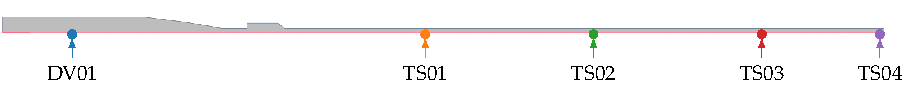
\includegraphics[width=5.75in]{../figures/STAR_new_geometry_colorlabels_tikz.pdf}};
    % \node[inner sep=0pt] (plot) at (0,-6){%% Creator: Matplotlib, PGF backend
%%
%% To include the figure in your LaTeX document, write
%%   \input{<filename>.pgf}
%%
%% Make sure the required packages are loaded in your preamble
%%   \usepackage{pgf}
%%
%% Also ensure that all the required font packages are loaded; for instance,
%% the lmodern package is sometimes necessary when using math font.
%%   \usepackage{lmodern}
%%
%% Figures using additional raster images can only be included by \input if
%% they are in the same directory as the main LaTeX file. For loading figures
%% from other directories you can use the `import` package
%%   \usepackage{import}
%%
%% and then include the figures with
%%   \import{<path to file>}{<filename>.pgf}
%%
%% Matplotlib used the following preamble
%%   \def\mathdefault#1{#1}
%%   \everymath=\expandafter{\the\everymath\displaystyle}
%%   \usepackage[utf8]{inputenc}
%%   \usepackage[T1]{fontenc}
%%   \usepackage[detect-all]{siunitx}
%%   \providecommand{\mathdefault}[1]{}
%%   \makeatletter\@ifpackageloaded{underscore}{}{\usepackage[strings]{underscore}}\makeatother
%%
\begingroup%
\makeatletter%
\begin{pgfpicture}%
\pgfpathrectangle{\pgfpointorigin}{\pgfqpoint{5.750000in}{4.312500in}}%
\pgfusepath{use as bounding box, clip}%
\begin{pgfscope}%
\pgfsetbuttcap%
\pgfsetmiterjoin%
\pgfsetlinewidth{0.000000pt}%
\definecolor{currentstroke}{rgb}{0.000000,0.000000,0.000000}%
\pgfsetstrokecolor{currentstroke}%
\pgfsetstrokeopacity{0.000000}%
\pgfsetdash{}{0pt}%
\pgfpathmoveto{\pgfqpoint{0.000000in}{0.000000in}}%
\pgfpathlineto{\pgfqpoint{5.750000in}{0.000000in}}%
\pgfpathlineto{\pgfqpoint{5.750000in}{4.312500in}}%
\pgfpathlineto{\pgfqpoint{0.000000in}{4.312500in}}%
\pgfpathlineto{\pgfqpoint{0.000000in}{0.000000in}}%
\pgfpathclose%
\pgfusepath{}%
\end{pgfscope}%
\begin{pgfscope}%
\pgfsetbuttcap%
\pgfsetmiterjoin%
\pgfsetlinewidth{0.000000pt}%
\definecolor{currentstroke}{rgb}{0.000000,0.000000,0.000000}%
\pgfsetstrokecolor{currentstroke}%
\pgfsetstrokeopacity{0.000000}%
\pgfsetdash{}{0pt}%
\pgfpathmoveto{\pgfqpoint{0.726769in}{0.580216in}}%
\pgfpathlineto{\pgfqpoint{5.585000in}{0.580216in}}%
\pgfpathlineto{\pgfqpoint{5.585000in}{4.147500in}}%
\pgfpathlineto{\pgfqpoint{0.726769in}{4.147500in}}%
\pgfpathlineto{\pgfqpoint{0.726769in}{0.580216in}}%
\pgfpathclose%
\pgfusepath{}%
\end{pgfscope}%
\begin{pgfscope}%
\pgfpathrectangle{\pgfqpoint{0.726769in}{0.580216in}}{\pgfqpoint{4.858231in}{3.567284in}}%
\pgfusepath{clip}%
\pgfsetrectcap%
\pgfsetroundjoin%
\pgfsetlinewidth{0.803000pt}%
\definecolor{currentstroke}{rgb}{0.690196,0.690196,0.690196}%
\pgfsetstrokecolor{currentstroke}%
\pgfsetdash{}{0pt}%
\pgfpathmoveto{\pgfqpoint{0.947576in}{0.580216in}}%
\pgfpathlineto{\pgfqpoint{0.947576in}{4.147500in}}%
\pgfusepath{stroke}%
\end{pgfscope}%
\begin{pgfscope}%
\pgfsetbuttcap%
\pgfsetroundjoin%
\definecolor{currentfill}{rgb}{0.000000,0.000000,0.000000}%
\pgfsetfillcolor{currentfill}%
\pgfsetlinewidth{0.803000pt}%
\definecolor{currentstroke}{rgb}{0.000000,0.000000,0.000000}%
\pgfsetstrokecolor{currentstroke}%
\pgfsetdash{}{0pt}%
\pgfsys@defobject{currentmarker}{\pgfqpoint{0.000000in}{-0.048611in}}{\pgfqpoint{0.000000in}{0.000000in}}{%
\pgfpathmoveto{\pgfqpoint{0.000000in}{0.000000in}}%
\pgfpathlineto{\pgfqpoint{0.000000in}{-0.048611in}}%
\pgfusepath{stroke,fill}%
}%
\begin{pgfscope}%
\pgfsys@transformshift{0.947576in}{0.580216in}%
\pgfsys@useobject{currentmarker}{}%
\end{pgfscope}%
\end{pgfscope}%
\begin{pgfscope}%
\definecolor{textcolor}{rgb}{0.000000,0.000000,0.000000}%
\pgfsetstrokecolor{textcolor}%
\pgfsetfillcolor{textcolor}%
\pgftext[x=0.947576in,y=0.482994in,,top]{\color{textcolor}{\rmfamily\fontsize{9.000000}{10.800000}\selectfont\catcode`\^=\active\def^{\ifmmode\sp\else\^{}\fi}\catcode`\%=\active\def%{\%}$\mathdefault{0.000}$}}%
\end{pgfscope}%
\begin{pgfscope}%
\pgfpathrectangle{\pgfqpoint{0.726769in}{0.580216in}}{\pgfqpoint{4.858231in}{3.567284in}}%
\pgfusepath{clip}%
\pgfsetrectcap%
\pgfsetroundjoin%
\pgfsetlinewidth{0.803000pt}%
\definecolor{currentstroke}{rgb}{0.690196,0.690196,0.690196}%
\pgfsetstrokecolor{currentstroke}%
\pgfsetdash{}{0pt}%
\pgfpathmoveto{\pgfqpoint{1.830899in}{0.580216in}}%
\pgfpathlineto{\pgfqpoint{1.830899in}{4.147500in}}%
\pgfusepath{stroke}%
\end{pgfscope}%
\begin{pgfscope}%
\pgfsetbuttcap%
\pgfsetroundjoin%
\definecolor{currentfill}{rgb}{0.000000,0.000000,0.000000}%
\pgfsetfillcolor{currentfill}%
\pgfsetlinewidth{0.803000pt}%
\definecolor{currentstroke}{rgb}{0.000000,0.000000,0.000000}%
\pgfsetstrokecolor{currentstroke}%
\pgfsetdash{}{0pt}%
\pgfsys@defobject{currentmarker}{\pgfqpoint{0.000000in}{-0.048611in}}{\pgfqpoint{0.000000in}{0.000000in}}{%
\pgfpathmoveto{\pgfqpoint{0.000000in}{0.000000in}}%
\pgfpathlineto{\pgfqpoint{0.000000in}{-0.048611in}}%
\pgfusepath{stroke,fill}%
}%
\begin{pgfscope}%
\pgfsys@transformshift{1.830899in}{0.580216in}%
\pgfsys@useobject{currentmarker}{}%
\end{pgfscope}%
\end{pgfscope}%
\begin{pgfscope}%
\definecolor{textcolor}{rgb}{0.000000,0.000000,0.000000}%
\pgfsetstrokecolor{textcolor}%
\pgfsetfillcolor{textcolor}%
\pgftext[x=1.830899in,y=0.482994in,,top]{\color{textcolor}{\rmfamily\fontsize{9.000000}{10.800000}\selectfont\catcode`\^=\active\def^{\ifmmode\sp\else\^{}\fi}\catcode`\%=\active\def%{\%}$\mathdefault{0.002}$}}%
\end{pgfscope}%
\begin{pgfscope}%
\pgfpathrectangle{\pgfqpoint{0.726769in}{0.580216in}}{\pgfqpoint{4.858231in}{3.567284in}}%
\pgfusepath{clip}%
\pgfsetrectcap%
\pgfsetroundjoin%
\pgfsetlinewidth{0.803000pt}%
\definecolor{currentstroke}{rgb}{0.690196,0.690196,0.690196}%
\pgfsetstrokecolor{currentstroke}%
\pgfsetdash{}{0pt}%
\pgfpathmoveto{\pgfqpoint{2.714223in}{0.580216in}}%
\pgfpathlineto{\pgfqpoint{2.714223in}{4.147500in}}%
\pgfusepath{stroke}%
\end{pgfscope}%
\begin{pgfscope}%
\pgfsetbuttcap%
\pgfsetroundjoin%
\definecolor{currentfill}{rgb}{0.000000,0.000000,0.000000}%
\pgfsetfillcolor{currentfill}%
\pgfsetlinewidth{0.803000pt}%
\definecolor{currentstroke}{rgb}{0.000000,0.000000,0.000000}%
\pgfsetstrokecolor{currentstroke}%
\pgfsetdash{}{0pt}%
\pgfsys@defobject{currentmarker}{\pgfqpoint{0.000000in}{-0.048611in}}{\pgfqpoint{0.000000in}{0.000000in}}{%
\pgfpathmoveto{\pgfqpoint{0.000000in}{0.000000in}}%
\pgfpathlineto{\pgfqpoint{0.000000in}{-0.048611in}}%
\pgfusepath{stroke,fill}%
}%
\begin{pgfscope}%
\pgfsys@transformshift{2.714223in}{0.580216in}%
\pgfsys@useobject{currentmarker}{}%
\end{pgfscope}%
\end{pgfscope}%
\begin{pgfscope}%
\definecolor{textcolor}{rgb}{0.000000,0.000000,0.000000}%
\pgfsetstrokecolor{textcolor}%
\pgfsetfillcolor{textcolor}%
\pgftext[x=2.714223in,y=0.482994in,,top]{\color{textcolor}{\rmfamily\fontsize{9.000000}{10.800000}\selectfont\catcode`\^=\active\def^{\ifmmode\sp\else\^{}\fi}\catcode`\%=\active\def%{\%}$\mathdefault{0.004}$}}%
\end{pgfscope}%
\begin{pgfscope}%
\pgfpathrectangle{\pgfqpoint{0.726769in}{0.580216in}}{\pgfqpoint{4.858231in}{3.567284in}}%
\pgfusepath{clip}%
\pgfsetrectcap%
\pgfsetroundjoin%
\pgfsetlinewidth{0.803000pt}%
\definecolor{currentstroke}{rgb}{0.690196,0.690196,0.690196}%
\pgfsetstrokecolor{currentstroke}%
\pgfsetdash{}{0pt}%
\pgfpathmoveto{\pgfqpoint{3.597546in}{0.580216in}}%
\pgfpathlineto{\pgfqpoint{3.597546in}{4.147500in}}%
\pgfusepath{stroke}%
\end{pgfscope}%
\begin{pgfscope}%
\pgfsetbuttcap%
\pgfsetroundjoin%
\definecolor{currentfill}{rgb}{0.000000,0.000000,0.000000}%
\pgfsetfillcolor{currentfill}%
\pgfsetlinewidth{0.803000pt}%
\definecolor{currentstroke}{rgb}{0.000000,0.000000,0.000000}%
\pgfsetstrokecolor{currentstroke}%
\pgfsetdash{}{0pt}%
\pgfsys@defobject{currentmarker}{\pgfqpoint{0.000000in}{-0.048611in}}{\pgfqpoint{0.000000in}{0.000000in}}{%
\pgfpathmoveto{\pgfqpoint{0.000000in}{0.000000in}}%
\pgfpathlineto{\pgfqpoint{0.000000in}{-0.048611in}}%
\pgfusepath{stroke,fill}%
}%
\begin{pgfscope}%
\pgfsys@transformshift{3.597546in}{0.580216in}%
\pgfsys@useobject{currentmarker}{}%
\end{pgfscope}%
\end{pgfscope}%
\begin{pgfscope}%
\definecolor{textcolor}{rgb}{0.000000,0.000000,0.000000}%
\pgfsetstrokecolor{textcolor}%
\pgfsetfillcolor{textcolor}%
\pgftext[x=3.597546in,y=0.482994in,,top]{\color{textcolor}{\rmfamily\fontsize{9.000000}{10.800000}\selectfont\catcode`\^=\active\def^{\ifmmode\sp\else\^{}\fi}\catcode`\%=\active\def%{\%}$\mathdefault{0.006}$}}%
\end{pgfscope}%
\begin{pgfscope}%
\pgfpathrectangle{\pgfqpoint{0.726769in}{0.580216in}}{\pgfqpoint{4.858231in}{3.567284in}}%
\pgfusepath{clip}%
\pgfsetrectcap%
\pgfsetroundjoin%
\pgfsetlinewidth{0.803000pt}%
\definecolor{currentstroke}{rgb}{0.690196,0.690196,0.690196}%
\pgfsetstrokecolor{currentstroke}%
\pgfsetdash{}{0pt}%
\pgfpathmoveto{\pgfqpoint{4.480870in}{0.580216in}}%
\pgfpathlineto{\pgfqpoint{4.480870in}{4.147500in}}%
\pgfusepath{stroke}%
\end{pgfscope}%
\begin{pgfscope}%
\pgfsetbuttcap%
\pgfsetroundjoin%
\definecolor{currentfill}{rgb}{0.000000,0.000000,0.000000}%
\pgfsetfillcolor{currentfill}%
\pgfsetlinewidth{0.803000pt}%
\definecolor{currentstroke}{rgb}{0.000000,0.000000,0.000000}%
\pgfsetstrokecolor{currentstroke}%
\pgfsetdash{}{0pt}%
\pgfsys@defobject{currentmarker}{\pgfqpoint{0.000000in}{-0.048611in}}{\pgfqpoint{0.000000in}{0.000000in}}{%
\pgfpathmoveto{\pgfqpoint{0.000000in}{0.000000in}}%
\pgfpathlineto{\pgfqpoint{0.000000in}{-0.048611in}}%
\pgfusepath{stroke,fill}%
}%
\begin{pgfscope}%
\pgfsys@transformshift{4.480870in}{0.580216in}%
\pgfsys@useobject{currentmarker}{}%
\end{pgfscope}%
\end{pgfscope}%
\begin{pgfscope}%
\definecolor{textcolor}{rgb}{0.000000,0.000000,0.000000}%
\pgfsetstrokecolor{textcolor}%
\pgfsetfillcolor{textcolor}%
\pgftext[x=4.480870in,y=0.482994in,,top]{\color{textcolor}{\rmfamily\fontsize{9.000000}{10.800000}\selectfont\catcode`\^=\active\def^{\ifmmode\sp\else\^{}\fi}\catcode`\%=\active\def%{\%}$\mathdefault{0.008}$}}%
\end{pgfscope}%
\begin{pgfscope}%
\pgfpathrectangle{\pgfqpoint{0.726769in}{0.580216in}}{\pgfqpoint{4.858231in}{3.567284in}}%
\pgfusepath{clip}%
\pgfsetrectcap%
\pgfsetroundjoin%
\pgfsetlinewidth{0.803000pt}%
\definecolor{currentstroke}{rgb}{0.690196,0.690196,0.690196}%
\pgfsetstrokecolor{currentstroke}%
\pgfsetdash{}{0pt}%
\pgfpathmoveto{\pgfqpoint{5.364193in}{0.580216in}}%
\pgfpathlineto{\pgfqpoint{5.364193in}{4.147500in}}%
\pgfusepath{stroke}%
\end{pgfscope}%
\begin{pgfscope}%
\pgfsetbuttcap%
\pgfsetroundjoin%
\definecolor{currentfill}{rgb}{0.000000,0.000000,0.000000}%
\pgfsetfillcolor{currentfill}%
\pgfsetlinewidth{0.803000pt}%
\definecolor{currentstroke}{rgb}{0.000000,0.000000,0.000000}%
\pgfsetstrokecolor{currentstroke}%
\pgfsetdash{}{0pt}%
\pgfsys@defobject{currentmarker}{\pgfqpoint{0.000000in}{-0.048611in}}{\pgfqpoint{0.000000in}{0.000000in}}{%
\pgfpathmoveto{\pgfqpoint{0.000000in}{0.000000in}}%
\pgfpathlineto{\pgfqpoint{0.000000in}{-0.048611in}}%
\pgfusepath{stroke,fill}%
}%
\begin{pgfscope}%
\pgfsys@transformshift{5.364193in}{0.580216in}%
\pgfsys@useobject{currentmarker}{}%
\end{pgfscope}%
\end{pgfscope}%
\begin{pgfscope}%
\definecolor{textcolor}{rgb}{0.000000,0.000000,0.000000}%
\pgfsetstrokecolor{textcolor}%
\pgfsetfillcolor{textcolor}%
\pgftext[x=5.364193in,y=0.482994in,,top]{\color{textcolor}{\rmfamily\fontsize{9.000000}{10.800000}\selectfont\catcode`\^=\active\def^{\ifmmode\sp\else\^{}\fi}\catcode`\%=\active\def%{\%}$\mathdefault{0.010}$}}%
\end{pgfscope}%
\begin{pgfscope}%
\definecolor{textcolor}{rgb}{0.000000,0.000000,0.000000}%
\pgfsetstrokecolor{textcolor}%
\pgfsetfillcolor{textcolor}%
\pgftext[x=3.155885in,y=0.317048in,,top]{\color{textcolor}{\rmfamily\fontsize{11.000000}{13.200000}\selectfont\catcode`\^=\active\def^{\ifmmode\sp\else\^{}\fi}\catcode`\%=\active\def%{\%}Time (\si{\second})}}%
\end{pgfscope}%
\begin{pgfscope}%
\pgfpathrectangle{\pgfqpoint{0.726769in}{0.580216in}}{\pgfqpoint{4.858231in}{3.567284in}}%
\pgfusepath{clip}%
\pgfsetrectcap%
\pgfsetroundjoin%
\pgfsetlinewidth{0.803000pt}%
\definecolor{currentstroke}{rgb}{0.690196,0.690196,0.690196}%
\pgfsetstrokecolor{currentstroke}%
\pgfsetdash{}{0pt}%
\pgfpathmoveto{\pgfqpoint{0.726769in}{0.649188in}}%
\pgfpathlineto{\pgfqpoint{5.585000in}{0.649188in}}%
\pgfusepath{stroke}%
\end{pgfscope}%
\begin{pgfscope}%
\pgfsetbuttcap%
\pgfsetroundjoin%
\definecolor{currentfill}{rgb}{0.000000,0.000000,0.000000}%
\pgfsetfillcolor{currentfill}%
\pgfsetlinewidth{0.803000pt}%
\definecolor{currentstroke}{rgb}{0.000000,0.000000,0.000000}%
\pgfsetstrokecolor{currentstroke}%
\pgfsetdash{}{0pt}%
\pgfsys@defobject{currentmarker}{\pgfqpoint{-0.048611in}{0.000000in}}{\pgfqpoint{-0.000000in}{0.000000in}}{%
\pgfpathmoveto{\pgfqpoint{-0.000000in}{0.000000in}}%
\pgfpathlineto{\pgfqpoint{-0.048611in}{0.000000in}}%
\pgfusepath{stroke,fill}%
}%
\begin{pgfscope}%
\pgfsys@transformshift{0.726769in}{0.649188in}%
\pgfsys@useobject{currentmarker}{}%
\end{pgfscope}%
\end{pgfscope}%
\begin{pgfscope}%
\definecolor{textcolor}{rgb}{0.000000,0.000000,0.000000}%
\pgfsetstrokecolor{textcolor}%
\pgfsetfillcolor{textcolor}%
\pgftext[x=0.565311in, y=0.606143in, left, base]{\color{textcolor}{\rmfamily\fontsize{9.000000}{10.800000}\selectfont\catcode`\^=\active\def^{\ifmmode\sp\else\^{}\fi}\catcode`\%=\active\def%{\%}$\mathdefault{0}$}}%
\end{pgfscope}%
\begin{pgfscope}%
\pgfpathrectangle{\pgfqpoint{0.726769in}{0.580216in}}{\pgfqpoint{4.858231in}{3.567284in}}%
\pgfusepath{clip}%
\pgfsetrectcap%
\pgfsetroundjoin%
\pgfsetlinewidth{0.803000pt}%
\definecolor{currentstroke}{rgb}{0.690196,0.690196,0.690196}%
\pgfsetstrokecolor{currentstroke}%
\pgfsetdash{}{0pt}%
\pgfpathmoveto{\pgfqpoint{0.726769in}{1.215067in}}%
\pgfpathlineto{\pgfqpoint{5.585000in}{1.215067in}}%
\pgfusepath{stroke}%
\end{pgfscope}%
\begin{pgfscope}%
\pgfsetbuttcap%
\pgfsetroundjoin%
\definecolor{currentfill}{rgb}{0.000000,0.000000,0.000000}%
\pgfsetfillcolor{currentfill}%
\pgfsetlinewidth{0.803000pt}%
\definecolor{currentstroke}{rgb}{0.000000,0.000000,0.000000}%
\pgfsetstrokecolor{currentstroke}%
\pgfsetdash{}{0pt}%
\pgfsys@defobject{currentmarker}{\pgfqpoint{-0.048611in}{0.000000in}}{\pgfqpoint{-0.000000in}{0.000000in}}{%
\pgfpathmoveto{\pgfqpoint{-0.000000in}{0.000000in}}%
\pgfpathlineto{\pgfqpoint{-0.048611in}{0.000000in}}%
\pgfusepath{stroke,fill}%
}%
\begin{pgfscope}%
\pgfsys@transformshift{0.726769in}{1.215067in}%
\pgfsys@useobject{currentmarker}{}%
\end{pgfscope}%
\end{pgfscope}%
\begin{pgfscope}%
\definecolor{textcolor}{rgb}{0.000000,0.000000,0.000000}%
\pgfsetstrokecolor{textcolor}%
\pgfsetfillcolor{textcolor}%
\pgftext[x=0.436840in, y=1.172022in, left, base]{\color{textcolor}{\rmfamily\fontsize{9.000000}{10.800000}\selectfont\catcode`\^=\active\def^{\ifmmode\sp\else\^{}\fi}\catcode`\%=\active\def%{\%}$\mathdefault{500}$}}%
\end{pgfscope}%
\begin{pgfscope}%
\pgfpathrectangle{\pgfqpoint{0.726769in}{0.580216in}}{\pgfqpoint{4.858231in}{3.567284in}}%
\pgfusepath{clip}%
\pgfsetrectcap%
\pgfsetroundjoin%
\pgfsetlinewidth{0.803000pt}%
\definecolor{currentstroke}{rgb}{0.690196,0.690196,0.690196}%
\pgfsetstrokecolor{currentstroke}%
\pgfsetdash{}{0pt}%
\pgfpathmoveto{\pgfqpoint{0.726769in}{1.780945in}}%
\pgfpathlineto{\pgfqpoint{5.585000in}{1.780945in}}%
\pgfusepath{stroke}%
\end{pgfscope}%
\begin{pgfscope}%
\pgfsetbuttcap%
\pgfsetroundjoin%
\definecolor{currentfill}{rgb}{0.000000,0.000000,0.000000}%
\pgfsetfillcolor{currentfill}%
\pgfsetlinewidth{0.803000pt}%
\definecolor{currentstroke}{rgb}{0.000000,0.000000,0.000000}%
\pgfsetstrokecolor{currentstroke}%
\pgfsetdash{}{0pt}%
\pgfsys@defobject{currentmarker}{\pgfqpoint{-0.048611in}{0.000000in}}{\pgfqpoint{-0.000000in}{0.000000in}}{%
\pgfpathmoveto{\pgfqpoint{-0.000000in}{0.000000in}}%
\pgfpathlineto{\pgfqpoint{-0.048611in}{0.000000in}}%
\pgfusepath{stroke,fill}%
}%
\begin{pgfscope}%
\pgfsys@transformshift{0.726769in}{1.780945in}%
\pgfsys@useobject{currentmarker}{}%
\end{pgfscope}%
\end{pgfscope}%
\begin{pgfscope}%
\definecolor{textcolor}{rgb}{0.000000,0.000000,0.000000}%
\pgfsetstrokecolor{textcolor}%
\pgfsetfillcolor{textcolor}%
\pgftext[x=0.372604in, y=1.737900in, left, base]{\color{textcolor}{\rmfamily\fontsize{9.000000}{10.800000}\selectfont\catcode`\^=\active\def^{\ifmmode\sp\else\^{}\fi}\catcode`\%=\active\def%{\%}$\mathdefault{1000}$}}%
\end{pgfscope}%
\begin{pgfscope}%
\pgfpathrectangle{\pgfqpoint{0.726769in}{0.580216in}}{\pgfqpoint{4.858231in}{3.567284in}}%
\pgfusepath{clip}%
\pgfsetrectcap%
\pgfsetroundjoin%
\pgfsetlinewidth{0.803000pt}%
\definecolor{currentstroke}{rgb}{0.690196,0.690196,0.690196}%
\pgfsetstrokecolor{currentstroke}%
\pgfsetdash{}{0pt}%
\pgfpathmoveto{\pgfqpoint{0.726769in}{2.346824in}}%
\pgfpathlineto{\pgfqpoint{5.585000in}{2.346824in}}%
\pgfusepath{stroke}%
\end{pgfscope}%
\begin{pgfscope}%
\pgfsetbuttcap%
\pgfsetroundjoin%
\definecolor{currentfill}{rgb}{0.000000,0.000000,0.000000}%
\pgfsetfillcolor{currentfill}%
\pgfsetlinewidth{0.803000pt}%
\definecolor{currentstroke}{rgb}{0.000000,0.000000,0.000000}%
\pgfsetstrokecolor{currentstroke}%
\pgfsetdash{}{0pt}%
\pgfsys@defobject{currentmarker}{\pgfqpoint{-0.048611in}{0.000000in}}{\pgfqpoint{-0.000000in}{0.000000in}}{%
\pgfpathmoveto{\pgfqpoint{-0.000000in}{0.000000in}}%
\pgfpathlineto{\pgfqpoint{-0.048611in}{0.000000in}}%
\pgfusepath{stroke,fill}%
}%
\begin{pgfscope}%
\pgfsys@transformshift{0.726769in}{2.346824in}%
\pgfsys@useobject{currentmarker}{}%
\end{pgfscope}%
\end{pgfscope}%
\begin{pgfscope}%
\definecolor{textcolor}{rgb}{0.000000,0.000000,0.000000}%
\pgfsetstrokecolor{textcolor}%
\pgfsetfillcolor{textcolor}%
\pgftext[x=0.372604in, y=2.303779in, left, base]{\color{textcolor}{\rmfamily\fontsize{9.000000}{10.800000}\selectfont\catcode`\^=\active\def^{\ifmmode\sp\else\^{}\fi}\catcode`\%=\active\def%{\%}$\mathdefault{1500}$}}%
\end{pgfscope}%
\begin{pgfscope}%
\pgfpathrectangle{\pgfqpoint{0.726769in}{0.580216in}}{\pgfqpoint{4.858231in}{3.567284in}}%
\pgfusepath{clip}%
\pgfsetrectcap%
\pgfsetroundjoin%
\pgfsetlinewidth{0.803000pt}%
\definecolor{currentstroke}{rgb}{0.690196,0.690196,0.690196}%
\pgfsetstrokecolor{currentstroke}%
\pgfsetdash{}{0pt}%
\pgfpathmoveto{\pgfqpoint{0.726769in}{2.912702in}}%
\pgfpathlineto{\pgfqpoint{5.585000in}{2.912702in}}%
\pgfusepath{stroke}%
\end{pgfscope}%
\begin{pgfscope}%
\pgfsetbuttcap%
\pgfsetroundjoin%
\definecolor{currentfill}{rgb}{0.000000,0.000000,0.000000}%
\pgfsetfillcolor{currentfill}%
\pgfsetlinewidth{0.803000pt}%
\definecolor{currentstroke}{rgb}{0.000000,0.000000,0.000000}%
\pgfsetstrokecolor{currentstroke}%
\pgfsetdash{}{0pt}%
\pgfsys@defobject{currentmarker}{\pgfqpoint{-0.048611in}{0.000000in}}{\pgfqpoint{-0.000000in}{0.000000in}}{%
\pgfpathmoveto{\pgfqpoint{-0.000000in}{0.000000in}}%
\pgfpathlineto{\pgfqpoint{-0.048611in}{0.000000in}}%
\pgfusepath{stroke,fill}%
}%
\begin{pgfscope}%
\pgfsys@transformshift{0.726769in}{2.912702in}%
\pgfsys@useobject{currentmarker}{}%
\end{pgfscope}%
\end{pgfscope}%
\begin{pgfscope}%
\definecolor{textcolor}{rgb}{0.000000,0.000000,0.000000}%
\pgfsetstrokecolor{textcolor}%
\pgfsetfillcolor{textcolor}%
\pgftext[x=0.372604in, y=2.869657in, left, base]{\color{textcolor}{\rmfamily\fontsize{9.000000}{10.800000}\selectfont\catcode`\^=\active\def^{\ifmmode\sp\else\^{}\fi}\catcode`\%=\active\def%{\%}$\mathdefault{2000}$}}%
\end{pgfscope}%
\begin{pgfscope}%
\pgfpathrectangle{\pgfqpoint{0.726769in}{0.580216in}}{\pgfqpoint{4.858231in}{3.567284in}}%
\pgfusepath{clip}%
\pgfsetrectcap%
\pgfsetroundjoin%
\pgfsetlinewidth{0.803000pt}%
\definecolor{currentstroke}{rgb}{0.690196,0.690196,0.690196}%
\pgfsetstrokecolor{currentstroke}%
\pgfsetdash{}{0pt}%
\pgfpathmoveto{\pgfqpoint{0.726769in}{3.478581in}}%
\pgfpathlineto{\pgfqpoint{5.585000in}{3.478581in}}%
\pgfusepath{stroke}%
\end{pgfscope}%
\begin{pgfscope}%
\pgfsetbuttcap%
\pgfsetroundjoin%
\definecolor{currentfill}{rgb}{0.000000,0.000000,0.000000}%
\pgfsetfillcolor{currentfill}%
\pgfsetlinewidth{0.803000pt}%
\definecolor{currentstroke}{rgb}{0.000000,0.000000,0.000000}%
\pgfsetstrokecolor{currentstroke}%
\pgfsetdash{}{0pt}%
\pgfsys@defobject{currentmarker}{\pgfqpoint{-0.048611in}{0.000000in}}{\pgfqpoint{-0.000000in}{0.000000in}}{%
\pgfpathmoveto{\pgfqpoint{-0.000000in}{0.000000in}}%
\pgfpathlineto{\pgfqpoint{-0.048611in}{0.000000in}}%
\pgfusepath{stroke,fill}%
}%
\begin{pgfscope}%
\pgfsys@transformshift{0.726769in}{3.478581in}%
\pgfsys@useobject{currentmarker}{}%
\end{pgfscope}%
\end{pgfscope}%
\begin{pgfscope}%
\definecolor{textcolor}{rgb}{0.000000,0.000000,0.000000}%
\pgfsetstrokecolor{textcolor}%
\pgfsetfillcolor{textcolor}%
\pgftext[x=0.372604in, y=3.435536in, left, base]{\color{textcolor}{\rmfamily\fontsize{9.000000}{10.800000}\selectfont\catcode`\^=\active\def^{\ifmmode\sp\else\^{}\fi}\catcode`\%=\active\def%{\%}$\mathdefault{2500}$}}%
\end{pgfscope}%
\begin{pgfscope}%
\pgfpathrectangle{\pgfqpoint{0.726769in}{0.580216in}}{\pgfqpoint{4.858231in}{3.567284in}}%
\pgfusepath{clip}%
\pgfsetrectcap%
\pgfsetroundjoin%
\pgfsetlinewidth{0.803000pt}%
\definecolor{currentstroke}{rgb}{0.690196,0.690196,0.690196}%
\pgfsetstrokecolor{currentstroke}%
\pgfsetdash{}{0pt}%
\pgfpathmoveto{\pgfqpoint{0.726769in}{4.044459in}}%
\pgfpathlineto{\pgfqpoint{5.585000in}{4.044459in}}%
\pgfusepath{stroke}%
\end{pgfscope}%
\begin{pgfscope}%
\pgfsetbuttcap%
\pgfsetroundjoin%
\definecolor{currentfill}{rgb}{0.000000,0.000000,0.000000}%
\pgfsetfillcolor{currentfill}%
\pgfsetlinewidth{0.803000pt}%
\definecolor{currentstroke}{rgb}{0.000000,0.000000,0.000000}%
\pgfsetstrokecolor{currentstroke}%
\pgfsetdash{}{0pt}%
\pgfsys@defobject{currentmarker}{\pgfqpoint{-0.048611in}{0.000000in}}{\pgfqpoint{-0.000000in}{0.000000in}}{%
\pgfpathmoveto{\pgfqpoint{-0.000000in}{0.000000in}}%
\pgfpathlineto{\pgfqpoint{-0.048611in}{0.000000in}}%
\pgfusepath{stroke,fill}%
}%
\begin{pgfscope}%
\pgfsys@transformshift{0.726769in}{4.044459in}%
\pgfsys@useobject{currentmarker}{}%
\end{pgfscope}%
\end{pgfscope}%
\begin{pgfscope}%
\definecolor{textcolor}{rgb}{0.000000,0.000000,0.000000}%
\pgfsetstrokecolor{textcolor}%
\pgfsetfillcolor{textcolor}%
\pgftext[x=0.372604in, y=4.001414in, left, base]{\color{textcolor}{\rmfamily\fontsize{9.000000}{10.800000}\selectfont\catcode`\^=\active\def^{\ifmmode\sp\else\^{}\fi}\catcode`\%=\active\def%{\%}$\mathdefault{3000}$}}%
\end{pgfscope}%
\begin{pgfscope}%
\definecolor{textcolor}{rgb}{0.000000,0.000000,0.000000}%
\pgfsetstrokecolor{textcolor}%
\pgfsetfillcolor{textcolor}%
\pgftext[x=0.317048in,y=2.363858in,,bottom,rotate=90.000000]{\color{textcolor}{\rmfamily\fontsize{11.000000}{13.200000}\selectfont\catcode`\^=\active\def^{\ifmmode\sp\else\^{}\fi}\catcode`\%=\active\def%{\%}Temperature (\si{\kelvin})}}%
\end{pgfscope}%
\begin{pgfscope}%
\pgfpathrectangle{\pgfqpoint{0.726769in}{0.580216in}}{\pgfqpoint{4.858231in}{3.567284in}}%
\pgfusepath{clip}%
\pgfsetrectcap%
\pgfsetroundjoin%
\pgfsetlinewidth{1.505625pt}%
\definecolor{currentstroke}{rgb}{0.121569,0.466667,0.705882}%
\pgfsetstrokecolor{currentstroke}%
\pgfsetdash{}{0pt}%
\pgfpathmoveto{\pgfqpoint{0.947598in}{0.981472in}}%
\pgfpathlineto{\pgfqpoint{1.030255in}{0.981470in}}%
\pgfpathlineto{\pgfqpoint{1.032110in}{0.979405in}}%
\pgfpathlineto{\pgfqpoint{1.036747in}{0.975685in}}%
\pgfpathlineto{\pgfqpoint{1.041407in}{0.973083in}}%
\pgfpathlineto{\pgfqpoint{1.046972in}{0.971134in}}%
\pgfpathlineto{\pgfqpoint{1.055341in}{0.970413in}}%
\pgfpathlineto{\pgfqpoint{1.075768in}{0.972271in}}%
\pgfpathlineto{\pgfqpoint{1.076695in}{0.975586in}}%
\pgfpathlineto{\pgfqpoint{1.077623in}{0.975947in}}%
\pgfpathlineto{\pgfqpoint{1.079478in}{0.975172in}}%
\pgfpathlineto{\pgfqpoint{1.080405in}{0.974899in}}%
\pgfpathlineto{\pgfqpoint{1.082260in}{0.975086in}}%
\pgfpathlineto{\pgfqpoint{1.084115in}{0.974417in}}%
\pgfpathlineto{\pgfqpoint{1.087847in}{0.974030in}}%
\pgfpathlineto{\pgfqpoint{1.089702in}{0.974452in}}%
\pgfpathlineto{\pgfqpoint{1.094340in}{0.970791in}}%
\pgfpathlineto{\pgfqpoint{1.102709in}{0.965731in}}%
\pgfpathlineto{\pgfqpoint{1.110129in}{0.963119in}}%
\pgfpathlineto{\pgfqpoint{1.117571in}{0.961962in}}%
\pgfpathlineto{\pgfqpoint{1.120354in}{0.962114in}}%
\pgfpathlineto{\pgfqpoint{1.124064in}{0.962139in}}%
\pgfpathlineto{\pgfqpoint{1.127774in}{0.962674in}}%
\pgfpathlineto{\pgfqpoint{1.132433in}{0.963073in}}%
\pgfpathlineto{\pgfqpoint{1.137071in}{0.963765in}}%
\pgfpathlineto{\pgfqpoint{1.137998in}{0.963166in}}%
\pgfpathlineto{\pgfqpoint{1.138926in}{0.966518in}}%
\pgfpathlineto{\pgfqpoint{1.139853in}{0.966985in}}%
\pgfpathlineto{\pgfqpoint{1.141708in}{0.966558in}}%
\pgfpathlineto{\pgfqpoint{1.143563in}{0.966427in}}%
\pgfpathlineto{\pgfqpoint{1.146368in}{0.966261in}}%
\pgfpathlineto{\pgfqpoint{1.148223in}{0.966088in}}%
\pgfpathlineto{\pgfqpoint{1.152860in}{0.965633in}}%
\pgfpathlineto{\pgfqpoint{1.162157in}{0.964647in}}%
\pgfpathlineto{\pgfqpoint{1.164012in}{0.964696in}}%
\pgfpathlineto{\pgfqpoint{1.166794in}{0.964359in}}%
\pgfpathlineto{\pgfqpoint{1.175142in}{0.962944in}}%
\pgfpathlineto{\pgfqpoint{1.178874in}{0.962636in}}%
\pgfpathlineto{\pgfqpoint{1.187221in}{0.961285in}}%
\pgfpathlineto{\pgfqpoint{1.190931in}{0.961088in}}%
\pgfpathlineto{\pgfqpoint{1.193736in}{0.960527in}}%
\pgfpathlineto{\pgfqpoint{1.202083in}{0.959427in}}%
\pgfpathlineto{\pgfqpoint{1.206743in}{0.959079in}}%
\pgfpathlineto{\pgfqpoint{1.209525in}{0.958810in}}%
\pgfpathlineto{\pgfqpoint{1.217873in}{0.957217in}}%
\pgfpathlineto{\pgfqpoint{1.221605in}{0.956896in}}%
\pgfpathlineto{\pgfqpoint{1.224387in}{0.956170in}}%
\pgfpathlineto{\pgfqpoint{1.238322in}{0.953306in}}%
\pgfpathlineto{\pgfqpoint{1.242032in}{0.953153in}}%
\pgfpathlineto{\pgfqpoint{1.246669in}{0.953338in}}%
\pgfpathlineto{\pgfqpoint{1.252256in}{0.953434in}}%
\pgfpathlineto{\pgfqpoint{1.258748in}{0.954057in}}%
\pgfpathlineto{\pgfqpoint{1.265241in}{0.953495in}}%
\pgfpathlineto{\pgfqpoint{1.270828in}{0.953829in}}%
\pgfpathlineto{\pgfqpoint{1.276393in}{0.953339in}}%
\pgfpathlineto{\pgfqpoint{1.282907in}{0.951091in}}%
\pgfpathlineto{\pgfqpoint{1.286617in}{0.950589in}}%
\pgfpathlineto{\pgfqpoint{1.288472in}{0.950072in}}%
\pgfpathlineto{\pgfqpoint{1.290327in}{0.948717in}}%
\pgfpathlineto{\pgfqpoint{1.293110in}{0.948687in}}%
\pgfpathlineto{\pgfqpoint{1.304262in}{0.947449in}}%
\pgfpathlineto{\pgfqpoint{1.307972in}{0.947268in}}%
\pgfpathlineto{\pgfqpoint{1.311682in}{0.947753in}}%
\pgfpathlineto{\pgfqpoint{1.317269in}{0.948284in}}%
\pgfpathlineto{\pgfqpoint{1.322834in}{0.949807in}}%
\pgfpathlineto{\pgfqpoint{1.325616in}{0.949700in}}%
\pgfpathlineto{\pgfqpoint{1.328421in}{0.950281in}}%
\pgfpathlineto{\pgfqpoint{1.334913in}{0.951640in}}%
\pgfpathlineto{\pgfqpoint{1.336768in}{0.952062in}}%
\pgfpathlineto{\pgfqpoint{1.359072in}{0.946344in}}%
\pgfpathlineto{\pgfqpoint{1.361854in}{0.945735in}}%
\pgfpathlineto{\pgfqpoint{1.363709in}{0.945136in}}%
\pgfpathlineto{\pgfqpoint{1.365564in}{0.944972in}}%
\pgfpathlineto{\pgfqpoint{1.367419in}{0.944420in}}%
\pgfpathlineto{\pgfqpoint{1.372057in}{0.944445in}}%
\pgfpathlineto{\pgfqpoint{1.374861in}{0.943634in}}%
\pgfpathlineto{\pgfqpoint{1.376716in}{0.943531in}}%
\pgfpathlineto{\pgfqpoint{1.379499in}{0.942930in}}%
\pgfpathlineto{\pgfqpoint{1.382281in}{0.942307in}}%
\pgfpathlineto{\pgfqpoint{1.383209in}{0.942048in}}%
\pgfpathlineto{\pgfqpoint{1.385991in}{0.942316in}}%
\pgfpathlineto{\pgfqpoint{1.392506in}{0.942212in}}%
\pgfpathlineto{\pgfqpoint{1.406440in}{0.941749in}}%
\pgfpathlineto{\pgfqpoint{1.412005in}{0.940364in}}%
\pgfpathlineto{\pgfqpoint{1.420375in}{0.939919in}}%
\pgfpathlineto{\pgfqpoint{1.423157in}{0.939699in}}%
\pgfpathlineto{\pgfqpoint{1.430577in}{0.938654in}}%
\pgfpathlineto{\pgfqpoint{1.434287in}{0.938657in}}%
\pgfpathlineto{\pgfqpoint{1.438019in}{0.938631in}}%
\pgfpathlineto{\pgfqpoint{1.442656in}{0.938604in}}%
\pgfpathlineto{\pgfqpoint{1.446366in}{0.938743in}}%
\pgfpathlineto{\pgfqpoint{1.455663in}{0.938293in}}%
\pgfpathlineto{\pgfqpoint{1.467743in}{0.937312in}}%
\pgfpathlineto{\pgfqpoint{1.471453in}{0.937232in}}%
\pgfpathlineto{\pgfqpoint{1.475163in}{0.936375in}}%
\pgfpathlineto{\pgfqpoint{1.482605in}{0.935587in}}%
\pgfpathlineto{\pgfqpoint{1.490025in}{0.935310in}}%
\pgfpathlineto{\pgfqpoint{1.494662in}{0.934885in}}%
\pgfpathlineto{\pgfqpoint{1.499322in}{0.934468in}}%
\pgfpathlineto{\pgfqpoint{1.507669in}{0.935136in}}%
\pgfpathlineto{\pgfqpoint{1.516966in}{0.935975in}}%
\pgfpathlineto{\pgfqpoint{1.528118in}{0.935129in}}%
\pgfpathlineto{\pgfqpoint{1.530900in}{0.934827in}}%
\pgfpathlineto{\pgfqpoint{1.534610in}{0.934596in}}%
\pgfpathlineto{\pgfqpoint{1.538320in}{0.933946in}}%
\pgfpathlineto{\pgfqpoint{1.543907in}{0.932183in}}%
\pgfpathlineto{\pgfqpoint{1.546690in}{0.931299in}}%
\pgfpathlineto{\pgfqpoint{1.548545in}{0.930843in}}%
\pgfpathlineto{\pgfqpoint{1.550400in}{0.930368in}}%
\pgfpathlineto{\pgfqpoint{1.553182in}{0.929469in}}%
\pgfpathlineto{\pgfqpoint{1.555037in}{0.929439in}}%
\pgfpathlineto{\pgfqpoint{1.560624in}{0.928642in}}%
\pgfpathlineto{\pgfqpoint{1.562479in}{0.928608in}}%
\pgfpathlineto{\pgfqpoint{1.568044in}{0.927923in}}%
\pgfpathlineto{\pgfqpoint{1.571776in}{0.927958in}}%
\pgfpathlineto{\pgfqpoint{1.589421in}{0.928098in}}%
\pgfpathlineto{\pgfqpoint{1.592203in}{0.928637in}}%
\pgfpathlineto{\pgfqpoint{1.593131in}{0.928388in}}%
\pgfpathlineto{\pgfqpoint{1.594058in}{0.935273in}}%
\pgfpathlineto{\pgfqpoint{1.594986in}{0.937231in}}%
\pgfpathlineto{\pgfqpoint{1.595913in}{0.937547in}}%
\pgfpathlineto{\pgfqpoint{1.596841in}{0.936900in}}%
\pgfpathlineto{\pgfqpoint{1.597768in}{0.935668in}}%
\pgfpathlineto{\pgfqpoint{1.598696in}{0.936237in}}%
\pgfpathlineto{\pgfqpoint{1.599623in}{0.937323in}}%
\pgfpathlineto{\pgfqpoint{1.600550in}{0.936530in}}%
\pgfpathlineto{\pgfqpoint{1.601478in}{0.936769in}}%
\pgfpathlineto{\pgfqpoint{1.602428in}{0.934671in}}%
\pgfpathlineto{\pgfqpoint{1.603355in}{0.933609in}}%
\pgfpathlineto{\pgfqpoint{1.604283in}{0.936077in}}%
\pgfpathlineto{\pgfqpoint{1.607065in}{0.935049in}}%
\pgfpathlineto{\pgfqpoint{1.608920in}{0.934658in}}%
\pgfpathlineto{\pgfqpoint{1.609847in}{0.935270in}}%
\pgfpathlineto{\pgfqpoint{1.610775in}{0.933563in}}%
\pgfpathlineto{\pgfqpoint{1.611702in}{0.934241in}}%
\pgfpathlineto{\pgfqpoint{1.613557in}{0.940006in}}%
\pgfpathlineto{\pgfqpoint{1.616340in}{0.937466in}}%
\pgfpathlineto{\pgfqpoint{1.617289in}{0.937507in}}%
\pgfpathlineto{\pgfqpoint{1.618217in}{0.938854in}}%
\pgfpathlineto{\pgfqpoint{1.620072in}{0.936747in}}%
\pgfpathlineto{\pgfqpoint{1.621927in}{0.936204in}}%
\pgfpathlineto{\pgfqpoint{1.623782in}{0.936548in}}%
\pgfpathlineto{\pgfqpoint{1.625637in}{0.936064in}}%
\pgfpathlineto{\pgfqpoint{1.628419in}{0.936252in}}%
\pgfpathlineto{\pgfqpoint{1.631202in}{0.935626in}}%
\pgfpathlineto{\pgfqpoint{1.633079in}{0.936700in}}%
\pgfpathlineto{\pgfqpoint{1.634006in}{0.937435in}}%
\pgfpathlineto{\pgfqpoint{1.635861in}{0.937515in}}%
\pgfpathlineto{\pgfqpoint{1.637716in}{0.938329in}}%
\pgfpathlineto{\pgfqpoint{1.640499in}{0.936693in}}%
\pgfpathlineto{\pgfqpoint{1.641426in}{0.936653in}}%
\pgfpathlineto{\pgfqpoint{1.643281in}{0.937696in}}%
\pgfpathlineto{\pgfqpoint{1.646991in}{0.936394in}}%
\pgfpathlineto{\pgfqpoint{1.647941in}{0.936824in}}%
\pgfpathlineto{\pgfqpoint{1.652578in}{0.935260in}}%
\pgfpathlineto{\pgfqpoint{1.653506in}{0.935952in}}%
\pgfpathlineto{\pgfqpoint{1.654433in}{0.936171in}}%
\pgfpathlineto{\pgfqpoint{1.658143in}{0.935637in}}%
\pgfpathlineto{\pgfqpoint{1.659071in}{0.936293in}}%
\pgfpathlineto{\pgfqpoint{1.660926in}{0.945303in}}%
\pgfpathlineto{\pgfqpoint{1.662803in}{0.943812in}}%
\pgfpathlineto{\pgfqpoint{1.663730in}{0.944736in}}%
\pgfpathlineto{\pgfqpoint{1.666513in}{0.944646in}}%
\pgfpathlineto{\pgfqpoint{1.667440in}{0.943243in}}%
\pgfpathlineto{\pgfqpoint{1.668368in}{0.943113in}}%
\pgfpathlineto{\pgfqpoint{1.669295in}{0.943791in}}%
\pgfpathlineto{\pgfqpoint{1.672078in}{0.943088in}}%
\pgfpathlineto{\pgfqpoint{1.673005in}{0.943782in}}%
\pgfpathlineto{\pgfqpoint{1.673933in}{0.943603in}}%
\pgfpathlineto{\pgfqpoint{1.675788in}{0.942251in}}%
\pgfpathlineto{\pgfqpoint{1.676715in}{0.948577in}}%
\pgfpathlineto{\pgfqpoint{1.677643in}{0.949206in}}%
\pgfpathlineto{\pgfqpoint{1.678592in}{0.948106in}}%
\pgfpathlineto{\pgfqpoint{1.683230in}{0.946767in}}%
\pgfpathlineto{\pgfqpoint{1.689722in}{0.946579in}}%
\pgfpathlineto{\pgfqpoint{1.695309in}{0.946511in}}%
\pgfpathlineto{\pgfqpoint{1.697164in}{0.947876in}}%
\pgfpathlineto{\pgfqpoint{1.698091in}{0.947395in}}%
\pgfpathlineto{\pgfqpoint{1.700874in}{0.948767in}}%
\pgfpathlineto{\pgfqpoint{1.701801in}{0.948363in}}%
\pgfpathlineto{\pgfqpoint{1.703656in}{0.946702in}}%
\pgfpathlineto{\pgfqpoint{1.706439in}{0.947478in}}%
\pgfpathlineto{\pgfqpoint{1.709243in}{0.946138in}}%
\pgfpathlineto{\pgfqpoint{1.711098in}{0.946712in}}%
\pgfpathlineto{\pgfqpoint{1.713881in}{0.945031in}}%
\pgfpathlineto{\pgfqpoint{1.715736in}{0.944478in}}%
\pgfpathlineto{\pgfqpoint{1.719446in}{0.944676in}}%
\pgfpathlineto{\pgfqpoint{1.722228in}{0.943547in}}%
\pgfpathlineto{\pgfqpoint{1.724105in}{0.944457in}}%
\pgfpathlineto{\pgfqpoint{1.727815in}{0.943484in}}%
\pgfpathlineto{\pgfqpoint{1.730598in}{0.943593in}}%
\pgfpathlineto{\pgfqpoint{1.732453in}{0.943200in}}%
\pgfpathlineto{\pgfqpoint{1.733380in}{0.942873in}}%
\pgfpathlineto{\pgfqpoint{1.735235in}{0.943162in}}%
\pgfpathlineto{\pgfqpoint{1.739895in}{0.941974in}}%
\pgfpathlineto{\pgfqpoint{1.741750in}{0.942747in}}%
\pgfpathlineto{\pgfqpoint{1.745460in}{0.942807in}}%
\pgfpathlineto{\pgfqpoint{1.748242in}{0.942680in}}%
\pgfpathlineto{\pgfqpoint{1.750097in}{0.943030in}}%
\pgfpathlineto{\pgfqpoint{1.752880in}{0.942869in}}%
\pgfpathlineto{\pgfqpoint{1.755684in}{0.943602in}}%
\pgfpathlineto{\pgfqpoint{1.759394in}{0.943546in}}%
\pgfpathlineto{\pgfqpoint{1.762177in}{0.943577in}}%
\pgfpathlineto{\pgfqpoint{1.764032in}{0.943699in}}%
\pgfpathlineto{\pgfqpoint{1.765887in}{0.944274in}}%
\pgfpathlineto{\pgfqpoint{1.767742in}{0.944326in}}%
\pgfpathlineto{\pgfqpoint{1.769619in}{0.945020in}}%
\pgfpathlineto{\pgfqpoint{1.771474in}{0.944996in}}%
\pgfpathlineto{\pgfqpoint{1.778894in}{0.946647in}}%
\pgfpathlineto{\pgfqpoint{1.782603in}{0.947302in}}%
\pgfpathlineto{\pgfqpoint{1.785408in}{0.947829in}}%
\pgfpathlineto{\pgfqpoint{1.788190in}{0.948823in}}%
\pgfpathlineto{\pgfqpoint{1.790973in}{0.949441in}}%
\pgfpathlineto{\pgfqpoint{1.792828in}{0.950326in}}%
\pgfpathlineto{\pgfqpoint{1.795610in}{0.948917in}}%
\pgfpathlineto{\pgfqpoint{1.797465in}{0.949491in}}%
\pgfpathlineto{\pgfqpoint{1.798393in}{0.950392in}}%
\pgfpathlineto{\pgfqpoint{1.799320in}{0.950507in}}%
\pgfpathlineto{\pgfqpoint{1.800270in}{0.949377in}}%
\pgfpathlineto{\pgfqpoint{1.801197in}{0.948973in}}%
\pgfpathlineto{\pgfqpoint{1.803052in}{0.949155in}}%
\pgfpathlineto{\pgfqpoint{1.803980in}{0.950218in}}%
\pgfpathlineto{\pgfqpoint{1.804907in}{0.950190in}}%
\pgfpathlineto{\pgfqpoint{1.805835in}{0.948607in}}%
\pgfpathlineto{\pgfqpoint{1.806762in}{0.947884in}}%
\pgfpathlineto{\pgfqpoint{1.807690in}{0.948553in}}%
\pgfpathlineto{\pgfqpoint{1.808617in}{0.950067in}}%
\pgfpathlineto{\pgfqpoint{1.809545in}{0.949989in}}%
\pgfpathlineto{\pgfqpoint{1.810472in}{0.948924in}}%
\pgfpathlineto{\pgfqpoint{1.812327in}{0.949099in}}%
\pgfpathlineto{\pgfqpoint{1.813255in}{0.947926in}}%
\pgfpathlineto{\pgfqpoint{1.814182in}{0.947580in}}%
\pgfpathlineto{\pgfqpoint{1.816059in}{0.949249in}}%
\pgfpathlineto{\pgfqpoint{1.817914in}{0.947540in}}%
\pgfpathlineto{\pgfqpoint{1.821624in}{0.946074in}}%
\pgfpathlineto{\pgfqpoint{1.822552in}{0.946135in}}%
\pgfpathlineto{\pgfqpoint{1.823479in}{0.946752in}}%
\pgfpathlineto{\pgfqpoint{1.831849in}{0.946760in}}%
\pgfpathlineto{\pgfqpoint{1.833704in}{0.946679in}}%
\pgfpathlineto{\pgfqpoint{1.836486in}{0.947504in}}%
\pgfpathlineto{\pgfqpoint{1.839269in}{0.949561in}}%
\pgfpathlineto{\pgfqpoint{1.842051in}{0.950153in}}%
\pgfpathlineto{\pgfqpoint{1.844834in}{0.951459in}}%
\pgfpathlineto{\pgfqpoint{1.848566in}{0.952405in}}%
\pgfpathlineto{\pgfqpoint{1.852276in}{0.954591in}}%
\pgfpathlineto{\pgfqpoint{1.855986in}{0.954894in}}%
\pgfpathlineto{\pgfqpoint{1.856913in}{0.955602in}}%
\pgfpathlineto{\pgfqpoint{1.858768in}{0.955424in}}%
\pgfpathlineto{\pgfqpoint{1.859696in}{0.956444in}}%
\pgfpathlineto{\pgfqpoint{1.860645in}{0.956195in}}%
\pgfpathlineto{\pgfqpoint{1.861573in}{0.955516in}}%
\pgfpathlineto{\pgfqpoint{1.862500in}{0.955604in}}%
\pgfpathlineto{\pgfqpoint{1.864355in}{0.957687in}}%
\pgfpathlineto{\pgfqpoint{1.866210in}{0.955068in}}%
\pgfpathlineto{\pgfqpoint{1.867138in}{0.954899in}}%
\pgfpathlineto{\pgfqpoint{1.869920in}{0.957178in}}%
\pgfpathlineto{\pgfqpoint{1.870847in}{0.955976in}}%
\pgfpathlineto{\pgfqpoint{1.871775in}{0.954045in}}%
\pgfpathlineto{\pgfqpoint{1.872702in}{0.953910in}}%
\pgfpathlineto{\pgfqpoint{1.874557in}{0.957679in}}%
\pgfpathlineto{\pgfqpoint{1.875507in}{0.956593in}}%
\pgfpathlineto{\pgfqpoint{1.876435in}{0.954791in}}%
\pgfpathlineto{\pgfqpoint{1.877362in}{0.954301in}}%
\pgfpathlineto{\pgfqpoint{1.880144in}{0.955390in}}%
\pgfpathlineto{\pgfqpoint{1.881072in}{0.954769in}}%
\pgfpathlineto{\pgfqpoint{1.882927in}{0.952675in}}%
\pgfpathlineto{\pgfqpoint{1.886637in}{0.951815in}}%
\pgfpathlineto{\pgfqpoint{1.889419in}{0.953735in}}%
\pgfpathlineto{\pgfqpoint{1.890347in}{0.953278in}}%
\pgfpathlineto{\pgfqpoint{1.892224in}{0.951559in}}%
\pgfpathlineto{\pgfqpoint{1.896861in}{0.950927in}}%
\pgfpathlineto{\pgfqpoint{1.899644in}{0.949499in}}%
\pgfpathlineto{\pgfqpoint{1.900571in}{0.950009in}}%
\pgfpathlineto{\pgfqpoint{1.902426in}{0.951632in}}%
\pgfpathlineto{\pgfqpoint{1.904281in}{0.950680in}}%
\pgfpathlineto{\pgfqpoint{1.906158in}{0.950368in}}%
\pgfpathlineto{\pgfqpoint{1.907086in}{0.950889in}}%
\pgfpathlineto{\pgfqpoint{1.908013in}{0.952146in}}%
\pgfpathlineto{\pgfqpoint{1.908941in}{0.952657in}}%
\pgfpathlineto{\pgfqpoint{1.911723in}{0.951940in}}%
\pgfpathlineto{\pgfqpoint{1.914506in}{0.952591in}}%
\pgfpathlineto{\pgfqpoint{1.915433in}{0.952792in}}%
\pgfpathlineto{\pgfqpoint{1.919143in}{0.952024in}}%
\pgfpathlineto{\pgfqpoint{1.920998in}{0.953084in}}%
\pgfpathlineto{\pgfqpoint{1.922875in}{0.953394in}}%
\pgfpathlineto{\pgfqpoint{1.923803in}{0.954115in}}%
\pgfpathlineto{\pgfqpoint{1.924730in}{0.954141in}}%
\pgfpathlineto{\pgfqpoint{1.925658in}{0.953689in}}%
\pgfpathlineto{\pgfqpoint{1.926585in}{0.953930in}}%
\pgfpathlineto{\pgfqpoint{1.927513in}{0.955329in}}%
\pgfpathlineto{\pgfqpoint{1.928440in}{0.955319in}}%
\pgfpathlineto{\pgfqpoint{1.930295in}{0.954458in}}%
\pgfpathlineto{\pgfqpoint{1.933078in}{0.955295in}}%
\pgfpathlineto{\pgfqpoint{1.935860in}{0.955563in}}%
\pgfpathlineto{\pgfqpoint{1.936810in}{0.955938in}}%
\pgfpathlineto{\pgfqpoint{1.937737in}{0.957188in}}%
\pgfpathlineto{\pgfqpoint{1.938665in}{0.957790in}}%
\pgfpathlineto{\pgfqpoint{1.939592in}{0.957541in}}%
\pgfpathlineto{\pgfqpoint{1.940520in}{0.957697in}}%
\pgfpathlineto{\pgfqpoint{1.941447in}{0.958497in}}%
\pgfpathlineto{\pgfqpoint{1.942375in}{0.958673in}}%
\pgfpathlineto{\pgfqpoint{1.944230in}{0.957721in}}%
\pgfpathlineto{\pgfqpoint{1.948867in}{0.959103in}}%
\pgfpathlineto{\pgfqpoint{1.950722in}{0.959076in}}%
\pgfpathlineto{\pgfqpoint{1.952599in}{0.959847in}}%
\pgfpathlineto{\pgfqpoint{1.955382in}{0.958938in}}%
\pgfpathlineto{\pgfqpoint{1.957237in}{0.958993in}}%
\pgfpathlineto{\pgfqpoint{1.959092in}{0.958649in}}%
\pgfpathlineto{\pgfqpoint{1.961874in}{0.959215in}}%
\pgfpathlineto{\pgfqpoint{1.965584in}{0.958484in}}%
\pgfpathlineto{\pgfqpoint{1.967461in}{0.959490in}}%
\pgfpathlineto{\pgfqpoint{1.972098in}{0.958814in}}%
\pgfpathlineto{\pgfqpoint{1.974881in}{0.959407in}}%
\pgfpathlineto{\pgfqpoint{1.977663in}{0.958217in}}%
\pgfpathlineto{\pgfqpoint{1.980446in}{0.959010in}}%
\pgfpathlineto{\pgfqpoint{1.984178in}{0.957728in}}%
\pgfpathlineto{\pgfqpoint{1.987888in}{0.957493in}}%
\pgfpathlineto{\pgfqpoint{1.988815in}{0.957175in}}%
\pgfpathlineto{\pgfqpoint{1.990670in}{0.957420in}}%
\pgfpathlineto{\pgfqpoint{1.999040in}{0.956015in}}%
\pgfpathlineto{\pgfqpoint{2.000895in}{0.956427in}}%
\pgfpathlineto{\pgfqpoint{2.003677in}{0.956207in}}%
\pgfpathlineto{\pgfqpoint{2.004605in}{0.956406in}}%
\pgfpathlineto{\pgfqpoint{2.008315in}{0.955779in}}%
\pgfpathlineto{\pgfqpoint{2.012025in}{0.956094in}}%
\pgfpathlineto{\pgfqpoint{2.017612in}{0.957249in}}%
\pgfpathlineto{\pgfqpoint{2.021322in}{0.957204in}}%
\pgfpathlineto{\pgfqpoint{2.030619in}{0.959041in}}%
\pgfpathlineto{\pgfqpoint{2.033401in}{0.959172in}}%
\pgfpathlineto{\pgfqpoint{2.035256in}{0.959917in}}%
\pgfpathlineto{\pgfqpoint{2.037111in}{0.959602in}}%
\pgfpathlineto{\pgfqpoint{2.038966in}{0.959192in}}%
\pgfpathlineto{\pgfqpoint{2.042676in}{0.959190in}}%
\pgfpathlineto{\pgfqpoint{2.044553in}{0.958478in}}%
\pgfpathlineto{\pgfqpoint{2.047336in}{0.957055in}}%
\pgfpathlineto{\pgfqpoint{2.053828in}{0.955849in}}%
\pgfpathlineto{\pgfqpoint{2.055683in}{0.955845in}}%
\pgfpathlineto{\pgfqpoint{2.057538in}{0.954826in}}%
\pgfpathlineto{\pgfqpoint{2.059415in}{0.953423in}}%
\pgfpathlineto{\pgfqpoint{2.060342in}{0.953087in}}%
\pgfpathlineto{\pgfqpoint{2.061270in}{0.953163in}}%
\pgfpathlineto{\pgfqpoint{2.062197in}{0.953635in}}%
\pgfpathlineto{\pgfqpoint{2.063125in}{0.955404in}}%
\pgfpathlineto{\pgfqpoint{2.064052in}{0.955496in}}%
\pgfpathlineto{\pgfqpoint{2.065907in}{0.954133in}}%
\pgfpathlineto{\pgfqpoint{2.070545in}{0.952079in}}%
\pgfpathlineto{\pgfqpoint{2.072400in}{0.952080in}}%
\pgfpathlineto{\pgfqpoint{2.075204in}{0.951279in}}%
\pgfpathlineto{\pgfqpoint{2.080769in}{0.951053in}}%
\pgfpathlineto{\pgfqpoint{2.082624in}{0.950790in}}%
\pgfpathlineto{\pgfqpoint{2.089139in}{0.952761in}}%
\pgfpathlineto{\pgfqpoint{2.090994in}{0.954254in}}%
\pgfpathlineto{\pgfqpoint{2.092849in}{0.954696in}}%
\pgfpathlineto{\pgfqpoint{2.094704in}{0.955202in}}%
\pgfpathlineto{\pgfqpoint{2.096559in}{0.956422in}}%
\pgfpathlineto{\pgfqpoint{2.099341in}{0.956652in}}%
\pgfpathlineto{\pgfqpoint{2.101196in}{0.957868in}}%
\pgfpathlineto{\pgfqpoint{2.103051in}{0.957459in}}%
\pgfpathlineto{\pgfqpoint{2.104001in}{0.957295in}}%
\pgfpathlineto{\pgfqpoint{2.106783in}{0.958148in}}%
\pgfpathlineto{\pgfqpoint{2.109566in}{0.957617in}}%
\pgfpathlineto{\pgfqpoint{2.114203in}{0.957795in}}%
\pgfpathlineto{\pgfqpoint{2.117913in}{0.958693in}}%
\pgfpathlineto{\pgfqpoint{2.120718in}{0.958837in}}%
\pgfpathlineto{\pgfqpoint{2.122573in}{0.958682in}}%
\pgfpathlineto{\pgfqpoint{2.125355in}{0.957515in}}%
\pgfpathlineto{\pgfqpoint{2.127210in}{0.960169in}}%
\pgfpathlineto{\pgfqpoint{2.128138in}{0.960126in}}%
\pgfpathlineto{\pgfqpoint{2.129993in}{0.959372in}}%
\pgfpathlineto{\pgfqpoint{2.133702in}{0.958596in}}%
\pgfpathlineto{\pgfqpoint{2.135580in}{0.958402in}}%
\pgfpathlineto{\pgfqpoint{2.138362in}{0.957174in}}%
\pgfpathlineto{\pgfqpoint{2.142072in}{0.956563in}}%
\pgfpathlineto{\pgfqpoint{2.144854in}{0.955549in}}%
\pgfpathlineto{\pgfqpoint{2.152296in}{0.954792in}}%
\pgfpathlineto{\pgfqpoint{2.155079in}{0.955867in}}%
\pgfpathlineto{\pgfqpoint{2.156934in}{0.955729in}}%
\pgfpathlineto{\pgfqpoint{2.158789in}{0.955299in}}%
\pgfpathlineto{\pgfqpoint{2.163426in}{0.955428in}}%
\pgfpathlineto{\pgfqpoint{2.167158in}{0.955224in}}%
\pgfpathlineto{\pgfqpoint{2.168086in}{0.955442in}}%
\pgfpathlineto{\pgfqpoint{2.170868in}{0.955102in}}%
\pgfpathlineto{\pgfqpoint{2.180165in}{0.955817in}}%
\pgfpathlineto{\pgfqpoint{2.183875in}{0.955586in}}%
\pgfpathlineto{\pgfqpoint{2.187585in}{0.955620in}}%
\pgfpathlineto{\pgfqpoint{2.189440in}{0.955169in}}%
\pgfpathlineto{\pgfqpoint{2.192223in}{0.955101in}}%
\pgfpathlineto{\pgfqpoint{2.195027in}{0.954874in}}%
\pgfpathlineto{\pgfqpoint{2.199665in}{0.954769in}}%
\pgfpathlineto{\pgfqpoint{2.202447in}{0.954226in}}%
\pgfpathlineto{\pgfqpoint{2.208012in}{0.954397in}}%
\pgfpathlineto{\pgfqpoint{2.209867in}{0.954695in}}%
\pgfpathlineto{\pgfqpoint{2.213599in}{0.954131in}}%
\pgfpathlineto{\pgfqpoint{2.220092in}{0.953514in}}%
\pgfpathlineto{\pgfqpoint{2.229389in}{0.952473in}}%
\pgfpathlineto{\pgfqpoint{2.235881in}{0.950764in}}%
\pgfpathlineto{\pgfqpoint{2.238663in}{0.950178in}}%
\pgfpathlineto{\pgfqpoint{2.242395in}{0.950072in}}%
\pgfpathlineto{\pgfqpoint{2.248888in}{0.949096in}}%
\pgfpathlineto{\pgfqpoint{2.255380in}{0.949168in}}%
\pgfpathlineto{\pgfqpoint{2.260040in}{0.949282in}}%
\pgfpathlineto{\pgfqpoint{2.263750in}{0.950288in}}%
\pgfpathlineto{\pgfqpoint{2.281394in}{0.953686in}}%
\pgfpathlineto{\pgfqpoint{2.285104in}{0.953660in}}%
\pgfpathlineto{\pgfqpoint{2.286981in}{0.954211in}}%
\pgfpathlineto{\pgfqpoint{2.288836in}{0.954644in}}%
\pgfpathlineto{\pgfqpoint{2.293474in}{0.953635in}}%
\pgfpathlineto{\pgfqpoint{2.296256in}{0.953753in}}%
\pgfpathlineto{\pgfqpoint{2.301843in}{0.952438in}}%
\pgfpathlineto{\pgfqpoint{2.309263in}{0.950913in}}%
\pgfpathlineto{\pgfqpoint{2.312046in}{0.949509in}}%
\pgfpathlineto{\pgfqpoint{2.325052in}{0.947287in}}%
\pgfpathlineto{\pgfqpoint{2.331545in}{0.947337in}}%
\pgfpathlineto{\pgfqpoint{2.335277in}{0.946701in}}%
\pgfpathlineto{\pgfqpoint{2.337132in}{0.946568in}}%
\pgfpathlineto{\pgfqpoint{2.345479in}{0.947911in}}%
\pgfpathlineto{\pgfqpoint{2.350139in}{0.947747in}}%
\pgfpathlineto{\pgfqpoint{2.351994in}{0.948141in}}%
\pgfpathlineto{\pgfqpoint{2.355704in}{0.947427in}}%
\pgfpathlineto{\pgfqpoint{2.363146in}{0.947801in}}%
\pgfpathlineto{\pgfqpoint{2.365001in}{0.947976in}}%
\pgfpathlineto{\pgfqpoint{2.378008in}{0.946325in}}%
\pgfpathlineto{\pgfqpoint{2.379863in}{0.946260in}}%
\pgfpathlineto{\pgfqpoint{2.382645in}{0.947251in}}%
\pgfpathlineto{\pgfqpoint{2.404927in}{0.944293in}}%
\pgfpathlineto{\pgfqpoint{2.408659in}{0.944927in}}%
\pgfpathlineto{\pgfqpoint{2.411442in}{0.945371in}}%
\pgfpathlineto{\pgfqpoint{2.414224in}{0.945126in}}%
\pgfpathlineto{\pgfqpoint{2.417006in}{0.944848in}}%
\pgfpathlineto{\pgfqpoint{2.420716in}{0.944817in}}%
\pgfpathlineto{\pgfqpoint{2.430013in}{0.944274in}}%
\pgfpathlineto{\pgfqpoint{2.433723in}{0.944448in}}%
\pgfpathlineto{\pgfqpoint{2.436506in}{0.944610in}}%
\pgfpathlineto{\pgfqpoint{2.443020in}{0.945194in}}%
\pgfpathlineto{\pgfqpoint{2.443948in}{0.945229in}}%
\pgfpathlineto{\pgfqpoint{2.446730in}{0.946596in}}%
\pgfpathlineto{\pgfqpoint{2.451368in}{0.947277in}}%
\pgfpathlineto{\pgfqpoint{2.456955in}{0.947623in}}%
\pgfpathlineto{\pgfqpoint{2.459737in}{0.947706in}}%
\pgfpathlineto{\pgfqpoint{2.466230in}{0.946980in}}%
\pgfpathlineto{\pgfqpoint{2.482947in}{0.944885in}}%
\pgfpathlineto{\pgfqpoint{2.488534in}{0.943087in}}%
\pgfpathlineto{\pgfqpoint{2.494099in}{0.941791in}}%
\pgfpathlineto{\pgfqpoint{2.504323in}{0.940195in}}%
\pgfpathlineto{\pgfqpoint{2.508960in}{0.940379in}}%
\pgfpathlineto{\pgfqpoint{2.511743in}{0.940324in}}%
\pgfpathlineto{\pgfqpoint{2.519185in}{0.941077in}}%
\pgfpathlineto{\pgfqpoint{2.530337in}{0.941421in}}%
\pgfpathlineto{\pgfqpoint{2.531264in}{0.941635in}}%
\pgfpathlineto{\pgfqpoint{2.532192in}{0.943624in}}%
\pgfpathlineto{\pgfqpoint{2.543322in}{0.942768in}}%
\pgfpathlineto{\pgfqpoint{2.546126in}{0.942832in}}%
\pgfpathlineto{\pgfqpoint{2.548909in}{0.942019in}}%
\pgfpathlineto{\pgfqpoint{2.564698in}{0.941062in}}%
\pgfpathlineto{\pgfqpoint{2.571191in}{0.939732in}}%
\pgfpathlineto{\pgfqpoint{2.583270in}{0.939562in}}%
\pgfpathlineto{\pgfqpoint{2.584198in}{0.941517in}}%
\pgfpathlineto{\pgfqpoint{2.585125in}{0.941037in}}%
\pgfpathlineto{\pgfqpoint{2.586980in}{0.941163in}}%
\pgfpathlineto{\pgfqpoint{2.588835in}{0.940707in}}%
\pgfpathlineto{\pgfqpoint{2.591640in}{0.940364in}}%
\pgfpathlineto{\pgfqpoint{2.594422in}{0.940709in}}%
\pgfpathlineto{\pgfqpoint{2.596277in}{0.940450in}}%
\pgfpathlineto{\pgfqpoint{2.597204in}{0.942308in}}%
\pgfpathlineto{\pgfqpoint{2.598132in}{0.943168in}}%
\pgfpathlineto{\pgfqpoint{2.600914in}{0.943048in}}%
\pgfpathlineto{\pgfqpoint{2.602769in}{0.942184in}}%
\pgfpathlineto{\pgfqpoint{2.605574in}{0.942432in}}%
\pgfpathlineto{\pgfqpoint{2.608356in}{0.942004in}}%
\pgfpathlineto{\pgfqpoint{2.609284in}{0.942293in}}%
\pgfpathlineto{\pgfqpoint{2.612066in}{0.944376in}}%
\pgfpathlineto{\pgfqpoint{2.613921in}{0.944468in}}%
\pgfpathlineto{\pgfqpoint{2.616704in}{0.944572in}}%
\pgfpathlineto{\pgfqpoint{2.621363in}{0.945066in}}%
\pgfpathlineto{\pgfqpoint{2.623218in}{0.945575in}}%
\pgfpathlineto{\pgfqpoint{2.626001in}{0.945894in}}%
\pgfpathlineto{\pgfqpoint{2.629711in}{0.945225in}}%
\pgfpathlineto{\pgfqpoint{2.631566in}{0.945189in}}%
\pgfpathlineto{\pgfqpoint{2.634348in}{0.944846in}}%
\pgfpathlineto{\pgfqpoint{2.642718in}{0.945154in}}%
\pgfpathlineto{\pgfqpoint{2.645500in}{0.944988in}}%
\pgfpathlineto{\pgfqpoint{2.646428in}{0.944614in}}%
\pgfpathlineto{\pgfqpoint{2.649210in}{0.946860in}}%
\pgfpathlineto{\pgfqpoint{2.652015in}{0.946410in}}%
\pgfpathlineto{\pgfqpoint{2.654797in}{0.945387in}}%
\pgfpathlineto{\pgfqpoint{2.665000in}{0.943881in}}%
\pgfpathlineto{\pgfqpoint{2.674297in}{0.941547in}}%
\pgfpathlineto{\pgfqpoint{2.677079in}{0.943675in}}%
\pgfpathlineto{\pgfqpoint{2.678934in}{0.943745in}}%
\pgfpathlineto{\pgfqpoint{2.681739in}{0.943418in}}%
\pgfpathlineto{\pgfqpoint{2.689158in}{0.944450in}}%
\pgfpathlineto{\pgfqpoint{2.691013in}{0.944764in}}%
\pgfpathlineto{\pgfqpoint{2.693796in}{0.944761in}}%
\pgfpathlineto{\pgfqpoint{2.704020in}{0.946494in}}%
\pgfpathlineto{\pgfqpoint{2.714245in}{0.947328in}}%
\pgfpathlineto{\pgfqpoint{2.717955in}{0.947710in}}%
\pgfpathlineto{\pgfqpoint{2.720737in}{0.947650in}}%
\pgfpathlineto{\pgfqpoint{2.722592in}{0.947932in}}%
\pgfpathlineto{\pgfqpoint{2.729107in}{0.947833in}}%
\pgfpathlineto{\pgfqpoint{2.742092in}{0.945247in}}%
\pgfpathlineto{\pgfqpoint{2.743969in}{0.945971in}}%
\pgfpathlineto{\pgfqpoint{2.745824in}{0.946103in}}%
\pgfpathlineto{\pgfqpoint{2.747679in}{0.946525in}}%
\pgfpathlineto{\pgfqpoint{2.750461in}{0.945996in}}%
\pgfpathlineto{\pgfqpoint{2.754171in}{0.946522in}}%
\pgfpathlineto{\pgfqpoint{2.756954in}{0.946129in}}%
\pgfpathlineto{\pgfqpoint{2.760686in}{0.946486in}}%
\pgfpathlineto{\pgfqpoint{2.777402in}{0.947824in}}%
\pgfpathlineto{\pgfqpoint{2.783895in}{0.948946in}}%
\pgfpathlineto{\pgfqpoint{2.787605in}{0.950418in}}%
\pgfpathlineto{\pgfqpoint{2.789482in}{0.950743in}}%
\pgfpathlineto{\pgfqpoint{2.792264in}{0.950631in}}%
\pgfpathlineto{\pgfqpoint{2.794119in}{0.950842in}}%
\pgfpathlineto{\pgfqpoint{2.796902in}{0.950118in}}%
\pgfpathlineto{\pgfqpoint{2.798757in}{0.949695in}}%
\pgfpathlineto{\pgfqpoint{2.802467in}{0.949820in}}%
\pgfpathlineto{\pgfqpoint{2.806199in}{0.948892in}}%
\pgfpathlineto{\pgfqpoint{2.811764in}{0.950828in}}%
\pgfpathlineto{\pgfqpoint{2.814546in}{0.950383in}}%
\pgfpathlineto{\pgfqpoint{2.816401in}{0.950498in}}%
\pgfpathlineto{\pgfqpoint{2.818256in}{0.950021in}}%
\pgfpathlineto{\pgfqpoint{2.821061in}{0.949241in}}%
\pgfpathlineto{\pgfqpoint{2.823843in}{0.949318in}}%
\pgfpathlineto{\pgfqpoint{2.826626in}{0.949274in}}%
\pgfpathlineto{\pgfqpoint{2.830336in}{0.948926in}}%
\pgfpathlineto{\pgfqpoint{2.836850in}{0.948219in}}%
\pgfpathlineto{\pgfqpoint{2.838705in}{0.948941in}}%
\pgfpathlineto{\pgfqpoint{2.840560in}{0.948561in}}%
\pgfpathlineto{\pgfqpoint{2.842415in}{0.948124in}}%
\pgfpathlineto{\pgfqpoint{2.847053in}{0.948437in}}%
\pgfpathlineto{\pgfqpoint{2.855422in}{0.949031in}}%
\pgfpathlineto{\pgfqpoint{2.859132in}{0.949198in}}%
\pgfpathlineto{\pgfqpoint{2.863769in}{0.949556in}}%
\pgfpathlineto{\pgfqpoint{2.865646in}{0.950139in}}%
\pgfpathlineto{\pgfqpoint{2.868429in}{0.949679in}}%
\pgfpathlineto{\pgfqpoint{2.870284in}{0.949456in}}%
\pgfpathlineto{\pgfqpoint{2.876776in}{0.951434in}}%
\pgfpathlineto{\pgfqpoint{2.879581in}{0.951424in}}%
\pgfpathlineto{\pgfqpoint{2.882363in}{0.951807in}}%
\pgfpathlineto{\pgfqpoint{2.885146in}{0.951721in}}%
\pgfpathlineto{\pgfqpoint{2.887001in}{0.952267in}}%
\pgfpathlineto{\pgfqpoint{2.888856in}{0.952875in}}%
\pgfpathlineto{\pgfqpoint{2.895370in}{0.953001in}}%
\pgfpathlineto{\pgfqpoint{2.898153in}{0.952408in}}%
\pgfpathlineto{\pgfqpoint{2.906500in}{0.951851in}}%
\pgfpathlineto{\pgfqpoint{2.913015in}{0.951329in}}%
\pgfpathlineto{\pgfqpoint{2.916725in}{0.951262in}}%
\pgfpathlineto{\pgfqpoint{2.923217in}{0.950995in}}%
\pgfpathlineto{\pgfqpoint{2.926022in}{0.951268in}}%
\pgfpathlineto{\pgfqpoint{2.934369in}{0.951330in}}%
\pgfpathlineto{\pgfqpoint{2.937152in}{0.951279in}}%
\pgfpathlineto{\pgfqpoint{2.939934in}{0.951118in}}%
\pgfpathlineto{\pgfqpoint{2.949231in}{0.952579in}}%
\pgfpathlineto{\pgfqpoint{2.956673in}{0.954329in}}%
\pgfpathlineto{\pgfqpoint{2.960383in}{0.954639in}}%
\pgfpathlineto{\pgfqpoint{2.967803in}{0.954685in}}%
\pgfpathlineto{\pgfqpoint{2.973390in}{0.954562in}}%
\pgfpathlineto{\pgfqpoint{2.986397in}{0.954048in}}%
\pgfpathlineto{\pgfqpoint{2.990107in}{0.953664in}}%
\pgfpathlineto{\pgfqpoint{2.992889in}{0.953265in}}%
\pgfpathlineto{\pgfqpoint{2.995672in}{0.952806in}}%
\pgfpathlineto{\pgfqpoint{3.003114in}{0.951905in}}%
\pgfpathlineto{\pgfqpoint{3.006824in}{0.951091in}}%
\pgfpathlineto{\pgfqpoint{3.011461in}{0.951365in}}%
\pgfpathlineto{\pgfqpoint{3.017048in}{0.951901in}}%
\pgfpathlineto{\pgfqpoint{3.019831in}{0.952466in}}%
\pgfpathlineto{\pgfqpoint{3.024468in}{0.952685in}}%
\pgfpathlineto{\pgfqpoint{3.026323in}{0.953174in}}%
\pgfpathlineto{\pgfqpoint{3.029106in}{0.952695in}}%
\pgfpathlineto{\pgfqpoint{3.031910in}{0.952512in}}%
\pgfpathlineto{\pgfqpoint{3.039330in}{0.953943in}}%
\pgfpathlineto{\pgfqpoint{3.041185in}{0.953927in}}%
\pgfpathlineto{\pgfqpoint{3.043967in}{0.953475in}}%
\pgfpathlineto{\pgfqpoint{3.049554in}{0.953748in}}%
\pgfpathlineto{\pgfqpoint{3.053264in}{0.953771in}}%
\pgfpathlineto{\pgfqpoint{3.055119in}{0.954335in}}%
\pgfpathlineto{\pgfqpoint{3.057902in}{0.954240in}}%
\pgfpathlineto{\pgfqpoint{3.059757in}{0.954109in}}%
\pgfpathlineto{\pgfqpoint{3.064416in}{0.954297in}}%
\pgfpathlineto{\pgfqpoint{3.074619in}{0.953056in}}%
\pgfpathlineto{\pgfqpoint{3.076474in}{0.953452in}}%
\pgfpathlineto{\pgfqpoint{3.083916in}{0.952408in}}%
\pgfpathlineto{\pgfqpoint{3.091336in}{0.952714in}}%
\pgfpathlineto{\pgfqpoint{3.094140in}{0.952060in}}%
\pgfpathlineto{\pgfqpoint{3.095995in}{0.951735in}}%
\pgfpathlineto{\pgfqpoint{3.100633in}{0.951681in}}%
\pgfpathlineto{\pgfqpoint{3.102488in}{0.951544in}}%
\pgfpathlineto{\pgfqpoint{3.105270in}{0.951739in}}%
\pgfpathlineto{\pgfqpoint{3.109002in}{0.951159in}}%
\pgfpathlineto{\pgfqpoint{3.115495in}{0.952237in}}%
\pgfpathlineto{\pgfqpoint{3.118277in}{0.953207in}}%
\pgfpathlineto{\pgfqpoint{3.122937in}{0.953489in}}%
\pgfpathlineto{\pgfqpoint{3.127574in}{0.954185in}}%
\pgfpathlineto{\pgfqpoint{3.134066in}{0.953986in}}%
\pgfpathlineto{\pgfqpoint{3.144291in}{0.954290in}}%
\pgfpathlineto{\pgfqpoint{3.148001in}{0.954056in}}%
\pgfpathlineto{\pgfqpoint{3.152638in}{0.954082in}}%
\pgfpathlineto{\pgfqpoint{3.164718in}{0.952772in}}%
\pgfpathlineto{\pgfqpoint{3.168450in}{0.952157in}}%
\pgfpathlineto{\pgfqpoint{3.171232in}{0.951662in}}%
\pgfpathlineto{\pgfqpoint{3.174942in}{0.950967in}}%
\pgfpathlineto{\pgfqpoint{3.179580in}{0.951230in}}%
\pgfpathlineto{\pgfqpoint{3.182362in}{0.951180in}}%
\pgfpathlineto{\pgfqpoint{3.187949in}{0.951434in}}%
\pgfpathlineto{\pgfqpoint{3.201884in}{0.952379in}}%
\pgfpathlineto{\pgfqpoint{3.208376in}{0.952942in}}%
\pgfpathlineto{\pgfqpoint{3.213941in}{0.953166in}}%
\pgfpathlineto{\pgfqpoint{3.217673in}{0.953218in}}%
\pgfpathlineto{\pgfqpoint{3.220455in}{0.953015in}}%
\pgfpathlineto{\pgfqpoint{3.226020in}{0.953357in}}%
\pgfpathlineto{\pgfqpoint{3.229752in}{0.952837in}}%
\pgfpathlineto{\pgfqpoint{3.233462in}{0.952157in}}%
\pgfpathlineto{\pgfqpoint{3.236245in}{0.951682in}}%
\pgfpathlineto{\pgfqpoint{3.239955in}{0.950985in}}%
\pgfpathlineto{\pgfqpoint{3.247397in}{0.950108in}}%
\pgfpathlineto{\pgfqpoint{3.252962in}{0.949816in}}%
\pgfpathlineto{\pgfqpoint{3.258527in}{0.949003in}}%
\pgfpathlineto{\pgfqpoint{3.267824in}{0.948840in}}%
\pgfpathlineto{\pgfqpoint{3.287323in}{0.948154in}}%
\pgfpathlineto{\pgfqpoint{3.291055in}{0.948537in}}%
\pgfpathlineto{\pgfqpoint{3.299403in}{0.948108in}}%
\pgfpathlineto{\pgfqpoint{3.300330in}{0.949071in}}%
\pgfpathlineto{\pgfqpoint{3.302185in}{0.949385in}}%
\pgfpathlineto{\pgfqpoint{3.304040in}{0.949436in}}%
\pgfpathlineto{\pgfqpoint{3.306845in}{0.948939in}}%
\pgfpathlineto{\pgfqpoint{3.317974in}{0.948784in}}%
\pgfpathlineto{\pgfqpoint{3.325416in}{0.948150in}}%
\pgfpathlineto{\pgfqpoint{3.327271in}{0.948565in}}%
\pgfpathlineto{\pgfqpoint{3.340278in}{0.946819in}}%
\pgfpathlineto{\pgfqpoint{3.343061in}{0.946102in}}%
\pgfpathlineto{\pgfqpoint{3.346771in}{0.946008in}}%
\pgfpathlineto{\pgfqpoint{3.350481in}{0.945522in}}%
\pgfpathlineto{\pgfqpoint{3.354213in}{0.945427in}}%
\pgfpathlineto{\pgfqpoint{3.356995in}{0.945548in}}%
\pgfpathlineto{\pgfqpoint{3.360705in}{0.945720in}}%
\pgfpathlineto{\pgfqpoint{3.363488in}{0.945551in}}%
\pgfpathlineto{\pgfqpoint{3.365343in}{0.946963in}}%
\pgfpathlineto{\pgfqpoint{3.368147in}{0.947372in}}%
\pgfpathlineto{\pgfqpoint{3.375567in}{0.947136in}}%
\pgfpathlineto{\pgfqpoint{3.377422in}{0.947385in}}%
\pgfpathlineto{\pgfqpoint{3.379277in}{0.947246in}}%
\pgfpathlineto{\pgfqpoint{3.383937in}{0.948032in}}%
\pgfpathlineto{\pgfqpoint{3.394139in}{0.949193in}}%
\pgfpathlineto{\pgfqpoint{3.404363in}{0.947632in}}%
\pgfpathlineto{\pgfqpoint{3.407146in}{0.947261in}}%
\pgfpathlineto{\pgfqpoint{3.412733in}{0.946597in}}%
\pgfpathlineto{\pgfqpoint{3.422935in}{0.945174in}}%
\pgfpathlineto{\pgfqpoint{3.426645in}{0.944940in}}%
\pgfpathlineto{\pgfqpoint{3.431305in}{0.944658in}}%
\pgfpathlineto{\pgfqpoint{3.433160in}{0.945174in}}%
\pgfpathlineto{\pgfqpoint{3.447094in}{0.944853in}}%
\pgfpathlineto{\pgfqpoint{3.452659in}{0.945557in}}%
\pgfpathlineto{\pgfqpoint{3.459174in}{0.945749in}}%
\pgfpathlineto{\pgfqpoint{3.462884in}{0.945947in}}%
\pgfpathlineto{\pgfqpoint{3.466594in}{0.945919in}}%
\pgfpathlineto{\pgfqpoint{3.475891in}{0.945510in}}%
\pgfpathlineto{\pgfqpoint{3.483310in}{0.945807in}}%
\pgfpathlineto{\pgfqpoint{3.487970in}{0.945428in}}%
\pgfpathlineto{\pgfqpoint{3.491680in}{0.945390in}}%
\pgfpathlineto{\pgfqpoint{3.497245in}{0.945480in}}%
\pgfpathlineto{\pgfqpoint{3.500955in}{0.945742in}}%
\pgfpathlineto{\pgfqpoint{3.518621in}{0.944059in}}%
\pgfpathlineto{\pgfqpoint{3.521404in}{0.943845in}}%
\pgfpathlineto{\pgfqpoint{3.525114in}{0.943185in}}%
\pgfpathlineto{\pgfqpoint{3.531606in}{0.943975in}}%
\pgfpathlineto{\pgfqpoint{3.540903in}{0.943932in}}%
\pgfpathlineto{\pgfqpoint{3.542758in}{0.944369in}}%
\pgfpathlineto{\pgfqpoint{3.544613in}{0.944835in}}%
\pgfpathlineto{\pgfqpoint{3.552983in}{0.944966in}}%
\pgfpathlineto{\pgfqpoint{3.558548in}{0.945822in}}%
\pgfpathlineto{\pgfqpoint{3.562258in}{0.945809in}}%
\pgfpathlineto{\pgfqpoint{3.574337in}{0.945415in}}%
\pgfpathlineto{\pgfqpoint{3.577119in}{0.945161in}}%
\pgfpathlineto{\pgfqpoint{3.579924in}{0.945051in}}%
\pgfpathlineto{\pgfqpoint{3.587344in}{0.943487in}}%
\pgfpathlineto{\pgfqpoint{3.590126in}{0.942722in}}%
\pgfpathlineto{\pgfqpoint{3.591054in}{0.942735in}}%
\pgfpathlineto{\pgfqpoint{3.591981in}{0.943152in}}%
\pgfpathlineto{\pgfqpoint{3.592909in}{0.944260in}}%
\pgfpathlineto{\pgfqpoint{3.594786in}{0.944311in}}%
\pgfpathlineto{\pgfqpoint{3.596641in}{0.943958in}}%
\pgfpathlineto{\pgfqpoint{3.599423in}{0.943389in}}%
\pgfpathlineto{\pgfqpoint{3.603133in}{0.943173in}}%
\pgfpathlineto{\pgfqpoint{3.606843in}{0.943091in}}%
\pgfpathlineto{\pgfqpoint{3.615213in}{0.942630in}}%
\pgfpathlineto{\pgfqpoint{3.617995in}{0.942765in}}%
\pgfpathlineto{\pgfqpoint{3.625437in}{0.944542in}}%
\pgfpathlineto{\pgfqpoint{3.630075in}{0.944458in}}%
\pgfpathlineto{\pgfqpoint{3.631930in}{0.944959in}}%
\pgfpathlineto{\pgfqpoint{3.645864in}{0.945755in}}%
\pgfpathlineto{\pgfqpoint{3.652357in}{0.945346in}}%
\pgfpathlineto{\pgfqpoint{3.656089in}{0.944565in}}%
\pgfpathlineto{\pgfqpoint{3.657944in}{0.946167in}}%
\pgfpathlineto{\pgfqpoint{3.659799in}{0.946609in}}%
\pgfpathlineto{\pgfqpoint{3.662581in}{0.946278in}}%
\pgfpathlineto{\pgfqpoint{3.664436in}{0.946062in}}%
\pgfpathlineto{\pgfqpoint{3.667218in}{0.946103in}}%
\pgfpathlineto{\pgfqpoint{3.670001in}{0.945801in}}%
\pgfpathlineto{\pgfqpoint{3.684863in}{0.945313in}}%
\pgfpathlineto{\pgfqpoint{3.690450in}{0.945890in}}%
\pgfpathlineto{\pgfqpoint{3.718319in}{0.946915in}}%
\pgfpathlineto{\pgfqpoint{3.722029in}{0.946872in}}%
\pgfpathlineto{\pgfqpoint{3.734108in}{0.948098in}}%
\pgfpathlineto{\pgfqpoint{3.745238in}{0.948171in}}%
\pgfpathlineto{\pgfqpoint{3.749898in}{0.947666in}}%
\pgfpathlineto{\pgfqpoint{3.751753in}{0.947400in}}%
\pgfpathlineto{\pgfqpoint{3.756390in}{0.947605in}}%
\pgfpathlineto{\pgfqpoint{3.770324in}{0.946463in}}%
\pgfpathlineto{\pgfqpoint{3.776839in}{0.946447in}}%
\pgfpathlineto{\pgfqpoint{3.779621in}{0.946297in}}%
\pgfpathlineto{\pgfqpoint{3.784259in}{0.946954in}}%
\pgfpathlineto{\pgfqpoint{3.793556in}{0.947391in}}%
\pgfpathlineto{\pgfqpoint{3.797266in}{0.947833in}}%
\pgfpathlineto{\pgfqpoint{3.800048in}{0.947794in}}%
\pgfpathlineto{\pgfqpoint{3.806541in}{0.949184in}}%
\pgfpathlineto{\pgfqpoint{3.808418in}{0.949575in}}%
\pgfpathlineto{\pgfqpoint{3.813983in}{0.949616in}}%
\pgfpathlineto{\pgfqpoint{3.816765in}{0.949437in}}%
\pgfpathlineto{\pgfqpoint{3.821403in}{0.950329in}}%
\pgfpathlineto{\pgfqpoint{3.824207in}{0.950001in}}%
\pgfpathlineto{\pgfqpoint{3.827917in}{0.950369in}}%
\pgfpathlineto{\pgfqpoint{3.842779in}{0.949455in}}%
\pgfpathlineto{\pgfqpoint{3.844634in}{0.949127in}}%
\pgfpathlineto{\pgfqpoint{3.850199in}{0.949583in}}%
\pgfpathlineto{\pgfqpoint{3.858568in}{0.949095in}}%
\pgfpathlineto{\pgfqpoint{3.861351in}{0.949117in}}%
\pgfpathlineto{\pgfqpoint{3.863206in}{0.949110in}}%
\pgfpathlineto{\pgfqpoint{3.865988in}{0.949419in}}%
\pgfpathlineto{\pgfqpoint{3.867843in}{0.949651in}}%
\pgfpathlineto{\pgfqpoint{3.872503in}{0.950584in}}%
\pgfpathlineto{\pgfqpoint{3.876213in}{0.951258in}}%
\pgfpathlineto{\pgfqpoint{3.880850in}{0.950608in}}%
\pgfpathlineto{\pgfqpoint{3.884582in}{0.951090in}}%
\pgfpathlineto{\pgfqpoint{3.887365in}{0.951233in}}%
\pgfpathlineto{\pgfqpoint{3.890147in}{0.951452in}}%
\pgfpathlineto{\pgfqpoint{3.893857in}{0.951389in}}%
\pgfpathlineto{\pgfqpoint{3.901299in}{0.951387in}}%
\pgfpathlineto{\pgfqpoint{3.905009in}{0.951465in}}%
\pgfpathlineto{\pgfqpoint{3.907792in}{0.951327in}}%
\pgfpathlineto{\pgfqpoint{3.912429in}{0.950841in}}%
\pgfpathlineto{\pgfqpoint{3.918016in}{0.950759in}}%
\pgfpathlineto{\pgfqpoint{3.924509in}{0.950408in}}%
\pgfpathlineto{\pgfqpoint{3.927291in}{0.950325in}}%
\pgfpathlineto{\pgfqpoint{3.932878in}{0.949799in}}%
\pgfpathlineto{\pgfqpoint{3.939370in}{0.950242in}}%
\pgfpathlineto{\pgfqpoint{3.941225in}{0.950367in}}%
\pgfpathlineto{\pgfqpoint{3.945885in}{0.949729in}}%
\pgfpathlineto{\pgfqpoint{3.952377in}{0.949691in}}%
\pgfpathlineto{\pgfqpoint{3.965384in}{0.949966in}}%
\pgfpathlineto{\pgfqpoint{3.984884in}{0.952030in}}%
\pgfpathlineto{\pgfqpoint{3.992326in}{0.951971in}}%
\pgfpathlineto{\pgfqpoint{4.011825in}{0.951936in}}%
\pgfpathlineto{\pgfqpoint{4.030397in}{0.950041in}}%
\pgfpathlineto{\pgfqpoint{4.059193in}{0.951901in}}%
\pgfpathlineto{\pgfqpoint{4.063831in}{0.952223in}}%
\pgfpathlineto{\pgfqpoint{4.068490in}{0.952064in}}%
\pgfpathlineto{\pgfqpoint{4.075910in}{0.952746in}}%
\pgfpathlineto{\pgfqpoint{4.085207in}{0.951598in}}%
\pgfpathlineto{\pgfqpoint{4.093555in}{0.950215in}}%
\pgfpathlineto{\pgfqpoint{4.107489in}{0.950263in}}%
\pgfpathlineto{\pgfqpoint{4.112149in}{0.950116in}}%
\pgfpathlineto{\pgfqpoint{4.114931in}{0.950212in}}%
\pgfpathlineto{\pgfqpoint{4.117713in}{0.950084in}}%
\pgfpathlineto{\pgfqpoint{4.121423in}{0.950242in}}%
\pgfpathlineto{\pgfqpoint{4.130720in}{0.950444in}}%
\pgfpathlineto{\pgfqpoint{4.133503in}{0.950896in}}%
\pgfpathlineto{\pgfqpoint{4.139068in}{0.951781in}}%
\pgfpathlineto{\pgfqpoint{4.144655in}{0.951568in}}%
\pgfpathlineto{\pgfqpoint{4.152075in}{0.951824in}}%
\pgfpathlineto{\pgfqpoint{4.159517in}{0.951265in}}%
\pgfpathlineto{\pgfqpoint{4.164154in}{0.951638in}}%
\pgfpathlineto{\pgfqpoint{4.170647in}{0.952068in}}%
\pgfpathlineto{\pgfqpoint{4.173451in}{0.951751in}}%
\pgfpathlineto{\pgfqpoint{4.176234in}{0.951445in}}%
\pgfpathlineto{\pgfqpoint{4.180871in}{0.951302in}}%
\pgfpathlineto{\pgfqpoint{4.187364in}{0.950539in}}%
\pgfpathlineto{\pgfqpoint{4.204102in}{0.949672in}}%
\pgfpathlineto{\pgfqpoint{4.206885in}{0.949738in}}%
\pgfpathlineto{\pgfqpoint{4.213377in}{0.949570in}}%
\pgfpathlineto{\pgfqpoint{4.232877in}{0.950094in}}%
\pgfpathlineto{\pgfqpoint{4.237536in}{0.950212in}}%
\pgfpathlineto{\pgfqpoint{4.242174in}{0.950301in}}%
\pgfpathlineto{\pgfqpoint{4.244956in}{0.950406in}}%
\pgfpathlineto{\pgfqpoint{4.254253in}{0.949550in}}%
\pgfpathlineto{\pgfqpoint{4.260746in}{0.949133in}}%
\pgfpathlineto{\pgfqpoint{4.268188in}{0.948369in}}%
\pgfpathlineto{\pgfqpoint{4.272825in}{0.947911in}}%
\pgfpathlineto{\pgfqpoint{4.279340in}{0.947257in}}%
\pgfpathlineto{\pgfqpoint{4.283977in}{0.947128in}}%
\pgfpathlineto{\pgfqpoint{4.289542in}{0.947419in}}%
\pgfpathlineto{\pgfqpoint{4.296056in}{0.947369in}}%
\pgfpathlineto{\pgfqpoint{4.312773in}{0.948851in}}%
\pgfpathlineto{\pgfqpoint{4.326708in}{0.948343in}}%
\pgfpathlineto{\pgfqpoint{4.330418in}{0.948344in}}%
\pgfpathlineto{\pgfqpoint{4.353627in}{0.946892in}}%
\pgfpathlineto{\pgfqpoint{4.357359in}{0.946222in}}%
\pgfpathlineto{\pgfqpoint{4.368489in}{0.946066in}}%
\pgfpathlineto{\pgfqpoint{4.373149in}{0.945961in}}%
\pgfpathlineto{\pgfqpoint{4.376858in}{0.946079in}}%
\pgfpathlineto{\pgfqpoint{4.384278in}{0.945768in}}%
\pgfpathlineto{\pgfqpoint{4.388938in}{0.945599in}}%
\pgfpathlineto{\pgfqpoint{4.390793in}{0.945970in}}%
\pgfpathlineto{\pgfqpoint{4.394503in}{0.946456in}}%
\pgfpathlineto{\pgfqpoint{4.409365in}{0.946497in}}%
\pgfpathlineto{\pgfqpoint{4.415879in}{0.946822in}}%
\pgfpathlineto{\pgfqpoint{4.419589in}{0.946868in}}%
\pgfpathlineto{\pgfqpoint{4.434451in}{0.945813in}}%
\pgfpathlineto{\pgfqpoint{4.437234in}{0.945736in}}%
\pgfpathlineto{\pgfqpoint{4.440016in}{0.945779in}}%
\pgfpathlineto{\pgfqpoint{4.453951in}{0.944846in}}%
\pgfpathlineto{\pgfqpoint{4.458588in}{0.945263in}}%
\pgfpathlineto{\pgfqpoint{4.461393in}{0.945126in}}%
\pgfpathlineto{\pgfqpoint{4.468812in}{0.944848in}}%
\pgfpathlineto{\pgfqpoint{4.487384in}{0.946277in}}%
\pgfpathlineto{\pgfqpoint{4.499464in}{0.945902in}}%
\pgfpathlineto{\pgfqpoint{4.506906in}{0.946586in}}%
\pgfpathlineto{\pgfqpoint{4.510616in}{0.946369in}}%
\pgfpathlineto{\pgfqpoint{4.512471in}{0.946404in}}%
\pgfpathlineto{\pgfqpoint{4.515253in}{0.945961in}}%
\pgfpathlineto{\pgfqpoint{4.519891in}{0.945459in}}%
\pgfpathlineto{\pgfqpoint{4.531043in}{0.944138in}}%
\pgfpathlineto{\pgfqpoint{4.540340in}{0.944653in}}%
\pgfpathlineto{\pgfqpoint{4.543122in}{0.944720in}}%
\pgfpathlineto{\pgfqpoint{4.557057in}{0.944242in}}%
\pgfpathlineto{\pgfqpoint{4.562621in}{0.944740in}}%
\pgfpathlineto{\pgfqpoint{4.566331in}{0.944984in}}%
\pgfpathlineto{\pgfqpoint{4.567259in}{0.945615in}}%
\pgfpathlineto{\pgfqpoint{4.569136in}{0.945812in}}%
\pgfpathlineto{\pgfqpoint{4.570991in}{0.945912in}}%
\pgfpathlineto{\pgfqpoint{4.572846in}{0.946033in}}%
\pgfpathlineto{\pgfqpoint{4.574701in}{0.946262in}}%
\pgfpathlineto{\pgfqpoint{4.576556in}{0.946907in}}%
\pgfpathlineto{\pgfqpoint{4.578411in}{0.946724in}}%
\pgfpathlineto{\pgfqpoint{4.582121in}{0.946363in}}%
\pgfpathlineto{\pgfqpoint{4.585853in}{0.946262in}}%
\pgfpathlineto{\pgfqpoint{4.593273in}{0.945786in}}%
\pgfpathlineto{\pgfqpoint{4.596983in}{0.945962in}}%
\pgfpathlineto{\pgfqpoint{4.603497in}{0.946131in}}%
\pgfpathlineto{\pgfqpoint{4.609990in}{0.946259in}}%
\pgfpathlineto{\pgfqpoint{4.620214in}{0.945099in}}%
\pgfpathlineto{\pgfqpoint{4.628584in}{0.945293in}}%
\pgfpathlineto{\pgfqpoint{4.631366in}{0.945462in}}%
\pgfpathlineto{\pgfqpoint{4.638786in}{0.945273in}}%
\pgfpathlineto{\pgfqpoint{4.645301in}{0.946057in}}%
\pgfpathlineto{\pgfqpoint{4.650865in}{0.946050in}}%
\pgfpathlineto{\pgfqpoint{4.654575in}{0.946462in}}%
\pgfpathlineto{\pgfqpoint{4.662017in}{0.946042in}}%
\pgfpathlineto{\pgfqpoint{4.675024in}{0.947100in}}%
\pgfpathlineto{\pgfqpoint{4.707531in}{0.945520in}}%
\pgfpathlineto{\pgfqpoint{4.711241in}{0.945594in}}%
\pgfpathlineto{\pgfqpoint{4.714951in}{0.945577in}}%
\pgfpathlineto{\pgfqpoint{4.720538in}{0.945761in}}%
\pgfpathlineto{\pgfqpoint{4.727958in}{0.945899in}}%
\pgfpathlineto{\pgfqpoint{4.730740in}{0.946198in}}%
\pgfpathlineto{\pgfqpoint{4.734450in}{0.946588in}}%
\pgfpathlineto{\pgfqpoint{4.737255in}{0.947185in}}%
\pgfpathlineto{\pgfqpoint{4.756754in}{0.948728in}}%
\pgfpathlineto{\pgfqpoint{4.780913in}{0.948310in}}%
\pgfpathlineto{\pgfqpoint{4.785550in}{0.948225in}}%
\pgfpathlineto{\pgfqpoint{4.788333in}{0.947880in}}%
\pgfpathlineto{\pgfqpoint{4.796702in}{0.947274in}}%
\pgfpathlineto{\pgfqpoint{4.798557in}{0.947055in}}%
\pgfpathlineto{\pgfqpoint{4.818057in}{0.949045in}}%
\pgfpathlineto{\pgfqpoint{4.827354in}{0.948794in}}%
\pgfpathlineto{\pgfqpoint{4.831063in}{0.948557in}}%
\pgfpathlineto{\pgfqpoint{4.847780in}{0.949815in}}%
\pgfpathlineto{\pgfqpoint{4.852418in}{0.949576in}}%
\pgfpathlineto{\pgfqpoint{4.871939in}{0.948805in}}%
\pgfpathlineto{\pgfqpoint{4.884924in}{0.949165in}}%
\pgfpathlineto{\pgfqpoint{4.897931in}{0.949095in}}%
\pgfpathlineto{\pgfqpoint{4.906301in}{0.950103in}}%
\pgfpathlineto{\pgfqpoint{4.911865in}{0.950522in}}%
\pgfpathlineto{\pgfqpoint{4.914648in}{0.950758in}}%
\pgfpathlineto{\pgfqpoint{4.918380in}{0.951063in}}%
\pgfpathlineto{\pgfqpoint{4.928582in}{0.951394in}}%
\pgfpathlineto{\pgfqpoint{4.949031in}{0.950473in}}%
\pgfpathlineto{\pgfqpoint{4.962944in}{0.949146in}}%
\pgfpathlineto{\pgfqpoint{4.975951in}{0.948968in}}%
\pgfpathlineto{\pgfqpoint{4.979683in}{0.949338in}}%
\pgfpathlineto{\pgfqpoint{4.981538in}{0.949927in}}%
\pgfpathlineto{\pgfqpoint{4.988030in}{0.950320in}}%
\pgfpathlineto{\pgfqpoint{4.993617in}{0.950391in}}%
\pgfpathlineto{\pgfqpoint{4.996400in}{0.950554in}}%
\pgfpathlineto{\pgfqpoint{5.004747in}{0.950090in}}%
\pgfpathlineto{\pgfqpoint{5.014044in}{0.950584in}}%
\pgfpathlineto{\pgfqpoint{5.027978in}{0.949937in}}%
\pgfpathlineto{\pgfqpoint{5.038181in}{0.949057in}}%
\pgfpathlineto{\pgfqpoint{5.060485in}{0.949990in}}%
\pgfpathlineto{\pgfqpoint{5.065122in}{0.949815in}}%
\pgfpathlineto{\pgfqpoint{5.092991in}{0.951218in}}%
\pgfpathlineto{\pgfqpoint{5.096701in}{0.951100in}}%
\pgfpathlineto{\pgfqpoint{5.098556in}{0.951135in}}%
\pgfpathlineto{\pgfqpoint{5.101360in}{0.950890in}}%
\pgfpathlineto{\pgfqpoint{5.108780in}{0.950662in}}%
\pgfpathlineto{\pgfqpoint{5.119005in}{0.950438in}}%
\pgfpathlineto{\pgfqpoint{5.142214in}{0.948260in}}%
\pgfpathlineto{\pgfqpoint{5.148729in}{0.948677in}}%
\pgfpathlineto{\pgfqpoint{5.157076in}{0.949151in}}%
\pgfpathlineto{\pgfqpoint{5.169156in}{0.949443in}}%
\pgfpathlineto{\pgfqpoint{5.182163in}{0.950095in}}%
\pgfpathlineto{\pgfqpoint{5.185872in}{0.950096in}}%
\pgfpathlineto{\pgfqpoint{5.191459in}{0.949802in}}%
\pgfpathlineto{\pgfqpoint{5.201662in}{0.948567in}}%
\pgfpathlineto{\pgfqpoint{5.204444in}{0.948125in}}%
\pgfpathlineto{\pgfqpoint{5.214669in}{0.948023in}}%
\pgfpathlineto{\pgfqpoint{5.218379in}{0.948169in}}%
\pgfpathlineto{\pgfqpoint{5.222111in}{0.948464in}}%
\pgfpathlineto{\pgfqpoint{5.251813in}{0.949275in}}%
\pgfpathlineto{\pgfqpoint{5.256472in}{0.949577in}}%
\pgfpathlineto{\pgfqpoint{5.262965in}{0.949493in}}%
\pgfpathlineto{\pgfqpoint{5.267624in}{0.948800in}}%
\pgfpathlineto{\pgfqpoint{5.275971in}{0.948180in}}%
\pgfpathlineto{\pgfqpoint{5.288978in}{0.947634in}}%
\pgfpathlineto{\pgfqpoint{5.293616in}{0.947524in}}%
\pgfpathlineto{\pgfqpoint{5.301985in}{0.947158in}}%
\pgfpathlineto{\pgfqpoint{5.312188in}{0.946540in}}%
\pgfpathlineto{\pgfqpoint{5.314065in}{0.946677in}}%
\pgfpathlineto{\pgfqpoint{5.316847in}{0.946528in}}%
\pgfpathlineto{\pgfqpoint{5.325195in}{0.946911in}}%
\pgfpathlineto{\pgfqpoint{5.338202in}{0.947077in}}%
\pgfpathlineto{\pgfqpoint{5.359291in}{0.947814in}}%
\pgfpathlineto{\pgfqpoint{5.364171in}{0.947859in}}%
\pgfpathlineto{\pgfqpoint{5.364171in}{0.947859in}}%
\pgfusepath{stroke}%
\end{pgfscope}%
\begin{pgfscope}%
\pgfpathrectangle{\pgfqpoint{0.726769in}{0.580216in}}{\pgfqpoint{4.858231in}{3.567284in}}%
\pgfusepath{clip}%
\pgfsetrectcap%
\pgfsetroundjoin%
\pgfsetlinewidth{1.505625pt}%
\definecolor{currentstroke}{rgb}{1.000000,0.498039,0.054902}%
\pgfsetstrokecolor{currentstroke}%
\pgfsetdash{}{0pt}%
\pgfpathmoveto{\pgfqpoint{0.947598in}{0.981472in}}%
\pgfpathlineto{\pgfqpoint{0.948525in}{0.981472in}}%
\pgfpathlineto{\pgfqpoint{0.949453in}{0.982087in}}%
\pgfpathlineto{\pgfqpoint{0.950380in}{0.981617in}}%
\pgfpathlineto{\pgfqpoint{0.964315in}{0.982079in}}%
\pgfpathlineto{\pgfqpoint{0.965242in}{2.460887in}}%
\pgfpathlineto{\pgfqpoint{0.966170in}{2.427268in}}%
\pgfpathlineto{\pgfqpoint{0.968025in}{2.691505in}}%
\pgfpathlineto{\pgfqpoint{0.970807in}{2.175432in}}%
\pgfpathlineto{\pgfqpoint{0.972662in}{0.913419in}}%
\pgfpathlineto{\pgfqpoint{0.973590in}{0.846363in}}%
\pgfpathlineto{\pgfqpoint{0.974517in}{0.811809in}}%
\pgfpathlineto{\pgfqpoint{0.975444in}{0.804069in}}%
\pgfpathlineto{\pgfqpoint{0.976372in}{0.780241in}}%
\pgfpathlineto{\pgfqpoint{0.977299in}{0.783862in}}%
\pgfpathlineto{\pgfqpoint{0.978249in}{0.807180in}}%
\pgfpathlineto{\pgfqpoint{0.979177in}{0.812747in}}%
\pgfpathlineto{\pgfqpoint{0.980104in}{0.785429in}}%
\pgfpathlineto{\pgfqpoint{0.981032in}{0.770013in}}%
\pgfpathlineto{\pgfqpoint{0.981959in}{0.765397in}}%
\pgfpathlineto{\pgfqpoint{0.982886in}{0.766424in}}%
\pgfpathlineto{\pgfqpoint{0.983814in}{0.785658in}}%
\pgfpathlineto{\pgfqpoint{0.986596in}{0.762180in}}%
\pgfpathlineto{\pgfqpoint{0.987524in}{0.763899in}}%
\pgfpathlineto{\pgfqpoint{0.989379in}{0.776629in}}%
\pgfpathlineto{\pgfqpoint{0.990306in}{0.778281in}}%
\pgfpathlineto{\pgfqpoint{0.992161in}{0.768493in}}%
\pgfpathlineto{\pgfqpoint{0.993089in}{0.770570in}}%
\pgfpathlineto{\pgfqpoint{0.994966in}{0.787082in}}%
\pgfpathlineto{\pgfqpoint{0.997748in}{0.766115in}}%
\pgfpathlineto{\pgfqpoint{0.998676in}{0.766541in}}%
\pgfpathlineto{\pgfqpoint{1.000531in}{0.779626in}}%
\pgfpathlineto{\pgfqpoint{1.001458in}{0.776554in}}%
\pgfpathlineto{\pgfqpoint{1.003313in}{0.767312in}}%
\pgfpathlineto{\pgfqpoint{1.004241in}{0.765318in}}%
\pgfpathlineto{\pgfqpoint{1.005168in}{0.765579in}}%
\pgfpathlineto{\pgfqpoint{1.006096in}{0.769318in}}%
\pgfpathlineto{\pgfqpoint{1.007023in}{0.775828in}}%
\pgfpathlineto{\pgfqpoint{1.007951in}{0.776794in}}%
\pgfpathlineto{\pgfqpoint{1.009828in}{0.768307in}}%
\pgfpathlineto{\pgfqpoint{1.010755in}{0.768071in}}%
\pgfpathlineto{\pgfqpoint{1.012610in}{0.777020in}}%
\pgfpathlineto{\pgfqpoint{1.014465in}{0.786054in}}%
\pgfpathlineto{\pgfqpoint{1.016320in}{0.783647in}}%
\pgfpathlineto{\pgfqpoint{1.017248in}{0.786525in}}%
\pgfpathlineto{\pgfqpoint{1.019103in}{0.799780in}}%
\pgfpathlineto{\pgfqpoint{1.020958in}{0.786512in}}%
\pgfpathlineto{\pgfqpoint{1.021885in}{0.784160in}}%
\pgfpathlineto{\pgfqpoint{1.022813in}{0.784553in}}%
\pgfpathlineto{\pgfqpoint{1.023762in}{0.784443in}}%
\pgfpathlineto{\pgfqpoint{1.024690in}{0.783903in}}%
\pgfpathlineto{\pgfqpoint{1.025617in}{0.786461in}}%
\pgfpathlineto{\pgfqpoint{1.026545in}{0.831261in}}%
\pgfpathlineto{\pgfqpoint{1.027472in}{0.824624in}}%
\pgfpathlineto{\pgfqpoint{1.028400in}{0.826900in}}%
\pgfpathlineto{\pgfqpoint{1.029327in}{0.826539in}}%
\pgfpathlineto{\pgfqpoint{1.030255in}{0.817133in}}%
\pgfpathlineto{\pgfqpoint{1.031182in}{0.811746in}}%
\pgfpathlineto{\pgfqpoint{1.032110in}{0.809306in}}%
\pgfpathlineto{\pgfqpoint{1.033037in}{0.812285in}}%
\pgfpathlineto{\pgfqpoint{1.033965in}{0.817031in}}%
\pgfpathlineto{\pgfqpoint{1.034892in}{0.810752in}}%
\pgfpathlineto{\pgfqpoint{1.036747in}{0.817395in}}%
\pgfpathlineto{\pgfqpoint{1.037675in}{0.813026in}}%
\pgfpathlineto{\pgfqpoint{1.039552in}{0.825094in}}%
\pgfpathlineto{\pgfqpoint{1.040479in}{0.813439in}}%
\pgfpathlineto{\pgfqpoint{1.041407in}{0.809703in}}%
\pgfpathlineto{\pgfqpoint{1.042334in}{0.816196in}}%
\pgfpathlineto{\pgfqpoint{1.043262in}{0.811356in}}%
\pgfpathlineto{\pgfqpoint{1.044189in}{0.802865in}}%
\pgfpathlineto{\pgfqpoint{1.045117in}{0.812939in}}%
\pgfpathlineto{\pgfqpoint{1.046044in}{0.829219in}}%
\pgfpathlineto{\pgfqpoint{1.046972in}{0.810570in}}%
\pgfpathlineto{\pgfqpoint{1.047899in}{0.802134in}}%
\pgfpathlineto{\pgfqpoint{1.049754in}{0.819267in}}%
\pgfpathlineto{\pgfqpoint{1.050682in}{0.804869in}}%
\pgfpathlineto{\pgfqpoint{1.051609in}{0.799155in}}%
\pgfpathlineto{\pgfqpoint{1.052537in}{0.807640in}}%
\pgfpathlineto{\pgfqpoint{1.053464in}{0.821624in}}%
\pgfpathlineto{\pgfqpoint{1.055341in}{0.809864in}}%
\pgfpathlineto{\pgfqpoint{1.056269in}{0.816103in}}%
\pgfpathlineto{\pgfqpoint{1.057196in}{0.830139in}}%
\pgfpathlineto{\pgfqpoint{1.058124in}{0.828670in}}%
\pgfpathlineto{\pgfqpoint{1.059051in}{0.828677in}}%
\pgfpathlineto{\pgfqpoint{1.060906in}{0.834061in}}%
\pgfpathlineto{\pgfqpoint{1.061834in}{0.833910in}}%
\pgfpathlineto{\pgfqpoint{1.062761in}{0.834230in}}%
\pgfpathlineto{\pgfqpoint{1.063689in}{0.833141in}}%
\pgfpathlineto{\pgfqpoint{1.064616in}{0.836299in}}%
\pgfpathlineto{\pgfqpoint{1.065543in}{0.837835in}}%
\pgfpathlineto{\pgfqpoint{1.066471in}{0.835973in}}%
\pgfpathlineto{\pgfqpoint{1.067398in}{0.835799in}}%
\pgfpathlineto{\pgfqpoint{1.068326in}{0.838457in}}%
\pgfpathlineto{\pgfqpoint{1.069253in}{0.839886in}}%
\pgfpathlineto{\pgfqpoint{1.070203in}{0.838000in}}%
\pgfpathlineto{\pgfqpoint{1.071131in}{0.834703in}}%
\pgfpathlineto{\pgfqpoint{1.072058in}{0.833317in}}%
\pgfpathlineto{\pgfqpoint{1.072985in}{0.832641in}}%
\pgfpathlineto{\pgfqpoint{1.074840in}{0.828045in}}%
\pgfpathlineto{\pgfqpoint{1.075768in}{0.828005in}}%
\pgfpathlineto{\pgfqpoint{1.076695in}{0.828960in}}%
\pgfpathlineto{\pgfqpoint{1.077623in}{0.827893in}}%
\pgfpathlineto{\pgfqpoint{1.078550in}{0.827920in}}%
\pgfpathlineto{\pgfqpoint{1.081333in}{0.832521in}}%
\pgfpathlineto{\pgfqpoint{1.082260in}{0.829960in}}%
\pgfpathlineto{\pgfqpoint{1.083188in}{0.828806in}}%
\pgfpathlineto{\pgfqpoint{1.084115in}{0.840800in}}%
\pgfpathlineto{\pgfqpoint{1.085065in}{0.847450in}}%
\pgfpathlineto{\pgfqpoint{1.086920in}{0.851049in}}%
\pgfpathlineto{\pgfqpoint{1.087847in}{0.853005in}}%
\pgfpathlineto{\pgfqpoint{1.088775in}{0.852737in}}%
\pgfpathlineto{\pgfqpoint{1.090630in}{0.850970in}}%
\pgfpathlineto{\pgfqpoint{1.092485in}{0.845301in}}%
\pgfpathlineto{\pgfqpoint{1.093412in}{0.844478in}}%
\pgfpathlineto{\pgfqpoint{1.094340in}{0.845238in}}%
\pgfpathlineto{\pgfqpoint{1.097122in}{0.844625in}}%
\pgfpathlineto{\pgfqpoint{1.098050in}{0.845223in}}%
\pgfpathlineto{\pgfqpoint{1.099927in}{0.848660in}}%
\pgfpathlineto{\pgfqpoint{1.100854in}{0.848420in}}%
\pgfpathlineto{\pgfqpoint{1.102709in}{0.845188in}}%
\pgfpathlineto{\pgfqpoint{1.103637in}{0.844813in}}%
\pgfpathlineto{\pgfqpoint{1.104564in}{0.843629in}}%
\pgfpathlineto{\pgfqpoint{1.105492in}{0.840763in}}%
\pgfpathlineto{\pgfqpoint{1.106419in}{0.841488in}}%
\pgfpathlineto{\pgfqpoint{1.110129in}{0.858065in}}%
\pgfpathlineto{\pgfqpoint{1.111057in}{0.860203in}}%
\pgfpathlineto{\pgfqpoint{1.111984in}{0.861220in}}%
\pgfpathlineto{\pgfqpoint{1.112912in}{0.861151in}}%
\pgfpathlineto{\pgfqpoint{1.115716in}{0.858389in}}%
\pgfpathlineto{\pgfqpoint{1.116644in}{0.856555in}}%
\pgfpathlineto{\pgfqpoint{1.118499in}{0.848911in}}%
\pgfpathlineto{\pgfqpoint{1.119426in}{0.844491in}}%
\pgfpathlineto{\pgfqpoint{1.120354in}{0.843626in}}%
\pgfpathlineto{\pgfqpoint{1.124064in}{0.855372in}}%
\pgfpathlineto{\pgfqpoint{1.125919in}{0.857715in}}%
\pgfpathlineto{\pgfqpoint{1.126846in}{0.858553in}}%
\pgfpathlineto{\pgfqpoint{1.128701in}{0.858407in}}%
\pgfpathlineto{\pgfqpoint{1.129629in}{0.857881in}}%
\pgfpathlineto{\pgfqpoint{1.131506in}{0.854708in}}%
\pgfpathlineto{\pgfqpoint{1.133361in}{0.850426in}}%
\pgfpathlineto{\pgfqpoint{1.134288in}{0.850808in}}%
\pgfpathlineto{\pgfqpoint{1.137071in}{0.862428in}}%
\pgfpathlineto{\pgfqpoint{1.138926in}{0.868499in}}%
\pgfpathlineto{\pgfqpoint{1.143563in}{0.879321in}}%
\pgfpathlineto{\pgfqpoint{1.145440in}{0.882249in}}%
\pgfpathlineto{\pgfqpoint{1.147295in}{0.884438in}}%
\pgfpathlineto{\pgfqpoint{1.148223in}{0.884702in}}%
\pgfpathlineto{\pgfqpoint{1.149150in}{0.883880in}}%
\pgfpathlineto{\pgfqpoint{1.151005in}{0.880422in}}%
\pgfpathlineto{\pgfqpoint{1.152860in}{0.874739in}}%
\pgfpathlineto{\pgfqpoint{1.155642in}{0.862685in}}%
\pgfpathlineto{\pgfqpoint{1.156570in}{0.864432in}}%
\pgfpathlineto{\pgfqpoint{1.158425in}{0.871381in}}%
\pgfpathlineto{\pgfqpoint{1.160280in}{0.875429in}}%
\pgfpathlineto{\pgfqpoint{1.161230in}{0.876317in}}%
\pgfpathlineto{\pgfqpoint{1.162157in}{0.876549in}}%
\pgfpathlineto{\pgfqpoint{1.163084in}{0.876037in}}%
\pgfpathlineto{\pgfqpoint{1.164012in}{0.874848in}}%
\pgfpathlineto{\pgfqpoint{1.164939in}{0.872827in}}%
\pgfpathlineto{\pgfqpoint{1.166794in}{0.866014in}}%
\pgfpathlineto{\pgfqpoint{1.167722in}{0.862567in}}%
\pgfpathlineto{\pgfqpoint{1.168649in}{0.861884in}}%
\pgfpathlineto{\pgfqpoint{1.170504in}{0.865380in}}%
\pgfpathlineto{\pgfqpoint{1.174214in}{0.872116in}}%
\pgfpathlineto{\pgfqpoint{1.177946in}{0.878438in}}%
\pgfpathlineto{\pgfqpoint{1.178874in}{0.879290in}}%
\pgfpathlineto{\pgfqpoint{1.179801in}{0.879638in}}%
\pgfpathlineto{\pgfqpoint{1.180729in}{0.879456in}}%
\pgfpathlineto{\pgfqpoint{1.181656in}{0.878304in}}%
\pgfpathlineto{\pgfqpoint{1.183511in}{0.872906in}}%
\pgfpathlineto{\pgfqpoint{1.184439in}{0.872812in}}%
\pgfpathlineto{\pgfqpoint{1.186294in}{0.877819in}}%
\pgfpathlineto{\pgfqpoint{1.190004in}{0.888435in}}%
\pgfpathlineto{\pgfqpoint{1.191881in}{0.892360in}}%
\pgfpathlineto{\pgfqpoint{1.193736in}{0.894329in}}%
\pgfpathlineto{\pgfqpoint{1.195591in}{0.894874in}}%
\pgfpathlineto{\pgfqpoint{1.196518in}{0.894497in}}%
\pgfpathlineto{\pgfqpoint{1.198373in}{0.892409in}}%
\pgfpathlineto{\pgfqpoint{1.200228in}{0.888736in}}%
\pgfpathlineto{\pgfqpoint{1.202083in}{0.882350in}}%
\pgfpathlineto{\pgfqpoint{1.204866in}{0.869026in}}%
\pgfpathlineto{\pgfqpoint{1.205793in}{0.869276in}}%
\pgfpathlineto{\pgfqpoint{1.207670in}{0.874219in}}%
\pgfpathlineto{\pgfqpoint{1.209525in}{0.876864in}}%
\pgfpathlineto{\pgfqpoint{1.211380in}{0.877725in}}%
\pgfpathlineto{\pgfqpoint{1.213235in}{0.877560in}}%
\pgfpathlineto{\pgfqpoint{1.215090in}{0.876338in}}%
\pgfpathlineto{\pgfqpoint{1.216945in}{0.874508in}}%
\pgfpathlineto{\pgfqpoint{1.218800in}{0.872411in}}%
\pgfpathlineto{\pgfqpoint{1.219728in}{0.872112in}}%
\pgfpathlineto{\pgfqpoint{1.220655in}{0.872544in}}%
\pgfpathlineto{\pgfqpoint{1.222532in}{0.875404in}}%
\pgfpathlineto{\pgfqpoint{1.226242in}{0.882634in}}%
\pgfpathlineto{\pgfqpoint{1.228097in}{0.884561in}}%
\pgfpathlineto{\pgfqpoint{1.229025in}{0.884845in}}%
\pgfpathlineto{\pgfqpoint{1.230880in}{0.884208in}}%
\pgfpathlineto{\pgfqpoint{1.232735in}{0.882339in}}%
\pgfpathlineto{\pgfqpoint{1.234590in}{0.879326in}}%
\pgfpathlineto{\pgfqpoint{1.236445in}{0.873865in}}%
\pgfpathlineto{\pgfqpoint{1.237394in}{0.870881in}}%
\pgfpathlineto{\pgfqpoint{1.238322in}{0.870147in}}%
\pgfpathlineto{\pgfqpoint{1.239249in}{0.871319in}}%
\pgfpathlineto{\pgfqpoint{1.242959in}{0.880810in}}%
\pgfpathlineto{\pgfqpoint{1.244814in}{0.884177in}}%
\pgfpathlineto{\pgfqpoint{1.246669in}{0.886271in}}%
\pgfpathlineto{\pgfqpoint{1.248524in}{0.887036in}}%
\pgfpathlineto{\pgfqpoint{1.249451in}{0.886891in}}%
\pgfpathlineto{\pgfqpoint{1.250379in}{0.886367in}}%
\pgfpathlineto{\pgfqpoint{1.252256in}{0.884019in}}%
\pgfpathlineto{\pgfqpoint{1.255038in}{0.878684in}}%
\pgfpathlineto{\pgfqpoint{1.257821in}{0.872787in}}%
\pgfpathlineto{\pgfqpoint{1.258748in}{0.874283in}}%
\pgfpathlineto{\pgfqpoint{1.260603in}{0.881406in}}%
\pgfpathlineto{\pgfqpoint{1.262458in}{0.886820in}}%
\pgfpathlineto{\pgfqpoint{1.264313in}{0.889653in}}%
\pgfpathlineto{\pgfqpoint{1.266168in}{0.891700in}}%
\pgfpathlineto{\pgfqpoint{1.268973in}{0.894818in}}%
\pgfpathlineto{\pgfqpoint{1.269900in}{0.895180in}}%
\pgfpathlineto{\pgfqpoint{1.270828in}{0.894588in}}%
\pgfpathlineto{\pgfqpoint{1.271755in}{0.893518in}}%
\pgfpathlineto{\pgfqpoint{1.274538in}{0.888110in}}%
\pgfpathlineto{\pgfqpoint{1.275465in}{0.887590in}}%
\pgfpathlineto{\pgfqpoint{1.276393in}{0.887916in}}%
\pgfpathlineto{\pgfqpoint{1.277320in}{0.889119in}}%
\pgfpathlineto{\pgfqpoint{1.280103in}{0.893989in}}%
\pgfpathlineto{\pgfqpoint{1.281030in}{0.894951in}}%
\pgfpathlineto{\pgfqpoint{1.282907in}{0.895581in}}%
\pgfpathlineto{\pgfqpoint{1.289400in}{0.893577in}}%
\pgfpathlineto{\pgfqpoint{1.294037in}{0.892980in}}%
\pgfpathlineto{\pgfqpoint{1.295892in}{0.891256in}}%
\pgfpathlineto{\pgfqpoint{1.298697in}{0.887561in}}%
\pgfpathlineto{\pgfqpoint{1.300552in}{0.882895in}}%
\pgfpathlineto{\pgfqpoint{1.304262in}{0.873104in}}%
\pgfpathlineto{\pgfqpoint{1.305189in}{0.871936in}}%
\pgfpathlineto{\pgfqpoint{1.306117in}{0.871445in}}%
\pgfpathlineto{\pgfqpoint{1.307044in}{0.871993in}}%
\pgfpathlineto{\pgfqpoint{1.308899in}{0.873513in}}%
\pgfpathlineto{\pgfqpoint{1.310754in}{0.873880in}}%
\pgfpathlineto{\pgfqpoint{1.312609in}{0.872688in}}%
\pgfpathlineto{\pgfqpoint{1.313559in}{0.872873in}}%
\pgfpathlineto{\pgfqpoint{1.315414in}{0.879511in}}%
\pgfpathlineto{\pgfqpoint{1.318196in}{0.888060in}}%
\pgfpathlineto{\pgfqpoint{1.320051in}{0.892584in}}%
\pgfpathlineto{\pgfqpoint{1.322834in}{0.897372in}}%
\pgfpathlineto{\pgfqpoint{1.325616in}{0.898593in}}%
\pgfpathlineto{\pgfqpoint{1.326544in}{0.899112in}}%
\pgfpathlineto{\pgfqpoint{1.327471in}{0.899188in}}%
\pgfpathlineto{\pgfqpoint{1.328421in}{0.898887in}}%
\pgfpathlineto{\pgfqpoint{1.329348in}{0.898064in}}%
\pgfpathlineto{\pgfqpoint{1.330276in}{0.896265in}}%
\pgfpathlineto{\pgfqpoint{1.332131in}{0.890038in}}%
\pgfpathlineto{\pgfqpoint{1.333986in}{0.883432in}}%
\pgfpathlineto{\pgfqpoint{1.334913in}{0.882801in}}%
\pgfpathlineto{\pgfqpoint{1.335840in}{0.883816in}}%
\pgfpathlineto{\pgfqpoint{1.338623in}{0.888405in}}%
\pgfpathlineto{\pgfqpoint{1.340478in}{0.890000in}}%
\pgfpathlineto{\pgfqpoint{1.342333in}{0.890478in}}%
\pgfpathlineto{\pgfqpoint{1.345137in}{0.889295in}}%
\pgfpathlineto{\pgfqpoint{1.346065in}{0.889510in}}%
\pgfpathlineto{\pgfqpoint{1.347920in}{0.890999in}}%
\pgfpathlineto{\pgfqpoint{1.352557in}{0.895524in}}%
\pgfpathlineto{\pgfqpoint{1.354412in}{0.896341in}}%
\pgfpathlineto{\pgfqpoint{1.356267in}{0.895916in}}%
\pgfpathlineto{\pgfqpoint{1.358122in}{0.894371in}}%
\pgfpathlineto{\pgfqpoint{1.359999in}{0.891604in}}%
\pgfpathlineto{\pgfqpoint{1.361854in}{0.887611in}}%
\pgfpathlineto{\pgfqpoint{1.366492in}{0.876707in}}%
\pgfpathlineto{\pgfqpoint{1.367419in}{0.876943in}}%
\pgfpathlineto{\pgfqpoint{1.370202in}{0.883163in}}%
\pgfpathlineto{\pgfqpoint{1.372984in}{0.887713in}}%
\pgfpathlineto{\pgfqpoint{1.375789in}{0.891174in}}%
\pgfpathlineto{\pgfqpoint{1.378571in}{0.893907in}}%
\pgfpathlineto{\pgfqpoint{1.380426in}{0.894989in}}%
\pgfpathlineto{\pgfqpoint{1.383209in}{0.895551in}}%
\pgfpathlineto{\pgfqpoint{1.385064in}{0.895282in}}%
\pgfpathlineto{\pgfqpoint{1.386919in}{0.893974in}}%
\pgfpathlineto{\pgfqpoint{1.388796in}{0.891543in}}%
\pgfpathlineto{\pgfqpoint{1.391578in}{0.886304in}}%
\pgfpathlineto{\pgfqpoint{1.394361in}{0.879264in}}%
\pgfpathlineto{\pgfqpoint{1.395288in}{0.878713in}}%
\pgfpathlineto{\pgfqpoint{1.396216in}{0.879676in}}%
\pgfpathlineto{\pgfqpoint{1.398998in}{0.885154in}}%
\pgfpathlineto{\pgfqpoint{1.400853in}{0.887378in}}%
\pgfpathlineto{\pgfqpoint{1.402708in}{0.888499in}}%
\pgfpathlineto{\pgfqpoint{1.403636in}{1.049338in}}%
\pgfpathlineto{\pgfqpoint{1.404585in}{1.026070in}}%
\pgfpathlineto{\pgfqpoint{1.405513in}{1.020242in}}%
\pgfpathlineto{\pgfqpoint{1.406440in}{1.021332in}}%
\pgfpathlineto{\pgfqpoint{1.408295in}{1.025113in}}%
\pgfpathlineto{\pgfqpoint{1.410150in}{1.035428in}}%
\pgfpathlineto{\pgfqpoint{1.411078in}{1.034797in}}%
\pgfpathlineto{\pgfqpoint{1.412005in}{1.032565in}}%
\pgfpathlineto{\pgfqpoint{1.412933in}{1.032539in}}%
\pgfpathlineto{\pgfqpoint{1.413860in}{1.031814in}}%
\pgfpathlineto{\pgfqpoint{1.414788in}{1.032081in}}%
\pgfpathlineto{\pgfqpoint{1.415715in}{1.031193in}}%
\pgfpathlineto{\pgfqpoint{1.416643in}{1.031282in}}%
\pgfpathlineto{\pgfqpoint{1.420375in}{1.034573in}}%
\pgfpathlineto{\pgfqpoint{1.421302in}{1.036399in}}%
\pgfpathlineto{\pgfqpoint{1.422230in}{1.035594in}}%
\pgfpathlineto{\pgfqpoint{1.424085in}{1.037252in}}%
\pgfpathlineto{\pgfqpoint{1.425012in}{1.037109in}}%
\pgfpathlineto{\pgfqpoint{1.425939in}{1.038244in}}%
\pgfpathlineto{\pgfqpoint{1.426867in}{1.038522in}}%
\pgfpathlineto{\pgfqpoint{1.427794in}{1.038399in}}%
\pgfpathlineto{\pgfqpoint{1.428722in}{1.039854in}}%
\pgfpathlineto{\pgfqpoint{1.429649in}{1.039358in}}%
\pgfpathlineto{\pgfqpoint{1.431504in}{1.041081in}}%
\pgfpathlineto{\pgfqpoint{1.432432in}{1.041021in}}%
\pgfpathlineto{\pgfqpoint{1.434287in}{1.042675in}}%
\pgfpathlineto{\pgfqpoint{1.436164in}{1.043375in}}%
\pgfpathlineto{\pgfqpoint{1.438946in}{1.046643in}}%
\pgfpathlineto{\pgfqpoint{1.439874in}{1.049738in}}%
\pgfpathlineto{\pgfqpoint{1.440801in}{1.049467in}}%
\pgfpathlineto{\pgfqpoint{1.442656in}{1.050525in}}%
\pgfpathlineto{\pgfqpoint{1.443584in}{1.049403in}}%
\pgfpathlineto{\pgfqpoint{1.444511in}{1.050201in}}%
\pgfpathlineto{\pgfqpoint{1.446366in}{1.048876in}}%
\pgfpathlineto{\pgfqpoint{1.447294in}{1.049833in}}%
\pgfpathlineto{\pgfqpoint{1.448221in}{1.048931in}}%
\pgfpathlineto{\pgfqpoint{1.450098in}{1.049755in}}%
\pgfpathlineto{\pgfqpoint{1.451026in}{1.049245in}}%
\pgfpathlineto{\pgfqpoint{1.451953in}{1.049476in}}%
\pgfpathlineto{\pgfqpoint{1.452881in}{1.049001in}}%
\pgfpathlineto{\pgfqpoint{1.455663in}{1.049742in}}%
\pgfpathlineto{\pgfqpoint{1.461228in}{1.045621in}}%
\pgfpathlineto{\pgfqpoint{1.462156in}{1.045333in}}%
\pgfpathlineto{\pgfqpoint{1.463083in}{1.045584in}}%
\pgfpathlineto{\pgfqpoint{1.464011in}{1.044991in}}%
\pgfpathlineto{\pgfqpoint{1.464960in}{1.045405in}}%
\pgfpathlineto{\pgfqpoint{1.467743in}{1.045693in}}%
\pgfpathlineto{\pgfqpoint{1.468670in}{1.046125in}}%
\pgfpathlineto{\pgfqpoint{1.470525in}{1.045828in}}%
\pgfpathlineto{\pgfqpoint{1.472380in}{1.045813in}}%
\pgfpathlineto{\pgfqpoint{1.474235in}{1.047274in}}%
\pgfpathlineto{\pgfqpoint{1.475163in}{1.047842in}}%
\pgfpathlineto{\pgfqpoint{1.476090in}{1.049034in}}%
\pgfpathlineto{\pgfqpoint{1.477018in}{1.049064in}}%
\pgfpathlineto{\pgfqpoint{1.478873in}{1.050621in}}%
\pgfpathlineto{\pgfqpoint{1.479800in}{1.050338in}}%
\pgfpathlineto{\pgfqpoint{1.480750in}{1.051197in}}%
\pgfpathlineto{\pgfqpoint{1.482605in}{1.051038in}}%
\pgfpathlineto{\pgfqpoint{1.483532in}{1.051386in}}%
\pgfpathlineto{\pgfqpoint{1.485387in}{1.051018in}}%
\pgfpathlineto{\pgfqpoint{1.487242in}{1.051001in}}%
\pgfpathlineto{\pgfqpoint{1.490025in}{1.051472in}}%
\pgfpathlineto{\pgfqpoint{1.492807in}{1.052937in}}%
\pgfpathlineto{\pgfqpoint{1.495612in}{1.056167in}}%
\pgfpathlineto{\pgfqpoint{1.496539in}{1.056894in}}%
\pgfpathlineto{\pgfqpoint{1.498394in}{1.057023in}}%
\pgfpathlineto{\pgfqpoint{1.499322in}{1.057585in}}%
\pgfpathlineto{\pgfqpoint{1.500249in}{1.057466in}}%
\pgfpathlineto{\pgfqpoint{1.502104in}{1.057793in}}%
\pgfpathlineto{\pgfqpoint{1.503959in}{1.057200in}}%
\pgfpathlineto{\pgfqpoint{1.504887in}{1.057204in}}%
\pgfpathlineto{\pgfqpoint{1.505814in}{1.056637in}}%
\pgfpathlineto{\pgfqpoint{1.506742in}{1.056805in}}%
\pgfpathlineto{\pgfqpoint{1.513256in}{1.054230in}}%
\pgfpathlineto{\pgfqpoint{1.514184in}{1.054258in}}%
\pgfpathlineto{\pgfqpoint{1.516966in}{1.053599in}}%
\pgfpathlineto{\pgfqpoint{1.518821in}{1.053643in}}%
\pgfpathlineto{\pgfqpoint{1.521603in}{1.054481in}}%
\pgfpathlineto{\pgfqpoint{1.524386in}{1.055114in}}%
\pgfpathlineto{\pgfqpoint{1.527190in}{1.056839in}}%
\pgfpathlineto{\pgfqpoint{1.529045in}{1.057615in}}%
\pgfpathlineto{\pgfqpoint{1.537393in}{1.058820in}}%
\pgfpathlineto{\pgfqpoint{1.538320in}{1.060155in}}%
\pgfpathlineto{\pgfqpoint{1.539248in}{1.064964in}}%
\pgfpathlineto{\pgfqpoint{1.541125in}{1.066966in}}%
\pgfpathlineto{\pgfqpoint{1.542052in}{1.066359in}}%
\pgfpathlineto{\pgfqpoint{1.543907in}{1.062082in}}%
\pgfpathlineto{\pgfqpoint{1.547617in}{1.052151in}}%
\pgfpathlineto{\pgfqpoint{1.555037in}{1.038741in}}%
\pgfpathlineto{\pgfqpoint{1.558769in}{1.034377in}}%
\pgfpathlineto{\pgfqpoint{1.568044in}{1.020637in}}%
\pgfpathlineto{\pgfqpoint{1.569899in}{1.017882in}}%
\pgfpathlineto{\pgfqpoint{1.570827in}{1.017039in}}%
\pgfpathlineto{\pgfqpoint{1.572704in}{1.018138in}}%
\pgfpathlineto{\pgfqpoint{1.573631in}{1.017666in}}%
\pgfpathlineto{\pgfqpoint{1.578269in}{1.013444in}}%
\pgfpathlineto{\pgfqpoint{1.580124in}{1.012872in}}%
\pgfpathlineto{\pgfqpoint{1.581979in}{1.013318in}}%
\pgfpathlineto{\pgfqpoint{1.583834in}{1.012706in}}%
\pgfpathlineto{\pgfqpoint{1.590348in}{1.008342in}}%
\pgfpathlineto{\pgfqpoint{1.592203in}{1.046742in}}%
\pgfpathlineto{\pgfqpoint{1.593131in}{1.046197in}}%
\pgfpathlineto{\pgfqpoint{1.596841in}{1.039356in}}%
\pgfpathlineto{\pgfqpoint{1.597768in}{1.041423in}}%
\pgfpathlineto{\pgfqpoint{1.598696in}{1.047121in}}%
\pgfpathlineto{\pgfqpoint{1.600550in}{1.044864in}}%
\pgfpathlineto{\pgfqpoint{1.601478in}{1.044909in}}%
\pgfpathlineto{\pgfqpoint{1.602428in}{1.050219in}}%
\pgfpathlineto{\pgfqpoint{1.603355in}{1.050263in}}%
\pgfpathlineto{\pgfqpoint{1.604283in}{1.049215in}}%
\pgfpathlineto{\pgfqpoint{1.605210in}{1.049428in}}%
\pgfpathlineto{\pgfqpoint{1.606138in}{1.052398in}}%
\pgfpathlineto{\pgfqpoint{1.607065in}{1.053628in}}%
\pgfpathlineto{\pgfqpoint{1.608920in}{1.061021in}}%
\pgfpathlineto{\pgfqpoint{1.609847in}{1.060079in}}%
\pgfpathlineto{\pgfqpoint{1.610775in}{1.059765in}}%
\pgfpathlineto{\pgfqpoint{1.611702in}{1.059945in}}%
\pgfpathlineto{\pgfqpoint{1.615412in}{1.056238in}}%
\pgfpathlineto{\pgfqpoint{1.616340in}{1.055927in}}%
\pgfpathlineto{\pgfqpoint{1.618217in}{1.056242in}}%
\pgfpathlineto{\pgfqpoint{1.620999in}{1.054159in}}%
\pgfpathlineto{\pgfqpoint{1.625637in}{1.050426in}}%
\pgfpathlineto{\pgfqpoint{1.629347in}{1.049502in}}%
\pgfpathlineto{\pgfqpoint{1.631202in}{1.048001in}}%
\pgfpathlineto{\pgfqpoint{1.632151in}{1.048039in}}%
\pgfpathlineto{\pgfqpoint{1.634006in}{1.049327in}}%
\pgfpathlineto{\pgfqpoint{1.637716in}{1.049186in}}%
\pgfpathlineto{\pgfqpoint{1.638644in}{1.049445in}}%
\pgfpathlineto{\pgfqpoint{1.639571in}{1.051518in}}%
\pgfpathlineto{\pgfqpoint{1.640499in}{1.052322in}}%
\pgfpathlineto{\pgfqpoint{1.643281in}{1.050594in}}%
\pgfpathlineto{\pgfqpoint{1.644209in}{1.049941in}}%
\pgfpathlineto{\pgfqpoint{1.646064in}{1.049939in}}%
\pgfpathlineto{\pgfqpoint{1.647941in}{1.048479in}}%
\pgfpathlineto{\pgfqpoint{1.649796in}{1.046073in}}%
\pgfpathlineto{\pgfqpoint{1.651651in}{1.044469in}}%
\pgfpathlineto{\pgfqpoint{1.653506in}{1.044338in}}%
\pgfpathlineto{\pgfqpoint{1.657216in}{1.041696in}}%
\pgfpathlineto{\pgfqpoint{1.658143in}{1.041272in}}%
\pgfpathlineto{\pgfqpoint{1.659998in}{1.039489in}}%
\pgfpathlineto{\pgfqpoint{1.666513in}{1.036003in}}%
\pgfpathlineto{\pgfqpoint{1.668368in}{1.034847in}}%
\pgfpathlineto{\pgfqpoint{1.670223in}{1.033958in}}%
\pgfpathlineto{\pgfqpoint{1.672078in}{1.033861in}}%
\pgfpathlineto{\pgfqpoint{1.685085in}{1.026193in}}%
\pgfpathlineto{\pgfqpoint{1.687867in}{1.024168in}}%
\pgfpathlineto{\pgfqpoint{1.689722in}{1.023277in}}%
\pgfpathlineto{\pgfqpoint{1.691577in}{1.022758in}}%
\pgfpathlineto{\pgfqpoint{1.698091in}{1.019520in}}%
\pgfpathlineto{\pgfqpoint{1.699946in}{1.020008in}}%
\pgfpathlineto{\pgfqpoint{1.701801in}{1.020758in}}%
\pgfpathlineto{\pgfqpoint{1.702729in}{1.020390in}}%
\pgfpathlineto{\pgfqpoint{1.706439in}{1.017783in}}%
\pgfpathlineto{\pgfqpoint{1.710171in}{1.016630in}}%
\pgfpathlineto{\pgfqpoint{1.712953in}{1.015619in}}%
\pgfpathlineto{\pgfqpoint{1.714808in}{1.015433in}}%
\pgfpathlineto{\pgfqpoint{1.718518in}{1.014203in}}%
\pgfpathlineto{\pgfqpoint{1.720373in}{1.015502in}}%
\pgfpathlineto{\pgfqpoint{1.722228in}{1.015435in}}%
\pgfpathlineto{\pgfqpoint{1.724105in}{1.014730in}}%
\pgfpathlineto{\pgfqpoint{1.727815in}{1.014260in}}%
\pgfpathlineto{\pgfqpoint{1.732453in}{1.012840in}}%
\pgfpathlineto{\pgfqpoint{1.734308in}{1.012742in}}%
\pgfpathlineto{\pgfqpoint{1.738018in}{1.011813in}}%
\pgfpathlineto{\pgfqpoint{1.739895in}{1.011922in}}%
\pgfpathlineto{\pgfqpoint{1.741750in}{1.011644in}}%
\pgfpathlineto{\pgfqpoint{1.743605in}{1.013207in}}%
\pgfpathlineto{\pgfqpoint{1.745460in}{1.013278in}}%
\pgfpathlineto{\pgfqpoint{1.749170in}{1.011687in}}%
\pgfpathlineto{\pgfqpoint{1.751025in}{1.010962in}}%
\pgfpathlineto{\pgfqpoint{1.751952in}{1.010789in}}%
\pgfpathlineto{\pgfqpoint{1.752880in}{1.011066in}}%
\pgfpathlineto{\pgfqpoint{1.754757in}{1.012893in}}%
\pgfpathlineto{\pgfqpoint{1.758467in}{1.014007in}}%
\pgfpathlineto{\pgfqpoint{1.760322in}{1.014003in}}%
\pgfpathlineto{\pgfqpoint{1.762177in}{1.013783in}}%
\pgfpathlineto{\pgfqpoint{1.765887in}{1.015785in}}%
\pgfpathlineto{\pgfqpoint{1.767742in}{1.015839in}}%
\pgfpathlineto{\pgfqpoint{1.769619in}{1.015382in}}%
\pgfpathlineto{\pgfqpoint{1.773329in}{1.014093in}}%
\pgfpathlineto{\pgfqpoint{1.777966in}{1.013722in}}%
\pgfpathlineto{\pgfqpoint{1.778894in}{1.014135in}}%
\pgfpathlineto{\pgfqpoint{1.779821in}{1.016597in}}%
\pgfpathlineto{\pgfqpoint{1.780748in}{1.017770in}}%
\pgfpathlineto{\pgfqpoint{1.782603in}{1.020626in}}%
\pgfpathlineto{\pgfqpoint{1.784481in}{1.021020in}}%
\pgfpathlineto{\pgfqpoint{1.787263in}{1.021064in}}%
\pgfpathlineto{\pgfqpoint{1.790973in}{1.020413in}}%
\pgfpathlineto{\pgfqpoint{1.793755in}{1.020086in}}%
\pgfpathlineto{\pgfqpoint{1.796538in}{1.019129in}}%
\pgfpathlineto{\pgfqpoint{1.799320in}{1.018380in}}%
\pgfpathlineto{\pgfqpoint{1.803980in}{1.018826in}}%
\pgfpathlineto{\pgfqpoint{1.805835in}{1.019171in}}%
\pgfpathlineto{\pgfqpoint{1.814182in}{1.022938in}}%
\pgfpathlineto{\pgfqpoint{1.818842in}{1.023459in}}%
\pgfpathlineto{\pgfqpoint{1.820697in}{1.024435in}}%
\pgfpathlineto{\pgfqpoint{1.821624in}{1.025362in}}%
\pgfpathlineto{\pgfqpoint{1.822552in}{1.027316in}}%
\pgfpathlineto{\pgfqpoint{1.824407in}{1.028615in}}%
\pgfpathlineto{\pgfqpoint{1.827189in}{1.029167in}}%
\pgfpathlineto{\pgfqpoint{1.831849in}{1.029377in}}%
\pgfpathlineto{\pgfqpoint{1.838341in}{1.027561in}}%
\pgfpathlineto{\pgfqpoint{1.842051in}{1.026185in}}%
\pgfpathlineto{\pgfqpoint{1.842979in}{1.025239in}}%
\pgfpathlineto{\pgfqpoint{1.843906in}{1.043806in}}%
\pgfpathlineto{\pgfqpoint{1.845783in}{1.040413in}}%
\pgfpathlineto{\pgfqpoint{1.846711in}{1.038049in}}%
\pgfpathlineto{\pgfqpoint{1.847638in}{1.047202in}}%
\pgfpathlineto{\pgfqpoint{1.849493in}{1.044451in}}%
\pgfpathlineto{\pgfqpoint{1.850421in}{1.044102in}}%
\pgfpathlineto{\pgfqpoint{1.851348in}{1.045878in}}%
\pgfpathlineto{\pgfqpoint{1.853203in}{1.043233in}}%
\pgfpathlineto{\pgfqpoint{1.857841in}{1.035047in}}%
\pgfpathlineto{\pgfqpoint{1.858768in}{1.037842in}}%
\pgfpathlineto{\pgfqpoint{1.859696in}{1.037438in}}%
\pgfpathlineto{\pgfqpoint{1.861573in}{1.034538in}}%
\pgfpathlineto{\pgfqpoint{1.864355in}{1.030716in}}%
\pgfpathlineto{\pgfqpoint{1.865283in}{1.033245in}}%
\pgfpathlineto{\pgfqpoint{1.866210in}{1.033882in}}%
\pgfpathlineto{\pgfqpoint{1.867138in}{1.033369in}}%
\pgfpathlineto{\pgfqpoint{1.868065in}{1.037984in}}%
\pgfpathlineto{\pgfqpoint{1.868993in}{1.038013in}}%
\pgfpathlineto{\pgfqpoint{1.869920in}{1.036506in}}%
\pgfpathlineto{\pgfqpoint{1.872702in}{1.035107in}}%
\pgfpathlineto{\pgfqpoint{1.875507in}{1.034157in}}%
\pgfpathlineto{\pgfqpoint{1.876435in}{1.032691in}}%
\pgfpathlineto{\pgfqpoint{1.877362in}{1.032055in}}%
\pgfpathlineto{\pgfqpoint{1.883854in}{1.023360in}}%
\pgfpathlineto{\pgfqpoint{1.884782in}{1.023182in}}%
\pgfpathlineto{\pgfqpoint{1.891296in}{1.015662in}}%
\pgfpathlineto{\pgfqpoint{1.892224in}{1.015218in}}%
\pgfpathlineto{\pgfqpoint{1.894079in}{1.016017in}}%
\pgfpathlineto{\pgfqpoint{1.895006in}{1.021345in}}%
\pgfpathlineto{\pgfqpoint{1.897789in}{1.019384in}}%
\pgfpathlineto{\pgfqpoint{1.899644in}{1.018040in}}%
\pgfpathlineto{\pgfqpoint{1.903354in}{1.013402in}}%
\pgfpathlineto{\pgfqpoint{1.904281in}{1.013047in}}%
\pgfpathlineto{\pgfqpoint{1.906158in}{1.013019in}}%
\pgfpathlineto{\pgfqpoint{1.907086in}{1.012075in}}%
\pgfpathlineto{\pgfqpoint{1.908013in}{1.010341in}}%
\pgfpathlineto{\pgfqpoint{1.908941in}{1.009536in}}%
\pgfpathlineto{\pgfqpoint{1.910796in}{1.006862in}}%
\pgfpathlineto{\pgfqpoint{1.911723in}{1.007513in}}%
\pgfpathlineto{\pgfqpoint{1.913578in}{1.006383in}}%
\pgfpathlineto{\pgfqpoint{1.915433in}{1.005391in}}%
\pgfpathlineto{\pgfqpoint{1.916361in}{1.007211in}}%
\pgfpathlineto{\pgfqpoint{1.917288in}{1.007288in}}%
\pgfpathlineto{\pgfqpoint{1.918216in}{1.013515in}}%
\pgfpathlineto{\pgfqpoint{1.919143in}{1.030897in}}%
\pgfpathlineto{\pgfqpoint{1.920071in}{1.030358in}}%
\pgfpathlineto{\pgfqpoint{1.920998in}{1.030440in}}%
\pgfpathlineto{\pgfqpoint{1.921948in}{1.031885in}}%
\pgfpathlineto{\pgfqpoint{1.923803in}{1.031309in}}%
\pgfpathlineto{\pgfqpoint{1.924730in}{1.030988in}}%
\pgfpathlineto{\pgfqpoint{1.925658in}{1.029967in}}%
\pgfpathlineto{\pgfqpoint{1.926585in}{1.030652in}}%
\pgfpathlineto{\pgfqpoint{1.927513in}{1.032509in}}%
\pgfpathlineto{\pgfqpoint{1.929368in}{1.031570in}}%
\pgfpathlineto{\pgfqpoint{1.931223in}{1.028981in}}%
\pgfpathlineto{\pgfqpoint{1.932150in}{1.028499in}}%
\pgfpathlineto{\pgfqpoint{1.933078in}{1.027416in}}%
\pgfpathlineto{\pgfqpoint{1.934933in}{1.027724in}}%
\pgfpathlineto{\pgfqpoint{1.936810in}{1.026373in}}%
\pgfpathlineto{\pgfqpoint{1.937737in}{1.025581in}}%
\pgfpathlineto{\pgfqpoint{1.938665in}{1.024068in}}%
\pgfpathlineto{\pgfqpoint{1.941447in}{1.022083in}}%
\pgfpathlineto{\pgfqpoint{1.942375in}{1.022474in}}%
\pgfpathlineto{\pgfqpoint{1.943302in}{1.022172in}}%
\pgfpathlineto{\pgfqpoint{1.944230in}{1.021424in}}%
\pgfpathlineto{\pgfqpoint{1.945157in}{1.021270in}}%
\pgfpathlineto{\pgfqpoint{1.946085in}{1.022379in}}%
\pgfpathlineto{\pgfqpoint{1.947012in}{1.022117in}}%
\pgfpathlineto{\pgfqpoint{1.949795in}{1.022726in}}%
\pgfpathlineto{\pgfqpoint{1.950722in}{1.023428in}}%
\pgfpathlineto{\pgfqpoint{1.952599in}{1.023327in}}%
\pgfpathlineto{\pgfqpoint{1.953527in}{1.024119in}}%
\pgfpathlineto{\pgfqpoint{1.955382in}{1.023821in}}%
\pgfpathlineto{\pgfqpoint{1.956309in}{1.024324in}}%
\pgfpathlineto{\pgfqpoint{1.957237in}{1.024071in}}%
\pgfpathlineto{\pgfqpoint{1.960019in}{1.024821in}}%
\pgfpathlineto{\pgfqpoint{1.966511in}{1.024703in}}%
\pgfpathlineto{\pgfqpoint{1.968388in}{1.025623in}}%
\pgfpathlineto{\pgfqpoint{1.969316in}{1.027392in}}%
\pgfpathlineto{\pgfqpoint{1.970243in}{1.027887in}}%
\pgfpathlineto{\pgfqpoint{1.972098in}{1.026306in}}%
\pgfpathlineto{\pgfqpoint{1.973026in}{1.025749in}}%
\pgfpathlineto{\pgfqpoint{1.973953in}{1.024676in}}%
\pgfpathlineto{\pgfqpoint{1.975808in}{1.024719in}}%
\pgfpathlineto{\pgfqpoint{1.976736in}{1.023972in}}%
\pgfpathlineto{\pgfqpoint{1.977663in}{1.024021in}}%
\pgfpathlineto{\pgfqpoint{1.979518in}{1.022561in}}%
\pgfpathlineto{\pgfqpoint{1.980446in}{1.022737in}}%
\pgfpathlineto{\pgfqpoint{1.982323in}{1.021821in}}%
\pgfpathlineto{\pgfqpoint{1.983250in}{1.022033in}}%
\pgfpathlineto{\pgfqpoint{1.985105in}{1.021139in}}%
\pgfpathlineto{\pgfqpoint{1.986033in}{1.021474in}}%
\pgfpathlineto{\pgfqpoint{1.987888in}{1.020949in}}%
\pgfpathlineto{\pgfqpoint{1.988815in}{1.021200in}}%
\pgfpathlineto{\pgfqpoint{1.989743in}{1.020628in}}%
\pgfpathlineto{\pgfqpoint{1.990670in}{1.021040in}}%
\pgfpathlineto{\pgfqpoint{1.991598in}{1.021906in}}%
\pgfpathlineto{\pgfqpoint{1.993453in}{1.021600in}}%
\pgfpathlineto{\pgfqpoint{1.994380in}{1.021868in}}%
\pgfpathlineto{\pgfqpoint{1.995308in}{1.021595in}}%
\pgfpathlineto{\pgfqpoint{1.997185in}{1.022098in}}%
\pgfpathlineto{\pgfqpoint{1.998112in}{1.021477in}}%
\pgfpathlineto{\pgfqpoint{1.999967in}{1.021342in}}%
\pgfpathlineto{\pgfqpoint{2.000895in}{1.020833in}}%
\pgfpathlineto{\pgfqpoint{2.003677in}{1.021693in}}%
\pgfpathlineto{\pgfqpoint{2.005532in}{1.028032in}}%
\pgfpathlineto{\pgfqpoint{2.007387in}{1.030683in}}%
\pgfpathlineto{\pgfqpoint{2.008315in}{1.031287in}}%
\pgfpathlineto{\pgfqpoint{2.010170in}{1.036830in}}%
\pgfpathlineto{\pgfqpoint{2.012025in}{1.036958in}}%
\pgfpathlineto{\pgfqpoint{2.012974in}{1.036666in}}%
\pgfpathlineto{\pgfqpoint{2.013902in}{1.035696in}}%
\pgfpathlineto{\pgfqpoint{2.014829in}{1.035430in}}%
\pgfpathlineto{\pgfqpoint{2.016684in}{1.034048in}}%
\pgfpathlineto{\pgfqpoint{2.017612in}{1.034036in}}%
\pgfpathlineto{\pgfqpoint{2.019467in}{1.033313in}}%
\pgfpathlineto{\pgfqpoint{2.020394in}{1.033583in}}%
\pgfpathlineto{\pgfqpoint{2.022249in}{1.032975in}}%
\pgfpathlineto{\pgfqpoint{2.024104in}{1.032107in}}%
\pgfpathlineto{\pgfqpoint{2.025032in}{1.032746in}}%
\pgfpathlineto{\pgfqpoint{2.026887in}{1.032508in}}%
\pgfpathlineto{\pgfqpoint{2.027836in}{1.033146in}}%
\pgfpathlineto{\pgfqpoint{2.028764in}{1.033021in}}%
\pgfpathlineto{\pgfqpoint{2.030619in}{1.033638in}}%
\pgfpathlineto{\pgfqpoint{2.037111in}{1.022462in}}%
\pgfpathlineto{\pgfqpoint{2.038039in}{1.021355in}}%
\pgfpathlineto{\pgfqpoint{2.039894in}{1.018291in}}%
\pgfpathlineto{\pgfqpoint{2.044553in}{1.013231in}}%
\pgfpathlineto{\pgfqpoint{2.045481in}{1.013144in}}%
\pgfpathlineto{\pgfqpoint{2.046408in}{1.013557in}}%
\pgfpathlineto{\pgfqpoint{2.048263in}{1.012252in}}%
\pgfpathlineto{\pgfqpoint{2.050118in}{1.011120in}}%
\pgfpathlineto{\pgfqpoint{2.051045in}{1.014735in}}%
\pgfpathlineto{\pgfqpoint{2.051973in}{1.014582in}}%
\pgfpathlineto{\pgfqpoint{2.052900in}{1.013832in}}%
\pgfpathlineto{\pgfqpoint{2.053828in}{1.013820in}}%
\pgfpathlineto{\pgfqpoint{2.054755in}{1.013139in}}%
\pgfpathlineto{\pgfqpoint{2.055683in}{1.011974in}}%
\pgfpathlineto{\pgfqpoint{2.058487in}{1.010173in}}%
\pgfpathlineto{\pgfqpoint{2.059415in}{1.010608in}}%
\pgfpathlineto{\pgfqpoint{2.060342in}{1.010288in}}%
\pgfpathlineto{\pgfqpoint{2.061270in}{1.009484in}}%
\pgfpathlineto{\pgfqpoint{2.063125in}{1.010384in}}%
\pgfpathlineto{\pgfqpoint{2.064052in}{1.025305in}}%
\pgfpathlineto{\pgfqpoint{2.064980in}{1.024680in}}%
\pgfpathlineto{\pgfqpoint{2.066835in}{1.021813in}}%
\pgfpathlineto{\pgfqpoint{2.067762in}{1.021623in}}%
\pgfpathlineto{\pgfqpoint{2.069617in}{1.024163in}}%
\pgfpathlineto{\pgfqpoint{2.070545in}{1.024020in}}%
\pgfpathlineto{\pgfqpoint{2.071472in}{1.023184in}}%
\pgfpathlineto{\pgfqpoint{2.072400in}{1.024249in}}%
\pgfpathlineto{\pgfqpoint{2.073349in}{1.027325in}}%
\pgfpathlineto{\pgfqpoint{2.075204in}{1.028004in}}%
\pgfpathlineto{\pgfqpoint{2.077059in}{1.028262in}}%
\pgfpathlineto{\pgfqpoint{2.077987in}{1.027651in}}%
\pgfpathlineto{\pgfqpoint{2.078914in}{1.026244in}}%
\pgfpathlineto{\pgfqpoint{2.079842in}{1.025783in}}%
\pgfpathlineto{\pgfqpoint{2.082624in}{1.027387in}}%
\pgfpathlineto{\pgfqpoint{2.083552in}{1.026991in}}%
\pgfpathlineto{\pgfqpoint{2.084479in}{1.028710in}}%
\pgfpathlineto{\pgfqpoint{2.085407in}{1.034082in}}%
\pgfpathlineto{\pgfqpoint{2.086334in}{1.033633in}}%
\pgfpathlineto{\pgfqpoint{2.087262in}{1.033646in}}%
\pgfpathlineto{\pgfqpoint{2.088189in}{1.034394in}}%
\pgfpathlineto{\pgfqpoint{2.089139in}{1.034488in}}%
\pgfpathlineto{\pgfqpoint{2.090994in}{1.032706in}}%
\pgfpathlineto{\pgfqpoint{2.091921in}{1.030941in}}%
\pgfpathlineto{\pgfqpoint{2.092849in}{1.030679in}}%
\pgfpathlineto{\pgfqpoint{2.094704in}{1.032304in}}%
\pgfpathlineto{\pgfqpoint{2.095631in}{1.031547in}}%
\pgfpathlineto{\pgfqpoint{2.096559in}{1.032082in}}%
\pgfpathlineto{\pgfqpoint{2.098414in}{1.032403in}}%
\pgfpathlineto{\pgfqpoint{2.103051in}{1.029858in}}%
\pgfpathlineto{\pgfqpoint{2.104001in}{1.028652in}}%
\pgfpathlineto{\pgfqpoint{2.105856in}{1.027663in}}%
\pgfpathlineto{\pgfqpoint{2.107711in}{1.027587in}}%
\pgfpathlineto{\pgfqpoint{2.108638in}{1.027622in}}%
\pgfpathlineto{\pgfqpoint{2.110493in}{1.027084in}}%
\pgfpathlineto{\pgfqpoint{2.112348in}{1.027564in}}%
\pgfpathlineto{\pgfqpoint{2.113276in}{1.027969in}}%
\pgfpathlineto{\pgfqpoint{2.115131in}{1.027689in}}%
\pgfpathlineto{\pgfqpoint{2.118863in}{1.026032in}}%
\pgfpathlineto{\pgfqpoint{2.120718in}{1.026455in}}%
\pgfpathlineto{\pgfqpoint{2.124428in}{1.025326in}}%
\pgfpathlineto{\pgfqpoint{2.126283in}{1.024584in}}%
\pgfpathlineto{\pgfqpoint{2.128138in}{1.024555in}}%
\pgfpathlineto{\pgfqpoint{2.130920in}{1.023567in}}%
\pgfpathlineto{\pgfqpoint{2.132775in}{1.023775in}}%
\pgfpathlineto{\pgfqpoint{2.134652in}{1.024040in}}%
\pgfpathlineto{\pgfqpoint{2.135580in}{1.023934in}}%
\pgfpathlineto{\pgfqpoint{2.143927in}{1.027123in}}%
\pgfpathlineto{\pgfqpoint{2.150441in}{1.025702in}}%
\pgfpathlineto{\pgfqpoint{2.152296in}{1.025397in}}%
\pgfpathlineto{\pgfqpoint{2.156006in}{1.023871in}}%
\pgfpathlineto{\pgfqpoint{2.156934in}{1.023136in}}%
\pgfpathlineto{\pgfqpoint{2.157861in}{1.023627in}}%
\pgfpathlineto{\pgfqpoint{2.158789in}{1.024561in}}%
\pgfpathlineto{\pgfqpoint{2.163426in}{1.024865in}}%
\pgfpathlineto{\pgfqpoint{2.169941in}{1.024484in}}%
\pgfpathlineto{\pgfqpoint{2.176433in}{1.021930in}}%
\pgfpathlineto{\pgfqpoint{2.180165in}{1.020889in}}%
\pgfpathlineto{\pgfqpoint{2.183875in}{1.019305in}}%
\pgfpathlineto{\pgfqpoint{2.187585in}{1.018300in}}%
\pgfpathlineto{\pgfqpoint{2.190368in}{1.017153in}}%
\pgfpathlineto{\pgfqpoint{2.195027in}{1.014955in}}%
\pgfpathlineto{\pgfqpoint{2.202447in}{1.010495in}}%
\pgfpathlineto{\pgfqpoint{2.203375in}{1.010017in}}%
\pgfpathlineto{\pgfqpoint{2.204302in}{1.008780in}}%
\pgfpathlineto{\pgfqpoint{2.205230in}{1.021535in}}%
\pgfpathlineto{\pgfqpoint{2.206157in}{1.022199in}}%
\pgfpathlineto{\pgfqpoint{2.208012in}{1.022090in}}%
\pgfpathlineto{\pgfqpoint{2.210817in}{1.020408in}}%
\pgfpathlineto{\pgfqpoint{2.212672in}{1.025465in}}%
\pgfpathlineto{\pgfqpoint{2.213599in}{1.025662in}}%
\pgfpathlineto{\pgfqpoint{2.220092in}{1.023989in}}%
\pgfpathlineto{\pgfqpoint{2.222874in}{1.023927in}}%
\pgfpathlineto{\pgfqpoint{2.225679in}{1.023044in}}%
\pgfpathlineto{\pgfqpoint{2.230316in}{1.021621in}}%
\pgfpathlineto{\pgfqpoint{2.232171in}{1.021862in}}%
\pgfpathlineto{\pgfqpoint{2.236808in}{1.022276in}}%
\pgfpathlineto{\pgfqpoint{2.240540in}{1.021489in}}%
\pgfpathlineto{\pgfqpoint{2.242395in}{1.020733in}}%
\pgfpathlineto{\pgfqpoint{2.243323in}{1.020098in}}%
\pgfpathlineto{\pgfqpoint{2.244250in}{1.020316in}}%
\pgfpathlineto{\pgfqpoint{2.245178in}{1.023091in}}%
\pgfpathlineto{\pgfqpoint{2.247033in}{1.022269in}}%
\pgfpathlineto{\pgfqpoint{2.252598in}{1.018912in}}%
\pgfpathlineto{\pgfqpoint{2.253525in}{1.018825in}}%
\pgfpathlineto{\pgfqpoint{2.256330in}{1.019719in}}%
\pgfpathlineto{\pgfqpoint{2.259112in}{1.019241in}}%
\pgfpathlineto{\pgfqpoint{2.263750in}{1.017614in}}%
\pgfpathlineto{\pgfqpoint{2.265605in}{1.021842in}}%
\pgfpathlineto{\pgfqpoint{2.266532in}{1.021785in}}%
\pgfpathlineto{\pgfqpoint{2.267460in}{1.021317in}}%
\pgfpathlineto{\pgfqpoint{2.268387in}{1.022908in}}%
\pgfpathlineto{\pgfqpoint{2.269315in}{1.022930in}}%
\pgfpathlineto{\pgfqpoint{2.271192in}{1.021381in}}%
\pgfpathlineto{\pgfqpoint{2.273047in}{1.021236in}}%
\pgfpathlineto{\pgfqpoint{2.273974in}{1.021758in}}%
\pgfpathlineto{\pgfqpoint{2.274902in}{1.022928in}}%
\pgfpathlineto{\pgfqpoint{2.275829in}{1.022766in}}%
\pgfpathlineto{\pgfqpoint{2.279539in}{1.020248in}}%
\pgfpathlineto{\pgfqpoint{2.281394in}{1.019543in}}%
\pgfpathlineto{\pgfqpoint{2.286981in}{1.017599in}}%
\pgfpathlineto{\pgfqpoint{2.288836in}{1.017997in}}%
\pgfpathlineto{\pgfqpoint{2.289764in}{1.018929in}}%
\pgfpathlineto{\pgfqpoint{2.290691in}{1.021213in}}%
\pgfpathlineto{\pgfqpoint{2.292546in}{1.023343in}}%
\pgfpathlineto{\pgfqpoint{2.294401in}{1.023382in}}%
\pgfpathlineto{\pgfqpoint{2.295329in}{1.022410in}}%
\pgfpathlineto{\pgfqpoint{2.299039in}{1.021250in}}%
\pgfpathlineto{\pgfqpoint{2.299966in}{1.020427in}}%
\pgfpathlineto{\pgfqpoint{2.301843in}{1.020457in}}%
\pgfpathlineto{\pgfqpoint{2.302771in}{1.020834in}}%
\pgfpathlineto{\pgfqpoint{2.305553in}{1.019446in}}%
\pgfpathlineto{\pgfqpoint{2.307408in}{1.019385in}}%
\pgfpathlineto{\pgfqpoint{2.309263in}{1.018233in}}%
\pgfpathlineto{\pgfqpoint{2.311118in}{1.018367in}}%
\pgfpathlineto{\pgfqpoint{2.312046in}{1.018939in}}%
\pgfpathlineto{\pgfqpoint{2.317633in}{1.018123in}}%
\pgfpathlineto{\pgfqpoint{2.321343in}{1.018621in}}%
\pgfpathlineto{\pgfqpoint{2.324125in}{1.018689in}}%
\pgfpathlineto{\pgfqpoint{2.325980in}{1.018951in}}%
\pgfpathlineto{\pgfqpoint{2.327835in}{1.018779in}}%
\pgfpathlineto{\pgfqpoint{2.330617in}{1.017331in}}%
\pgfpathlineto{\pgfqpoint{2.331545in}{1.017387in}}%
\pgfpathlineto{\pgfqpoint{2.332494in}{1.016748in}}%
\pgfpathlineto{\pgfqpoint{2.336204in}{1.011871in}}%
\pgfpathlineto{\pgfqpoint{2.338987in}{1.010167in}}%
\pgfpathlineto{\pgfqpoint{2.340842in}{1.009976in}}%
\pgfpathlineto{\pgfqpoint{2.348284in}{1.008424in}}%
\pgfpathlineto{\pgfqpoint{2.350139in}{1.007355in}}%
\pgfpathlineto{\pgfqpoint{2.351994in}{1.006847in}}%
\pgfpathlineto{\pgfqpoint{2.354776in}{1.005530in}}%
\pgfpathlineto{\pgfqpoint{2.355704in}{1.004491in}}%
\pgfpathlineto{\pgfqpoint{2.356631in}{1.021318in}}%
\pgfpathlineto{\pgfqpoint{2.357559in}{1.019711in}}%
\pgfpathlineto{\pgfqpoint{2.358486in}{1.019725in}}%
\pgfpathlineto{\pgfqpoint{2.359414in}{1.020504in}}%
\pgfpathlineto{\pgfqpoint{2.360341in}{1.022054in}}%
\pgfpathlineto{\pgfqpoint{2.361269in}{1.022257in}}%
\pgfpathlineto{\pgfqpoint{2.362218in}{1.024140in}}%
\pgfpathlineto{\pgfqpoint{2.363146in}{1.024978in}}%
\pgfpathlineto{\pgfqpoint{2.365001in}{1.025061in}}%
\pgfpathlineto{\pgfqpoint{2.365928in}{1.024292in}}%
\pgfpathlineto{\pgfqpoint{2.368711in}{1.020807in}}%
\pgfpathlineto{\pgfqpoint{2.369638in}{1.020712in}}%
\pgfpathlineto{\pgfqpoint{2.371493in}{1.018618in}}%
\pgfpathlineto{\pgfqpoint{2.377058in}{1.011810in}}%
\pgfpathlineto{\pgfqpoint{2.385428in}{0.995021in}}%
\pgfpathlineto{\pgfqpoint{2.387283in}{0.992733in}}%
\pgfpathlineto{\pgfqpoint{2.390065in}{0.990732in}}%
\pgfpathlineto{\pgfqpoint{2.390993in}{0.990616in}}%
\pgfpathlineto{\pgfqpoint{2.397507in}{0.986416in}}%
\pgfpathlineto{\pgfqpoint{2.398435in}{0.985661in}}%
\pgfpathlineto{\pgfqpoint{2.400290in}{0.985009in}}%
\pgfpathlineto{\pgfqpoint{2.401217in}{0.984723in}}%
\pgfpathlineto{\pgfqpoint{2.402145in}{0.984916in}}%
\pgfpathlineto{\pgfqpoint{2.404000in}{0.983898in}}%
\pgfpathlineto{\pgfqpoint{2.404927in}{0.983640in}}%
\pgfpathlineto{\pgfqpoint{2.406782in}{0.982659in}}%
\pgfpathlineto{\pgfqpoint{2.408659in}{0.983029in}}%
\pgfpathlineto{\pgfqpoint{2.410514in}{0.982809in}}%
\pgfpathlineto{\pgfqpoint{2.411442in}{0.983219in}}%
\pgfpathlineto{\pgfqpoint{2.414224in}{0.982925in}}%
\pgfpathlineto{\pgfqpoint{2.415151in}{1.004856in}}%
\pgfpathlineto{\pgfqpoint{2.416079in}{1.005079in}}%
\pgfpathlineto{\pgfqpoint{2.417006in}{1.006062in}}%
\pgfpathlineto{\pgfqpoint{2.417934in}{1.006239in}}%
\pgfpathlineto{\pgfqpoint{2.419789in}{1.006075in}}%
\pgfpathlineto{\pgfqpoint{2.427231in}{1.005915in}}%
\pgfpathlineto{\pgfqpoint{2.428158in}{1.006603in}}%
\pgfpathlineto{\pgfqpoint{2.429086in}{1.006809in}}%
\pgfpathlineto{\pgfqpoint{2.430013in}{1.006625in}}%
\pgfpathlineto{\pgfqpoint{2.430941in}{1.008772in}}%
\pgfpathlineto{\pgfqpoint{2.431868in}{1.009235in}}%
\pgfpathlineto{\pgfqpoint{2.435578in}{1.008498in}}%
\pgfpathlineto{\pgfqpoint{2.436506in}{1.009232in}}%
\pgfpathlineto{\pgfqpoint{2.439310in}{1.009568in}}%
\pgfpathlineto{\pgfqpoint{2.443948in}{1.009369in}}%
\pgfpathlineto{\pgfqpoint{2.444875in}{1.009779in}}%
\pgfpathlineto{\pgfqpoint{2.446730in}{1.009390in}}%
\pgfpathlineto{\pgfqpoint{2.450440in}{1.010910in}}%
\pgfpathlineto{\pgfqpoint{2.451368in}{1.016534in}}%
\pgfpathlineto{\pgfqpoint{2.454172in}{1.016887in}}%
\pgfpathlineto{\pgfqpoint{2.456955in}{1.018358in}}%
\pgfpathlineto{\pgfqpoint{2.461592in}{1.018474in}}%
\pgfpathlineto{\pgfqpoint{2.463447in}{1.018217in}}%
\pgfpathlineto{\pgfqpoint{2.466230in}{1.019507in}}%
\pgfpathlineto{\pgfqpoint{2.468085in}{1.021122in}}%
\pgfpathlineto{\pgfqpoint{2.469962in}{1.023264in}}%
\pgfpathlineto{\pgfqpoint{2.473672in}{1.024052in}}%
\pgfpathlineto{\pgfqpoint{2.475527in}{1.024288in}}%
\pgfpathlineto{\pgfqpoint{2.476454in}{1.024162in}}%
\pgfpathlineto{\pgfqpoint{2.482019in}{1.026287in}}%
\pgfpathlineto{\pgfqpoint{2.482947in}{1.026142in}}%
\pgfpathlineto{\pgfqpoint{2.491316in}{1.018558in}}%
\pgfpathlineto{\pgfqpoint{2.492244in}{1.018393in}}%
\pgfpathlineto{\pgfqpoint{2.495953in}{1.020439in}}%
\pgfpathlineto{\pgfqpoint{2.497808in}{1.020131in}}%
\pgfpathlineto{\pgfqpoint{2.499686in}{1.019558in}}%
\pgfpathlineto{\pgfqpoint{2.504323in}{1.020361in}}%
\pgfpathlineto{\pgfqpoint{2.512670in}{1.019194in}}%
\pgfpathlineto{\pgfqpoint{2.515475in}{1.018674in}}%
\pgfpathlineto{\pgfqpoint{2.516402in}{1.019045in}}%
\pgfpathlineto{\pgfqpoint{2.517330in}{1.022305in}}%
\pgfpathlineto{\pgfqpoint{2.518257in}{1.023321in}}%
\pgfpathlineto{\pgfqpoint{2.519185in}{1.022991in}}%
\pgfpathlineto{\pgfqpoint{2.521967in}{1.020306in}}%
\pgfpathlineto{\pgfqpoint{2.522895in}{1.019745in}}%
\pgfpathlineto{\pgfqpoint{2.523822in}{1.020067in}}%
\pgfpathlineto{\pgfqpoint{2.524750in}{1.020909in}}%
\pgfpathlineto{\pgfqpoint{2.526605in}{1.020280in}}%
\pgfpathlineto{\pgfqpoint{2.529387in}{1.019254in}}%
\pgfpathlineto{\pgfqpoint{2.531264in}{1.019139in}}%
\pgfpathlineto{\pgfqpoint{2.533119in}{1.018787in}}%
\pgfpathlineto{\pgfqpoint{2.539612in}{1.018308in}}%
\pgfpathlineto{\pgfqpoint{2.540539in}{1.017987in}}%
\pgfpathlineto{\pgfqpoint{2.542394in}{1.015865in}}%
\pgfpathlineto{\pgfqpoint{2.544249in}{1.013871in}}%
\pgfpathlineto{\pgfqpoint{2.546126in}{1.012412in}}%
\pgfpathlineto{\pgfqpoint{2.547981in}{1.011231in}}%
\pgfpathlineto{\pgfqpoint{2.553546in}{1.008539in}}%
\pgfpathlineto{\pgfqpoint{2.555401in}{1.008097in}}%
\pgfpathlineto{\pgfqpoint{2.560061in}{1.005296in}}%
\pgfpathlineto{\pgfqpoint{2.562843in}{1.004917in}}%
\pgfpathlineto{\pgfqpoint{2.563771in}{1.004924in}}%
\pgfpathlineto{\pgfqpoint{2.567481in}{1.002933in}}%
\pgfpathlineto{\pgfqpoint{2.569336in}{1.002904in}}%
\pgfpathlineto{\pgfqpoint{2.573046in}{1.002740in}}%
\pgfpathlineto{\pgfqpoint{2.573973in}{1.001282in}}%
\pgfpathlineto{\pgfqpoint{2.574901in}{1.006219in}}%
\pgfpathlineto{\pgfqpoint{2.575850in}{1.005701in}}%
\pgfpathlineto{\pgfqpoint{2.578633in}{1.002555in}}%
\pgfpathlineto{\pgfqpoint{2.579560in}{1.007846in}}%
\pgfpathlineto{\pgfqpoint{2.580488in}{1.008963in}}%
\pgfpathlineto{\pgfqpoint{2.581415in}{1.007474in}}%
\pgfpathlineto{\pgfqpoint{2.584198in}{1.005270in}}%
\pgfpathlineto{\pgfqpoint{2.585125in}{1.005127in}}%
\pgfpathlineto{\pgfqpoint{2.586052in}{1.006313in}}%
\pgfpathlineto{\pgfqpoint{2.586980in}{1.006466in}}%
\pgfpathlineto{\pgfqpoint{2.590712in}{1.005443in}}%
\pgfpathlineto{\pgfqpoint{2.591640in}{1.005499in}}%
\pgfpathlineto{\pgfqpoint{2.595349in}{1.004218in}}%
\pgfpathlineto{\pgfqpoint{2.596277in}{1.004275in}}%
\pgfpathlineto{\pgfqpoint{2.597204in}{1.009467in}}%
\pgfpathlineto{\pgfqpoint{2.598132in}{1.012368in}}%
\pgfpathlineto{\pgfqpoint{2.599987in}{1.012411in}}%
\pgfpathlineto{\pgfqpoint{2.600914in}{1.012390in}}%
\pgfpathlineto{\pgfqpoint{2.602769in}{1.013475in}}%
\pgfpathlineto{\pgfqpoint{2.604624in}{1.012447in}}%
\pgfpathlineto{\pgfqpoint{2.606501in}{1.019072in}}%
\pgfpathlineto{\pgfqpoint{2.607429in}{1.018747in}}%
\pgfpathlineto{\pgfqpoint{2.608356in}{1.018005in}}%
\pgfpathlineto{\pgfqpoint{2.609284in}{1.018236in}}%
\pgfpathlineto{\pgfqpoint{2.611139in}{1.020228in}}%
\pgfpathlineto{\pgfqpoint{2.619486in}{1.023983in}}%
\pgfpathlineto{\pgfqpoint{2.621363in}{1.025524in}}%
\pgfpathlineto{\pgfqpoint{2.623218in}{1.025313in}}%
\pgfpathlineto{\pgfqpoint{2.625073in}{1.026376in}}%
\pgfpathlineto{\pgfqpoint{2.626928in}{1.025860in}}%
\pgfpathlineto{\pgfqpoint{2.629711in}{1.025008in}}%
\pgfpathlineto{\pgfqpoint{2.631566in}{1.025027in}}%
\pgfpathlineto{\pgfqpoint{2.633421in}{1.024598in}}%
\pgfpathlineto{\pgfqpoint{2.635276in}{1.024298in}}%
\pgfpathlineto{\pgfqpoint{2.639935in}{1.021016in}}%
\pgfpathlineto{\pgfqpoint{2.641790in}{1.019955in}}%
\pgfpathlineto{\pgfqpoint{2.644573in}{1.019732in}}%
\pgfpathlineto{\pgfqpoint{2.653870in}{1.018891in}}%
\pgfpathlineto{\pgfqpoint{2.660362in}{1.016584in}}%
\pgfpathlineto{\pgfqpoint{2.662217in}{1.015674in}}%
\pgfpathlineto{\pgfqpoint{2.664072in}{1.015582in}}%
\pgfpathlineto{\pgfqpoint{2.665000in}{1.014796in}}%
\pgfpathlineto{\pgfqpoint{2.665927in}{1.016972in}}%
\pgfpathlineto{\pgfqpoint{2.666877in}{1.017876in}}%
\pgfpathlineto{\pgfqpoint{2.668732in}{1.016727in}}%
\pgfpathlineto{\pgfqpoint{2.671514in}{1.014536in}}%
\pgfpathlineto{\pgfqpoint{2.673369in}{1.014075in}}%
\pgfpathlineto{\pgfqpoint{2.677079in}{1.012504in}}%
\pgfpathlineto{\pgfqpoint{2.679861in}{1.011926in}}%
\pgfpathlineto{\pgfqpoint{2.682666in}{1.011441in}}%
\pgfpathlineto{\pgfqpoint{2.684521in}{1.010791in}}%
\pgfpathlineto{\pgfqpoint{2.687303in}{1.009840in}}%
\pgfpathlineto{\pgfqpoint{2.690086in}{1.009211in}}%
\pgfpathlineto{\pgfqpoint{2.695651in}{1.007217in}}%
\pgfpathlineto{\pgfqpoint{2.697528in}{1.007132in}}%
\pgfpathlineto{\pgfqpoint{2.701238in}{1.005002in}}%
\pgfpathlineto{\pgfqpoint{2.704020in}{1.004228in}}%
\pgfpathlineto{\pgfqpoint{2.706803in}{1.002960in}}%
\pgfpathlineto{\pgfqpoint{2.711440in}{1.002259in}}%
\pgfpathlineto{\pgfqpoint{2.714245in}{1.001220in}}%
\pgfpathlineto{\pgfqpoint{2.719810in}{1.001745in}}%
\pgfpathlineto{\pgfqpoint{2.722592in}{1.001027in}}%
\pgfpathlineto{\pgfqpoint{2.733744in}{0.994576in}}%
\pgfpathlineto{\pgfqpoint{2.735599in}{0.994036in}}%
\pgfpathlineto{\pgfqpoint{2.737454in}{0.994097in}}%
\pgfpathlineto{\pgfqpoint{2.739309in}{0.994964in}}%
\pgfpathlineto{\pgfqpoint{2.741164in}{0.994078in}}%
\pgfpathlineto{\pgfqpoint{2.746751in}{0.990283in}}%
\pgfpathlineto{\pgfqpoint{2.748606in}{0.989738in}}%
\pgfpathlineto{\pgfqpoint{2.753244in}{0.989564in}}%
\pgfpathlineto{\pgfqpoint{2.762541in}{0.990223in}}%
\pgfpathlineto{\pgfqpoint{2.763468in}{0.996379in}}%
\pgfpathlineto{\pgfqpoint{2.764396in}{0.998029in}}%
\pgfpathlineto{\pgfqpoint{2.766250in}{0.998608in}}%
\pgfpathlineto{\pgfqpoint{2.768105in}{1.002316in}}%
\pgfpathlineto{\pgfqpoint{2.769033in}{1.009903in}}%
\pgfpathlineto{\pgfqpoint{2.769960in}{1.009976in}}%
\pgfpathlineto{\pgfqpoint{2.772743in}{1.011462in}}%
\pgfpathlineto{\pgfqpoint{2.774620in}{1.012621in}}%
\pgfpathlineto{\pgfqpoint{2.777402in}{1.015378in}}%
\pgfpathlineto{\pgfqpoint{2.781112in}{1.016458in}}%
\pgfpathlineto{\pgfqpoint{2.783895in}{1.019262in}}%
\pgfpathlineto{\pgfqpoint{2.787605in}{1.020641in}}%
\pgfpathlineto{\pgfqpoint{2.794119in}{1.018722in}}%
\pgfpathlineto{\pgfqpoint{2.799684in}{1.019409in}}%
\pgfpathlineto{\pgfqpoint{2.802467in}{1.017608in}}%
\pgfpathlineto{\pgfqpoint{2.804344in}{1.019533in}}%
\pgfpathlineto{\pgfqpoint{2.807126in}{1.019390in}}%
\pgfpathlineto{\pgfqpoint{2.808981in}{1.018903in}}%
\pgfpathlineto{\pgfqpoint{2.810836in}{1.020544in}}%
\pgfpathlineto{\pgfqpoint{2.814546in}{1.019480in}}%
\pgfpathlineto{\pgfqpoint{2.815474in}{1.025052in}}%
\pgfpathlineto{\pgfqpoint{2.816401in}{1.024468in}}%
\pgfpathlineto{\pgfqpoint{2.818256in}{1.025228in}}%
\pgfpathlineto{\pgfqpoint{2.820133in}{1.024249in}}%
\pgfpathlineto{\pgfqpoint{2.821061in}{1.026490in}}%
\pgfpathlineto{\pgfqpoint{2.821988in}{1.027022in}}%
\pgfpathlineto{\pgfqpoint{2.823843in}{1.026429in}}%
\pgfpathlineto{\pgfqpoint{2.824771in}{1.027000in}}%
\pgfpathlineto{\pgfqpoint{2.825698in}{1.026752in}}%
\pgfpathlineto{\pgfqpoint{2.829408in}{1.027509in}}%
\pgfpathlineto{\pgfqpoint{2.830336in}{1.027497in}}%
\pgfpathlineto{\pgfqpoint{2.831263in}{1.026909in}}%
\pgfpathlineto{\pgfqpoint{2.835923in}{1.026401in}}%
\pgfpathlineto{\pgfqpoint{2.839633in}{1.024573in}}%
\pgfpathlineto{\pgfqpoint{2.842415in}{1.023873in}}%
\pgfpathlineto{\pgfqpoint{2.843343in}{1.023938in}}%
\pgfpathlineto{\pgfqpoint{2.844270in}{1.029440in}}%
\pgfpathlineto{\pgfqpoint{2.847053in}{1.029668in}}%
\pgfpathlineto{\pgfqpoint{2.849857in}{1.027674in}}%
\pgfpathlineto{\pgfqpoint{2.850785in}{1.027988in}}%
\pgfpathlineto{\pgfqpoint{2.851712in}{1.027275in}}%
\pgfpathlineto{\pgfqpoint{2.853567in}{1.027284in}}%
\pgfpathlineto{\pgfqpoint{2.857277in}{1.023822in}}%
\pgfpathlineto{\pgfqpoint{2.858204in}{1.023677in}}%
\pgfpathlineto{\pgfqpoint{2.860987in}{1.022004in}}%
\pgfpathlineto{\pgfqpoint{2.863769in}{1.021250in}}%
\pgfpathlineto{\pgfqpoint{2.864719in}{1.020488in}}%
\pgfpathlineto{\pgfqpoint{2.865646in}{1.020270in}}%
\pgfpathlineto{\pgfqpoint{2.867501in}{1.020851in}}%
\pgfpathlineto{\pgfqpoint{2.869356in}{1.021589in}}%
\pgfpathlineto{\pgfqpoint{2.873994in}{1.022496in}}%
\pgfpathlineto{\pgfqpoint{2.874921in}{1.021863in}}%
\pgfpathlineto{\pgfqpoint{2.876776in}{1.022371in}}%
\pgfpathlineto{\pgfqpoint{2.878631in}{1.021089in}}%
\pgfpathlineto{\pgfqpoint{2.880508in}{1.021661in}}%
\pgfpathlineto{\pgfqpoint{2.883291in}{1.019529in}}%
\pgfpathlineto{\pgfqpoint{2.885146in}{1.020046in}}%
\pgfpathlineto{\pgfqpoint{2.887001in}{1.019270in}}%
\pgfpathlineto{\pgfqpoint{2.887928in}{1.018122in}}%
\pgfpathlineto{\pgfqpoint{2.888856in}{1.017956in}}%
\pgfpathlineto{\pgfqpoint{2.889783in}{1.018178in}}%
\pgfpathlineto{\pgfqpoint{2.890711in}{1.017386in}}%
\pgfpathlineto{\pgfqpoint{2.891638in}{1.017346in}}%
\pgfpathlineto{\pgfqpoint{2.893493in}{1.016251in}}%
\pgfpathlineto{\pgfqpoint{2.894421in}{1.016150in}}%
\pgfpathlineto{\pgfqpoint{2.895370in}{1.015149in}}%
\pgfpathlineto{\pgfqpoint{2.897225in}{1.014983in}}%
\pgfpathlineto{\pgfqpoint{2.898153in}{1.014541in}}%
\pgfpathlineto{\pgfqpoint{2.899080in}{1.014986in}}%
\pgfpathlineto{\pgfqpoint{2.903718in}{1.012470in}}%
\pgfpathlineto{\pgfqpoint{2.904645in}{1.012293in}}%
\pgfpathlineto{\pgfqpoint{2.905573in}{1.011011in}}%
\pgfpathlineto{\pgfqpoint{2.906500in}{1.013370in}}%
\pgfpathlineto{\pgfqpoint{2.907428in}{1.013455in}}%
\pgfpathlineto{\pgfqpoint{2.908355in}{1.012841in}}%
\pgfpathlineto{\pgfqpoint{2.909283in}{1.012932in}}%
\pgfpathlineto{\pgfqpoint{2.911160in}{1.012413in}}%
\pgfpathlineto{\pgfqpoint{2.913015in}{1.013716in}}%
\pgfpathlineto{\pgfqpoint{2.914870in}{1.014313in}}%
\pgfpathlineto{\pgfqpoint{2.915797in}{1.014506in}}%
\pgfpathlineto{\pgfqpoint{2.916725in}{1.015527in}}%
\pgfpathlineto{\pgfqpoint{2.917652in}{1.015956in}}%
\pgfpathlineto{\pgfqpoint{2.919507in}{1.015854in}}%
\pgfpathlineto{\pgfqpoint{2.921362in}{1.017007in}}%
\pgfpathlineto{\pgfqpoint{2.923217in}{1.018903in}}%
\pgfpathlineto{\pgfqpoint{2.924145in}{1.019432in}}%
\pgfpathlineto{\pgfqpoint{2.926022in}{1.019241in}}%
\pgfpathlineto{\pgfqpoint{2.926949in}{1.019017in}}%
\pgfpathlineto{\pgfqpoint{2.928804in}{1.021805in}}%
\pgfpathlineto{\pgfqpoint{2.931587in}{1.022438in}}%
\pgfpathlineto{\pgfqpoint{2.933442in}{1.021608in}}%
\pgfpathlineto{\pgfqpoint{2.934369in}{1.021080in}}%
\pgfpathlineto{\pgfqpoint{2.936224in}{1.021369in}}%
\pgfpathlineto{\pgfqpoint{2.937152in}{1.022266in}}%
\pgfpathlineto{\pgfqpoint{2.938079in}{1.022336in}}%
\pgfpathlineto{\pgfqpoint{2.939006in}{1.023201in}}%
\pgfpathlineto{\pgfqpoint{2.939934in}{1.023491in}}%
\pgfpathlineto{\pgfqpoint{2.942739in}{1.022620in}}%
\pgfpathlineto{\pgfqpoint{2.945521in}{1.023591in}}%
\pgfpathlineto{\pgfqpoint{2.947376in}{1.025787in}}%
\pgfpathlineto{\pgfqpoint{2.950158in}{1.025693in}}%
\pgfpathlineto{\pgfqpoint{2.952013in}{1.025400in}}%
\pgfpathlineto{\pgfqpoint{2.952941in}{1.025563in}}%
\pgfpathlineto{\pgfqpoint{2.954796in}{1.026326in}}%
\pgfpathlineto{\pgfqpoint{2.956673in}{1.025443in}}%
\pgfpathlineto{\pgfqpoint{2.957600in}{1.025344in}}%
\pgfpathlineto{\pgfqpoint{2.958528in}{1.024748in}}%
\pgfpathlineto{\pgfqpoint{2.959455in}{1.024686in}}%
\pgfpathlineto{\pgfqpoint{2.960383in}{1.025056in}}%
\pgfpathlineto{\pgfqpoint{2.965020in}{1.024136in}}%
\pgfpathlineto{\pgfqpoint{2.965948in}{1.024628in}}%
\pgfpathlineto{\pgfqpoint{2.966875in}{1.024351in}}%
\pgfpathlineto{\pgfqpoint{2.967803in}{1.025497in}}%
\pgfpathlineto{\pgfqpoint{2.968730in}{1.029873in}}%
\pgfpathlineto{\pgfqpoint{2.969658in}{1.030599in}}%
\pgfpathlineto{\pgfqpoint{2.970607in}{1.030670in}}%
\pgfpathlineto{\pgfqpoint{2.972462in}{1.029858in}}%
\pgfpathlineto{\pgfqpoint{2.973390in}{1.032675in}}%
\pgfpathlineto{\pgfqpoint{2.974317in}{1.033090in}}%
\pgfpathlineto{\pgfqpoint{2.975245in}{1.032853in}}%
\pgfpathlineto{\pgfqpoint{2.976172in}{1.033001in}}%
\pgfpathlineto{\pgfqpoint{2.977100in}{1.032242in}}%
\pgfpathlineto{\pgfqpoint{2.978027in}{1.032276in}}%
\pgfpathlineto{\pgfqpoint{2.978955in}{1.032686in}}%
\pgfpathlineto{\pgfqpoint{2.979882in}{1.032025in}}%
\pgfpathlineto{\pgfqpoint{2.981737in}{1.032206in}}%
\pgfpathlineto{\pgfqpoint{2.982665in}{1.031817in}}%
\pgfpathlineto{\pgfqpoint{2.984520in}{1.032856in}}%
\pgfpathlineto{\pgfqpoint{2.985447in}{1.032337in}}%
\pgfpathlineto{\pgfqpoint{2.986397in}{1.032642in}}%
\pgfpathlineto{\pgfqpoint{2.990107in}{1.031384in}}%
\pgfpathlineto{\pgfqpoint{2.991034in}{1.030772in}}%
\pgfpathlineto{\pgfqpoint{2.991962in}{1.031220in}}%
\pgfpathlineto{\pgfqpoint{2.992889in}{1.031005in}}%
\pgfpathlineto{\pgfqpoint{2.994744in}{1.032265in}}%
\pgfpathlineto{\pgfqpoint{2.995672in}{1.032092in}}%
\pgfpathlineto{\pgfqpoint{2.997527in}{1.032962in}}%
\pgfpathlineto{\pgfqpoint{2.998454in}{1.032688in}}%
\pgfpathlineto{\pgfqpoint{2.999382in}{1.032818in}}%
\pgfpathlineto{\pgfqpoint{3.000309in}{1.032540in}}%
\pgfpathlineto{\pgfqpoint{3.001259in}{1.031749in}}%
\pgfpathlineto{\pgfqpoint{3.002186in}{1.031890in}}%
\pgfpathlineto{\pgfqpoint{3.004041in}{1.031251in}}%
\pgfpathlineto{\pgfqpoint{3.004969in}{1.031673in}}%
\pgfpathlineto{\pgfqpoint{3.006824in}{1.031433in}}%
\pgfpathlineto{\pgfqpoint{3.007751in}{1.031899in}}%
\pgfpathlineto{\pgfqpoint{3.013316in}{1.031259in}}%
\pgfpathlineto{\pgfqpoint{3.014244in}{1.030508in}}%
\pgfpathlineto{\pgfqpoint{3.015171in}{1.030552in}}%
\pgfpathlineto{\pgfqpoint{3.019831in}{1.028517in}}%
\pgfpathlineto{\pgfqpoint{3.022613in}{1.028900in}}%
\pgfpathlineto{\pgfqpoint{3.023541in}{1.028812in}}%
\pgfpathlineto{\pgfqpoint{3.026323in}{1.026979in}}%
\pgfpathlineto{\pgfqpoint{3.028178in}{1.025281in}}%
\pgfpathlineto{\pgfqpoint{3.029106in}{1.024999in}}%
\pgfpathlineto{\pgfqpoint{3.030033in}{1.026603in}}%
\pgfpathlineto{\pgfqpoint{3.030960in}{1.026981in}}%
\pgfpathlineto{\pgfqpoint{3.034693in}{1.026164in}}%
\pgfpathlineto{\pgfqpoint{3.036548in}{1.025489in}}%
\pgfpathlineto{\pgfqpoint{3.038402in}{1.024924in}}%
\pgfpathlineto{\pgfqpoint{3.040257in}{1.024670in}}%
\pgfpathlineto{\pgfqpoint{3.043967in}{1.022617in}}%
\pgfpathlineto{\pgfqpoint{3.045822in}{1.022211in}}%
\pgfpathlineto{\pgfqpoint{3.049554in}{1.019349in}}%
\pgfpathlineto{\pgfqpoint{3.051409in}{1.018419in}}%
\pgfpathlineto{\pgfqpoint{3.056047in}{1.015158in}}%
\pgfpathlineto{\pgfqpoint{3.056974in}{1.014330in}}%
\pgfpathlineto{\pgfqpoint{3.059757in}{1.013761in}}%
\pgfpathlineto{\pgfqpoint{3.061612in}{1.013597in}}%
\pgfpathlineto{\pgfqpoint{3.062561in}{1.012714in}}%
\pgfpathlineto{\pgfqpoint{3.063489in}{1.012429in}}%
\pgfpathlineto{\pgfqpoint{3.064416in}{1.012620in}}%
\pgfpathlineto{\pgfqpoint{3.067199in}{1.010867in}}%
\pgfpathlineto{\pgfqpoint{3.068126in}{1.010005in}}%
\pgfpathlineto{\pgfqpoint{3.069981in}{1.009608in}}%
\pgfpathlineto{\pgfqpoint{3.079278in}{1.009187in}}%
\pgfpathlineto{\pgfqpoint{3.080206in}{1.009519in}}%
\pgfpathlineto{\pgfqpoint{3.082988in}{1.009392in}}%
\pgfpathlineto{\pgfqpoint{3.083916in}{1.010908in}}%
\pgfpathlineto{\pgfqpoint{3.085771in}{1.011953in}}%
\pgfpathlineto{\pgfqpoint{3.087626in}{1.012181in}}%
\pgfpathlineto{\pgfqpoint{3.088553in}{1.012378in}}%
\pgfpathlineto{\pgfqpoint{3.089481in}{1.012065in}}%
\pgfpathlineto{\pgfqpoint{3.092285in}{1.013081in}}%
\pgfpathlineto{\pgfqpoint{3.094140in}{1.011866in}}%
\pgfpathlineto{\pgfqpoint{3.095068in}{1.011858in}}%
\pgfpathlineto{\pgfqpoint{3.096923in}{1.012714in}}%
\pgfpathlineto{\pgfqpoint{3.098778in}{1.012922in}}%
\pgfpathlineto{\pgfqpoint{3.100633in}{1.014755in}}%
\pgfpathlineto{\pgfqpoint{3.105270in}{1.015386in}}%
\pgfpathlineto{\pgfqpoint{3.108075in}{1.015254in}}%
\pgfpathlineto{\pgfqpoint{3.109930in}{1.015330in}}%
\pgfpathlineto{\pgfqpoint{3.113640in}{1.013951in}}%
\pgfpathlineto{\pgfqpoint{3.121987in}{1.010957in}}%
\pgfpathlineto{\pgfqpoint{3.124792in}{1.010889in}}%
\pgfpathlineto{\pgfqpoint{3.125719in}{1.010545in}}%
\pgfpathlineto{\pgfqpoint{3.127574in}{1.010381in}}%
\pgfpathlineto{\pgfqpoint{3.130356in}{1.008968in}}%
\pgfpathlineto{\pgfqpoint{3.131284in}{1.018521in}}%
\pgfpathlineto{\pgfqpoint{3.132211in}{1.019572in}}%
\pgfpathlineto{\pgfqpoint{3.136849in}{1.018941in}}%
\pgfpathlineto{\pgfqpoint{3.138726in}{1.019135in}}%
\pgfpathlineto{\pgfqpoint{3.142436in}{1.018290in}}%
\pgfpathlineto{\pgfqpoint{3.145218in}{1.017479in}}%
\pgfpathlineto{\pgfqpoint{3.148001in}{1.019272in}}%
\pgfpathlineto{\pgfqpoint{3.154515in}{1.018176in}}%
\pgfpathlineto{\pgfqpoint{3.158225in}{1.018939in}}%
\pgfpathlineto{\pgfqpoint{3.159153in}{1.018715in}}%
\pgfpathlineto{\pgfqpoint{3.160080in}{1.018978in}}%
\pgfpathlineto{\pgfqpoint{3.161008in}{1.020306in}}%
\pgfpathlineto{\pgfqpoint{3.161935in}{1.022669in}}%
\pgfpathlineto{\pgfqpoint{3.163790in}{1.022928in}}%
\pgfpathlineto{\pgfqpoint{3.166573in}{1.022159in}}%
\pgfpathlineto{\pgfqpoint{3.167500in}{1.021663in}}%
\pgfpathlineto{\pgfqpoint{3.172160in}{1.021634in}}%
\pgfpathlineto{\pgfqpoint{3.178652in}{1.020128in}}%
\pgfpathlineto{\pgfqpoint{3.182362in}{1.019818in}}%
\pgfpathlineto{\pgfqpoint{3.185167in}{1.020173in}}%
\pgfpathlineto{\pgfqpoint{3.187022in}{1.019786in}}%
\pgfpathlineto{\pgfqpoint{3.189804in}{1.018592in}}%
\pgfpathlineto{\pgfqpoint{3.191659in}{1.018106in}}%
\pgfpathlineto{\pgfqpoint{3.192587in}{1.021407in}}%
\pgfpathlineto{\pgfqpoint{3.194442in}{1.021660in}}%
\pgfpathlineto{\pgfqpoint{3.199101in}{1.021349in}}%
\pgfpathlineto{\pgfqpoint{3.201884in}{1.020587in}}%
\pgfpathlineto{\pgfqpoint{3.204666in}{1.019948in}}%
\pgfpathlineto{\pgfqpoint{3.212086in}{1.019519in}}%
\pgfpathlineto{\pgfqpoint{3.213013in}{1.018672in}}%
\pgfpathlineto{\pgfqpoint{3.214891in}{1.021862in}}%
\pgfpathlineto{\pgfqpoint{3.216746in}{1.021844in}}%
\pgfpathlineto{\pgfqpoint{3.217673in}{1.021946in}}%
\pgfpathlineto{\pgfqpoint{3.219528in}{1.021544in}}%
\pgfpathlineto{\pgfqpoint{3.221383in}{1.022107in}}%
\pgfpathlineto{\pgfqpoint{3.226020in}{1.021730in}}%
\pgfpathlineto{\pgfqpoint{3.227875in}{1.022053in}}%
\pgfpathlineto{\pgfqpoint{3.232535in}{1.022000in}}%
\pgfpathlineto{\pgfqpoint{3.235317in}{1.021834in}}%
\pgfpathlineto{\pgfqpoint{3.240882in}{1.020312in}}%
\pgfpathlineto{\pgfqpoint{3.242737in}{1.020608in}}%
\pgfpathlineto{\pgfqpoint{3.245542in}{1.020249in}}%
\pgfpathlineto{\pgfqpoint{3.251107in}{1.020293in}}%
\pgfpathlineto{\pgfqpoint{3.252962in}{1.019751in}}%
\pgfpathlineto{\pgfqpoint{3.256672in}{1.017437in}}%
\pgfpathlineto{\pgfqpoint{3.259454in}{1.016266in}}%
\pgfpathlineto{\pgfqpoint{3.261331in}{1.016356in}}%
\pgfpathlineto{\pgfqpoint{3.263186in}{1.016775in}}%
\pgfpathlineto{\pgfqpoint{3.265041in}{1.016247in}}%
\pgfpathlineto{\pgfqpoint{3.265969in}{1.019812in}}%
\pgfpathlineto{\pgfqpoint{3.266896in}{1.020859in}}%
\pgfpathlineto{\pgfqpoint{3.268751in}{1.020986in}}%
\pgfpathlineto{\pgfqpoint{3.276193in}{1.019312in}}%
\pgfpathlineto{\pgfqpoint{3.283613in}{1.017870in}}%
\pgfpathlineto{\pgfqpoint{3.284541in}{1.017090in}}%
\pgfpathlineto{\pgfqpoint{3.286396in}{1.018926in}}%
\pgfpathlineto{\pgfqpoint{3.287323in}{1.019109in}}%
\pgfpathlineto{\pgfqpoint{3.291055in}{1.017240in}}%
\pgfpathlineto{\pgfqpoint{3.291983in}{1.017909in}}%
\pgfpathlineto{\pgfqpoint{3.294765in}{1.018218in}}%
\pgfpathlineto{\pgfqpoint{3.296620in}{1.018432in}}%
\pgfpathlineto{\pgfqpoint{3.297548in}{1.018229in}}%
\pgfpathlineto{\pgfqpoint{3.301257in}{1.019283in}}%
\pgfpathlineto{\pgfqpoint{3.304040in}{1.018140in}}%
\pgfpathlineto{\pgfqpoint{3.309627in}{1.017291in}}%
\pgfpathlineto{\pgfqpoint{3.312409in}{1.016977in}}%
\pgfpathlineto{\pgfqpoint{3.313337in}{1.024392in}}%
\pgfpathlineto{\pgfqpoint{3.314264in}{1.024696in}}%
\pgfpathlineto{\pgfqpoint{3.316119in}{1.023909in}}%
\pgfpathlineto{\pgfqpoint{3.317974in}{1.023208in}}%
\pgfpathlineto{\pgfqpoint{3.322634in}{1.026602in}}%
\pgfpathlineto{\pgfqpoint{3.326344in}{1.026290in}}%
\pgfpathlineto{\pgfqpoint{3.327271in}{1.027106in}}%
\pgfpathlineto{\pgfqpoint{3.328199in}{1.028793in}}%
\pgfpathlineto{\pgfqpoint{3.329126in}{1.029485in}}%
\pgfpathlineto{\pgfqpoint{3.333764in}{1.028625in}}%
\pgfpathlineto{\pgfqpoint{3.337496in}{1.027084in}}%
\pgfpathlineto{\pgfqpoint{3.340278in}{1.027409in}}%
\pgfpathlineto{\pgfqpoint{3.343061in}{1.026929in}}%
\pgfpathlineto{\pgfqpoint{3.345843in}{1.028094in}}%
\pgfpathlineto{\pgfqpoint{3.346771in}{1.028068in}}%
\pgfpathlineto{\pgfqpoint{3.348626in}{1.027263in}}%
\pgfpathlineto{\pgfqpoint{3.352358in}{1.026402in}}%
\pgfpathlineto{\pgfqpoint{3.355140in}{1.026757in}}%
\pgfpathlineto{\pgfqpoint{3.356068in}{1.026526in}}%
\pgfpathlineto{\pgfqpoint{3.357923in}{1.025523in}}%
\pgfpathlineto{\pgfqpoint{3.360705in}{1.024731in}}%
\pgfpathlineto{\pgfqpoint{3.362560in}{1.022869in}}%
\pgfpathlineto{\pgfqpoint{3.363488in}{1.024641in}}%
\pgfpathlineto{\pgfqpoint{3.366292in}{1.025455in}}%
\pgfpathlineto{\pgfqpoint{3.370002in}{1.023456in}}%
\pgfpathlineto{\pgfqpoint{3.373712in}{1.023105in}}%
\pgfpathlineto{\pgfqpoint{3.376495in}{1.021474in}}%
\pgfpathlineto{\pgfqpoint{3.384864in}{1.017966in}}%
\pgfpathlineto{\pgfqpoint{3.385792in}{1.017213in}}%
\pgfpathlineto{\pgfqpoint{3.386719in}{1.016968in}}%
\pgfpathlineto{\pgfqpoint{3.395994in}{1.010198in}}%
\pgfpathlineto{\pgfqpoint{3.397871in}{1.009471in}}%
\pgfpathlineto{\pgfqpoint{3.405291in}{1.005844in}}%
\pgfpathlineto{\pgfqpoint{3.406218in}{1.006110in}}%
\pgfpathlineto{\pgfqpoint{3.417370in}{1.001971in}}%
\pgfpathlineto{\pgfqpoint{3.419225in}{1.001123in}}%
\pgfpathlineto{\pgfqpoint{3.421080in}{1.001568in}}%
\pgfpathlineto{\pgfqpoint{3.422008in}{1.001564in}}%
\pgfpathlineto{\pgfqpoint{3.426645in}{0.999490in}}%
\pgfpathlineto{\pgfqpoint{3.427595in}{0.999400in}}%
\pgfpathlineto{\pgfqpoint{3.428522in}{1.006086in}}%
\pgfpathlineto{\pgfqpoint{3.431305in}{1.006106in}}%
\pgfpathlineto{\pgfqpoint{3.432232in}{1.010477in}}%
\pgfpathlineto{\pgfqpoint{3.434087in}{1.013156in}}%
\pgfpathlineto{\pgfqpoint{3.435942in}{1.013017in}}%
\pgfpathlineto{\pgfqpoint{3.439652in}{1.011212in}}%
\pgfpathlineto{\pgfqpoint{3.444312in}{1.008571in}}%
\pgfpathlineto{\pgfqpoint{3.447094in}{1.009382in}}%
\pgfpathlineto{\pgfqpoint{3.448949in}{1.009544in}}%
\pgfpathlineto{\pgfqpoint{3.451732in}{1.009297in}}%
\pgfpathlineto{\pgfqpoint{3.453587in}{1.009562in}}%
\pgfpathlineto{\pgfqpoint{3.458246in}{1.008470in}}%
\pgfpathlineto{\pgfqpoint{3.461029in}{1.008638in}}%
\pgfpathlineto{\pgfqpoint{3.462884in}{1.008086in}}%
\pgfpathlineto{\pgfqpoint{3.466594in}{1.006886in}}%
\pgfpathlineto{\pgfqpoint{3.469376in}{1.006190in}}%
\pgfpathlineto{\pgfqpoint{3.470304in}{1.006827in}}%
\pgfpathlineto{\pgfqpoint{3.471231in}{1.008151in}}%
\pgfpathlineto{\pgfqpoint{3.472159in}{1.008420in}}%
\pgfpathlineto{\pgfqpoint{3.475891in}{1.006589in}}%
\pgfpathlineto{\pgfqpoint{3.477746in}{1.006907in}}%
\pgfpathlineto{\pgfqpoint{3.479601in}{1.007651in}}%
\pgfpathlineto{\pgfqpoint{3.481455in}{1.007521in}}%
\pgfpathlineto{\pgfqpoint{3.485165in}{1.009650in}}%
\pgfpathlineto{\pgfqpoint{3.488897in}{1.008036in}}%
\pgfpathlineto{\pgfqpoint{3.499100in}{1.006891in}}%
\pgfpathlineto{\pgfqpoint{3.501882in}{1.007666in}}%
\pgfpathlineto{\pgfqpoint{3.505614in}{1.009382in}}%
\pgfpathlineto{\pgfqpoint{3.508397in}{1.009420in}}%
\pgfpathlineto{\pgfqpoint{3.512107in}{1.009896in}}%
\pgfpathlineto{\pgfqpoint{3.513962in}{1.012665in}}%
\pgfpathlineto{\pgfqpoint{3.515817in}{1.012761in}}%
\pgfpathlineto{\pgfqpoint{3.517672in}{1.013111in}}%
\pgfpathlineto{\pgfqpoint{3.518621in}{1.013062in}}%
\pgfpathlineto{\pgfqpoint{3.520476in}{1.012296in}}%
\pgfpathlineto{\pgfqpoint{3.526969in}{1.013798in}}%
\pgfpathlineto{\pgfqpoint{3.533483in}{1.013567in}}%
\pgfpathlineto{\pgfqpoint{3.537193in}{1.013212in}}%
\pgfpathlineto{\pgfqpoint{3.539048in}{1.014106in}}%
\pgfpathlineto{\pgfqpoint{3.543686in}{1.014587in}}%
\pgfpathlineto{\pgfqpoint{3.544613in}{1.014442in}}%
\pgfpathlineto{\pgfqpoint{3.546468in}{1.014947in}}%
\pgfpathlineto{\pgfqpoint{3.548323in}{1.014848in}}%
\pgfpathlineto{\pgfqpoint{3.549273in}{1.015306in}}%
\pgfpathlineto{\pgfqpoint{3.550200in}{1.015156in}}%
\pgfpathlineto{\pgfqpoint{3.551128in}{1.015410in}}%
\pgfpathlineto{\pgfqpoint{3.552055in}{1.015105in}}%
\pgfpathlineto{\pgfqpoint{3.554838in}{1.012208in}}%
\pgfpathlineto{\pgfqpoint{3.557620in}{1.008561in}}%
\pgfpathlineto{\pgfqpoint{3.560403in}{1.007401in}}%
\pgfpathlineto{\pgfqpoint{3.563185in}{1.005863in}}%
\pgfpathlineto{\pgfqpoint{3.564135in}{1.005756in}}%
\pgfpathlineto{\pgfqpoint{3.567845in}{1.006700in}}%
\pgfpathlineto{\pgfqpoint{3.569700in}{1.005836in}}%
\pgfpathlineto{\pgfqpoint{3.572482in}{1.004508in}}%
\pgfpathlineto{\pgfqpoint{3.574337in}{1.004317in}}%
\pgfpathlineto{\pgfqpoint{3.576192in}{1.003646in}}%
\pgfpathlineto{\pgfqpoint{3.578047in}{1.003670in}}%
\pgfpathlineto{\pgfqpoint{3.578974in}{1.003934in}}%
\pgfpathlineto{\pgfqpoint{3.588271in}{1.002331in}}%
\pgfpathlineto{\pgfqpoint{3.589199in}{1.008108in}}%
\pgfpathlineto{\pgfqpoint{3.590126in}{1.008542in}}%
\pgfpathlineto{\pgfqpoint{3.592909in}{1.006222in}}%
\pgfpathlineto{\pgfqpoint{3.593836in}{1.005868in}}%
\pgfpathlineto{\pgfqpoint{3.597568in}{1.006987in}}%
\pgfpathlineto{\pgfqpoint{3.598496in}{1.007428in}}%
\pgfpathlineto{\pgfqpoint{3.600351in}{1.009354in}}%
\pgfpathlineto{\pgfqpoint{3.601278in}{1.009549in}}%
\pgfpathlineto{\pgfqpoint{3.603133in}{1.008439in}}%
\pgfpathlineto{\pgfqpoint{3.604061in}{1.010584in}}%
\pgfpathlineto{\pgfqpoint{3.605916in}{1.010687in}}%
\pgfpathlineto{\pgfqpoint{3.606843in}{1.010024in}}%
\pgfpathlineto{\pgfqpoint{3.610575in}{1.010782in}}%
\pgfpathlineto{\pgfqpoint{3.613358in}{1.010723in}}%
\pgfpathlineto{\pgfqpoint{3.616140in}{1.011462in}}%
\pgfpathlineto{\pgfqpoint{3.617995in}{1.011873in}}%
\pgfpathlineto{\pgfqpoint{3.621705in}{1.011297in}}%
\pgfpathlineto{\pgfqpoint{3.623560in}{1.011069in}}%
\pgfpathlineto{\pgfqpoint{3.624488in}{1.010661in}}%
\pgfpathlineto{\pgfqpoint{3.627292in}{1.011948in}}%
\pgfpathlineto{\pgfqpoint{3.630075in}{1.011246in}}%
\pgfpathlineto{\pgfqpoint{3.632857in}{1.012407in}}%
\pgfpathlineto{\pgfqpoint{3.633785in}{1.013717in}}%
\pgfpathlineto{\pgfqpoint{3.634712in}{1.013805in}}%
\pgfpathlineto{\pgfqpoint{3.636567in}{1.014662in}}%
\pgfpathlineto{\pgfqpoint{3.638422in}{1.014866in}}%
\pgfpathlineto{\pgfqpoint{3.640299in}{1.014187in}}%
\pgfpathlineto{\pgfqpoint{3.645864in}{1.013195in}}%
\pgfpathlineto{\pgfqpoint{3.648647in}{1.011915in}}%
\pgfpathlineto{\pgfqpoint{3.653284in}{1.011108in}}%
\pgfpathlineto{\pgfqpoint{3.654211in}{1.011758in}}%
\pgfpathlineto{\pgfqpoint{3.655161in}{1.013292in}}%
\pgfpathlineto{\pgfqpoint{3.657944in}{1.014787in}}%
\pgfpathlineto{\pgfqpoint{3.667218in}{1.014408in}}%
\pgfpathlineto{\pgfqpoint{3.670950in}{1.013347in}}%
\pgfpathlineto{\pgfqpoint{3.671878in}{1.013745in}}%
\pgfpathlineto{\pgfqpoint{3.676515in}{1.012889in}}%
\pgfpathlineto{\pgfqpoint{3.678370in}{1.012663in}}%
\pgfpathlineto{\pgfqpoint{3.680225in}{1.013204in}}%
\pgfpathlineto{\pgfqpoint{3.683935in}{1.013280in}}%
\pgfpathlineto{\pgfqpoint{3.685812in}{1.013501in}}%
\pgfpathlineto{\pgfqpoint{3.689522in}{1.012953in}}%
\pgfpathlineto{\pgfqpoint{3.690450in}{1.013163in}}%
\pgfpathlineto{\pgfqpoint{3.692305in}{1.012770in}}%
\pgfpathlineto{\pgfqpoint{3.695087in}{1.012505in}}%
\pgfpathlineto{\pgfqpoint{3.701602in}{1.011536in}}%
\pgfpathlineto{\pgfqpoint{3.702529in}{1.011779in}}%
\pgfpathlineto{\pgfqpoint{3.704384in}{1.012881in}}%
\pgfpathlineto{\pgfqpoint{3.707167in}{1.012331in}}%
\pgfpathlineto{\pgfqpoint{3.709022in}{1.011508in}}%
\pgfpathlineto{\pgfqpoint{3.711804in}{1.011656in}}%
\pgfpathlineto{\pgfqpoint{3.713659in}{1.012170in}}%
\pgfpathlineto{\pgfqpoint{3.715514in}{1.013144in}}%
\pgfpathlineto{\pgfqpoint{3.720174in}{1.014230in}}%
\pgfpathlineto{\pgfqpoint{3.730376in}{1.011640in}}%
\pgfpathlineto{\pgfqpoint{3.733181in}{1.013515in}}%
\pgfpathlineto{\pgfqpoint{3.734108in}{1.013568in}}%
\pgfpathlineto{\pgfqpoint{3.738746in}{1.011838in}}%
\pgfpathlineto{\pgfqpoint{3.740601in}{1.011947in}}%
\pgfpathlineto{\pgfqpoint{3.742456in}{1.012210in}}%
\pgfpathlineto{\pgfqpoint{3.744311in}{1.012938in}}%
\pgfpathlineto{\pgfqpoint{3.745238in}{1.013369in}}%
\pgfpathlineto{\pgfqpoint{3.748043in}{1.012891in}}%
\pgfpathlineto{\pgfqpoint{3.755462in}{1.009041in}}%
\pgfpathlineto{\pgfqpoint{3.759172in}{1.008384in}}%
\pgfpathlineto{\pgfqpoint{3.761027in}{1.007893in}}%
\pgfpathlineto{\pgfqpoint{3.762904in}{1.007218in}}%
\pgfpathlineto{\pgfqpoint{3.764759in}{1.006779in}}%
\pgfpathlineto{\pgfqpoint{3.768469in}{1.006914in}}%
\pgfpathlineto{\pgfqpoint{3.770324in}{1.006956in}}%
\pgfpathlineto{\pgfqpoint{3.774034in}{1.007683in}}%
\pgfpathlineto{\pgfqpoint{3.781476in}{1.006103in}}%
\pgfpathlineto{\pgfqpoint{3.784259in}{1.006745in}}%
\pgfpathlineto{\pgfqpoint{3.787969in}{1.005613in}}%
\pgfpathlineto{\pgfqpoint{3.789824in}{1.006623in}}%
\pgfpathlineto{\pgfqpoint{3.790751in}{1.007361in}}%
\pgfpathlineto{\pgfqpoint{3.791679in}{1.006932in}}%
\pgfpathlineto{\pgfqpoint{3.792628in}{1.007182in}}%
\pgfpathlineto{\pgfqpoint{3.793556in}{1.008442in}}%
\pgfpathlineto{\pgfqpoint{3.803758in}{1.007486in}}%
\pgfpathlineto{\pgfqpoint{3.805613in}{1.008522in}}%
\pgfpathlineto{\pgfqpoint{3.806541in}{1.008735in}}%
\pgfpathlineto{\pgfqpoint{3.808418in}{1.008721in}}%
\pgfpathlineto{\pgfqpoint{3.810273in}{1.009565in}}%
\pgfpathlineto{\pgfqpoint{3.812128in}{1.009132in}}%
\pgfpathlineto{\pgfqpoint{3.814910in}{1.008445in}}%
\pgfpathlineto{\pgfqpoint{3.816765in}{1.008949in}}%
\pgfpathlineto{\pgfqpoint{3.819548in}{1.008907in}}%
\pgfpathlineto{\pgfqpoint{3.821403in}{1.009622in}}%
\pgfpathlineto{\pgfqpoint{3.822330in}{1.012071in}}%
\pgfpathlineto{\pgfqpoint{3.823280in}{1.012461in}}%
\pgfpathlineto{\pgfqpoint{3.824207in}{1.013370in}}%
\pgfpathlineto{\pgfqpoint{3.825135in}{1.013752in}}%
\pgfpathlineto{\pgfqpoint{3.827917in}{1.012425in}}%
\pgfpathlineto{\pgfqpoint{3.828845in}{1.012037in}}%
\pgfpathlineto{\pgfqpoint{3.831627in}{1.013372in}}%
\pgfpathlineto{\pgfqpoint{3.832555in}{1.012707in}}%
\pgfpathlineto{\pgfqpoint{3.833482in}{1.015523in}}%
\pgfpathlineto{\pgfqpoint{3.834410in}{1.015877in}}%
\pgfpathlineto{\pgfqpoint{3.838142in}{1.015604in}}%
\pgfpathlineto{\pgfqpoint{3.842779in}{1.016026in}}%
\pgfpathlineto{\pgfqpoint{3.843706in}{1.015793in}}%
\pgfpathlineto{\pgfqpoint{3.844634in}{1.016075in}}%
\pgfpathlineto{\pgfqpoint{3.845561in}{1.015769in}}%
\pgfpathlineto{\pgfqpoint{3.847416in}{1.016083in}}%
\pgfpathlineto{\pgfqpoint{3.848344in}{1.016233in}}%
\pgfpathlineto{\pgfqpoint{3.853931in}{1.021142in}}%
\pgfpathlineto{\pgfqpoint{3.854858in}{1.021251in}}%
\pgfpathlineto{\pgfqpoint{3.856713in}{1.020649in}}%
\pgfpathlineto{\pgfqpoint{3.857641in}{1.020983in}}%
\pgfpathlineto{\pgfqpoint{3.859496in}{1.020920in}}%
\pgfpathlineto{\pgfqpoint{3.861351in}{1.021820in}}%
\pgfpathlineto{\pgfqpoint{3.863206in}{1.021887in}}%
\pgfpathlineto{\pgfqpoint{3.865061in}{1.021506in}}%
\pgfpathlineto{\pgfqpoint{3.867843in}{1.020472in}}%
\pgfpathlineto{\pgfqpoint{3.869720in}{1.019687in}}%
\pgfpathlineto{\pgfqpoint{3.870648in}{1.019262in}}%
\pgfpathlineto{\pgfqpoint{3.872503in}{1.019220in}}%
\pgfpathlineto{\pgfqpoint{3.876213in}{1.019143in}}%
\pgfpathlineto{\pgfqpoint{3.878068in}{1.019236in}}%
\pgfpathlineto{\pgfqpoint{3.880850in}{1.019132in}}%
\pgfpathlineto{\pgfqpoint{3.882705in}{1.020213in}}%
\pgfpathlineto{\pgfqpoint{3.883655in}{1.020352in}}%
\pgfpathlineto{\pgfqpoint{3.885510in}{1.019832in}}%
\pgfpathlineto{\pgfqpoint{3.892002in}{1.019378in}}%
\pgfpathlineto{\pgfqpoint{3.892930in}{1.019064in}}%
\pgfpathlineto{\pgfqpoint{3.895712in}{1.019295in}}%
\pgfpathlineto{\pgfqpoint{3.907792in}{1.015941in}}%
\pgfpathlineto{\pgfqpoint{3.911502in}{1.015722in}}%
\pgfpathlineto{\pgfqpoint{3.912429in}{1.015243in}}%
\pgfpathlineto{\pgfqpoint{3.914306in}{1.015134in}}%
\pgfpathlineto{\pgfqpoint{3.915234in}{1.014634in}}%
\pgfpathlineto{\pgfqpoint{3.916161in}{1.014635in}}%
\pgfpathlineto{\pgfqpoint{3.917089in}{1.014083in}}%
\pgfpathlineto{\pgfqpoint{3.918016in}{1.013972in}}%
\pgfpathlineto{\pgfqpoint{3.918944in}{1.012908in}}%
\pgfpathlineto{\pgfqpoint{3.919871in}{1.016619in}}%
\pgfpathlineto{\pgfqpoint{3.921726in}{1.016738in}}%
\pgfpathlineto{\pgfqpoint{3.923581in}{1.016111in}}%
\pgfpathlineto{\pgfqpoint{3.924509in}{1.018293in}}%
\pgfpathlineto{\pgfqpoint{3.927291in}{1.018525in}}%
\pgfpathlineto{\pgfqpoint{3.930096in}{1.018470in}}%
\pgfpathlineto{\pgfqpoint{3.931023in}{1.018250in}}%
\pgfpathlineto{\pgfqpoint{3.932878in}{1.019142in}}%
\pgfpathlineto{\pgfqpoint{3.939370in}{1.019010in}}%
\pgfpathlineto{\pgfqpoint{3.941225in}{1.020021in}}%
\pgfpathlineto{\pgfqpoint{3.942153in}{1.019663in}}%
\pgfpathlineto{\pgfqpoint{3.945885in}{1.019996in}}%
\pgfpathlineto{\pgfqpoint{3.949595in}{1.018878in}}%
\pgfpathlineto{\pgfqpoint{3.952377in}{1.019000in}}%
\pgfpathlineto{\pgfqpoint{3.953305in}{1.018297in}}%
\pgfpathlineto{\pgfqpoint{3.955160in}{1.018244in}}%
\pgfpathlineto{\pgfqpoint{3.958870in}{1.018332in}}%
\pgfpathlineto{\pgfqpoint{3.964457in}{1.017142in}}%
\pgfpathlineto{\pgfqpoint{3.968167in}{1.016897in}}%
\pgfpathlineto{\pgfqpoint{3.970022in}{1.017188in}}%
\pgfpathlineto{\pgfqpoint{3.971877in}{1.016290in}}%
\pgfpathlineto{\pgfqpoint{3.977464in}{1.013360in}}%
\pgfpathlineto{\pgfqpoint{3.979319in}{1.013255in}}%
\pgfpathlineto{\pgfqpoint{3.983029in}{1.014392in}}%
\pgfpathlineto{\pgfqpoint{3.984884in}{1.017295in}}%
\pgfpathlineto{\pgfqpoint{3.986739in}{1.017361in}}%
\pgfpathlineto{\pgfqpoint{3.988594in}{1.016773in}}%
\pgfpathlineto{\pgfqpoint{3.989521in}{1.016945in}}%
\pgfpathlineto{\pgfqpoint{3.992326in}{1.019454in}}%
\pgfpathlineto{\pgfqpoint{3.998818in}{1.019387in}}%
\pgfpathlineto{\pgfqpoint{3.999746in}{1.019242in}}%
\pgfpathlineto{\pgfqpoint{4.000673in}{1.020147in}}%
\pgfpathlineto{\pgfqpoint{4.002528in}{1.022733in}}%
\pgfpathlineto{\pgfqpoint{4.003456in}{1.023031in}}%
\pgfpathlineto{\pgfqpoint{4.005333in}{1.023140in}}%
\pgfpathlineto{\pgfqpoint{4.007188in}{1.023672in}}%
\pgfpathlineto{\pgfqpoint{4.009043in}{1.023987in}}%
\pgfpathlineto{\pgfqpoint{4.010898in}{1.024236in}}%
\pgfpathlineto{\pgfqpoint{4.012753in}{1.023602in}}%
\pgfpathlineto{\pgfqpoint{4.017390in}{1.023526in}}%
\pgfpathlineto{\pgfqpoint{4.018317in}{1.023850in}}%
\pgfpathlineto{\pgfqpoint{4.019245in}{1.024611in}}%
\pgfpathlineto{\pgfqpoint{4.022050in}{1.025267in}}%
\pgfpathlineto{\pgfqpoint{4.023904in}{1.025292in}}%
\pgfpathlineto{\pgfqpoint{4.026687in}{1.026002in}}%
\pgfpathlineto{\pgfqpoint{4.030397in}{1.025015in}}%
\pgfpathlineto{\pgfqpoint{4.031324in}{1.024690in}}%
\pgfpathlineto{\pgfqpoint{4.033179in}{1.025312in}}%
\pgfpathlineto{\pgfqpoint{4.034107in}{1.025530in}}%
\pgfpathlineto{\pgfqpoint{4.035984in}{1.024818in}}%
\pgfpathlineto{\pgfqpoint{4.037839in}{1.023938in}}%
\pgfpathlineto{\pgfqpoint{4.038766in}{1.024646in}}%
\pgfpathlineto{\pgfqpoint{4.039694in}{1.024665in}}%
\pgfpathlineto{\pgfqpoint{4.047114in}{1.020655in}}%
\pgfpathlineto{\pgfqpoint{4.048041in}{1.020701in}}%
\pgfpathlineto{\pgfqpoint{4.048969in}{1.022276in}}%
\pgfpathlineto{\pgfqpoint{4.050846in}{1.023494in}}%
\pgfpathlineto{\pgfqpoint{4.053628in}{1.023386in}}%
\pgfpathlineto{\pgfqpoint{4.062903in}{1.019200in}}%
\pgfpathlineto{\pgfqpoint{4.066635in}{1.018777in}}%
\pgfpathlineto{\pgfqpoint{4.067563in}{1.018439in}}%
\pgfpathlineto{\pgfqpoint{4.069418in}{1.020020in}}%
\pgfpathlineto{\pgfqpoint{4.074055in}{1.020126in}}%
\pgfpathlineto{\pgfqpoint{4.076838in}{1.019015in}}%
\pgfpathlineto{\pgfqpoint{4.079620in}{1.018762in}}%
\pgfpathlineto{\pgfqpoint{4.080548in}{1.018923in}}%
\pgfpathlineto{\pgfqpoint{4.082425in}{1.018476in}}%
\pgfpathlineto{\pgfqpoint{4.083352in}{1.018926in}}%
\pgfpathlineto{\pgfqpoint{4.087062in}{1.019107in}}%
\pgfpathlineto{\pgfqpoint{4.089845in}{1.019480in}}%
\pgfpathlineto{\pgfqpoint{4.091700in}{1.018928in}}%
\pgfpathlineto{\pgfqpoint{4.093555in}{1.017982in}}%
\pgfpathlineto{\pgfqpoint{4.096359in}{1.017015in}}%
\pgfpathlineto{\pgfqpoint{4.100069in}{1.015905in}}%
\pgfpathlineto{\pgfqpoint{4.100997in}{1.015862in}}%
\pgfpathlineto{\pgfqpoint{4.102852in}{1.016236in}}%
\pgfpathlineto{\pgfqpoint{4.113076in}{1.013818in}}%
\pgfpathlineto{\pgfqpoint{4.115858in}{1.014845in}}%
\pgfpathlineto{\pgfqpoint{4.117713in}{1.014854in}}%
\pgfpathlineto{\pgfqpoint{4.119568in}{1.015657in}}%
\pgfpathlineto{\pgfqpoint{4.121423in}{1.015643in}}%
\pgfpathlineto{\pgfqpoint{4.122351in}{1.015229in}}%
\pgfpathlineto{\pgfqpoint{4.126061in}{1.014931in}}%
\pgfpathlineto{\pgfqpoint{4.128865in}{1.014595in}}%
\pgfpathlineto{\pgfqpoint{4.130720in}{1.014690in}}%
\pgfpathlineto{\pgfqpoint{4.137213in}{1.013486in}}%
\pgfpathlineto{\pgfqpoint{4.138140in}{1.012896in}}%
\pgfpathlineto{\pgfqpoint{4.139995in}{1.014153in}}%
\pgfpathlineto{\pgfqpoint{4.141872in}{1.013796in}}%
\pgfpathlineto{\pgfqpoint{4.148365in}{1.012847in}}%
\pgfpathlineto{\pgfqpoint{4.157662in}{1.011898in}}%
\pgfpathlineto{\pgfqpoint{4.159517in}{1.011132in}}%
\pgfpathlineto{\pgfqpoint{4.161372in}{1.011526in}}%
\pgfpathlineto{\pgfqpoint{4.168792in}{1.009768in}}%
\pgfpathlineto{\pgfqpoint{4.169719in}{1.008773in}}%
\pgfpathlineto{\pgfqpoint{4.170647in}{1.012256in}}%
\pgfpathlineto{\pgfqpoint{4.171574in}{1.012313in}}%
\pgfpathlineto{\pgfqpoint{4.174379in}{1.011302in}}%
\pgfpathlineto{\pgfqpoint{4.176234in}{1.010919in}}%
\pgfpathlineto{\pgfqpoint{4.178089in}{1.011434in}}%
\pgfpathlineto{\pgfqpoint{4.182726in}{1.011645in}}%
\pgfpathlineto{\pgfqpoint{4.187364in}{1.013199in}}%
\pgfpathlineto{\pgfqpoint{4.195733in}{1.013595in}}%
\pgfpathlineto{\pgfqpoint{4.198515in}{1.014797in}}%
\pgfpathlineto{\pgfqpoint{4.199443in}{1.016281in}}%
\pgfpathlineto{\pgfqpoint{4.201298in}{1.015861in}}%
\pgfpathlineto{\pgfqpoint{4.203175in}{1.015697in}}%
\pgfpathlineto{\pgfqpoint{4.206885in}{1.015532in}}%
\pgfpathlineto{\pgfqpoint{4.207812in}{1.015520in}}%
\pgfpathlineto{\pgfqpoint{4.209667in}{1.016078in}}%
\pgfpathlineto{\pgfqpoint{4.214305in}{1.016088in}}%
\pgfpathlineto{\pgfqpoint{4.216160in}{1.016332in}}%
\pgfpathlineto{\pgfqpoint{4.218037in}{1.016361in}}%
\pgfpathlineto{\pgfqpoint{4.223602in}{1.015776in}}%
\pgfpathlineto{\pgfqpoint{4.225457in}{1.016619in}}%
\pgfpathlineto{\pgfqpoint{4.226384in}{1.018273in}}%
\pgfpathlineto{\pgfqpoint{4.229167in}{1.020613in}}%
\pgfpathlineto{\pgfqpoint{4.231022in}{1.020816in}}%
\pgfpathlineto{\pgfqpoint{4.233826in}{1.021103in}}%
\pgfpathlineto{\pgfqpoint{4.238464in}{1.019996in}}%
\pgfpathlineto{\pgfqpoint{4.244029in}{1.019825in}}%
\pgfpathlineto{\pgfqpoint{4.244956in}{1.019973in}}%
\pgfpathlineto{\pgfqpoint{4.248688in}{1.019229in}}%
\pgfpathlineto{\pgfqpoint{4.252398in}{1.019854in}}%
\pgfpathlineto{\pgfqpoint{4.255181in}{1.019419in}}%
\pgfpathlineto{\pgfqpoint{4.264478in}{1.017708in}}%
\pgfpathlineto{\pgfqpoint{4.269115in}{1.016950in}}%
\pgfpathlineto{\pgfqpoint{4.270970in}{1.017122in}}%
\pgfpathlineto{\pgfqpoint{4.272825in}{1.017124in}}%
\pgfpathlineto{\pgfqpoint{4.274680in}{1.016697in}}%
\pgfpathlineto{\pgfqpoint{4.275608in}{1.017118in}}%
\pgfpathlineto{\pgfqpoint{4.282122in}{1.017215in}}%
\pgfpathlineto{\pgfqpoint{4.283050in}{1.017572in}}%
\pgfpathlineto{\pgfqpoint{4.285832in}{1.017219in}}%
\pgfpathlineto{\pgfqpoint{4.287687in}{1.017147in}}%
\pgfpathlineto{\pgfqpoint{4.290469in}{1.016195in}}%
\pgfpathlineto{\pgfqpoint{4.295129in}{1.014769in}}%
\pgfpathlineto{\pgfqpoint{4.297911in}{1.013709in}}%
\pgfpathlineto{\pgfqpoint{4.306259in}{1.011332in}}%
\pgfpathlineto{\pgfqpoint{4.310918in}{1.011633in}}%
\pgfpathlineto{\pgfqpoint{4.312773in}{1.011961in}}%
\pgfpathlineto{\pgfqpoint{4.318338in}{1.011306in}}%
\pgfpathlineto{\pgfqpoint{4.321121in}{1.009907in}}%
\pgfpathlineto{\pgfqpoint{4.322048in}{1.010167in}}%
\pgfpathlineto{\pgfqpoint{4.323903in}{1.009530in}}%
\pgfpathlineto{\pgfqpoint{4.325780in}{1.008243in}}%
\pgfpathlineto{\pgfqpoint{4.327635in}{1.006978in}}%
\pgfpathlineto{\pgfqpoint{4.331345in}{1.006069in}}%
\pgfpathlineto{\pgfqpoint{4.333200in}{1.005119in}}%
\pgfpathlineto{\pgfqpoint{4.335055in}{1.005215in}}%
\pgfpathlineto{\pgfqpoint{4.335983in}{1.006571in}}%
\pgfpathlineto{\pgfqpoint{4.336910in}{1.007114in}}%
\pgfpathlineto{\pgfqpoint{4.337838in}{1.006372in}}%
\pgfpathlineto{\pgfqpoint{4.339715in}{1.009526in}}%
\pgfpathlineto{\pgfqpoint{4.340642in}{1.010444in}}%
\pgfpathlineto{\pgfqpoint{4.342497in}{1.016999in}}%
\pgfpathlineto{\pgfqpoint{4.345280in}{1.017214in}}%
\pgfpathlineto{\pgfqpoint{4.347135in}{1.016460in}}%
\pgfpathlineto{\pgfqpoint{4.348990in}{1.015047in}}%
\pgfpathlineto{\pgfqpoint{4.350845in}{1.016964in}}%
\pgfpathlineto{\pgfqpoint{4.353627in}{1.018631in}}%
\pgfpathlineto{\pgfqpoint{4.357359in}{1.018035in}}%
\pgfpathlineto{\pgfqpoint{4.359214in}{1.019166in}}%
\pgfpathlineto{\pgfqpoint{4.361069in}{1.019246in}}%
\pgfpathlineto{\pgfqpoint{4.368489in}{1.017486in}}%
\pgfpathlineto{\pgfqpoint{4.370366in}{1.017058in}}%
\pgfpathlineto{\pgfqpoint{4.373149in}{1.016930in}}%
\pgfpathlineto{\pgfqpoint{4.377786in}{1.015935in}}%
\pgfpathlineto{\pgfqpoint{4.378713in}{1.016420in}}%
\pgfpathlineto{\pgfqpoint{4.380568in}{1.017901in}}%
\pgfpathlineto{\pgfqpoint{4.382423in}{1.017934in}}%
\pgfpathlineto{\pgfqpoint{4.385228in}{1.017148in}}%
\pgfpathlineto{\pgfqpoint{4.389865in}{1.015930in}}%
\pgfpathlineto{\pgfqpoint{4.397285in}{1.013318in}}%
\pgfpathlineto{\pgfqpoint{4.401945in}{1.012340in}}%
\pgfpathlineto{\pgfqpoint{4.403800in}{1.013369in}}%
\pgfpathlineto{\pgfqpoint{4.405655in}{1.013534in}}%
\pgfpathlineto{\pgfqpoint{4.408437in}{1.012983in}}%
\pgfpathlineto{\pgfqpoint{4.412147in}{1.011947in}}%
\pgfpathlineto{\pgfqpoint{4.414930in}{1.011619in}}%
\pgfpathlineto{\pgfqpoint{4.416807in}{1.011695in}}%
\pgfpathlineto{\pgfqpoint{4.417734in}{1.011527in}}%
\pgfpathlineto{\pgfqpoint{4.419589in}{1.012475in}}%
\pgfpathlineto{\pgfqpoint{4.422372in}{1.011758in}}%
\pgfpathlineto{\pgfqpoint{4.428864in}{1.010227in}}%
\pgfpathlineto{\pgfqpoint{4.434451in}{1.011070in}}%
\pgfpathlineto{\pgfqpoint{4.435379in}{1.011368in}}%
\pgfpathlineto{\pgfqpoint{4.442799in}{1.010162in}}%
\pgfpathlineto{\pgfqpoint{4.444654in}{1.009675in}}%
\pgfpathlineto{\pgfqpoint{4.448386in}{1.011685in}}%
\pgfpathlineto{\pgfqpoint{4.450241in}{1.011872in}}%
\pgfpathlineto{\pgfqpoint{4.453023in}{1.011739in}}%
\pgfpathlineto{\pgfqpoint{4.455806in}{1.012239in}}%
\pgfpathlineto{\pgfqpoint{4.456733in}{1.012055in}}%
\pgfpathlineto{\pgfqpoint{4.459516in}{1.012787in}}%
\pgfpathlineto{\pgfqpoint{4.461393in}{1.012361in}}%
\pgfpathlineto{\pgfqpoint{4.463248in}{1.011271in}}%
\pgfpathlineto{\pgfqpoint{4.467885in}{1.007180in}}%
\pgfpathlineto{\pgfqpoint{4.473450in}{1.004603in}}%
\pgfpathlineto{\pgfqpoint{4.475305in}{1.004164in}}%
\pgfpathlineto{\pgfqpoint{4.479037in}{1.002389in}}%
\pgfpathlineto{\pgfqpoint{4.481819in}{1.001532in}}%
\pgfpathlineto{\pgfqpoint{4.483674in}{1.001721in}}%
\pgfpathlineto{\pgfqpoint{4.493899in}{1.000055in}}%
\pgfpathlineto{\pgfqpoint{4.494826in}{1.000159in}}%
\pgfpathlineto{\pgfqpoint{4.495754in}{1.000819in}}%
\pgfpathlineto{\pgfqpoint{4.496681in}{1.000687in}}%
\pgfpathlineto{\pgfqpoint{4.497609in}{1.003489in}}%
\pgfpathlineto{\pgfqpoint{4.498536in}{1.004496in}}%
\pgfpathlineto{\pgfqpoint{4.499464in}{1.004909in}}%
\pgfpathlineto{\pgfqpoint{4.503174in}{1.002640in}}%
\pgfpathlineto{\pgfqpoint{4.505029in}{1.004193in}}%
\pgfpathlineto{\pgfqpoint{4.505956in}{1.004226in}}%
\pgfpathlineto{\pgfqpoint{4.508761in}{1.002916in}}%
\pgfpathlineto{\pgfqpoint{4.510616in}{1.003734in}}%
\pgfpathlineto{\pgfqpoint{4.512471in}{1.004166in}}%
\pgfpathlineto{\pgfqpoint{4.514326in}{1.003805in}}%
\pgfpathlineto{\pgfqpoint{4.517108in}{1.006279in}}%
\pgfpathlineto{\pgfqpoint{4.521746in}{1.007749in}}%
\pgfpathlineto{\pgfqpoint{4.522695in}{1.009152in}}%
\pgfpathlineto{\pgfqpoint{4.525478in}{1.009858in}}%
\pgfpathlineto{\pgfqpoint{4.528260in}{1.009797in}}%
\pgfpathlineto{\pgfqpoint{4.530115in}{1.009380in}}%
\pgfpathlineto{\pgfqpoint{4.531043in}{1.010023in}}%
\pgfpathlineto{\pgfqpoint{4.531970in}{1.009748in}}%
\pgfpathlineto{\pgfqpoint{4.534753in}{1.009947in}}%
\pgfpathlineto{\pgfqpoint{4.536608in}{1.009890in}}%
\pgfpathlineto{\pgfqpoint{4.537557in}{1.010845in}}%
\pgfpathlineto{\pgfqpoint{4.540340in}{1.011538in}}%
\pgfpathlineto{\pgfqpoint{4.541267in}{1.011245in}}%
\pgfpathlineto{\pgfqpoint{4.542195in}{1.011424in}}%
\pgfpathlineto{\pgfqpoint{4.544050in}{1.010879in}}%
\pgfpathlineto{\pgfqpoint{4.544977in}{1.011155in}}%
\pgfpathlineto{\pgfqpoint{4.546832in}{1.011128in}}%
\pgfpathlineto{\pgfqpoint{4.548687in}{1.011618in}}%
\pgfpathlineto{\pgfqpoint{4.551469in}{1.011630in}}%
\pgfpathlineto{\pgfqpoint{4.552397in}{1.011779in}}%
\pgfpathlineto{\pgfqpoint{4.556129in}{1.011128in}}%
\pgfpathlineto{\pgfqpoint{4.557984in}{1.011227in}}%
\pgfpathlineto{\pgfqpoint{4.559839in}{1.010814in}}%
\pgfpathlineto{\pgfqpoint{4.561694in}{1.009849in}}%
\pgfpathlineto{\pgfqpoint{4.563549in}{1.009304in}}%
\pgfpathlineto{\pgfqpoint{4.565404in}{1.009999in}}%
\pgfpathlineto{\pgfqpoint{4.567259in}{1.010162in}}%
\pgfpathlineto{\pgfqpoint{4.571918in}{1.008340in}}%
\pgfpathlineto{\pgfqpoint{4.573773in}{1.008602in}}%
\pgfpathlineto{\pgfqpoint{4.575628in}{1.008367in}}%
\pgfpathlineto{\pgfqpoint{4.578411in}{1.007602in}}%
\pgfpathlineto{\pgfqpoint{4.582121in}{1.007299in}}%
\pgfpathlineto{\pgfqpoint{4.586780in}{1.006091in}}%
\pgfpathlineto{\pgfqpoint{4.588635in}{1.006102in}}%
\pgfpathlineto{\pgfqpoint{4.590490in}{1.005634in}}%
\pgfpathlineto{\pgfqpoint{4.592345in}{1.005843in}}%
\pgfpathlineto{\pgfqpoint{4.594200in}{1.006384in}}%
\pgfpathlineto{\pgfqpoint{4.599787in}{1.006363in}}%
\pgfpathlineto{\pgfqpoint{4.604425in}{1.007440in}}%
\pgfpathlineto{\pgfqpoint{4.607207in}{1.006852in}}%
\pgfpathlineto{\pgfqpoint{4.609062in}{1.006355in}}%
\pgfpathlineto{\pgfqpoint{4.609990in}{1.006463in}}%
\pgfpathlineto{\pgfqpoint{4.610917in}{1.006948in}}%
\pgfpathlineto{\pgfqpoint{4.612772in}{1.008755in}}%
\pgfpathlineto{\pgfqpoint{4.614649in}{1.008598in}}%
\pgfpathlineto{\pgfqpoint{4.616504in}{1.007582in}}%
\pgfpathlineto{\pgfqpoint{4.617432in}{1.007101in}}%
\pgfpathlineto{\pgfqpoint{4.625779in}{1.006820in}}%
\pgfpathlineto{\pgfqpoint{4.627634in}{1.006923in}}%
\pgfpathlineto{\pgfqpoint{4.628584in}{1.006998in}}%
\pgfpathlineto{\pgfqpoint{4.631366in}{1.008901in}}%
\pgfpathlineto{\pgfqpoint{4.632294in}{1.009902in}}%
\pgfpathlineto{\pgfqpoint{4.638786in}{1.011965in}}%
\pgfpathlineto{\pgfqpoint{4.643423in}{1.010821in}}%
\pgfpathlineto{\pgfqpoint{4.646228in}{1.008930in}}%
\pgfpathlineto{\pgfqpoint{4.648083in}{1.007990in}}%
\pgfpathlineto{\pgfqpoint{4.652720in}{1.007662in}}%
\pgfpathlineto{\pgfqpoint{4.655503in}{1.006867in}}%
\pgfpathlineto{\pgfqpoint{4.657358in}{1.007394in}}%
\pgfpathlineto{\pgfqpoint{4.659235in}{1.008774in}}%
\pgfpathlineto{\pgfqpoint{4.661090in}{1.008986in}}%
\pgfpathlineto{\pgfqpoint{4.662945in}{1.008698in}}%
\pgfpathlineto{\pgfqpoint{4.665727in}{1.007552in}}%
\pgfpathlineto{\pgfqpoint{4.667582in}{1.007153in}}%
\pgfpathlineto{\pgfqpoint{4.671292in}{1.007585in}}%
\pgfpathlineto{\pgfqpoint{4.674075in}{1.008065in}}%
\pgfpathlineto{\pgfqpoint{4.676879in}{1.007843in}}%
\pgfpathlineto{\pgfqpoint{4.678734in}{1.008343in}}%
\pgfpathlineto{\pgfqpoint{4.680589in}{1.008300in}}%
\pgfpathlineto{\pgfqpoint{4.682444in}{1.007921in}}%
\pgfpathlineto{\pgfqpoint{4.689886in}{1.008128in}}%
\pgfpathlineto{\pgfqpoint{4.692669in}{1.009764in}}%
\pgfpathlineto{\pgfqpoint{4.694524in}{1.010389in}}%
\pgfpathlineto{\pgfqpoint{4.695451in}{1.009741in}}%
\pgfpathlineto{\pgfqpoint{4.696379in}{1.011697in}}%
\pgfpathlineto{\pgfqpoint{4.697306in}{1.012730in}}%
\pgfpathlineto{\pgfqpoint{4.701944in}{1.013111in}}%
\pgfpathlineto{\pgfqpoint{4.705676in}{1.013758in}}%
\pgfpathlineto{\pgfqpoint{4.719588in}{1.012607in}}%
\pgfpathlineto{\pgfqpoint{4.722393in}{1.012801in}}%
\pgfpathlineto{\pgfqpoint{4.723320in}{1.012683in}}%
\pgfpathlineto{\pgfqpoint{4.724248in}{1.012946in}}%
\pgfpathlineto{\pgfqpoint{4.725175in}{1.012519in}}%
\pgfpathlineto{\pgfqpoint{4.726103in}{1.014393in}}%
\pgfpathlineto{\pgfqpoint{4.727958in}{1.014285in}}%
\pgfpathlineto{\pgfqpoint{4.730740in}{1.013709in}}%
\pgfpathlineto{\pgfqpoint{4.731667in}{1.013159in}}%
\pgfpathlineto{\pgfqpoint{4.732595in}{1.013164in}}%
\pgfpathlineto{\pgfqpoint{4.735400in}{1.014083in}}%
\pgfpathlineto{\pgfqpoint{4.738182in}{1.013521in}}%
\pgfpathlineto{\pgfqpoint{4.742819in}{1.012494in}}%
\pgfpathlineto{\pgfqpoint{4.752116in}{1.011497in}}%
\pgfpathlineto{\pgfqpoint{4.755826in}{1.012750in}}%
\pgfpathlineto{\pgfqpoint{4.756754in}{1.012588in}}%
\pgfpathlineto{\pgfqpoint{4.758609in}{1.012892in}}%
\pgfpathlineto{\pgfqpoint{4.760464in}{1.013071in}}%
\pgfpathlineto{\pgfqpoint{4.765101in}{1.013179in}}%
\pgfpathlineto{\pgfqpoint{4.766978in}{1.014263in}}%
\pgfpathlineto{\pgfqpoint{4.768833in}{1.013951in}}%
\pgfpathlineto{\pgfqpoint{4.770688in}{1.013610in}}%
\pgfpathlineto{\pgfqpoint{4.772543in}{1.013933in}}%
\pgfpathlineto{\pgfqpoint{4.777181in}{1.014032in}}%
\pgfpathlineto{\pgfqpoint{4.779963in}{1.013379in}}%
\pgfpathlineto{\pgfqpoint{4.781840in}{1.012284in}}%
\pgfpathlineto{\pgfqpoint{4.785550in}{1.010651in}}%
\pgfpathlineto{\pgfqpoint{4.787405in}{1.012646in}}%
\pgfpathlineto{\pgfqpoint{4.789260in}{1.012717in}}%
\pgfpathlineto{\pgfqpoint{4.795753in}{1.012697in}}%
\pgfpathlineto{\pgfqpoint{4.796702in}{1.012788in}}%
\pgfpathlineto{\pgfqpoint{4.798557in}{1.012332in}}%
\pgfpathlineto{\pgfqpoint{4.803195in}{1.012276in}}%
\pgfpathlineto{\pgfqpoint{4.805050in}{1.011536in}}%
\pgfpathlineto{\pgfqpoint{4.807832in}{1.010220in}}%
\pgfpathlineto{\pgfqpoint{4.809687in}{1.010070in}}%
\pgfpathlineto{\pgfqpoint{4.812492in}{1.011553in}}%
\pgfpathlineto{\pgfqpoint{4.817129in}{1.010048in}}%
\pgfpathlineto{\pgfqpoint{4.819912in}{1.008195in}}%
\pgfpathlineto{\pgfqpoint{4.821766in}{1.007225in}}%
\pgfpathlineto{\pgfqpoint{4.828281in}{1.006316in}}%
\pgfpathlineto{\pgfqpoint{4.829208in}{1.009740in}}%
\pgfpathlineto{\pgfqpoint{4.830136in}{1.010849in}}%
\pgfpathlineto{\pgfqpoint{4.831063in}{1.010100in}}%
\pgfpathlineto{\pgfqpoint{4.832918in}{1.012099in}}%
\pgfpathlineto{\pgfqpoint{4.833846in}{1.012130in}}%
\pgfpathlineto{\pgfqpoint{4.835701in}{1.011233in}}%
\pgfpathlineto{\pgfqpoint{4.837556in}{1.012029in}}%
\pgfpathlineto{\pgfqpoint{4.839411in}{1.012388in}}%
\pgfpathlineto{\pgfqpoint{4.841266in}{1.013166in}}%
\pgfpathlineto{\pgfqpoint{4.843143in}{1.013944in}}%
\pgfpathlineto{\pgfqpoint{4.844998in}{1.014355in}}%
\pgfpathlineto{\pgfqpoint{4.846853in}{1.013910in}}%
\pgfpathlineto{\pgfqpoint{4.849635in}{1.016054in}}%
\pgfpathlineto{\pgfqpoint{4.857077in}{1.015648in}}%
\pgfpathlineto{\pgfqpoint{4.860787in}{1.015743in}}%
\pgfpathlineto{\pgfqpoint{4.865425in}{1.015169in}}%
\pgfpathlineto{\pgfqpoint{4.868207in}{1.014777in}}%
\pgfpathlineto{\pgfqpoint{4.870062in}{1.015190in}}%
\pgfpathlineto{\pgfqpoint{4.871939in}{1.015574in}}%
\pgfpathlineto{\pgfqpoint{4.873794in}{1.015714in}}%
\pgfpathlineto{\pgfqpoint{4.874722in}{1.015345in}}%
\pgfpathlineto{\pgfqpoint{4.876577in}{1.015653in}}%
\pgfpathlineto{\pgfqpoint{4.879359in}{1.015015in}}%
\pgfpathlineto{\pgfqpoint{4.881214in}{1.014780in}}%
\pgfpathlineto{\pgfqpoint{4.882142in}{1.015067in}}%
\pgfpathlineto{\pgfqpoint{4.888656in}{1.013722in}}%
\pgfpathlineto{\pgfqpoint{4.894221in}{1.013006in}}%
\pgfpathlineto{\pgfqpoint{4.895149in}{1.012793in}}%
\pgfpathlineto{\pgfqpoint{4.897004in}{1.012923in}}%
\pgfpathlineto{\pgfqpoint{4.900714in}{1.012704in}}%
\pgfpathlineto{\pgfqpoint{4.905373in}{1.013138in}}%
\pgfpathlineto{\pgfqpoint{4.908156in}{1.013569in}}%
\pgfpathlineto{\pgfqpoint{4.910011in}{1.013791in}}%
\pgfpathlineto{\pgfqpoint{4.911865in}{1.013761in}}%
\pgfpathlineto{\pgfqpoint{4.918380in}{1.014981in}}%
\pgfpathlineto{\pgfqpoint{4.919307in}{1.014782in}}%
\pgfpathlineto{\pgfqpoint{4.923017in}{1.016108in}}%
\pgfpathlineto{\pgfqpoint{4.942517in}{1.015962in}}%
\pgfpathlineto{\pgfqpoint{4.943444in}{1.016195in}}%
\pgfpathlineto{\pgfqpoint{4.944372in}{1.015265in}}%
\pgfpathlineto{\pgfqpoint{4.945299in}{1.017239in}}%
\pgfpathlineto{\pgfqpoint{4.946227in}{1.017748in}}%
\pgfpathlineto{\pgfqpoint{4.947154in}{1.017649in}}%
\pgfpathlineto{\pgfqpoint{4.949959in}{1.016464in}}%
\pgfpathlineto{\pgfqpoint{4.953669in}{1.015073in}}%
\pgfpathlineto{\pgfqpoint{4.955524in}{1.014207in}}%
\pgfpathlineto{\pgfqpoint{4.957379in}{1.013505in}}%
\pgfpathlineto{\pgfqpoint{4.960161in}{1.013644in}}%
\pgfpathlineto{\pgfqpoint{4.962016in}{1.013779in}}%
\pgfpathlineto{\pgfqpoint{4.964821in}{1.014506in}}%
\pgfpathlineto{\pgfqpoint{4.966676in}{1.016238in}}%
\pgfpathlineto{\pgfqpoint{4.969458in}{1.016157in}}%
\pgfpathlineto{\pgfqpoint{4.972241in}{1.015781in}}%
\pgfpathlineto{\pgfqpoint{4.980610in}{1.013689in}}%
\pgfpathlineto{\pgfqpoint{4.981538in}{1.014093in}}%
\pgfpathlineto{\pgfqpoint{4.982465in}{1.015226in}}%
\pgfpathlineto{\pgfqpoint{4.984320in}{1.014737in}}%
\pgfpathlineto{\pgfqpoint{4.986175in}{1.014033in}}%
\pgfpathlineto{\pgfqpoint{4.989885in}{1.015558in}}%
\pgfpathlineto{\pgfqpoint{4.991740in}{1.015222in}}%
\pgfpathlineto{\pgfqpoint{4.993617in}{1.015766in}}%
\pgfpathlineto{\pgfqpoint{4.999182in}{1.016364in}}%
\pgfpathlineto{\pgfqpoint{5.004747in}{1.014119in}}%
\pgfpathlineto{\pgfqpoint{5.006602in}{1.014063in}}%
\pgfpathlineto{\pgfqpoint{5.007529in}{1.014427in}}%
\pgfpathlineto{\pgfqpoint{5.011261in}{1.014141in}}%
\pgfpathlineto{\pgfqpoint{5.013116in}{1.014498in}}%
\pgfpathlineto{\pgfqpoint{5.014971in}{1.013675in}}%
\pgfpathlineto{\pgfqpoint{5.020536in}{1.014616in}}%
\pgfpathlineto{\pgfqpoint{5.022391in}{1.014765in}}%
\pgfpathlineto{\pgfqpoint{5.023319in}{1.015032in}}%
\pgfpathlineto{\pgfqpoint{5.025196in}{1.016168in}}%
\pgfpathlineto{\pgfqpoint{5.030761in}{1.017318in}}%
\pgfpathlineto{\pgfqpoint{5.031688in}{1.017741in}}%
\pgfpathlineto{\pgfqpoint{5.034471in}{1.017969in}}%
\pgfpathlineto{\pgfqpoint{5.036326in}{1.018288in}}%
\pgfpathlineto{\pgfqpoint{5.040058in}{1.018416in}}%
\pgfpathlineto{\pgfqpoint{5.042840in}{1.018138in}}%
\pgfpathlineto{\pgfqpoint{5.050260in}{1.017536in}}%
\pgfpathlineto{\pgfqpoint{5.053043in}{1.018136in}}%
\pgfpathlineto{\pgfqpoint{5.061412in}{1.019236in}}%
\pgfpathlineto{\pgfqpoint{5.062340in}{1.018412in}}%
\pgfpathlineto{\pgfqpoint{5.064195in}{1.019363in}}%
\pgfpathlineto{\pgfqpoint{5.066977in}{1.018923in}}%
\pgfpathlineto{\pgfqpoint{5.069782in}{1.017967in}}%
\pgfpathlineto{\pgfqpoint{5.071637in}{1.018428in}}%
\pgfpathlineto{\pgfqpoint{5.088354in}{1.015322in}}%
\pgfpathlineto{\pgfqpoint{5.091136in}{1.014642in}}%
\pgfpathlineto{\pgfqpoint{5.092991in}{1.014356in}}%
\pgfpathlineto{\pgfqpoint{5.095773in}{1.016435in}}%
\pgfpathlineto{\pgfqpoint{5.096701in}{1.016495in}}%
\pgfpathlineto{\pgfqpoint{5.098556in}{1.016132in}}%
\pgfpathlineto{\pgfqpoint{5.100433in}{1.015949in}}%
\pgfpathlineto{\pgfqpoint{5.101360in}{1.016235in}}%
\pgfpathlineto{\pgfqpoint{5.105998in}{1.015812in}}%
\pgfpathlineto{\pgfqpoint{5.106925in}{1.016186in}}%
\pgfpathlineto{\pgfqpoint{5.108780in}{1.015965in}}%
\pgfpathlineto{\pgfqpoint{5.115295in}{1.017842in}}%
\pgfpathlineto{\pgfqpoint{5.117150in}{1.017245in}}%
\pgfpathlineto{\pgfqpoint{5.119932in}{1.017041in}}%
\pgfpathlineto{\pgfqpoint{5.121787in}{1.017193in}}%
\pgfpathlineto{\pgfqpoint{5.123642in}{1.017250in}}%
\pgfpathlineto{\pgfqpoint{5.131084in}{1.015457in}}%
\pgfpathlineto{\pgfqpoint{5.132012in}{1.014834in}}%
\pgfpathlineto{\pgfqpoint{5.132939in}{1.014797in}}%
\pgfpathlineto{\pgfqpoint{5.133867in}{1.013971in}}%
\pgfpathlineto{\pgfqpoint{5.135722in}{1.016441in}}%
\pgfpathlineto{\pgfqpoint{5.136649in}{1.016700in}}%
\pgfpathlineto{\pgfqpoint{5.137577in}{1.016467in}}%
\pgfpathlineto{\pgfqpoint{5.140359in}{1.017583in}}%
\pgfpathlineto{\pgfqpoint{5.145946in}{1.017743in}}%
\pgfpathlineto{\pgfqpoint{5.147801in}{1.017234in}}%
\pgfpathlineto{\pgfqpoint{5.150584in}{1.015896in}}%
\pgfpathlineto{\pgfqpoint{5.151511in}{1.015853in}}%
\pgfpathlineto{\pgfqpoint{5.152439in}{1.014661in}}%
\pgfpathlineto{\pgfqpoint{5.153366in}{1.016663in}}%
\pgfpathlineto{\pgfqpoint{5.154294in}{1.016979in}}%
\pgfpathlineto{\pgfqpoint{5.161736in}{1.015492in}}%
\pgfpathlineto{\pgfqpoint{5.165446in}{1.014043in}}%
\pgfpathlineto{\pgfqpoint{5.167301in}{1.014031in}}%
\pgfpathlineto{\pgfqpoint{5.172866in}{1.013239in}}%
\pgfpathlineto{\pgfqpoint{5.174720in}{1.013375in}}%
\pgfpathlineto{\pgfqpoint{5.186800in}{1.010749in}}%
\pgfpathlineto{\pgfqpoint{5.189582in}{1.010991in}}%
\pgfpathlineto{\pgfqpoint{5.193314in}{1.011051in}}%
\pgfpathlineto{\pgfqpoint{5.197024in}{1.012567in}}%
\pgfpathlineto{\pgfqpoint{5.199807in}{1.012864in}}%
\pgfpathlineto{\pgfqpoint{5.203517in}{1.012002in}}%
\pgfpathlineto{\pgfqpoint{5.205372in}{1.011989in}}%
\pgfpathlineto{\pgfqpoint{5.208176in}{1.011479in}}%
\pgfpathlineto{\pgfqpoint{5.213741in}{1.011292in}}%
\pgfpathlineto{\pgfqpoint{5.216524in}{1.012319in}}%
\pgfpathlineto{\pgfqpoint{5.219306in}{1.011934in}}%
\pgfpathlineto{\pgfqpoint{5.223966in}{1.012904in}}%
\pgfpathlineto{\pgfqpoint{5.230458in}{1.012163in}}%
\pgfpathlineto{\pgfqpoint{5.231386in}{1.011719in}}%
\pgfpathlineto{\pgfqpoint{5.236973in}{1.011426in}}%
\pgfpathlineto{\pgfqpoint{5.246248in}{1.009366in}}%
\pgfpathlineto{\pgfqpoint{5.247175in}{1.009615in}}%
\pgfpathlineto{\pgfqpoint{5.248103in}{1.009425in}}%
\pgfpathlineto{\pgfqpoint{5.251813in}{1.010337in}}%
\pgfpathlineto{\pgfqpoint{5.253690in}{1.010784in}}%
\pgfpathlineto{\pgfqpoint{5.262037in}{1.010445in}}%
\pgfpathlineto{\pgfqpoint{5.266674in}{1.012397in}}%
\pgfpathlineto{\pgfqpoint{5.268552in}{1.012170in}}%
\pgfpathlineto{\pgfqpoint{5.271334in}{1.012374in}}%
\pgfpathlineto{\pgfqpoint{5.272262in}{1.012353in}}%
\pgfpathlineto{\pgfqpoint{5.275971in}{1.010785in}}%
\pgfpathlineto{\pgfqpoint{5.278754in}{1.011040in}}%
\pgfpathlineto{\pgfqpoint{5.281536in}{1.011991in}}%
\pgfpathlineto{\pgfqpoint{5.283413in}{1.012096in}}%
\pgfpathlineto{\pgfqpoint{5.287123in}{1.012352in}}%
\pgfpathlineto{\pgfqpoint{5.288978in}{1.013024in}}%
\pgfpathlineto{\pgfqpoint{5.300130in}{1.010439in}}%
\pgfpathlineto{\pgfqpoint{5.301985in}{1.009743in}}%
\pgfpathlineto{\pgfqpoint{5.305695in}{1.010292in}}%
\pgfpathlineto{\pgfqpoint{5.309405in}{1.008721in}}%
\pgfpathlineto{\pgfqpoint{5.312188in}{1.008435in}}%
\pgfpathlineto{\pgfqpoint{5.314065in}{1.007572in}}%
\pgfpathlineto{\pgfqpoint{5.315920in}{1.007394in}}%
\pgfpathlineto{\pgfqpoint{5.317775in}{1.007379in}}%
\pgfpathlineto{\pgfqpoint{5.319630in}{1.007010in}}%
\pgfpathlineto{\pgfqpoint{5.325195in}{1.006733in}}%
\pgfpathlineto{\pgfqpoint{5.326122in}{1.005780in}}%
\pgfpathlineto{\pgfqpoint{5.327050in}{1.007351in}}%
\pgfpathlineto{\pgfqpoint{5.327977in}{1.007635in}}%
\pgfpathlineto{\pgfqpoint{5.330782in}{1.006793in}}%
\pgfpathlineto{\pgfqpoint{5.332637in}{1.007799in}}%
\pgfpathlineto{\pgfqpoint{5.333564in}{1.008127in}}%
\pgfpathlineto{\pgfqpoint{5.334492in}{1.007884in}}%
\pgfpathlineto{\pgfqpoint{5.336347in}{1.009002in}}%
\pgfpathlineto{\pgfqpoint{5.339129in}{1.008579in}}%
\pgfpathlineto{\pgfqpoint{5.344716in}{1.006643in}}%
\pgfpathlineto{\pgfqpoint{5.348426in}{1.007202in}}%
\pgfpathlineto{\pgfqpoint{5.350281in}{1.006798in}}%
\pgfpathlineto{\pgfqpoint{5.352136in}{1.006891in}}%
\pgfpathlineto{\pgfqpoint{5.353991in}{1.006731in}}%
\pgfpathlineto{\pgfqpoint{5.357701in}{1.006241in}}%
\pgfpathlineto{\pgfqpoint{5.361323in}{1.007965in}}%
\pgfpathlineto{\pgfqpoint{5.362471in}{1.008935in}}%
\pgfpathlineto{\pgfqpoint{5.364171in}{1.009553in}}%
\pgfpathlineto{\pgfqpoint{5.364171in}{1.009553in}}%
\pgfusepath{stroke}%
\end{pgfscope}%
\begin{pgfscope}%
\pgfpathrectangle{\pgfqpoint{0.726769in}{0.580216in}}{\pgfqpoint{4.858231in}{3.567284in}}%
\pgfusepath{clip}%
\pgfsetrectcap%
\pgfsetroundjoin%
\pgfsetlinewidth{1.505625pt}%
\definecolor{currentstroke}{rgb}{0.172549,0.627451,0.172549}%
\pgfsetstrokecolor{currentstroke}%
\pgfsetdash{}{0pt}%
\pgfpathmoveto{\pgfqpoint{0.947598in}{0.981472in}}%
\pgfpathlineto{\pgfqpoint{0.948525in}{0.981472in}}%
\pgfpathlineto{\pgfqpoint{0.949453in}{0.982084in}}%
\pgfpathlineto{\pgfqpoint{0.950380in}{0.981616in}}%
\pgfpathlineto{\pgfqpoint{0.985669in}{0.982639in}}%
\pgfpathlineto{\pgfqpoint{0.986596in}{2.195756in}}%
\pgfpathlineto{\pgfqpoint{0.987524in}{2.215542in}}%
\pgfpathlineto{\pgfqpoint{0.988451in}{2.208712in}}%
\pgfpathlineto{\pgfqpoint{0.989379in}{2.216912in}}%
\pgfpathlineto{\pgfqpoint{0.990306in}{2.303496in}}%
\pgfpathlineto{\pgfqpoint{0.991234in}{2.497522in}}%
\pgfpathlineto{\pgfqpoint{0.992161in}{2.464446in}}%
\pgfpathlineto{\pgfqpoint{0.994966in}{1.077684in}}%
\pgfpathlineto{\pgfqpoint{0.995893in}{0.934160in}}%
\pgfpathlineto{\pgfqpoint{0.996821in}{0.922466in}}%
\pgfpathlineto{\pgfqpoint{1.000531in}{0.836306in}}%
\pgfpathlineto{\pgfqpoint{1.003313in}{0.790724in}}%
\pgfpathlineto{\pgfqpoint{1.005168in}{0.776113in}}%
\pgfpathlineto{\pgfqpoint{1.006096in}{0.773221in}}%
\pgfpathlineto{\pgfqpoint{1.007023in}{0.773796in}}%
\pgfpathlineto{\pgfqpoint{1.007951in}{0.775914in}}%
\pgfpathlineto{\pgfqpoint{1.008900in}{0.771376in}}%
\pgfpathlineto{\pgfqpoint{1.010755in}{0.756286in}}%
\pgfpathlineto{\pgfqpoint{1.011683in}{0.753554in}}%
\pgfpathlineto{\pgfqpoint{1.012610in}{0.755728in}}%
\pgfpathlineto{\pgfqpoint{1.014465in}{0.775408in}}%
\pgfpathlineto{\pgfqpoint{1.016320in}{0.762378in}}%
\pgfpathlineto{\pgfqpoint{1.017248in}{0.764641in}}%
\pgfpathlineto{\pgfqpoint{1.018175in}{0.770099in}}%
\pgfpathlineto{\pgfqpoint{1.019103in}{0.771339in}}%
\pgfpathlineto{\pgfqpoint{1.021885in}{0.755211in}}%
\pgfpathlineto{\pgfqpoint{1.022813in}{0.754162in}}%
\pgfpathlineto{\pgfqpoint{1.024690in}{0.759694in}}%
\pgfpathlineto{\pgfqpoint{1.025617in}{0.757729in}}%
\pgfpathlineto{\pgfqpoint{1.027472in}{0.746504in}}%
\pgfpathlineto{\pgfqpoint{1.028400in}{0.745501in}}%
\pgfpathlineto{\pgfqpoint{1.029327in}{0.748287in}}%
\pgfpathlineto{\pgfqpoint{1.030255in}{0.753007in}}%
\pgfpathlineto{\pgfqpoint{1.031182in}{0.753405in}}%
\pgfpathlineto{\pgfqpoint{1.033037in}{0.743831in}}%
\pgfpathlineto{\pgfqpoint{1.033965in}{0.742365in}}%
\pgfpathlineto{\pgfqpoint{1.034892in}{0.744634in}}%
\pgfpathlineto{\pgfqpoint{1.035820in}{0.750035in}}%
\pgfpathlineto{\pgfqpoint{1.036747in}{0.752078in}}%
\pgfpathlineto{\pgfqpoint{1.038602in}{0.744331in}}%
\pgfpathlineto{\pgfqpoint{1.039552in}{0.743431in}}%
\pgfpathlineto{\pgfqpoint{1.040479in}{0.745971in}}%
\pgfpathlineto{\pgfqpoint{1.041407in}{0.750545in}}%
\pgfpathlineto{\pgfqpoint{1.042334in}{0.752299in}}%
\pgfpathlineto{\pgfqpoint{1.045117in}{0.745716in}}%
\pgfpathlineto{\pgfqpoint{1.046044in}{0.746943in}}%
\pgfpathlineto{\pgfqpoint{1.047899in}{0.752778in}}%
\pgfpathlineto{\pgfqpoint{1.048827in}{0.751964in}}%
\pgfpathlineto{\pgfqpoint{1.049754in}{0.749234in}}%
\pgfpathlineto{\pgfqpoint{1.050682in}{0.747799in}}%
\pgfpathlineto{\pgfqpoint{1.051609in}{0.748506in}}%
\pgfpathlineto{\pgfqpoint{1.053464in}{0.753257in}}%
\pgfpathlineto{\pgfqpoint{1.054414in}{0.753862in}}%
\pgfpathlineto{\pgfqpoint{1.056269in}{0.748038in}}%
\pgfpathlineto{\pgfqpoint{1.057196in}{0.747188in}}%
\pgfpathlineto{\pgfqpoint{1.059051in}{0.751614in}}%
\pgfpathlineto{\pgfqpoint{1.059979in}{0.780208in}}%
\pgfpathlineto{\pgfqpoint{1.061834in}{0.776014in}}%
\pgfpathlineto{\pgfqpoint{1.062761in}{0.779338in}}%
\pgfpathlineto{\pgfqpoint{1.063689in}{0.786246in}}%
\pgfpathlineto{\pgfqpoint{1.064616in}{0.782884in}}%
\pgfpathlineto{\pgfqpoint{1.065543in}{0.782339in}}%
\pgfpathlineto{\pgfqpoint{1.066471in}{0.787521in}}%
\pgfpathlineto{\pgfqpoint{1.067398in}{0.788370in}}%
\pgfpathlineto{\pgfqpoint{1.068326in}{0.787002in}}%
\pgfpathlineto{\pgfqpoint{1.070203in}{0.789710in}}%
\pgfpathlineto{\pgfqpoint{1.071131in}{0.792087in}}%
\pgfpathlineto{\pgfqpoint{1.072058in}{0.791618in}}%
\pgfpathlineto{\pgfqpoint{1.072985in}{0.789252in}}%
\pgfpathlineto{\pgfqpoint{1.074840in}{0.794892in}}%
\pgfpathlineto{\pgfqpoint{1.075768in}{0.793449in}}%
\pgfpathlineto{\pgfqpoint{1.076695in}{0.792892in}}%
\pgfpathlineto{\pgfqpoint{1.077623in}{0.791851in}}%
\pgfpathlineto{\pgfqpoint{1.078550in}{0.793136in}}%
\pgfpathlineto{\pgfqpoint{1.079478in}{0.797089in}}%
\pgfpathlineto{\pgfqpoint{1.080405in}{0.795069in}}%
\pgfpathlineto{\pgfqpoint{1.081333in}{0.796592in}}%
\pgfpathlineto{\pgfqpoint{1.082260in}{0.800098in}}%
\pgfpathlineto{\pgfqpoint{1.083188in}{0.796188in}}%
\pgfpathlineto{\pgfqpoint{1.084115in}{0.795427in}}%
\pgfpathlineto{\pgfqpoint{1.085065in}{0.798003in}}%
\pgfpathlineto{\pgfqpoint{1.085992in}{0.798545in}}%
\pgfpathlineto{\pgfqpoint{1.086920in}{0.800414in}}%
\pgfpathlineto{\pgfqpoint{1.087847in}{0.804974in}}%
\pgfpathlineto{\pgfqpoint{1.088775in}{0.804564in}}%
\pgfpathlineto{\pgfqpoint{1.089702in}{0.801788in}}%
\pgfpathlineto{\pgfqpoint{1.091557in}{0.818089in}}%
\pgfpathlineto{\pgfqpoint{1.092485in}{0.811505in}}%
\pgfpathlineto{\pgfqpoint{1.093412in}{0.817315in}}%
\pgfpathlineto{\pgfqpoint{1.094340in}{0.818224in}}%
\pgfpathlineto{\pgfqpoint{1.095267in}{0.811519in}}%
\pgfpathlineto{\pgfqpoint{1.097122in}{0.824448in}}%
\pgfpathlineto{\pgfqpoint{1.098050in}{0.814735in}}%
\pgfpathlineto{\pgfqpoint{1.098977in}{0.812808in}}%
\pgfpathlineto{\pgfqpoint{1.099927in}{0.821121in}}%
\pgfpathlineto{\pgfqpoint{1.101782in}{0.808505in}}%
\pgfpathlineto{\pgfqpoint{1.103637in}{0.820931in}}%
\pgfpathlineto{\pgfqpoint{1.104564in}{0.816277in}}%
\pgfpathlineto{\pgfqpoint{1.105492in}{0.817318in}}%
\pgfpathlineto{\pgfqpoint{1.106419in}{0.822313in}}%
\pgfpathlineto{\pgfqpoint{1.107347in}{0.820829in}}%
\pgfpathlineto{\pgfqpoint{1.108274in}{0.818556in}}%
\pgfpathlineto{\pgfqpoint{1.109202in}{0.819864in}}%
\pgfpathlineto{\pgfqpoint{1.110129in}{0.821989in}}%
\pgfpathlineto{\pgfqpoint{1.111057in}{0.822322in}}%
\pgfpathlineto{\pgfqpoint{1.111984in}{0.821537in}}%
\pgfpathlineto{\pgfqpoint{1.112912in}{0.821712in}}%
\pgfpathlineto{\pgfqpoint{1.114767in}{0.824107in}}%
\pgfpathlineto{\pgfqpoint{1.115716in}{0.823418in}}%
\pgfpathlineto{\pgfqpoint{1.116644in}{0.823530in}}%
\pgfpathlineto{\pgfqpoint{1.118499in}{0.827426in}}%
\pgfpathlineto{\pgfqpoint{1.121281in}{0.827430in}}%
\pgfpathlineto{\pgfqpoint{1.122209in}{0.826413in}}%
\pgfpathlineto{\pgfqpoint{1.124064in}{0.823026in}}%
\pgfpathlineto{\pgfqpoint{1.125919in}{0.821304in}}%
\pgfpathlineto{\pgfqpoint{1.126846in}{0.819155in}}%
\pgfpathlineto{\pgfqpoint{1.127774in}{0.818500in}}%
\pgfpathlineto{\pgfqpoint{1.128701in}{0.819817in}}%
\pgfpathlineto{\pgfqpoint{1.129629in}{0.819663in}}%
\pgfpathlineto{\pgfqpoint{1.130578in}{0.817910in}}%
\pgfpathlineto{\pgfqpoint{1.131506in}{0.817230in}}%
\pgfpathlineto{\pgfqpoint{1.132433in}{0.817446in}}%
\pgfpathlineto{\pgfqpoint{1.134288in}{0.820277in}}%
\pgfpathlineto{\pgfqpoint{1.135216in}{0.819475in}}%
\pgfpathlineto{\pgfqpoint{1.136143in}{0.817709in}}%
\pgfpathlineto{\pgfqpoint{1.137071in}{0.818739in}}%
\pgfpathlineto{\pgfqpoint{1.138926in}{0.823851in}}%
\pgfpathlineto{\pgfqpoint{1.140781in}{0.836484in}}%
\pgfpathlineto{\pgfqpoint{1.142636in}{0.841562in}}%
\pgfpathlineto{\pgfqpoint{1.144491in}{0.845281in}}%
\pgfpathlineto{\pgfqpoint{1.146368in}{0.849608in}}%
\pgfpathlineto{\pgfqpoint{1.147295in}{0.850307in}}%
\pgfpathlineto{\pgfqpoint{1.149150in}{0.849463in}}%
\pgfpathlineto{\pgfqpoint{1.150078in}{0.848842in}}%
\pgfpathlineto{\pgfqpoint{1.152860in}{0.849482in}}%
\pgfpathlineto{\pgfqpoint{1.154715in}{0.848549in}}%
\pgfpathlineto{\pgfqpoint{1.156570in}{0.848280in}}%
\pgfpathlineto{\pgfqpoint{1.158425in}{0.847177in}}%
\pgfpathlineto{\pgfqpoint{1.160280in}{0.845672in}}%
\pgfpathlineto{\pgfqpoint{1.161230in}{0.844267in}}%
\pgfpathlineto{\pgfqpoint{1.163084in}{0.840134in}}%
\pgfpathlineto{\pgfqpoint{1.164012in}{0.839949in}}%
\pgfpathlineto{\pgfqpoint{1.164939in}{0.841602in}}%
\pgfpathlineto{\pgfqpoint{1.167722in}{0.850064in}}%
\pgfpathlineto{\pgfqpoint{1.171432in}{0.856101in}}%
\pgfpathlineto{\pgfqpoint{1.174214in}{0.855832in}}%
\pgfpathlineto{\pgfqpoint{1.175142in}{0.854861in}}%
\pgfpathlineto{\pgfqpoint{1.177946in}{0.849488in}}%
\pgfpathlineto{\pgfqpoint{1.179801in}{0.845805in}}%
\pgfpathlineto{\pgfqpoint{1.180729in}{0.845912in}}%
\pgfpathlineto{\pgfqpoint{1.181656in}{0.847196in}}%
\pgfpathlineto{\pgfqpoint{1.185366in}{0.856336in}}%
\pgfpathlineto{\pgfqpoint{1.187221in}{0.858149in}}%
\pgfpathlineto{\pgfqpoint{1.189076in}{0.858116in}}%
\pgfpathlineto{\pgfqpoint{1.190931in}{0.857175in}}%
\pgfpathlineto{\pgfqpoint{1.192808in}{0.855039in}}%
\pgfpathlineto{\pgfqpoint{1.194663in}{0.852572in}}%
\pgfpathlineto{\pgfqpoint{1.195591in}{0.852925in}}%
\pgfpathlineto{\pgfqpoint{1.197446in}{0.855811in}}%
\pgfpathlineto{\pgfqpoint{1.203011in}{0.867077in}}%
\pgfpathlineto{\pgfqpoint{1.206743in}{0.873099in}}%
\pgfpathlineto{\pgfqpoint{1.209525in}{0.875874in}}%
\pgfpathlineto{\pgfqpoint{1.214163in}{0.878935in}}%
\pgfpathlineto{\pgfqpoint{1.215090in}{0.878998in}}%
\pgfpathlineto{\pgfqpoint{1.216018in}{0.878577in}}%
\pgfpathlineto{\pgfqpoint{1.216945in}{0.877323in}}%
\pgfpathlineto{\pgfqpoint{1.219728in}{0.870417in}}%
\pgfpathlineto{\pgfqpoint{1.220655in}{0.869740in}}%
\pgfpathlineto{\pgfqpoint{1.221605in}{0.869960in}}%
\pgfpathlineto{\pgfqpoint{1.228097in}{0.874442in}}%
\pgfpathlineto{\pgfqpoint{1.229025in}{0.874865in}}%
\pgfpathlineto{\pgfqpoint{1.229952in}{0.874836in}}%
\pgfpathlineto{\pgfqpoint{1.230880in}{0.874070in}}%
\pgfpathlineto{\pgfqpoint{1.233662in}{0.869904in}}%
\pgfpathlineto{\pgfqpoint{1.234590in}{0.869566in}}%
\pgfpathlineto{\pgfqpoint{1.236445in}{0.870415in}}%
\pgfpathlineto{\pgfqpoint{1.241104in}{0.873385in}}%
\pgfpathlineto{\pgfqpoint{1.242959in}{0.874728in}}%
\pgfpathlineto{\pgfqpoint{1.244814in}{0.876293in}}%
\pgfpathlineto{\pgfqpoint{1.246669in}{0.876473in}}%
\pgfpathlineto{\pgfqpoint{1.248524in}{0.875204in}}%
\pgfpathlineto{\pgfqpoint{1.251306in}{0.872114in}}%
\pgfpathlineto{\pgfqpoint{1.252256in}{0.871936in}}%
\pgfpathlineto{\pgfqpoint{1.254111in}{0.872884in}}%
\pgfpathlineto{\pgfqpoint{1.259676in}{0.878148in}}%
\pgfpathlineto{\pgfqpoint{1.266168in}{0.884032in}}%
\pgfpathlineto{\pgfqpoint{1.268045in}{0.884493in}}%
\pgfpathlineto{\pgfqpoint{1.269900in}{0.883399in}}%
\pgfpathlineto{\pgfqpoint{1.271755in}{0.880827in}}%
\pgfpathlineto{\pgfqpoint{1.273610in}{0.876551in}}%
\pgfpathlineto{\pgfqpoint{1.276393in}{0.868759in}}%
\pgfpathlineto{\pgfqpoint{1.277320in}{0.867807in}}%
\pgfpathlineto{\pgfqpoint{1.278248in}{0.867668in}}%
\pgfpathlineto{\pgfqpoint{1.280103in}{0.868532in}}%
\pgfpathlineto{\pgfqpoint{1.287545in}{0.873675in}}%
\pgfpathlineto{\pgfqpoint{1.289400in}{0.873993in}}%
\pgfpathlineto{\pgfqpoint{1.290327in}{0.873927in}}%
\pgfpathlineto{\pgfqpoint{1.291255in}{0.879015in}}%
\pgfpathlineto{\pgfqpoint{1.292182in}{1.052026in}}%
\pgfpathlineto{\pgfqpoint{1.293110in}{1.016126in}}%
\pgfpathlineto{\pgfqpoint{1.294037in}{1.019370in}}%
\pgfpathlineto{\pgfqpoint{1.294965in}{1.024357in}}%
\pgfpathlineto{\pgfqpoint{1.295892in}{1.027138in}}%
\pgfpathlineto{\pgfqpoint{1.296820in}{1.032040in}}%
\pgfpathlineto{\pgfqpoint{1.297769in}{1.034393in}}%
\pgfpathlineto{\pgfqpoint{1.298697in}{1.040450in}}%
\pgfpathlineto{\pgfqpoint{1.299624in}{1.043194in}}%
\pgfpathlineto{\pgfqpoint{1.300552in}{1.048227in}}%
\pgfpathlineto{\pgfqpoint{1.301479in}{1.051177in}}%
\pgfpathlineto{\pgfqpoint{1.302407in}{1.052365in}}%
\pgfpathlineto{\pgfqpoint{1.304262in}{1.059498in}}%
\pgfpathlineto{\pgfqpoint{1.306117in}{1.064303in}}%
\pgfpathlineto{\pgfqpoint{1.307044in}{1.064423in}}%
\pgfpathlineto{\pgfqpoint{1.307972in}{1.064012in}}%
\pgfpathlineto{\pgfqpoint{1.309827in}{1.069545in}}%
\pgfpathlineto{\pgfqpoint{1.310754in}{1.069387in}}%
\pgfpathlineto{\pgfqpoint{1.311682in}{1.071588in}}%
\pgfpathlineto{\pgfqpoint{1.313559in}{1.073097in}}%
\pgfpathlineto{\pgfqpoint{1.317269in}{1.073578in}}%
\pgfpathlineto{\pgfqpoint{1.318196in}{1.075118in}}%
\pgfpathlineto{\pgfqpoint{1.319124in}{1.075845in}}%
\pgfpathlineto{\pgfqpoint{1.320051in}{1.076086in}}%
\pgfpathlineto{\pgfqpoint{1.320979in}{1.077590in}}%
\pgfpathlineto{\pgfqpoint{1.321906in}{1.075984in}}%
\pgfpathlineto{\pgfqpoint{1.322834in}{1.075262in}}%
\pgfpathlineto{\pgfqpoint{1.323761in}{1.075413in}}%
\pgfpathlineto{\pgfqpoint{1.324689in}{1.073346in}}%
\pgfpathlineto{\pgfqpoint{1.325616in}{1.074879in}}%
\pgfpathlineto{\pgfqpoint{1.326544in}{1.075592in}}%
\pgfpathlineto{\pgfqpoint{1.327471in}{1.075728in}}%
\pgfpathlineto{\pgfqpoint{1.328421in}{1.076271in}}%
\pgfpathlineto{\pgfqpoint{1.329348in}{1.075981in}}%
\pgfpathlineto{\pgfqpoint{1.332131in}{1.076986in}}%
\pgfpathlineto{\pgfqpoint{1.333058in}{1.078636in}}%
\pgfpathlineto{\pgfqpoint{1.333986in}{1.078908in}}%
\pgfpathlineto{\pgfqpoint{1.334913in}{1.078791in}}%
\pgfpathlineto{\pgfqpoint{1.335840in}{1.079688in}}%
\pgfpathlineto{\pgfqpoint{1.336768in}{1.078674in}}%
\pgfpathlineto{\pgfqpoint{1.337695in}{1.079430in}}%
\pgfpathlineto{\pgfqpoint{1.339550in}{1.079534in}}%
\pgfpathlineto{\pgfqpoint{1.341405in}{1.081031in}}%
\pgfpathlineto{\pgfqpoint{1.342333in}{1.082900in}}%
\pgfpathlineto{\pgfqpoint{1.344210in}{1.089288in}}%
\pgfpathlineto{\pgfqpoint{1.346065in}{1.091295in}}%
\pgfpathlineto{\pgfqpoint{1.354412in}{1.091976in}}%
\pgfpathlineto{\pgfqpoint{1.356267in}{1.092400in}}%
\pgfpathlineto{\pgfqpoint{1.358122in}{1.093134in}}%
\pgfpathlineto{\pgfqpoint{1.359999in}{1.092925in}}%
\pgfpathlineto{\pgfqpoint{1.362782in}{1.092349in}}%
\pgfpathlineto{\pgfqpoint{1.366492in}{1.093235in}}%
\pgfpathlineto{\pgfqpoint{1.369274in}{1.093377in}}%
\pgfpathlineto{\pgfqpoint{1.372057in}{1.094654in}}%
\pgfpathlineto{\pgfqpoint{1.373934in}{1.095473in}}%
\pgfpathlineto{\pgfqpoint{1.374861in}{1.096716in}}%
\pgfpathlineto{\pgfqpoint{1.378571in}{1.105131in}}%
\pgfpathlineto{\pgfqpoint{1.380426in}{1.107317in}}%
\pgfpathlineto{\pgfqpoint{1.385064in}{1.110138in}}%
\pgfpathlineto{\pgfqpoint{1.390651in}{1.112155in}}%
\pgfpathlineto{\pgfqpoint{1.394361in}{1.117211in}}%
\pgfpathlineto{\pgfqpoint{1.405513in}{1.123939in}}%
\pgfpathlineto{\pgfqpoint{1.408295in}{1.126168in}}%
\pgfpathlineto{\pgfqpoint{1.411078in}{1.126200in}}%
\pgfpathlineto{\pgfqpoint{1.414788in}{1.124927in}}%
\pgfpathlineto{\pgfqpoint{1.419447in}{1.122367in}}%
\pgfpathlineto{\pgfqpoint{1.421302in}{1.121791in}}%
\pgfpathlineto{\pgfqpoint{1.423157in}{1.121568in}}%
\pgfpathlineto{\pgfqpoint{1.432432in}{1.121356in}}%
\pgfpathlineto{\pgfqpoint{1.435236in}{1.121442in}}%
\pgfpathlineto{\pgfqpoint{1.438019in}{1.122315in}}%
\pgfpathlineto{\pgfqpoint{1.439874in}{1.122144in}}%
\pgfpathlineto{\pgfqpoint{1.442656in}{1.121286in}}%
\pgfpathlineto{\pgfqpoint{1.445439in}{1.119821in}}%
\pgfpathlineto{\pgfqpoint{1.450098in}{1.116455in}}%
\pgfpathlineto{\pgfqpoint{1.452881in}{1.115036in}}%
\pgfpathlineto{\pgfqpoint{1.454736in}{1.114440in}}%
\pgfpathlineto{\pgfqpoint{1.456591in}{1.114049in}}%
\pgfpathlineto{\pgfqpoint{1.460301in}{1.114118in}}%
\pgfpathlineto{\pgfqpoint{1.468670in}{1.115100in}}%
\pgfpathlineto{\pgfqpoint{1.474235in}{1.115031in}}%
\pgfpathlineto{\pgfqpoint{1.475163in}{1.115954in}}%
\pgfpathlineto{\pgfqpoint{1.476090in}{1.120451in}}%
\pgfpathlineto{\pgfqpoint{1.477018in}{1.120952in}}%
\pgfpathlineto{\pgfqpoint{1.478873in}{1.120370in}}%
\pgfpathlineto{\pgfqpoint{1.484460in}{1.116512in}}%
\pgfpathlineto{\pgfqpoint{1.485387in}{1.116482in}}%
\pgfpathlineto{\pgfqpoint{1.488170in}{1.118155in}}%
\pgfpathlineto{\pgfqpoint{1.491880in}{1.118136in}}%
\pgfpathlineto{\pgfqpoint{1.496539in}{1.121268in}}%
\pgfpathlineto{\pgfqpoint{1.500249in}{1.122652in}}%
\pgfpathlineto{\pgfqpoint{1.503032in}{1.123572in}}%
\pgfpathlineto{\pgfqpoint{1.505814in}{1.124961in}}%
\pgfpathlineto{\pgfqpoint{1.510474in}{1.125862in}}%
\pgfpathlineto{\pgfqpoint{1.513256in}{1.127454in}}%
\pgfpathlineto{\pgfqpoint{1.515111in}{1.127116in}}%
\pgfpathlineto{\pgfqpoint{1.518821in}{1.125868in}}%
\pgfpathlineto{\pgfqpoint{1.521603in}{1.125574in}}%
\pgfpathlineto{\pgfqpoint{1.523458in}{1.125971in}}%
\pgfpathlineto{\pgfqpoint{1.526263in}{1.127142in}}%
\pgfpathlineto{\pgfqpoint{1.528118in}{1.127434in}}%
\pgfpathlineto{\pgfqpoint{1.529973in}{1.126608in}}%
\pgfpathlineto{\pgfqpoint{1.532755in}{1.124893in}}%
\pgfpathlineto{\pgfqpoint{1.533683in}{1.124731in}}%
\pgfpathlineto{\pgfqpoint{1.543907in}{1.127069in}}%
\pgfpathlineto{\pgfqpoint{1.545762in}{1.126991in}}%
\pgfpathlineto{\pgfqpoint{1.547617in}{1.127076in}}%
\pgfpathlineto{\pgfqpoint{1.550400in}{1.126449in}}%
\pgfpathlineto{\pgfqpoint{1.551327in}{1.127236in}}%
\pgfpathlineto{\pgfqpoint{1.553182in}{1.129982in}}%
\pgfpathlineto{\pgfqpoint{1.555037in}{1.131829in}}%
\pgfpathlineto{\pgfqpoint{1.555965in}{1.133515in}}%
\pgfpathlineto{\pgfqpoint{1.556914in}{1.134367in}}%
\pgfpathlineto{\pgfqpoint{1.558769in}{1.134427in}}%
\pgfpathlineto{\pgfqpoint{1.562479in}{1.132374in}}%
\pgfpathlineto{\pgfqpoint{1.567117in}{1.129891in}}%
\pgfpathlineto{\pgfqpoint{1.573631in}{1.127380in}}%
\pgfpathlineto{\pgfqpoint{1.581979in}{1.127467in}}%
\pgfpathlineto{\pgfqpoint{1.584761in}{1.128127in}}%
\pgfpathlineto{\pgfqpoint{1.587566in}{1.127985in}}%
\pgfpathlineto{\pgfqpoint{1.589421in}{1.128144in}}%
\pgfpathlineto{\pgfqpoint{1.592203in}{1.127483in}}%
\pgfpathlineto{\pgfqpoint{1.595913in}{1.126259in}}%
\pgfpathlineto{\pgfqpoint{1.597768in}{1.126436in}}%
\pgfpathlineto{\pgfqpoint{1.600550in}{1.127557in}}%
\pgfpathlineto{\pgfqpoint{1.601478in}{1.128004in}}%
\pgfpathlineto{\pgfqpoint{1.603355in}{1.130072in}}%
\pgfpathlineto{\pgfqpoint{1.604283in}{1.130058in}}%
\pgfpathlineto{\pgfqpoint{1.606138in}{1.128030in}}%
\pgfpathlineto{\pgfqpoint{1.612630in}{1.118452in}}%
\pgfpathlineto{\pgfqpoint{1.619144in}{1.108897in}}%
\pgfpathlineto{\pgfqpoint{1.631202in}{1.092471in}}%
\pgfpathlineto{\pgfqpoint{1.635861in}{1.088016in}}%
\pgfpathlineto{\pgfqpoint{1.648868in}{1.076912in}}%
\pgfpathlineto{\pgfqpoint{1.653506in}{1.073987in}}%
\pgfpathlineto{\pgfqpoint{1.656288in}{1.074148in}}%
\pgfpathlineto{\pgfqpoint{1.659071in}{1.072273in}}%
\pgfpathlineto{\pgfqpoint{1.663730in}{1.069295in}}%
\pgfpathlineto{\pgfqpoint{1.665585in}{1.068911in}}%
\pgfpathlineto{\pgfqpoint{1.668368in}{1.068868in}}%
\pgfpathlineto{\pgfqpoint{1.669295in}{1.099513in}}%
\pgfpathlineto{\pgfqpoint{1.670223in}{1.102932in}}%
\pgfpathlineto{\pgfqpoint{1.671150in}{1.101990in}}%
\pgfpathlineto{\pgfqpoint{1.672078in}{1.106341in}}%
\pgfpathlineto{\pgfqpoint{1.673933in}{1.105113in}}%
\pgfpathlineto{\pgfqpoint{1.674860in}{1.107370in}}%
\pgfpathlineto{\pgfqpoint{1.675788in}{1.115370in}}%
\pgfpathlineto{\pgfqpoint{1.683230in}{1.108919in}}%
\pgfpathlineto{\pgfqpoint{1.685085in}{1.108485in}}%
\pgfpathlineto{\pgfqpoint{1.686012in}{1.108970in}}%
\pgfpathlineto{\pgfqpoint{1.687867in}{1.110772in}}%
\pgfpathlineto{\pgfqpoint{1.689722in}{1.110230in}}%
\pgfpathlineto{\pgfqpoint{1.691577in}{1.108812in}}%
\pgfpathlineto{\pgfqpoint{1.695309in}{1.105722in}}%
\pgfpathlineto{\pgfqpoint{1.697164in}{1.105191in}}%
\pgfpathlineto{\pgfqpoint{1.698091in}{1.105808in}}%
\pgfpathlineto{\pgfqpoint{1.699019in}{1.106916in}}%
\pgfpathlineto{\pgfqpoint{1.699946in}{1.107413in}}%
\pgfpathlineto{\pgfqpoint{1.700874in}{1.107449in}}%
\pgfpathlineto{\pgfqpoint{1.703656in}{1.106424in}}%
\pgfpathlineto{\pgfqpoint{1.706439in}{1.106731in}}%
\pgfpathlineto{\pgfqpoint{1.707366in}{1.106540in}}%
\pgfpathlineto{\pgfqpoint{1.709243in}{1.107429in}}%
\pgfpathlineto{\pgfqpoint{1.710171in}{1.108874in}}%
\pgfpathlineto{\pgfqpoint{1.711098in}{1.111357in}}%
\pgfpathlineto{\pgfqpoint{1.712026in}{1.111778in}}%
\pgfpathlineto{\pgfqpoint{1.713881in}{1.111316in}}%
\pgfpathlineto{\pgfqpoint{1.715736in}{1.110657in}}%
\pgfpathlineto{\pgfqpoint{1.718518in}{1.110150in}}%
\pgfpathlineto{\pgfqpoint{1.724105in}{1.106028in}}%
\pgfpathlineto{\pgfqpoint{1.725960in}{1.106280in}}%
\pgfpathlineto{\pgfqpoint{1.726888in}{1.108729in}}%
\pgfpathlineto{\pgfqpoint{1.727815in}{1.109405in}}%
\pgfpathlineto{\pgfqpoint{1.729670in}{1.108712in}}%
\pgfpathlineto{\pgfqpoint{1.733380in}{1.105937in}}%
\pgfpathlineto{\pgfqpoint{1.738018in}{1.102329in}}%
\pgfpathlineto{\pgfqpoint{1.744532in}{1.098810in}}%
\pgfpathlineto{\pgfqpoint{1.747315in}{1.097297in}}%
\pgfpathlineto{\pgfqpoint{1.750097in}{1.096764in}}%
\pgfpathlineto{\pgfqpoint{1.752880in}{1.095996in}}%
\pgfpathlineto{\pgfqpoint{1.754757in}{1.095623in}}%
\pgfpathlineto{\pgfqpoint{1.756612in}{1.095816in}}%
\pgfpathlineto{\pgfqpoint{1.759394in}{1.095874in}}%
\pgfpathlineto{\pgfqpoint{1.762177in}{1.096566in}}%
\pgfpathlineto{\pgfqpoint{1.764959in}{1.096094in}}%
\pgfpathlineto{\pgfqpoint{1.766814in}{1.095813in}}%
\pgfpathlineto{\pgfqpoint{1.770546in}{1.096372in}}%
\pgfpathlineto{\pgfqpoint{1.771474in}{1.098145in}}%
\pgfpathlineto{\pgfqpoint{1.772401in}{1.098831in}}%
\pgfpathlineto{\pgfqpoint{1.774256in}{1.098221in}}%
\pgfpathlineto{\pgfqpoint{1.777039in}{1.096405in}}%
\pgfpathlineto{\pgfqpoint{1.783531in}{1.091691in}}%
\pgfpathlineto{\pgfqpoint{1.784481in}{1.091350in}}%
\pgfpathlineto{\pgfqpoint{1.786336in}{1.091506in}}%
\pgfpathlineto{\pgfqpoint{1.788190in}{1.090399in}}%
\pgfpathlineto{\pgfqpoint{1.797465in}{1.082766in}}%
\pgfpathlineto{\pgfqpoint{1.800270in}{1.080831in}}%
\pgfpathlineto{\pgfqpoint{1.803980in}{1.078855in}}%
\pgfpathlineto{\pgfqpoint{1.805835in}{1.077703in}}%
\pgfpathlineto{\pgfqpoint{1.807690in}{1.078125in}}%
\pgfpathlineto{\pgfqpoint{1.809545in}{1.077050in}}%
\pgfpathlineto{\pgfqpoint{1.814182in}{1.073839in}}%
\pgfpathlineto{\pgfqpoint{1.820697in}{1.068855in}}%
\pgfpathlineto{\pgfqpoint{1.825334in}{1.064952in}}%
\pgfpathlineto{\pgfqpoint{1.843906in}{1.046857in}}%
\pgfpathlineto{\pgfqpoint{1.848566in}{1.043422in}}%
\pgfpathlineto{\pgfqpoint{1.851348in}{1.041756in}}%
\pgfpathlineto{\pgfqpoint{1.858768in}{1.035942in}}%
\pgfpathlineto{\pgfqpoint{1.859696in}{1.059942in}}%
\pgfpathlineto{\pgfqpoint{1.860645in}{1.063448in}}%
\pgfpathlineto{\pgfqpoint{1.862500in}{1.063017in}}%
\pgfpathlineto{\pgfqpoint{1.865283in}{1.063413in}}%
\pgfpathlineto{\pgfqpoint{1.869920in}{1.062633in}}%
\pgfpathlineto{\pgfqpoint{1.871775in}{1.062088in}}%
\pgfpathlineto{\pgfqpoint{1.873630in}{1.064732in}}%
\pgfpathlineto{\pgfqpoint{1.876435in}{1.065079in}}%
\pgfpathlineto{\pgfqpoint{1.880144in}{1.065048in}}%
\pgfpathlineto{\pgfqpoint{1.883854in}{1.063951in}}%
\pgfpathlineto{\pgfqpoint{1.885709in}{1.064295in}}%
\pgfpathlineto{\pgfqpoint{1.887564in}{1.064120in}}%
\pgfpathlineto{\pgfqpoint{1.888492in}{1.063596in}}%
\pgfpathlineto{\pgfqpoint{1.890347in}{1.066283in}}%
\pgfpathlineto{\pgfqpoint{1.894079in}{1.066903in}}%
\pgfpathlineto{\pgfqpoint{1.896861in}{1.068322in}}%
\pgfpathlineto{\pgfqpoint{1.898716in}{1.068601in}}%
\pgfpathlineto{\pgfqpoint{1.902426in}{1.068125in}}%
\pgfpathlineto{\pgfqpoint{1.905209in}{1.067546in}}%
\pgfpathlineto{\pgfqpoint{1.912651in}{1.067841in}}%
\pgfpathlineto{\pgfqpoint{1.916361in}{1.068784in}}%
\pgfpathlineto{\pgfqpoint{1.918216in}{1.068585in}}%
\pgfpathlineto{\pgfqpoint{1.923803in}{1.066931in}}%
\pgfpathlineto{\pgfqpoint{1.924730in}{1.065982in}}%
\pgfpathlineto{\pgfqpoint{1.925658in}{1.088201in}}%
\pgfpathlineto{\pgfqpoint{1.926585in}{1.088771in}}%
\pgfpathlineto{\pgfqpoint{1.929368in}{1.085730in}}%
\pgfpathlineto{\pgfqpoint{1.934933in}{1.078807in}}%
\pgfpathlineto{\pgfqpoint{1.935860in}{1.081191in}}%
\pgfpathlineto{\pgfqpoint{1.936810in}{1.081070in}}%
\pgfpathlineto{\pgfqpoint{1.940520in}{1.077585in}}%
\pgfpathlineto{\pgfqpoint{1.941447in}{1.076378in}}%
\pgfpathlineto{\pgfqpoint{1.942375in}{1.076983in}}%
\pgfpathlineto{\pgfqpoint{1.943302in}{1.084692in}}%
\pgfpathlineto{\pgfqpoint{1.947012in}{1.083342in}}%
\pgfpathlineto{\pgfqpoint{1.949795in}{1.082834in}}%
\pgfpathlineto{\pgfqpoint{1.953527in}{1.079858in}}%
\pgfpathlineto{\pgfqpoint{1.960946in}{1.072825in}}%
\pgfpathlineto{\pgfqpoint{1.962801in}{1.071681in}}%
\pgfpathlineto{\pgfqpoint{1.970243in}{1.064943in}}%
\pgfpathlineto{\pgfqpoint{1.971171in}{1.073193in}}%
\pgfpathlineto{\pgfqpoint{1.973953in}{1.071689in}}%
\pgfpathlineto{\pgfqpoint{1.979518in}{1.067976in}}%
\pgfpathlineto{\pgfqpoint{1.982323in}{1.068191in}}%
\pgfpathlineto{\pgfqpoint{1.985105in}{1.065515in}}%
\pgfpathlineto{\pgfqpoint{1.986960in}{1.063538in}}%
\pgfpathlineto{\pgfqpoint{1.987888in}{1.062900in}}%
\pgfpathlineto{\pgfqpoint{1.988815in}{1.063240in}}%
\pgfpathlineto{\pgfqpoint{1.989743in}{1.063185in}}%
\pgfpathlineto{\pgfqpoint{1.990670in}{1.062723in}}%
\pgfpathlineto{\pgfqpoint{1.991598in}{1.062694in}}%
\pgfpathlineto{\pgfqpoint{1.992525in}{1.064763in}}%
\pgfpathlineto{\pgfqpoint{1.993453in}{1.064911in}}%
\pgfpathlineto{\pgfqpoint{1.996235in}{1.063931in}}%
\pgfpathlineto{\pgfqpoint{1.997185in}{1.064618in}}%
\pgfpathlineto{\pgfqpoint{1.998112in}{1.064695in}}%
\pgfpathlineto{\pgfqpoint{2.000895in}{1.063121in}}%
\pgfpathlineto{\pgfqpoint{2.001822in}{1.065386in}}%
\pgfpathlineto{\pgfqpoint{2.002750in}{1.066041in}}%
\pgfpathlineto{\pgfqpoint{2.004605in}{1.065028in}}%
\pgfpathlineto{\pgfqpoint{2.007387in}{1.062448in}}%
\pgfpathlineto{\pgfqpoint{2.009242in}{1.061575in}}%
\pgfpathlineto{\pgfqpoint{2.012025in}{1.060142in}}%
\pgfpathlineto{\pgfqpoint{2.018539in}{1.055067in}}%
\pgfpathlineto{\pgfqpoint{2.025959in}{1.050736in}}%
\pgfpathlineto{\pgfqpoint{2.026887in}{1.051133in}}%
\pgfpathlineto{\pgfqpoint{2.032474in}{1.050766in}}%
\pgfpathlineto{\pgfqpoint{2.035256in}{1.051683in}}%
\pgfpathlineto{\pgfqpoint{2.041749in}{1.049656in}}%
\pgfpathlineto{\pgfqpoint{2.042676in}{1.052637in}}%
\pgfpathlineto{\pgfqpoint{2.043626in}{1.052512in}}%
\pgfpathlineto{\pgfqpoint{2.048263in}{1.049330in}}%
\pgfpathlineto{\pgfqpoint{2.051045in}{1.048341in}}%
\pgfpathlineto{\pgfqpoint{2.053828in}{1.047507in}}%
\pgfpathlineto{\pgfqpoint{2.055683in}{1.047058in}}%
\pgfpathlineto{\pgfqpoint{2.060342in}{1.046054in}}%
\pgfpathlineto{\pgfqpoint{2.062197in}{1.045815in}}%
\pgfpathlineto{\pgfqpoint{2.064052in}{1.046947in}}%
\pgfpathlineto{\pgfqpoint{2.068690in}{1.046046in}}%
\pgfpathlineto{\pgfqpoint{2.072400in}{1.044295in}}%
\pgfpathlineto{\pgfqpoint{2.073349in}{1.043218in}}%
\pgfpathlineto{\pgfqpoint{2.075204in}{1.061471in}}%
\pgfpathlineto{\pgfqpoint{2.076132in}{1.062230in}}%
\pgfpathlineto{\pgfqpoint{2.078914in}{1.059898in}}%
\pgfpathlineto{\pgfqpoint{2.080769in}{1.061462in}}%
\pgfpathlineto{\pgfqpoint{2.082624in}{1.060841in}}%
\pgfpathlineto{\pgfqpoint{2.084479in}{1.060383in}}%
\pgfpathlineto{\pgfqpoint{2.085407in}{1.060463in}}%
\pgfpathlineto{\pgfqpoint{2.088189in}{1.059275in}}%
\pgfpathlineto{\pgfqpoint{2.090066in}{1.059581in}}%
\pgfpathlineto{\pgfqpoint{2.090994in}{1.059374in}}%
\pgfpathlineto{\pgfqpoint{2.092849in}{1.059827in}}%
\pgfpathlineto{\pgfqpoint{2.093776in}{1.059922in}}%
\pgfpathlineto{\pgfqpoint{2.096559in}{1.056315in}}%
\pgfpathlineto{\pgfqpoint{2.099341in}{1.052136in}}%
\pgfpathlineto{\pgfqpoint{2.103051in}{1.047618in}}%
\pgfpathlineto{\pgfqpoint{2.114203in}{1.036444in}}%
\pgfpathlineto{\pgfqpoint{2.116058in}{1.035721in}}%
\pgfpathlineto{\pgfqpoint{2.117913in}{1.034620in}}%
\pgfpathlineto{\pgfqpoint{2.118863in}{1.037768in}}%
\pgfpathlineto{\pgfqpoint{2.120718in}{1.037260in}}%
\pgfpathlineto{\pgfqpoint{2.122573in}{1.036686in}}%
\pgfpathlineto{\pgfqpoint{2.123500in}{1.048120in}}%
\pgfpathlineto{\pgfqpoint{2.124428in}{1.050852in}}%
\pgfpathlineto{\pgfqpoint{2.125355in}{1.050315in}}%
\pgfpathlineto{\pgfqpoint{2.126283in}{1.050248in}}%
\pgfpathlineto{\pgfqpoint{2.127210in}{1.049277in}}%
\pgfpathlineto{\pgfqpoint{2.128138in}{1.048977in}}%
\pgfpathlineto{\pgfqpoint{2.129065in}{1.066068in}}%
\pgfpathlineto{\pgfqpoint{2.129993in}{1.064573in}}%
\pgfpathlineto{\pgfqpoint{2.130920in}{1.064382in}}%
\pgfpathlineto{\pgfqpoint{2.131848in}{1.064979in}}%
\pgfpathlineto{\pgfqpoint{2.132775in}{1.065097in}}%
\pgfpathlineto{\pgfqpoint{2.133702in}{1.063546in}}%
\pgfpathlineto{\pgfqpoint{2.134652in}{1.071855in}}%
\pgfpathlineto{\pgfqpoint{2.135580in}{1.075786in}}%
\pgfpathlineto{\pgfqpoint{2.137435in}{1.077421in}}%
\pgfpathlineto{\pgfqpoint{2.138362in}{1.077206in}}%
\pgfpathlineto{\pgfqpoint{2.141144in}{1.074598in}}%
\pgfpathlineto{\pgfqpoint{2.142999in}{1.076214in}}%
\pgfpathlineto{\pgfqpoint{2.143927in}{1.074875in}}%
\pgfpathlineto{\pgfqpoint{2.144854in}{1.082659in}}%
\pgfpathlineto{\pgfqpoint{2.147637in}{1.083682in}}%
\pgfpathlineto{\pgfqpoint{2.150441in}{1.080097in}}%
\pgfpathlineto{\pgfqpoint{2.151369in}{1.078813in}}%
\pgfpathlineto{\pgfqpoint{2.152296in}{1.079204in}}%
\pgfpathlineto{\pgfqpoint{2.153224in}{1.080041in}}%
\pgfpathlineto{\pgfqpoint{2.156934in}{1.080758in}}%
\pgfpathlineto{\pgfqpoint{2.163426in}{1.075138in}}%
\pgfpathlineto{\pgfqpoint{2.164354in}{1.073533in}}%
\pgfpathlineto{\pgfqpoint{2.165303in}{1.079210in}}%
\pgfpathlineto{\pgfqpoint{2.166231in}{1.080082in}}%
\pgfpathlineto{\pgfqpoint{2.168086in}{1.080068in}}%
\pgfpathlineto{\pgfqpoint{2.169013in}{1.079612in}}%
\pgfpathlineto{\pgfqpoint{2.172723in}{1.080441in}}%
\pgfpathlineto{\pgfqpoint{2.173651in}{1.079808in}}%
\pgfpathlineto{\pgfqpoint{2.174578in}{1.079705in}}%
\pgfpathlineto{\pgfqpoint{2.175506in}{1.080067in}}%
\pgfpathlineto{\pgfqpoint{2.176433in}{1.079512in}}%
\pgfpathlineto{\pgfqpoint{2.177361in}{1.079842in}}%
\pgfpathlineto{\pgfqpoint{2.180165in}{1.079157in}}%
\pgfpathlineto{\pgfqpoint{2.183875in}{1.076119in}}%
\pgfpathlineto{\pgfqpoint{2.187585in}{1.076257in}}%
\pgfpathlineto{\pgfqpoint{2.188513in}{1.077890in}}%
\pgfpathlineto{\pgfqpoint{2.189440in}{1.078419in}}%
\pgfpathlineto{\pgfqpoint{2.190368in}{1.078272in}}%
\pgfpathlineto{\pgfqpoint{2.191295in}{1.079629in}}%
\pgfpathlineto{\pgfqpoint{2.193150in}{1.080230in}}%
\pgfpathlineto{\pgfqpoint{2.194078in}{1.080014in}}%
\pgfpathlineto{\pgfqpoint{2.195955in}{1.083272in}}%
\pgfpathlineto{\pgfqpoint{2.198737in}{1.085159in}}%
\pgfpathlineto{\pgfqpoint{2.200592in}{1.085242in}}%
\pgfpathlineto{\pgfqpoint{2.204302in}{1.083197in}}%
\pgfpathlineto{\pgfqpoint{2.206157in}{1.083280in}}%
\pgfpathlineto{\pgfqpoint{2.208940in}{1.082342in}}%
\pgfpathlineto{\pgfqpoint{2.210817in}{1.081191in}}%
\pgfpathlineto{\pgfqpoint{2.213599in}{1.079051in}}%
\pgfpathlineto{\pgfqpoint{2.216382in}{1.077841in}}%
\pgfpathlineto{\pgfqpoint{2.217309in}{1.077776in}}%
\pgfpathlineto{\pgfqpoint{2.220092in}{1.076744in}}%
\pgfpathlineto{\pgfqpoint{2.224729in}{1.075341in}}%
\pgfpathlineto{\pgfqpoint{2.228461in}{1.072822in}}%
\pgfpathlineto{\pgfqpoint{2.230316in}{1.071408in}}%
\pgfpathlineto{\pgfqpoint{2.231243in}{1.070692in}}%
\pgfpathlineto{\pgfqpoint{2.236808in}{1.069666in}}%
\pgfpathlineto{\pgfqpoint{2.237736in}{1.069186in}}%
\pgfpathlineto{\pgfqpoint{2.238663in}{1.069633in}}%
\pgfpathlineto{\pgfqpoint{2.240540in}{1.069262in}}%
\pgfpathlineto{\pgfqpoint{2.243323in}{1.067628in}}%
\pgfpathlineto{\pgfqpoint{2.245178in}{1.066280in}}%
\pgfpathlineto{\pgfqpoint{2.246105in}{1.068470in}}%
\pgfpathlineto{\pgfqpoint{2.247033in}{1.068283in}}%
\pgfpathlineto{\pgfqpoint{2.249815in}{1.066248in}}%
\pgfpathlineto{\pgfqpoint{2.252598in}{1.064248in}}%
\pgfpathlineto{\pgfqpoint{2.255380in}{1.062555in}}%
\pgfpathlineto{\pgfqpoint{2.263750in}{1.056507in}}%
\pgfpathlineto{\pgfqpoint{2.267460in}{1.054555in}}%
\pgfpathlineto{\pgfqpoint{2.270242in}{1.053443in}}%
\pgfpathlineto{\pgfqpoint{2.272119in}{1.053471in}}%
\pgfpathlineto{\pgfqpoint{2.273047in}{1.054402in}}%
\pgfpathlineto{\pgfqpoint{2.273974in}{1.068731in}}%
\pgfpathlineto{\pgfqpoint{2.275829in}{1.068913in}}%
\pgfpathlineto{\pgfqpoint{2.281394in}{1.071677in}}%
\pgfpathlineto{\pgfqpoint{2.282322in}{1.073317in}}%
\pgfpathlineto{\pgfqpoint{2.283249in}{1.073797in}}%
\pgfpathlineto{\pgfqpoint{2.285104in}{1.073303in}}%
\pgfpathlineto{\pgfqpoint{2.288836in}{1.072166in}}%
\pgfpathlineto{\pgfqpoint{2.294401in}{1.071403in}}%
\pgfpathlineto{\pgfqpoint{2.299039in}{1.069153in}}%
\pgfpathlineto{\pgfqpoint{2.302771in}{1.065766in}}%
\pgfpathlineto{\pgfqpoint{2.310191in}{1.058928in}}%
\pgfpathlineto{\pgfqpoint{2.312046in}{1.057904in}}%
\pgfpathlineto{\pgfqpoint{2.315755in}{1.056578in}}%
\pgfpathlineto{\pgfqpoint{2.318560in}{1.054740in}}%
\pgfpathlineto{\pgfqpoint{2.320415in}{1.053417in}}%
\pgfpathlineto{\pgfqpoint{2.321343in}{1.054744in}}%
\pgfpathlineto{\pgfqpoint{2.322270in}{1.057542in}}%
\pgfpathlineto{\pgfqpoint{2.325052in}{1.056433in}}%
\pgfpathlineto{\pgfqpoint{2.326907in}{1.053560in}}%
\pgfpathlineto{\pgfqpoint{2.327835in}{1.054373in}}%
\pgfpathlineto{\pgfqpoint{2.329690in}{1.053509in}}%
\pgfpathlineto{\pgfqpoint{2.330617in}{1.053670in}}%
\pgfpathlineto{\pgfqpoint{2.331545in}{1.053330in}}%
\pgfpathlineto{\pgfqpoint{2.332494in}{1.051879in}}%
\pgfpathlineto{\pgfqpoint{2.333422in}{1.067537in}}%
\pgfpathlineto{\pgfqpoint{2.334349in}{1.066669in}}%
\pgfpathlineto{\pgfqpoint{2.335277in}{1.073691in}}%
\pgfpathlineto{\pgfqpoint{2.336204in}{1.075391in}}%
\pgfpathlineto{\pgfqpoint{2.338059in}{1.074724in}}%
\pgfpathlineto{\pgfqpoint{2.338987in}{1.073807in}}%
\pgfpathlineto{\pgfqpoint{2.340842in}{1.076064in}}%
\pgfpathlineto{\pgfqpoint{2.341769in}{1.077497in}}%
\pgfpathlineto{\pgfqpoint{2.343624in}{1.077798in}}%
\pgfpathlineto{\pgfqpoint{2.345479in}{1.077963in}}%
\pgfpathlineto{\pgfqpoint{2.346407in}{1.079202in}}%
\pgfpathlineto{\pgfqpoint{2.347356in}{1.083430in}}%
\pgfpathlineto{\pgfqpoint{2.348284in}{1.085137in}}%
\pgfpathlineto{\pgfqpoint{2.349211in}{1.085535in}}%
\pgfpathlineto{\pgfqpoint{2.351994in}{1.084306in}}%
\pgfpathlineto{\pgfqpoint{2.354776in}{1.085002in}}%
\pgfpathlineto{\pgfqpoint{2.355704in}{1.084582in}}%
\pgfpathlineto{\pgfqpoint{2.357559in}{1.087954in}}%
\pgfpathlineto{\pgfqpoint{2.358486in}{1.088367in}}%
\pgfpathlineto{\pgfqpoint{2.361269in}{1.087778in}}%
\pgfpathlineto{\pgfqpoint{2.364073in}{1.089035in}}%
\pgfpathlineto{\pgfqpoint{2.365928in}{1.089143in}}%
\pgfpathlineto{\pgfqpoint{2.367783in}{1.090424in}}%
\pgfpathlineto{\pgfqpoint{2.369638in}{1.090479in}}%
\pgfpathlineto{\pgfqpoint{2.376131in}{1.091834in}}%
\pgfpathlineto{\pgfqpoint{2.377058in}{1.092225in}}%
\pgfpathlineto{\pgfqpoint{2.378008in}{1.092098in}}%
\pgfpathlineto{\pgfqpoint{2.378935in}{1.092705in}}%
\pgfpathlineto{\pgfqpoint{2.380790in}{1.097749in}}%
\pgfpathlineto{\pgfqpoint{2.381718in}{1.098333in}}%
\pgfpathlineto{\pgfqpoint{2.386355in}{1.097843in}}%
\pgfpathlineto{\pgfqpoint{2.388210in}{1.097063in}}%
\pgfpathlineto{\pgfqpoint{2.390065in}{1.095820in}}%
\pgfpathlineto{\pgfqpoint{2.394725in}{1.091883in}}%
\pgfpathlineto{\pgfqpoint{2.395652in}{1.091488in}}%
\pgfpathlineto{\pgfqpoint{2.399362in}{1.093313in}}%
\pgfpathlineto{\pgfqpoint{2.401217in}{1.094965in}}%
\pgfpathlineto{\pgfqpoint{2.403072in}{1.095471in}}%
\pgfpathlineto{\pgfqpoint{2.407709in}{1.095882in}}%
\pgfpathlineto{\pgfqpoint{2.409587in}{1.095685in}}%
\pgfpathlineto{\pgfqpoint{2.414224in}{1.095174in}}%
\pgfpathlineto{\pgfqpoint{2.416079in}{1.094670in}}%
\pgfpathlineto{\pgfqpoint{2.417934in}{1.094370in}}%
\pgfpathlineto{\pgfqpoint{2.419789in}{1.094036in}}%
\pgfpathlineto{\pgfqpoint{2.420716in}{1.094487in}}%
\pgfpathlineto{\pgfqpoint{2.421644in}{1.097204in}}%
\pgfpathlineto{\pgfqpoint{2.423521in}{1.097986in}}%
\pgfpathlineto{\pgfqpoint{2.425376in}{1.096801in}}%
\pgfpathlineto{\pgfqpoint{2.427231in}{1.095053in}}%
\pgfpathlineto{\pgfqpoint{2.429086in}{1.095353in}}%
\pgfpathlineto{\pgfqpoint{2.434651in}{1.092586in}}%
\pgfpathlineto{\pgfqpoint{2.436506in}{1.092230in}}%
\pgfpathlineto{\pgfqpoint{2.438383in}{1.091700in}}%
\pgfpathlineto{\pgfqpoint{2.441165in}{1.090168in}}%
\pgfpathlineto{\pgfqpoint{2.443020in}{1.089377in}}%
\pgfpathlineto{\pgfqpoint{2.444875in}{1.088489in}}%
\pgfpathlineto{\pgfqpoint{2.449513in}{1.087603in}}%
\pgfpathlineto{\pgfqpoint{2.453223in}{1.088049in}}%
\pgfpathlineto{\pgfqpoint{2.461592in}{1.084275in}}%
\pgfpathlineto{\pgfqpoint{2.466230in}{1.084677in}}%
\pgfpathlineto{\pgfqpoint{2.468085in}{1.084679in}}%
\pgfpathlineto{\pgfqpoint{2.470889in}{1.085354in}}%
\pgfpathlineto{\pgfqpoint{2.471817in}{1.085285in}}%
\pgfpathlineto{\pgfqpoint{2.473672in}{1.086020in}}%
\pgfpathlineto{\pgfqpoint{2.475527in}{1.086280in}}%
\pgfpathlineto{\pgfqpoint{2.477382in}{1.087116in}}%
\pgfpathlineto{\pgfqpoint{2.479237in}{1.088145in}}%
\pgfpathlineto{\pgfqpoint{2.482947in}{1.088600in}}%
\pgfpathlineto{\pgfqpoint{2.484824in}{1.088645in}}%
\pgfpathlineto{\pgfqpoint{2.488534in}{1.088064in}}%
\pgfpathlineto{\pgfqpoint{2.495026in}{1.085710in}}%
\pgfpathlineto{\pgfqpoint{2.498736in}{1.083669in}}%
\pgfpathlineto{\pgfqpoint{2.500613in}{1.083454in}}%
\pgfpathlineto{\pgfqpoint{2.503395in}{1.083917in}}%
\pgfpathlineto{\pgfqpoint{2.505250in}{1.083832in}}%
\pgfpathlineto{\pgfqpoint{2.506178in}{1.084138in}}%
\pgfpathlineto{\pgfqpoint{2.507105in}{1.082593in}}%
\pgfpathlineto{\pgfqpoint{2.508033in}{1.088830in}}%
\pgfpathlineto{\pgfqpoint{2.509888in}{1.088884in}}%
\pgfpathlineto{\pgfqpoint{2.515475in}{1.086047in}}%
\pgfpathlineto{\pgfqpoint{2.516402in}{1.086733in}}%
\pgfpathlineto{\pgfqpoint{2.518257in}{1.086446in}}%
\pgfpathlineto{\pgfqpoint{2.521967in}{1.084829in}}%
\pgfpathlineto{\pgfqpoint{2.525677in}{1.083634in}}%
\pgfpathlineto{\pgfqpoint{2.528460in}{1.082837in}}%
\pgfpathlineto{\pgfqpoint{2.531264in}{1.082179in}}%
\pgfpathlineto{\pgfqpoint{2.532192in}{1.091320in}}%
\pgfpathlineto{\pgfqpoint{2.534974in}{1.092483in}}%
\pgfpathlineto{\pgfqpoint{2.536829in}{1.092242in}}%
\pgfpathlineto{\pgfqpoint{2.537757in}{1.091867in}}%
\pgfpathlineto{\pgfqpoint{2.538684in}{1.093011in}}%
\pgfpathlineto{\pgfqpoint{2.540539in}{1.093635in}}%
\pgfpathlineto{\pgfqpoint{2.541467in}{1.093758in}}%
\pgfpathlineto{\pgfqpoint{2.543322in}{1.095250in}}%
\pgfpathlineto{\pgfqpoint{2.544249in}{1.095344in}}%
\pgfpathlineto{\pgfqpoint{2.545199in}{1.095057in}}%
\pgfpathlineto{\pgfqpoint{2.546126in}{1.094146in}}%
\pgfpathlineto{\pgfqpoint{2.547054in}{1.095045in}}%
\pgfpathlineto{\pgfqpoint{2.548909in}{1.094713in}}%
\pgfpathlineto{\pgfqpoint{2.557256in}{1.092823in}}%
\pgfpathlineto{\pgfqpoint{2.560061in}{1.096052in}}%
\pgfpathlineto{\pgfqpoint{2.560988in}{1.096246in}}%
\pgfpathlineto{\pgfqpoint{2.562843in}{1.095593in}}%
\pgfpathlineto{\pgfqpoint{2.563771in}{1.095023in}}%
\pgfpathlineto{\pgfqpoint{2.565626in}{1.095214in}}%
\pgfpathlineto{\pgfqpoint{2.567481in}{1.095460in}}%
\pgfpathlineto{\pgfqpoint{2.579560in}{1.090572in}}%
\pgfpathlineto{\pgfqpoint{2.580488in}{1.092241in}}%
\pgfpathlineto{\pgfqpoint{2.581415in}{1.095890in}}%
\pgfpathlineto{\pgfqpoint{2.582343in}{1.095780in}}%
\pgfpathlineto{\pgfqpoint{2.584198in}{1.094459in}}%
\pgfpathlineto{\pgfqpoint{2.586052in}{1.093304in}}%
\pgfpathlineto{\pgfqpoint{2.586980in}{1.093132in}}%
\pgfpathlineto{\pgfqpoint{2.587907in}{1.094305in}}%
\pgfpathlineto{\pgfqpoint{2.588835in}{1.094682in}}%
\pgfpathlineto{\pgfqpoint{2.594422in}{1.092953in}}%
\pgfpathlineto{\pgfqpoint{2.596277in}{1.092273in}}%
\pgfpathlineto{\pgfqpoint{2.600914in}{1.090298in}}%
\pgfpathlineto{\pgfqpoint{2.601842in}{1.089876in}}%
\pgfpathlineto{\pgfqpoint{2.602769in}{1.090290in}}%
\pgfpathlineto{\pgfqpoint{2.603697in}{1.088822in}}%
\pgfpathlineto{\pgfqpoint{2.604624in}{1.093162in}}%
\pgfpathlineto{\pgfqpoint{2.605574in}{1.092882in}}%
\pgfpathlineto{\pgfqpoint{2.607429in}{1.090669in}}%
\pgfpathlineto{\pgfqpoint{2.610211in}{1.087070in}}%
\pgfpathlineto{\pgfqpoint{2.611139in}{1.086457in}}%
\pgfpathlineto{\pgfqpoint{2.615776in}{1.081306in}}%
\pgfpathlineto{\pgfqpoint{2.617631in}{1.079699in}}%
\pgfpathlineto{\pgfqpoint{2.622291in}{1.077202in}}%
\pgfpathlineto{\pgfqpoint{2.625073in}{1.076610in}}%
\pgfpathlineto{\pgfqpoint{2.631566in}{1.074124in}}%
\pgfpathlineto{\pgfqpoint{2.634348in}{1.074909in}}%
\pgfpathlineto{\pgfqpoint{2.636225in}{1.075340in}}%
\pgfpathlineto{\pgfqpoint{2.639008in}{1.074272in}}%
\pgfpathlineto{\pgfqpoint{2.645500in}{1.071964in}}%
\pgfpathlineto{\pgfqpoint{2.647355in}{1.071666in}}%
\pgfpathlineto{\pgfqpoint{2.649210in}{1.070721in}}%
\pgfpathlineto{\pgfqpoint{2.650138in}{1.069125in}}%
\pgfpathlineto{\pgfqpoint{2.651065in}{1.075385in}}%
\pgfpathlineto{\pgfqpoint{2.652942in}{1.074737in}}%
\pgfpathlineto{\pgfqpoint{2.655725in}{1.073645in}}%
\pgfpathlineto{\pgfqpoint{2.657580in}{1.076056in}}%
\pgfpathlineto{\pgfqpoint{2.660362in}{1.076525in}}%
\pgfpathlineto{\pgfqpoint{2.664072in}{1.076528in}}%
\pgfpathlineto{\pgfqpoint{2.665927in}{1.076249in}}%
\pgfpathlineto{\pgfqpoint{2.666877in}{1.076346in}}%
\pgfpathlineto{\pgfqpoint{2.667804in}{1.076926in}}%
\pgfpathlineto{\pgfqpoint{2.668732in}{1.078122in}}%
\pgfpathlineto{\pgfqpoint{2.669659in}{1.078498in}}%
\pgfpathlineto{\pgfqpoint{2.671514in}{1.078643in}}%
\pgfpathlineto{\pgfqpoint{2.672442in}{1.078941in}}%
\pgfpathlineto{\pgfqpoint{2.674297in}{1.078583in}}%
\pgfpathlineto{\pgfqpoint{2.675224in}{1.077497in}}%
\pgfpathlineto{\pgfqpoint{2.676151in}{1.083493in}}%
\pgfpathlineto{\pgfqpoint{2.677079in}{1.083899in}}%
\pgfpathlineto{\pgfqpoint{2.679861in}{1.082635in}}%
\pgfpathlineto{\pgfqpoint{2.681739in}{1.082485in}}%
\pgfpathlineto{\pgfqpoint{2.684521in}{1.081684in}}%
\pgfpathlineto{\pgfqpoint{2.686376in}{1.083114in}}%
\pgfpathlineto{\pgfqpoint{2.688231in}{1.083616in}}%
\pgfpathlineto{\pgfqpoint{2.690086in}{1.085274in}}%
\pgfpathlineto{\pgfqpoint{2.691941in}{1.085419in}}%
\pgfpathlineto{\pgfqpoint{2.693796in}{1.087226in}}%
\pgfpathlineto{\pgfqpoint{2.695651in}{1.087255in}}%
\pgfpathlineto{\pgfqpoint{2.697528in}{1.087063in}}%
\pgfpathlineto{\pgfqpoint{2.699383in}{1.087592in}}%
\pgfpathlineto{\pgfqpoint{2.701238in}{1.087833in}}%
\pgfpathlineto{\pgfqpoint{2.703093in}{1.088100in}}%
\pgfpathlineto{\pgfqpoint{2.705875in}{1.087226in}}%
\pgfpathlineto{\pgfqpoint{2.711440in}{1.085166in}}%
\pgfpathlineto{\pgfqpoint{2.713317in}{1.085067in}}%
\pgfpathlineto{\pgfqpoint{2.715172in}{1.086123in}}%
\pgfpathlineto{\pgfqpoint{2.716100in}{1.086534in}}%
\pgfpathlineto{\pgfqpoint{2.717955in}{1.086401in}}%
\pgfpathlineto{\pgfqpoint{2.719810in}{1.085963in}}%
\pgfpathlineto{\pgfqpoint{2.721665in}{1.086349in}}%
\pgfpathlineto{\pgfqpoint{2.725375in}{1.087196in}}%
\pgfpathlineto{\pgfqpoint{2.729107in}{1.086069in}}%
\pgfpathlineto{\pgfqpoint{2.732817in}{1.083670in}}%
\pgfpathlineto{\pgfqpoint{2.734672in}{1.082726in}}%
\pgfpathlineto{\pgfqpoint{2.739309in}{1.078940in}}%
\pgfpathlineto{\pgfqpoint{2.743041in}{1.075504in}}%
\pgfpathlineto{\pgfqpoint{2.743969in}{1.075392in}}%
\pgfpathlineto{\pgfqpoint{2.744896in}{1.076483in}}%
\pgfpathlineto{\pgfqpoint{2.746751in}{1.076436in}}%
\pgfpathlineto{\pgfqpoint{2.749534in}{1.075207in}}%
\pgfpathlineto{\pgfqpoint{2.752316in}{1.076310in}}%
\pgfpathlineto{\pgfqpoint{2.761613in}{1.075212in}}%
\pgfpathlineto{\pgfqpoint{2.762541in}{1.074034in}}%
\pgfpathlineto{\pgfqpoint{2.763468in}{1.078612in}}%
\pgfpathlineto{\pgfqpoint{2.764396in}{1.078463in}}%
\pgfpathlineto{\pgfqpoint{2.768105in}{1.076163in}}%
\pgfpathlineto{\pgfqpoint{2.769033in}{1.076118in}}%
\pgfpathlineto{\pgfqpoint{2.769960in}{1.076829in}}%
\pgfpathlineto{\pgfqpoint{2.771815in}{1.076024in}}%
\pgfpathlineto{\pgfqpoint{2.774620in}{1.074557in}}%
\pgfpathlineto{\pgfqpoint{2.779257in}{1.074212in}}%
\pgfpathlineto{\pgfqpoint{2.782967in}{1.073512in}}%
\pgfpathlineto{\pgfqpoint{2.787605in}{1.072442in}}%
\pgfpathlineto{\pgfqpoint{2.795047in}{1.067701in}}%
\pgfpathlineto{\pgfqpoint{2.799684in}{1.064176in}}%
\pgfpathlineto{\pgfqpoint{2.806199in}{1.057610in}}%
\pgfpathlineto{\pgfqpoint{2.811764in}{1.052320in}}%
\pgfpathlineto{\pgfqpoint{2.813619in}{1.051115in}}%
\pgfpathlineto{\pgfqpoint{2.817329in}{1.048699in}}%
\pgfpathlineto{\pgfqpoint{2.819206in}{1.047807in}}%
\pgfpathlineto{\pgfqpoint{2.821061in}{1.048096in}}%
\pgfpathlineto{\pgfqpoint{2.822916in}{1.047205in}}%
\pgfpathlineto{\pgfqpoint{2.827553in}{1.044555in}}%
\pgfpathlineto{\pgfqpoint{2.834068in}{1.039902in}}%
\pgfpathlineto{\pgfqpoint{2.842415in}{1.036167in}}%
\pgfpathlineto{\pgfqpoint{2.843343in}{1.034857in}}%
\pgfpathlineto{\pgfqpoint{2.844270in}{1.037622in}}%
\pgfpathlineto{\pgfqpoint{2.845198in}{1.037772in}}%
\pgfpathlineto{\pgfqpoint{2.846125in}{1.037434in}}%
\pgfpathlineto{\pgfqpoint{2.847053in}{1.036248in}}%
\pgfpathlineto{\pgfqpoint{2.847980in}{1.053960in}}%
\pgfpathlineto{\pgfqpoint{2.848930in}{1.053617in}}%
\pgfpathlineto{\pgfqpoint{2.849857in}{1.054148in}}%
\pgfpathlineto{\pgfqpoint{2.850785in}{1.054200in}}%
\pgfpathlineto{\pgfqpoint{2.851712in}{1.053825in}}%
\pgfpathlineto{\pgfqpoint{2.854495in}{1.054480in}}%
\pgfpathlineto{\pgfqpoint{2.856349in}{1.053490in}}%
\pgfpathlineto{\pgfqpoint{2.859132in}{1.051786in}}%
\pgfpathlineto{\pgfqpoint{2.860987in}{1.053207in}}%
\pgfpathlineto{\pgfqpoint{2.863769in}{1.053847in}}%
\pgfpathlineto{\pgfqpoint{2.864719in}{1.054168in}}%
\pgfpathlineto{\pgfqpoint{2.865646in}{1.053673in}}%
\pgfpathlineto{\pgfqpoint{2.866574in}{1.057182in}}%
\pgfpathlineto{\pgfqpoint{2.870284in}{1.056828in}}%
\pgfpathlineto{\pgfqpoint{2.873066in}{1.058028in}}%
\pgfpathlineto{\pgfqpoint{2.873994in}{1.059761in}}%
\pgfpathlineto{\pgfqpoint{2.874921in}{1.060212in}}%
\pgfpathlineto{\pgfqpoint{2.875849in}{1.061128in}}%
\pgfpathlineto{\pgfqpoint{2.876776in}{1.061516in}}%
\pgfpathlineto{\pgfqpoint{2.877704in}{1.061500in}}%
\pgfpathlineto{\pgfqpoint{2.878631in}{1.062908in}}%
\pgfpathlineto{\pgfqpoint{2.879581in}{1.063377in}}%
\pgfpathlineto{\pgfqpoint{2.882363in}{1.063661in}}%
\pgfpathlineto{\pgfqpoint{2.884218in}{1.064510in}}%
\pgfpathlineto{\pgfqpoint{2.885146in}{1.064683in}}%
\pgfpathlineto{\pgfqpoint{2.887001in}{1.065810in}}%
\pgfpathlineto{\pgfqpoint{2.889783in}{1.065742in}}%
\pgfpathlineto{\pgfqpoint{2.890711in}{1.069539in}}%
\pgfpathlineto{\pgfqpoint{2.892566in}{1.069829in}}%
\pgfpathlineto{\pgfqpoint{2.898153in}{1.067489in}}%
\pgfpathlineto{\pgfqpoint{2.900008in}{1.068603in}}%
\pgfpathlineto{\pgfqpoint{2.901863in}{1.068344in}}%
\pgfpathlineto{\pgfqpoint{2.904645in}{1.067799in}}%
\pgfpathlineto{\pgfqpoint{2.908355in}{1.067294in}}%
\pgfpathlineto{\pgfqpoint{2.915797in}{1.064269in}}%
\pgfpathlineto{\pgfqpoint{2.916725in}{1.063762in}}%
\pgfpathlineto{\pgfqpoint{2.917652in}{1.063711in}}%
\pgfpathlineto{\pgfqpoint{2.918580in}{1.062987in}}%
\pgfpathlineto{\pgfqpoint{2.919507in}{1.070019in}}%
\pgfpathlineto{\pgfqpoint{2.920435in}{1.070151in}}%
\pgfpathlineto{\pgfqpoint{2.925094in}{1.068657in}}%
\pgfpathlineto{\pgfqpoint{2.927877in}{1.068316in}}%
\pgfpathlineto{\pgfqpoint{2.931587in}{1.065662in}}%
\pgfpathlineto{\pgfqpoint{2.934369in}{1.065099in}}%
\pgfpathlineto{\pgfqpoint{2.935297in}{1.064628in}}%
\pgfpathlineto{\pgfqpoint{2.938079in}{1.064417in}}%
\pgfpathlineto{\pgfqpoint{2.939934in}{1.064030in}}%
\pgfpathlineto{\pgfqpoint{2.940884in}{1.064641in}}%
\pgfpathlineto{\pgfqpoint{2.942739in}{1.066482in}}%
\pgfpathlineto{\pgfqpoint{2.944594in}{1.067959in}}%
\pgfpathlineto{\pgfqpoint{2.946448in}{1.067938in}}%
\pgfpathlineto{\pgfqpoint{2.947376in}{1.067577in}}%
\pgfpathlineto{\pgfqpoint{2.950158in}{1.068126in}}%
\pgfpathlineto{\pgfqpoint{2.951086in}{1.067366in}}%
\pgfpathlineto{\pgfqpoint{2.952013in}{1.068029in}}%
\pgfpathlineto{\pgfqpoint{2.952941in}{1.068208in}}%
\pgfpathlineto{\pgfqpoint{2.956673in}{1.066213in}}%
\pgfpathlineto{\pgfqpoint{2.957600in}{1.066385in}}%
\pgfpathlineto{\pgfqpoint{2.959455in}{1.065430in}}%
\pgfpathlineto{\pgfqpoint{2.961310in}{1.063870in}}%
\pgfpathlineto{\pgfqpoint{2.964093in}{1.062946in}}%
\pgfpathlineto{\pgfqpoint{2.967803in}{1.060893in}}%
\pgfpathlineto{\pgfqpoint{2.975245in}{1.058732in}}%
\pgfpathlineto{\pgfqpoint{2.982665in}{1.056053in}}%
\pgfpathlineto{\pgfqpoint{2.986397in}{1.056114in}}%
\pgfpathlineto{\pgfqpoint{2.989179in}{1.056513in}}%
\pgfpathlineto{\pgfqpoint{2.990107in}{1.057513in}}%
\pgfpathlineto{\pgfqpoint{2.991034in}{1.057869in}}%
\pgfpathlineto{\pgfqpoint{2.991962in}{1.057620in}}%
\pgfpathlineto{\pgfqpoint{2.993817in}{1.059683in}}%
\pgfpathlineto{\pgfqpoint{2.995672in}{1.060310in}}%
\pgfpathlineto{\pgfqpoint{3.000309in}{1.058355in}}%
\pgfpathlineto{\pgfqpoint{3.001259in}{1.057814in}}%
\pgfpathlineto{\pgfqpoint{3.002186in}{1.057815in}}%
\pgfpathlineto{\pgfqpoint{3.004041in}{1.056686in}}%
\pgfpathlineto{\pgfqpoint{3.005896in}{1.055314in}}%
\pgfpathlineto{\pgfqpoint{3.017976in}{1.046985in}}%
\pgfpathlineto{\pgfqpoint{3.018903in}{1.047677in}}%
\pgfpathlineto{\pgfqpoint{3.019831in}{1.047736in}}%
\pgfpathlineto{\pgfqpoint{3.023541in}{1.045663in}}%
\pgfpathlineto{\pgfqpoint{3.025396in}{1.046529in}}%
\pgfpathlineto{\pgfqpoint{3.027251in}{1.046313in}}%
\pgfpathlineto{\pgfqpoint{3.030960in}{1.043799in}}%
\pgfpathlineto{\pgfqpoint{3.032838in}{1.042852in}}%
\pgfpathlineto{\pgfqpoint{3.036548in}{1.040651in}}%
\pgfpathlineto{\pgfqpoint{3.037475in}{1.039623in}}%
\pgfpathlineto{\pgfqpoint{3.038402in}{1.045537in}}%
\pgfpathlineto{\pgfqpoint{3.039330in}{1.045588in}}%
\pgfpathlineto{\pgfqpoint{3.040257in}{1.044513in}}%
\pgfpathlineto{\pgfqpoint{3.041185in}{1.046100in}}%
\pgfpathlineto{\pgfqpoint{3.042112in}{1.046691in}}%
\pgfpathlineto{\pgfqpoint{3.043040in}{1.046274in}}%
\pgfpathlineto{\pgfqpoint{3.044895in}{1.045007in}}%
\pgfpathlineto{\pgfqpoint{3.050482in}{1.042082in}}%
\pgfpathlineto{\pgfqpoint{3.052337in}{1.042054in}}%
\pgfpathlineto{\pgfqpoint{3.053264in}{1.041394in}}%
\pgfpathlineto{\pgfqpoint{3.054192in}{1.041201in}}%
\pgfpathlineto{\pgfqpoint{3.055119in}{1.040593in}}%
\pgfpathlineto{\pgfqpoint{3.056047in}{1.039300in}}%
\pgfpathlineto{\pgfqpoint{3.056974in}{1.052527in}}%
\pgfpathlineto{\pgfqpoint{3.057902in}{1.051974in}}%
\pgfpathlineto{\pgfqpoint{3.058829in}{1.051996in}}%
\pgfpathlineto{\pgfqpoint{3.061612in}{1.053485in}}%
\pgfpathlineto{\pgfqpoint{3.062561in}{1.053590in}}%
\pgfpathlineto{\pgfqpoint{3.064416in}{1.054481in}}%
\pgfpathlineto{\pgfqpoint{3.066271in}{1.054553in}}%
\pgfpathlineto{\pgfqpoint{3.067199in}{1.053883in}}%
\pgfpathlineto{\pgfqpoint{3.072764in}{1.053067in}}%
\pgfpathlineto{\pgfqpoint{3.074619in}{1.055475in}}%
\pgfpathlineto{\pgfqpoint{3.075546in}{1.055654in}}%
\pgfpathlineto{\pgfqpoint{3.086698in}{1.052595in}}%
\pgfpathlineto{\pgfqpoint{3.087626in}{1.053401in}}%
\pgfpathlineto{\pgfqpoint{3.088553in}{1.052253in}}%
\pgfpathlineto{\pgfqpoint{3.089481in}{1.056202in}}%
\pgfpathlineto{\pgfqpoint{3.090408in}{1.056293in}}%
\pgfpathlineto{\pgfqpoint{3.093213in}{1.054349in}}%
\pgfpathlineto{\pgfqpoint{3.094140in}{1.053313in}}%
\pgfpathlineto{\pgfqpoint{3.095995in}{1.055420in}}%
\pgfpathlineto{\pgfqpoint{3.097850in}{1.056209in}}%
\pgfpathlineto{\pgfqpoint{3.099705in}{1.055809in}}%
\pgfpathlineto{\pgfqpoint{3.101560in}{1.055136in}}%
\pgfpathlineto{\pgfqpoint{3.106198in}{1.053770in}}%
\pgfpathlineto{\pgfqpoint{3.109002in}{1.052259in}}%
\pgfpathlineto{\pgfqpoint{3.111785in}{1.050965in}}%
\pgfpathlineto{\pgfqpoint{3.118277in}{1.045170in}}%
\pgfpathlineto{\pgfqpoint{3.119205in}{1.049622in}}%
\pgfpathlineto{\pgfqpoint{3.121987in}{1.048185in}}%
\pgfpathlineto{\pgfqpoint{3.123864in}{1.047543in}}%
\pgfpathlineto{\pgfqpoint{3.128501in}{1.046206in}}%
\pgfpathlineto{\pgfqpoint{3.130356in}{1.045001in}}%
\pgfpathlineto{\pgfqpoint{3.132211in}{1.045114in}}%
\pgfpathlineto{\pgfqpoint{3.136849in}{1.042917in}}%
\pgfpathlineto{\pgfqpoint{3.138726in}{1.042958in}}%
\pgfpathlineto{\pgfqpoint{3.139653in}{1.042613in}}%
\pgfpathlineto{\pgfqpoint{3.140581in}{1.046065in}}%
\pgfpathlineto{\pgfqpoint{3.141508in}{1.047494in}}%
\pgfpathlineto{\pgfqpoint{3.142436in}{1.048088in}}%
\pgfpathlineto{\pgfqpoint{3.143363in}{1.047973in}}%
\pgfpathlineto{\pgfqpoint{3.148001in}{1.050819in}}%
\pgfpathlineto{\pgfqpoint{3.148928in}{1.051920in}}%
\pgfpathlineto{\pgfqpoint{3.149856in}{1.054105in}}%
\pgfpathlineto{\pgfqpoint{3.153588in}{1.056107in}}%
\pgfpathlineto{\pgfqpoint{3.155443in}{1.057768in}}%
\pgfpathlineto{\pgfqpoint{3.157298in}{1.056836in}}%
\pgfpathlineto{\pgfqpoint{3.158225in}{1.056132in}}%
\pgfpathlineto{\pgfqpoint{3.160080in}{1.057471in}}%
\pgfpathlineto{\pgfqpoint{3.161935in}{1.057336in}}%
\pgfpathlineto{\pgfqpoint{3.163790in}{1.059855in}}%
\pgfpathlineto{\pgfqpoint{3.165645in}{1.060930in}}%
\pgfpathlineto{\pgfqpoint{3.167500in}{1.061083in}}%
\pgfpathlineto{\pgfqpoint{3.168450in}{1.060880in}}%
\pgfpathlineto{\pgfqpoint{3.169377in}{1.061097in}}%
\pgfpathlineto{\pgfqpoint{3.170305in}{1.061796in}}%
\pgfpathlineto{\pgfqpoint{3.172160in}{1.062078in}}%
\pgfpathlineto{\pgfqpoint{3.174015in}{1.061440in}}%
\pgfpathlineto{\pgfqpoint{3.176797in}{1.060744in}}%
\pgfpathlineto{\pgfqpoint{3.181435in}{1.059133in}}%
\pgfpathlineto{\pgfqpoint{3.183290in}{1.058765in}}%
\pgfpathlineto{\pgfqpoint{3.188877in}{1.060488in}}%
\pgfpathlineto{\pgfqpoint{3.189804in}{1.061261in}}%
\pgfpathlineto{\pgfqpoint{3.191659in}{1.065179in}}%
\pgfpathlineto{\pgfqpoint{3.192587in}{1.065700in}}%
\pgfpathlineto{\pgfqpoint{3.195369in}{1.065515in}}%
\pgfpathlineto{\pgfqpoint{3.196297in}{1.065101in}}%
\pgfpathlineto{\pgfqpoint{3.197224in}{1.065348in}}%
\pgfpathlineto{\pgfqpoint{3.202811in}{1.063822in}}%
\pgfpathlineto{\pgfqpoint{3.204666in}{1.063080in}}%
\pgfpathlineto{\pgfqpoint{3.217673in}{1.058376in}}%
\pgfpathlineto{\pgfqpoint{3.219528in}{1.060508in}}%
\pgfpathlineto{\pgfqpoint{3.223238in}{1.060771in}}%
\pgfpathlineto{\pgfqpoint{3.224165in}{1.061532in}}%
\pgfpathlineto{\pgfqpoint{3.225093in}{1.061768in}}%
\pgfpathlineto{\pgfqpoint{3.227875in}{1.060845in}}%
\pgfpathlineto{\pgfqpoint{3.229752in}{1.059763in}}%
\pgfpathlineto{\pgfqpoint{3.235317in}{1.057658in}}%
\pgfpathlineto{\pgfqpoint{3.236245in}{1.057195in}}%
\pgfpathlineto{\pgfqpoint{3.237172in}{1.057544in}}%
\pgfpathlineto{\pgfqpoint{3.238100in}{1.064919in}}%
\pgfpathlineto{\pgfqpoint{3.239955in}{1.064853in}}%
\pgfpathlineto{\pgfqpoint{3.240882in}{1.065131in}}%
\pgfpathlineto{\pgfqpoint{3.242737in}{1.064895in}}%
\pgfpathlineto{\pgfqpoint{3.244614in}{1.065461in}}%
\pgfpathlineto{\pgfqpoint{3.245542in}{1.066664in}}%
\pgfpathlineto{\pgfqpoint{3.246469in}{1.067145in}}%
\pgfpathlineto{\pgfqpoint{3.251107in}{1.067036in}}%
\pgfpathlineto{\pgfqpoint{3.252962in}{1.066501in}}%
\pgfpathlineto{\pgfqpoint{3.255744in}{1.069418in}}%
\pgfpathlineto{\pgfqpoint{3.257599in}{1.069402in}}%
\pgfpathlineto{\pgfqpoint{3.265041in}{1.069277in}}%
\pgfpathlineto{\pgfqpoint{3.266896in}{1.070271in}}%
\pgfpathlineto{\pgfqpoint{3.268751in}{1.070606in}}%
\pgfpathlineto{\pgfqpoint{3.271534in}{1.070748in}}%
\pgfpathlineto{\pgfqpoint{3.278976in}{1.068335in}}%
\pgfpathlineto{\pgfqpoint{3.279903in}{1.068253in}}%
\pgfpathlineto{\pgfqpoint{3.282686in}{1.068785in}}%
\pgfpathlineto{\pgfqpoint{3.288251in}{1.067813in}}%
\pgfpathlineto{\pgfqpoint{3.289178in}{1.067095in}}%
\pgfpathlineto{\pgfqpoint{3.290128in}{1.069600in}}%
\pgfpathlineto{\pgfqpoint{3.292910in}{1.070978in}}%
\pgfpathlineto{\pgfqpoint{3.295693in}{1.070786in}}%
\pgfpathlineto{\pgfqpoint{3.301257in}{1.069510in}}%
\pgfpathlineto{\pgfqpoint{3.303112in}{1.070038in}}%
\pgfpathlineto{\pgfqpoint{3.305917in}{1.069720in}}%
\pgfpathlineto{\pgfqpoint{3.309627in}{1.069360in}}%
\pgfpathlineto{\pgfqpoint{3.311482in}{1.068993in}}%
\pgfpathlineto{\pgfqpoint{3.313337in}{1.068307in}}%
\pgfpathlineto{\pgfqpoint{3.317047in}{1.065442in}}%
\pgfpathlineto{\pgfqpoint{3.318902in}{1.064249in}}%
\pgfpathlineto{\pgfqpoint{3.319829in}{1.063646in}}%
\pgfpathlineto{\pgfqpoint{3.322634in}{1.062844in}}%
\pgfpathlineto{\pgfqpoint{3.324489in}{1.061941in}}%
\pgfpathlineto{\pgfqpoint{3.327271in}{1.060459in}}%
\pgfpathlineto{\pgfqpoint{3.330981in}{1.059857in}}%
\pgfpathlineto{\pgfqpoint{3.334691in}{1.057579in}}%
\pgfpathlineto{\pgfqpoint{3.338423in}{1.056185in}}%
\pgfpathlineto{\pgfqpoint{3.341206in}{1.054897in}}%
\pgfpathlineto{\pgfqpoint{3.344916in}{1.054144in}}%
\pgfpathlineto{\pgfqpoint{3.345843in}{1.053228in}}%
\pgfpathlineto{\pgfqpoint{3.346771in}{1.055445in}}%
\pgfpathlineto{\pgfqpoint{3.347698in}{1.056502in}}%
\pgfpathlineto{\pgfqpoint{3.349553in}{1.055860in}}%
\pgfpathlineto{\pgfqpoint{3.350481in}{1.055900in}}%
\pgfpathlineto{\pgfqpoint{3.353285in}{1.064573in}}%
\pgfpathlineto{\pgfqpoint{3.356068in}{1.064558in}}%
\pgfpathlineto{\pgfqpoint{3.356995in}{1.064621in}}%
\pgfpathlineto{\pgfqpoint{3.357923in}{1.066563in}}%
\pgfpathlineto{\pgfqpoint{3.358850in}{1.070016in}}%
\pgfpathlineto{\pgfqpoint{3.362560in}{1.072577in}}%
\pgfpathlineto{\pgfqpoint{3.365343in}{1.072782in}}%
\pgfpathlineto{\pgfqpoint{3.368147in}{1.073484in}}%
\pgfpathlineto{\pgfqpoint{3.371857in}{1.073790in}}%
\pgfpathlineto{\pgfqpoint{3.374640in}{1.075724in}}%
\pgfpathlineto{\pgfqpoint{3.376495in}{1.075978in}}%
\pgfpathlineto{\pgfqpoint{3.378350in}{1.076131in}}%
\pgfpathlineto{\pgfqpoint{3.380205in}{1.076809in}}%
\pgfpathlineto{\pgfqpoint{3.383009in}{1.079386in}}%
\pgfpathlineto{\pgfqpoint{3.387647in}{1.080174in}}%
\pgfpathlineto{\pgfqpoint{3.391356in}{1.079962in}}%
\pgfpathlineto{\pgfqpoint{3.395066in}{1.079234in}}%
\pgfpathlineto{\pgfqpoint{3.401581in}{1.077451in}}%
\pgfpathlineto{\pgfqpoint{3.403436in}{1.077161in}}%
\pgfpathlineto{\pgfqpoint{3.405291in}{1.078488in}}%
\pgfpathlineto{\pgfqpoint{3.407146in}{1.079009in}}%
\pgfpathlineto{\pgfqpoint{3.408073in}{1.078787in}}%
\pgfpathlineto{\pgfqpoint{3.409928in}{1.080170in}}%
\pgfpathlineto{\pgfqpoint{3.416443in}{1.081582in}}%
\pgfpathlineto{\pgfqpoint{3.423863in}{1.080913in}}%
\pgfpathlineto{\pgfqpoint{3.427595in}{1.081326in}}%
\pgfpathlineto{\pgfqpoint{3.430377in}{1.080316in}}%
\pgfpathlineto{\pgfqpoint{3.431305in}{1.080088in}}%
\pgfpathlineto{\pgfqpoint{3.433160in}{1.080595in}}%
\pgfpathlineto{\pgfqpoint{3.434087in}{1.080614in}}%
\pgfpathlineto{\pgfqpoint{3.435015in}{1.081213in}}%
\pgfpathlineto{\pgfqpoint{3.439652in}{1.081122in}}%
\pgfpathlineto{\pgfqpoint{3.442457in}{1.080502in}}%
\pgfpathlineto{\pgfqpoint{3.445239in}{1.080347in}}%
\pgfpathlineto{\pgfqpoint{3.448022in}{1.079767in}}%
\pgfpathlineto{\pgfqpoint{3.451732in}{1.078223in}}%
\pgfpathlineto{\pgfqpoint{3.457297in}{1.076695in}}%
\pgfpathlineto{\pgfqpoint{3.462884in}{1.077070in}}%
\pgfpathlineto{\pgfqpoint{3.467521in}{1.076143in}}%
\pgfpathlineto{\pgfqpoint{3.476818in}{1.075524in}}%
\pgfpathlineto{\pgfqpoint{3.477746in}{1.075491in}}%
\pgfpathlineto{\pgfqpoint{3.479601in}{1.076069in}}%
\pgfpathlineto{\pgfqpoint{3.480528in}{1.076237in}}%
\pgfpathlineto{\pgfqpoint{3.482383in}{1.077790in}}%
\pgfpathlineto{\pgfqpoint{3.483310in}{1.078857in}}%
\pgfpathlineto{\pgfqpoint{3.484238in}{1.079174in}}%
\pgfpathlineto{\pgfqpoint{3.487020in}{1.078112in}}%
\pgfpathlineto{\pgfqpoint{3.488897in}{1.077074in}}%
\pgfpathlineto{\pgfqpoint{3.490752in}{1.076886in}}%
\pgfpathlineto{\pgfqpoint{3.491680in}{1.077762in}}%
\pgfpathlineto{\pgfqpoint{3.494462in}{1.078448in}}%
\pgfpathlineto{\pgfqpoint{3.495390in}{1.078398in}}%
\pgfpathlineto{\pgfqpoint{3.498172in}{1.079290in}}%
\pgfpathlineto{\pgfqpoint{3.499100in}{1.079544in}}%
\pgfpathlineto{\pgfqpoint{3.501882in}{1.078279in}}%
\pgfpathlineto{\pgfqpoint{3.503759in}{1.076771in}}%
\pgfpathlineto{\pgfqpoint{3.509324in}{1.072943in}}%
\pgfpathlineto{\pgfqpoint{3.511179in}{1.072628in}}%
\pgfpathlineto{\pgfqpoint{3.513034in}{1.072556in}}%
\pgfpathlineto{\pgfqpoint{3.514889in}{1.072226in}}%
\pgfpathlineto{\pgfqpoint{3.515817in}{1.071642in}}%
\pgfpathlineto{\pgfqpoint{3.519549in}{1.071443in}}%
\pgfpathlineto{\pgfqpoint{3.521404in}{1.070592in}}%
\pgfpathlineto{\pgfqpoint{3.526041in}{1.069484in}}%
\pgfpathlineto{\pgfqpoint{3.526969in}{1.069535in}}%
\pgfpathlineto{\pgfqpoint{3.528824in}{1.068891in}}%
\pgfpathlineto{\pgfqpoint{3.530679in}{1.068248in}}%
\pgfpathlineto{\pgfqpoint{3.536266in}{1.067212in}}%
\pgfpathlineto{\pgfqpoint{3.538121in}{1.071338in}}%
\pgfpathlineto{\pgfqpoint{3.539976in}{1.070352in}}%
\pgfpathlineto{\pgfqpoint{3.540903in}{1.069555in}}%
\pgfpathlineto{\pgfqpoint{3.541831in}{1.069364in}}%
\pgfpathlineto{\pgfqpoint{3.542758in}{1.070550in}}%
\pgfpathlineto{\pgfqpoint{3.544613in}{1.071399in}}%
\pgfpathlineto{\pgfqpoint{3.547396in}{1.070788in}}%
\pgfpathlineto{\pgfqpoint{3.548323in}{1.070967in}}%
\pgfpathlineto{\pgfqpoint{3.550200in}{1.072765in}}%
\pgfpathlineto{\pgfqpoint{3.552983in}{1.071696in}}%
\pgfpathlineto{\pgfqpoint{3.554838in}{1.071068in}}%
\pgfpathlineto{\pgfqpoint{3.555765in}{1.070826in}}%
\pgfpathlineto{\pgfqpoint{3.558548in}{1.071057in}}%
\pgfpathlineto{\pgfqpoint{3.560403in}{1.071551in}}%
\pgfpathlineto{\pgfqpoint{3.561330in}{1.072554in}}%
\pgfpathlineto{\pgfqpoint{3.562258in}{1.072831in}}%
\pgfpathlineto{\pgfqpoint{3.566917in}{1.071780in}}%
\pgfpathlineto{\pgfqpoint{3.567845in}{1.072133in}}%
\pgfpathlineto{\pgfqpoint{3.569700in}{1.074656in}}%
\pgfpathlineto{\pgfqpoint{3.577119in}{1.077507in}}%
\pgfpathlineto{\pgfqpoint{3.578047in}{1.077259in}}%
\pgfpathlineto{\pgfqpoint{3.579924in}{1.080543in}}%
\pgfpathlineto{\pgfqpoint{3.582706in}{1.081068in}}%
\pgfpathlineto{\pgfqpoint{3.586416in}{1.079195in}}%
\pgfpathlineto{\pgfqpoint{3.590126in}{1.079780in}}%
\pgfpathlineto{\pgfqpoint{3.591981in}{1.082121in}}%
\pgfpathlineto{\pgfqpoint{3.595713in}{1.082683in}}%
\pgfpathlineto{\pgfqpoint{3.600351in}{1.083323in}}%
\pgfpathlineto{\pgfqpoint{3.602206in}{1.083214in}}%
\pgfpathlineto{\pgfqpoint{3.605916in}{1.085787in}}%
\pgfpathlineto{\pgfqpoint{3.609648in}{1.086508in}}%
\pgfpathlineto{\pgfqpoint{3.611503in}{1.087055in}}%
\pgfpathlineto{\pgfqpoint{3.613358in}{1.086570in}}%
\pgfpathlineto{\pgfqpoint{3.616140in}{1.085665in}}%
\pgfpathlineto{\pgfqpoint{3.617995in}{1.085629in}}%
\pgfpathlineto{\pgfqpoint{3.619850in}{1.084292in}}%
\pgfpathlineto{\pgfqpoint{3.628220in}{1.077346in}}%
\pgfpathlineto{\pgfqpoint{3.631930in}{1.075249in}}%
\pgfpathlineto{\pgfqpoint{3.635640in}{1.073466in}}%
\pgfpathlineto{\pgfqpoint{3.638422in}{1.073031in}}%
\pgfpathlineto{\pgfqpoint{3.646792in}{1.070107in}}%
\pgfpathlineto{\pgfqpoint{3.654211in}{1.068921in}}%
\pgfpathlineto{\pgfqpoint{3.657016in}{1.068648in}}%
\pgfpathlineto{\pgfqpoint{3.657944in}{1.068884in}}%
\pgfpathlineto{\pgfqpoint{3.659799in}{1.074973in}}%
\pgfpathlineto{\pgfqpoint{3.663508in}{1.073342in}}%
\pgfpathlineto{\pgfqpoint{3.665363in}{1.073718in}}%
\pgfpathlineto{\pgfqpoint{3.668146in}{1.075495in}}%
\pgfpathlineto{\pgfqpoint{3.670001in}{1.078316in}}%
\pgfpathlineto{\pgfqpoint{3.673733in}{1.078531in}}%
\pgfpathlineto{\pgfqpoint{3.680225in}{1.077570in}}%
\pgfpathlineto{\pgfqpoint{3.683935in}{1.077986in}}%
\pgfpathlineto{\pgfqpoint{3.686740in}{1.078899in}}%
\pgfpathlineto{\pgfqpoint{3.689522in}{1.077647in}}%
\pgfpathlineto{\pgfqpoint{3.698797in}{1.073322in}}%
\pgfpathlineto{\pgfqpoint{3.699725in}{1.073280in}}%
\pgfpathlineto{\pgfqpoint{3.701602in}{1.073886in}}%
\pgfpathlineto{\pgfqpoint{3.708094in}{1.071962in}}%
\pgfpathlineto{\pgfqpoint{3.715514in}{1.068714in}}%
\pgfpathlineto{\pgfqpoint{3.717391in}{1.068126in}}%
\pgfpathlineto{\pgfqpoint{3.720174in}{1.067692in}}%
\pgfpathlineto{\pgfqpoint{3.724811in}{1.066306in}}%
\pgfpathlineto{\pgfqpoint{3.725739in}{1.066240in}}%
\pgfpathlineto{\pgfqpoint{3.726666in}{1.066600in}}%
\pgfpathlineto{\pgfqpoint{3.728521in}{1.066483in}}%
\pgfpathlineto{\pgfqpoint{3.729449in}{1.065330in}}%
\pgfpathlineto{\pgfqpoint{3.730376in}{1.067481in}}%
\pgfpathlineto{\pgfqpoint{3.732253in}{1.067138in}}%
\pgfpathlineto{\pgfqpoint{3.739673in}{1.064659in}}%
\pgfpathlineto{\pgfqpoint{3.741528in}{1.063600in}}%
\pgfpathlineto{\pgfqpoint{3.742456in}{1.064318in}}%
\pgfpathlineto{\pgfqpoint{3.744311in}{1.063798in}}%
\pgfpathlineto{\pgfqpoint{3.748970in}{1.061387in}}%
\pgfpathlineto{\pgfqpoint{3.751753in}{1.060905in}}%
\pgfpathlineto{\pgfqpoint{3.753607in}{1.060932in}}%
\pgfpathlineto{\pgfqpoint{3.756390in}{1.060854in}}%
\pgfpathlineto{\pgfqpoint{3.760100in}{1.059681in}}%
\pgfpathlineto{\pgfqpoint{3.762904in}{1.060052in}}%
\pgfpathlineto{\pgfqpoint{3.768469in}{1.059127in}}%
\pgfpathlineto{\pgfqpoint{3.769397in}{1.059779in}}%
\pgfpathlineto{\pgfqpoint{3.770324in}{1.059200in}}%
\pgfpathlineto{\pgfqpoint{3.771252in}{1.062230in}}%
\pgfpathlineto{\pgfqpoint{3.772179in}{1.062961in}}%
\pgfpathlineto{\pgfqpoint{3.773107in}{1.063208in}}%
\pgfpathlineto{\pgfqpoint{3.774034in}{1.062955in}}%
\pgfpathlineto{\pgfqpoint{3.775889in}{1.064219in}}%
\pgfpathlineto{\pgfqpoint{3.779621in}{1.064909in}}%
\pgfpathlineto{\pgfqpoint{3.782404in}{1.064512in}}%
\pgfpathlineto{\pgfqpoint{3.784259in}{1.064799in}}%
\pgfpathlineto{\pgfqpoint{3.788896in}{1.067729in}}%
\pgfpathlineto{\pgfqpoint{3.789824in}{1.067835in}}%
\pgfpathlineto{\pgfqpoint{3.790751in}{1.067560in}}%
\pgfpathlineto{\pgfqpoint{3.792628in}{1.069253in}}%
\pgfpathlineto{\pgfqpoint{3.795411in}{1.069361in}}%
\pgfpathlineto{\pgfqpoint{3.800048in}{1.068421in}}%
\pgfpathlineto{\pgfqpoint{3.801903in}{1.067839in}}%
\pgfpathlineto{\pgfqpoint{3.805613in}{1.067955in}}%
\pgfpathlineto{\pgfqpoint{3.809345in}{1.065845in}}%
\pgfpathlineto{\pgfqpoint{3.816765in}{1.061780in}}%
\pgfpathlineto{\pgfqpoint{3.818620in}{1.061147in}}%
\pgfpathlineto{\pgfqpoint{3.823280in}{1.058109in}}%
\pgfpathlineto{\pgfqpoint{3.827917in}{1.054303in}}%
\pgfpathlineto{\pgfqpoint{3.829772in}{1.053085in}}%
\pgfpathlineto{\pgfqpoint{3.831627in}{1.053073in}}%
\pgfpathlineto{\pgfqpoint{3.833482in}{1.052846in}}%
\pgfpathlineto{\pgfqpoint{3.837192in}{1.051172in}}%
\pgfpathlineto{\pgfqpoint{3.839069in}{1.050108in}}%
\pgfpathlineto{\pgfqpoint{3.839997in}{1.049946in}}%
\pgfpathlineto{\pgfqpoint{3.841852in}{1.050161in}}%
\pgfpathlineto{\pgfqpoint{3.844634in}{1.049391in}}%
\pgfpathlineto{\pgfqpoint{3.848344in}{1.049476in}}%
\pgfpathlineto{\pgfqpoint{3.851126in}{1.048570in}}%
\pgfpathlineto{\pgfqpoint{3.853931in}{1.047211in}}%
\pgfpathlineto{\pgfqpoint{3.854858in}{1.047615in}}%
\pgfpathlineto{\pgfqpoint{3.855786in}{1.050371in}}%
\pgfpathlineto{\pgfqpoint{3.857641in}{1.050138in}}%
\pgfpathlineto{\pgfqpoint{3.860423in}{1.050429in}}%
\pgfpathlineto{\pgfqpoint{3.861351in}{1.052743in}}%
\pgfpathlineto{\pgfqpoint{3.863206in}{1.052861in}}%
\pgfpathlineto{\pgfqpoint{3.865061in}{1.055290in}}%
\pgfpathlineto{\pgfqpoint{3.865988in}{1.055529in}}%
\pgfpathlineto{\pgfqpoint{3.875285in}{1.053929in}}%
\pgfpathlineto{\pgfqpoint{3.878995in}{1.054866in}}%
\pgfpathlineto{\pgfqpoint{3.882705in}{1.054342in}}%
\pgfpathlineto{\pgfqpoint{3.884582in}{1.055312in}}%
\pgfpathlineto{\pgfqpoint{3.886437in}{1.055003in}}%
\pgfpathlineto{\pgfqpoint{3.890147in}{1.054238in}}%
\pgfpathlineto{\pgfqpoint{3.893857in}{1.055581in}}%
\pgfpathlineto{\pgfqpoint{3.894785in}{1.055183in}}%
\pgfpathlineto{\pgfqpoint{3.895712in}{1.058718in}}%
\pgfpathlineto{\pgfqpoint{3.896640in}{1.060067in}}%
\pgfpathlineto{\pgfqpoint{3.897567in}{1.060434in}}%
\pgfpathlineto{\pgfqpoint{3.899444in}{1.059536in}}%
\pgfpathlineto{\pgfqpoint{3.902227in}{1.057554in}}%
\pgfpathlineto{\pgfqpoint{3.906864in}{1.057285in}}%
\pgfpathlineto{\pgfqpoint{3.909647in}{1.056308in}}%
\pgfpathlineto{\pgfqpoint{3.915234in}{1.055118in}}%
\pgfpathlineto{\pgfqpoint{3.918016in}{1.054442in}}%
\pgfpathlineto{\pgfqpoint{3.919871in}{1.055484in}}%
\pgfpathlineto{\pgfqpoint{3.922654in}{1.055655in}}%
\pgfpathlineto{\pgfqpoint{3.923581in}{1.057339in}}%
\pgfpathlineto{\pgfqpoint{3.924509in}{1.058169in}}%
\pgfpathlineto{\pgfqpoint{3.925436in}{1.058365in}}%
\pgfpathlineto{\pgfqpoint{3.928218in}{1.057551in}}%
\pgfpathlineto{\pgfqpoint{3.931951in}{1.055918in}}%
\pgfpathlineto{\pgfqpoint{3.933805in}{1.056290in}}%
\pgfpathlineto{\pgfqpoint{3.935660in}{1.056137in}}%
\pgfpathlineto{\pgfqpoint{3.941225in}{1.053814in}}%
\pgfpathlineto{\pgfqpoint{3.943080in}{1.053081in}}%
\pgfpathlineto{\pgfqpoint{3.944957in}{1.052941in}}%
\pgfpathlineto{\pgfqpoint{3.945885in}{1.053303in}}%
\pgfpathlineto{\pgfqpoint{3.946812in}{1.053176in}}%
\pgfpathlineto{\pgfqpoint{3.948667in}{1.054027in}}%
\pgfpathlineto{\pgfqpoint{3.950522in}{1.055024in}}%
\pgfpathlineto{\pgfqpoint{3.952377in}{1.055582in}}%
\pgfpathlineto{\pgfqpoint{3.954232in}{1.057674in}}%
\pgfpathlineto{\pgfqpoint{3.957015in}{1.057648in}}%
\pgfpathlineto{\pgfqpoint{3.959819in}{1.058739in}}%
\pgfpathlineto{\pgfqpoint{3.967239in}{1.057494in}}%
\pgfpathlineto{\pgfqpoint{3.969094in}{1.057062in}}%
\pgfpathlineto{\pgfqpoint{3.970022in}{1.057175in}}%
\pgfpathlineto{\pgfqpoint{3.970949in}{1.056557in}}%
\pgfpathlineto{\pgfqpoint{3.972804in}{1.058069in}}%
\pgfpathlineto{\pgfqpoint{3.973732in}{1.058191in}}%
\pgfpathlineto{\pgfqpoint{3.979319in}{1.056622in}}%
\pgfpathlineto{\pgfqpoint{3.981174in}{1.056820in}}%
\pgfpathlineto{\pgfqpoint{3.983029in}{1.058949in}}%
\pgfpathlineto{\pgfqpoint{3.984884in}{1.059393in}}%
\pgfpathlineto{\pgfqpoint{3.988594in}{1.058505in}}%
\pgfpathlineto{\pgfqpoint{3.990471in}{1.058023in}}%
\pgfpathlineto{\pgfqpoint{3.993253in}{1.057516in}}%
\pgfpathlineto{\pgfqpoint{3.997891in}{1.054992in}}%
\pgfpathlineto{\pgfqpoint{4.000673in}{1.054411in}}%
\pgfpathlineto{\pgfqpoint{4.001601in}{1.054409in}}%
\pgfpathlineto{\pgfqpoint{4.003456in}{1.055345in}}%
\pgfpathlineto{\pgfqpoint{4.005333in}{1.055204in}}%
\pgfpathlineto{\pgfqpoint{4.009043in}{1.054168in}}%
\pgfpathlineto{\pgfqpoint{4.013680in}{1.053685in}}%
\pgfpathlineto{\pgfqpoint{4.015535in}{1.054117in}}%
\pgfpathlineto{\pgfqpoint{4.017390in}{1.053733in}}%
\pgfpathlineto{\pgfqpoint{4.019245in}{1.053080in}}%
\pgfpathlineto{\pgfqpoint{4.022050in}{1.052780in}}%
\pgfpathlineto{\pgfqpoint{4.027614in}{1.049495in}}%
\pgfpathlineto{\pgfqpoint{4.029469in}{1.048617in}}%
\pgfpathlineto{\pgfqpoint{4.031324in}{1.047761in}}%
\pgfpathlineto{\pgfqpoint{4.035034in}{1.047056in}}%
\pgfpathlineto{\pgfqpoint{4.040621in}{1.046451in}}%
\pgfpathlineto{\pgfqpoint{4.042476in}{1.045382in}}%
\pgfpathlineto{\pgfqpoint{4.044331in}{1.044678in}}%
\pgfpathlineto{\pgfqpoint{4.047114in}{1.043286in}}%
\pgfpathlineto{\pgfqpoint{4.051773in}{1.043967in}}%
\pgfpathlineto{\pgfqpoint{4.052701in}{1.044219in}}%
\pgfpathlineto{\pgfqpoint{4.053628in}{1.043347in}}%
\pgfpathlineto{\pgfqpoint{4.054556in}{1.045619in}}%
\pgfpathlineto{\pgfqpoint{4.055483in}{1.046321in}}%
\pgfpathlineto{\pgfqpoint{4.059193in}{1.044484in}}%
\pgfpathlineto{\pgfqpoint{4.061048in}{1.047304in}}%
\pgfpathlineto{\pgfqpoint{4.064758in}{1.048087in}}%
\pgfpathlineto{\pgfqpoint{4.065686in}{1.048022in}}%
\pgfpathlineto{\pgfqpoint{4.066635in}{1.047437in}}%
\pgfpathlineto{\pgfqpoint{4.067563in}{1.048403in}}%
\pgfpathlineto{\pgfqpoint{4.069418in}{1.053192in}}%
\pgfpathlineto{\pgfqpoint{4.074983in}{1.055277in}}%
\pgfpathlineto{\pgfqpoint{4.075910in}{1.055486in}}%
\pgfpathlineto{\pgfqpoint{4.081497in}{1.053562in}}%
\pgfpathlineto{\pgfqpoint{4.083352in}{1.053702in}}%
\pgfpathlineto{\pgfqpoint{4.085207in}{1.054932in}}%
\pgfpathlineto{\pgfqpoint{4.086135in}{1.054814in}}%
\pgfpathlineto{\pgfqpoint{4.090772in}{1.056849in}}%
\pgfpathlineto{\pgfqpoint{4.094482in}{1.055760in}}%
\pgfpathlineto{\pgfqpoint{4.097287in}{1.055738in}}%
\pgfpathlineto{\pgfqpoint{4.098214in}{1.059701in}}%
\pgfpathlineto{\pgfqpoint{4.099142in}{1.060039in}}%
\pgfpathlineto{\pgfqpoint{4.100997in}{1.058814in}}%
\pgfpathlineto{\pgfqpoint{4.105634in}{1.056141in}}%
\pgfpathlineto{\pgfqpoint{4.113076in}{1.052781in}}%
\pgfpathlineto{\pgfqpoint{4.116786in}{1.052722in}}%
\pgfpathlineto{\pgfqpoint{4.118641in}{1.052240in}}%
\pgfpathlineto{\pgfqpoint{4.124206in}{1.049569in}}%
\pgfpathlineto{\pgfqpoint{4.125133in}{1.048479in}}%
\pgfpathlineto{\pgfqpoint{4.126061in}{1.050215in}}%
\pgfpathlineto{\pgfqpoint{4.127010in}{1.050886in}}%
\pgfpathlineto{\pgfqpoint{4.128865in}{1.050383in}}%
\pgfpathlineto{\pgfqpoint{4.131648in}{1.049817in}}%
\pgfpathlineto{\pgfqpoint{4.132575in}{1.049229in}}%
\pgfpathlineto{\pgfqpoint{4.133503in}{1.049425in}}%
\pgfpathlineto{\pgfqpoint{4.137213in}{1.051412in}}%
\pgfpathlineto{\pgfqpoint{4.139068in}{1.051207in}}%
\pgfpathlineto{\pgfqpoint{4.147437in}{1.048917in}}%
\pgfpathlineto{\pgfqpoint{4.149292in}{1.049126in}}%
\pgfpathlineto{\pgfqpoint{4.150220in}{1.049062in}}%
\pgfpathlineto{\pgfqpoint{4.151147in}{1.049816in}}%
\pgfpathlineto{\pgfqpoint{4.152075in}{1.051177in}}%
\pgfpathlineto{\pgfqpoint{4.153002in}{1.051276in}}%
\pgfpathlineto{\pgfqpoint{4.153930in}{1.053956in}}%
\pgfpathlineto{\pgfqpoint{4.154857in}{1.054522in}}%
\pgfpathlineto{\pgfqpoint{4.155785in}{1.054558in}}%
\pgfpathlineto{\pgfqpoint{4.158589in}{1.055945in}}%
\pgfpathlineto{\pgfqpoint{4.165082in}{1.055875in}}%
\pgfpathlineto{\pgfqpoint{4.166937in}{1.056291in}}%
\pgfpathlineto{\pgfqpoint{4.169719in}{1.056023in}}%
\pgfpathlineto{\pgfqpoint{4.176234in}{1.054947in}}%
\pgfpathlineto{\pgfqpoint{4.178089in}{1.055675in}}%
\pgfpathlineto{\pgfqpoint{4.179016in}{1.056392in}}%
\pgfpathlineto{\pgfqpoint{4.185509in}{1.056770in}}%
\pgfpathlineto{\pgfqpoint{4.189241in}{1.056499in}}%
\pgfpathlineto{\pgfqpoint{4.192951in}{1.056739in}}%
\pgfpathlineto{\pgfqpoint{4.193878in}{1.056961in}}%
\pgfpathlineto{\pgfqpoint{4.196660in}{1.056124in}}%
\pgfpathlineto{\pgfqpoint{4.199443in}{1.055208in}}%
\pgfpathlineto{\pgfqpoint{4.202225in}{1.054714in}}%
\pgfpathlineto{\pgfqpoint{4.204102in}{1.055286in}}%
\pgfpathlineto{\pgfqpoint{4.213377in}{1.054665in}}%
\pgfpathlineto{\pgfqpoint{4.215232in}{1.054964in}}%
\pgfpathlineto{\pgfqpoint{4.217087in}{1.054801in}}%
\pgfpathlineto{\pgfqpoint{4.218037in}{1.054849in}}%
\pgfpathlineto{\pgfqpoint{4.218964in}{1.054504in}}%
\pgfpathlineto{\pgfqpoint{4.221747in}{1.054656in}}%
\pgfpathlineto{\pgfqpoint{4.222674in}{1.054420in}}%
\pgfpathlineto{\pgfqpoint{4.225457in}{1.052873in}}%
\pgfpathlineto{\pgfqpoint{4.227312in}{1.052212in}}%
\pgfpathlineto{\pgfqpoint{4.230094in}{1.051950in}}%
\pgfpathlineto{\pgfqpoint{4.237536in}{1.048601in}}%
\pgfpathlineto{\pgfqpoint{4.241246in}{1.048525in}}%
\pgfpathlineto{\pgfqpoint{4.243101in}{1.048861in}}%
\pgfpathlineto{\pgfqpoint{4.246811in}{1.048718in}}%
\pgfpathlineto{\pgfqpoint{4.248688in}{1.048912in}}%
\pgfpathlineto{\pgfqpoint{4.257036in}{1.048465in}}%
\pgfpathlineto{\pgfqpoint{4.257963in}{1.049284in}}%
\pgfpathlineto{\pgfqpoint{4.258891in}{1.048643in}}%
\pgfpathlineto{\pgfqpoint{4.259818in}{1.051470in}}%
\pgfpathlineto{\pgfqpoint{4.260746in}{1.052065in}}%
\pgfpathlineto{\pgfqpoint{4.261673in}{1.051933in}}%
\pgfpathlineto{\pgfqpoint{4.262601in}{1.050958in}}%
\pgfpathlineto{\pgfqpoint{4.265405in}{1.054248in}}%
\pgfpathlineto{\pgfqpoint{4.266333in}{1.054260in}}%
\pgfpathlineto{\pgfqpoint{4.267260in}{1.054720in}}%
\pgfpathlineto{\pgfqpoint{4.269115in}{1.060687in}}%
\pgfpathlineto{\pgfqpoint{4.270043in}{1.062113in}}%
\pgfpathlineto{\pgfqpoint{4.270970in}{1.062422in}}%
\pgfpathlineto{\pgfqpoint{4.273753in}{1.062251in}}%
\pgfpathlineto{\pgfqpoint{4.276535in}{1.062802in}}%
\pgfpathlineto{\pgfqpoint{4.277463in}{1.063124in}}%
\pgfpathlineto{\pgfqpoint{4.280267in}{1.066603in}}%
\pgfpathlineto{\pgfqpoint{4.281195in}{1.066878in}}%
\pgfpathlineto{\pgfqpoint{4.283050in}{1.068515in}}%
\pgfpathlineto{\pgfqpoint{4.286759in}{1.068726in}}%
\pgfpathlineto{\pgfqpoint{4.287687in}{1.068684in}}%
\pgfpathlineto{\pgfqpoint{4.288614in}{1.069712in}}%
\pgfpathlineto{\pgfqpoint{4.290469in}{1.070172in}}%
\pgfpathlineto{\pgfqpoint{4.298839in}{1.067527in}}%
\pgfpathlineto{\pgfqpoint{4.302549in}{1.065964in}}%
\pgfpathlineto{\pgfqpoint{4.305331in}{1.065782in}}%
\pgfpathlineto{\pgfqpoint{4.316483in}{1.065357in}}%
\pgfpathlineto{\pgfqpoint{4.323903in}{1.062647in}}%
\pgfpathlineto{\pgfqpoint{4.325780in}{1.061826in}}%
\pgfpathlineto{\pgfqpoint{4.327635in}{1.061900in}}%
\pgfpathlineto{\pgfqpoint{4.328563in}{1.062193in}}%
\pgfpathlineto{\pgfqpoint{4.330418in}{1.061568in}}%
\pgfpathlineto{\pgfqpoint{4.332273in}{1.063327in}}%
\pgfpathlineto{\pgfqpoint{4.334128in}{1.064457in}}%
\pgfpathlineto{\pgfqpoint{4.335983in}{1.064541in}}%
\pgfpathlineto{\pgfqpoint{4.340642in}{1.063961in}}%
\pgfpathlineto{\pgfqpoint{4.341570in}{1.064403in}}%
\pgfpathlineto{\pgfqpoint{4.344352in}{1.064627in}}%
\pgfpathlineto{\pgfqpoint{4.346207in}{1.064831in}}%
\pgfpathlineto{\pgfqpoint{4.347135in}{1.064867in}}%
\pgfpathlineto{\pgfqpoint{4.348990in}{1.066101in}}%
\pgfpathlineto{\pgfqpoint{4.349917in}{1.066109in}}%
\pgfpathlineto{\pgfqpoint{4.352700in}{1.065200in}}%
\pgfpathlineto{\pgfqpoint{4.355504in}{1.064723in}}%
\pgfpathlineto{\pgfqpoint{4.360142in}{1.063065in}}%
\pgfpathlineto{\pgfqpoint{4.365707in}{1.063450in}}%
\pgfpathlineto{\pgfqpoint{4.368489in}{1.062975in}}%
\pgfpathlineto{\pgfqpoint{4.370366in}{1.063342in}}%
\pgfpathlineto{\pgfqpoint{4.374076in}{1.064259in}}%
\pgfpathlineto{\pgfqpoint{4.375931in}{1.066033in}}%
\pgfpathlineto{\pgfqpoint{4.378713in}{1.066753in}}%
\pgfpathlineto{\pgfqpoint{4.384278in}{1.066365in}}%
\pgfpathlineto{\pgfqpoint{4.386155in}{1.066980in}}%
\pgfpathlineto{\pgfqpoint{4.388010in}{1.067221in}}%
\pgfpathlineto{\pgfqpoint{4.388938in}{1.067292in}}%
\pgfpathlineto{\pgfqpoint{4.390793in}{1.067021in}}%
\pgfpathlineto{\pgfqpoint{4.394503in}{1.067042in}}%
\pgfpathlineto{\pgfqpoint{4.397285in}{1.066342in}}%
\pgfpathlineto{\pgfqpoint{4.401945in}{1.067198in}}%
\pgfpathlineto{\pgfqpoint{4.405655in}{1.068525in}}%
\pgfpathlineto{\pgfqpoint{4.408437in}{1.068524in}}%
\pgfpathlineto{\pgfqpoint{4.410292in}{1.067775in}}%
\pgfpathlineto{\pgfqpoint{4.412147in}{1.067009in}}%
\pgfpathlineto{\pgfqpoint{4.414002in}{1.066958in}}%
\pgfpathlineto{\pgfqpoint{4.415879in}{1.067087in}}%
\pgfpathlineto{\pgfqpoint{4.417734in}{1.066512in}}%
\pgfpathlineto{\pgfqpoint{4.419589in}{1.065840in}}%
\pgfpathlineto{\pgfqpoint{4.423299in}{1.065061in}}%
\pgfpathlineto{\pgfqpoint{4.427009in}{1.064883in}}%
\pgfpathlineto{\pgfqpoint{4.430719in}{1.063974in}}%
\pgfpathlineto{\pgfqpoint{4.432596in}{1.063427in}}%
\pgfpathlineto{\pgfqpoint{4.440944in}{1.062847in}}%
\pgfpathlineto{\pgfqpoint{4.443726in}{1.065108in}}%
\pgfpathlineto{\pgfqpoint{4.444654in}{1.065176in}}%
\pgfpathlineto{\pgfqpoint{4.448386in}{1.066613in}}%
\pgfpathlineto{\pgfqpoint{4.451168in}{1.067265in}}%
\pgfpathlineto{\pgfqpoint{4.453951in}{1.068575in}}%
\pgfpathlineto{\pgfqpoint{4.455806in}{1.069229in}}%
\pgfpathlineto{\pgfqpoint{4.461393in}{1.068738in}}%
\pgfpathlineto{\pgfqpoint{4.467885in}{1.069134in}}%
\pgfpathlineto{\pgfqpoint{4.468812in}{1.069148in}}%
\pgfpathlineto{\pgfqpoint{4.471595in}{1.070659in}}%
\pgfpathlineto{\pgfqpoint{4.473450in}{1.070720in}}%
\pgfpathlineto{\pgfqpoint{4.479037in}{1.070469in}}%
\pgfpathlineto{\pgfqpoint{4.481819in}{1.070783in}}%
\pgfpathlineto{\pgfqpoint{4.483674in}{1.070414in}}%
\pgfpathlineto{\pgfqpoint{4.486457in}{1.069650in}}%
\pgfpathlineto{\pgfqpoint{4.488312in}{1.069606in}}%
\pgfpathlineto{\pgfqpoint{4.494826in}{1.068561in}}%
\pgfpathlineto{\pgfqpoint{4.497609in}{1.068853in}}%
\pgfpathlineto{\pgfqpoint{4.501319in}{1.069959in}}%
\pgfpathlineto{\pgfqpoint{4.505029in}{1.069441in}}%
\pgfpathlineto{\pgfqpoint{4.520818in}{1.069835in}}%
\pgfpathlineto{\pgfqpoint{4.528260in}{1.069344in}}%
\pgfpathlineto{\pgfqpoint{4.533825in}{1.065496in}}%
\pgfpathlineto{\pgfqpoint{4.540340in}{1.064067in}}%
\pgfpathlineto{\pgfqpoint{4.543122in}{1.063127in}}%
\pgfpathlineto{\pgfqpoint{4.544977in}{1.062246in}}%
\pgfpathlineto{\pgfqpoint{4.547760in}{1.061173in}}%
\pgfpathlineto{\pgfqpoint{4.550542in}{1.059943in}}%
\pgfpathlineto{\pgfqpoint{4.556129in}{1.058334in}}%
\pgfpathlineto{\pgfqpoint{4.562621in}{1.057777in}}%
\pgfpathlineto{\pgfqpoint{4.563549in}{1.057899in}}%
\pgfpathlineto{\pgfqpoint{4.564476in}{1.059004in}}%
\pgfpathlineto{\pgfqpoint{4.566331in}{1.065259in}}%
\pgfpathlineto{\pgfqpoint{4.567259in}{1.065758in}}%
\pgfpathlineto{\pgfqpoint{4.569136in}{1.065261in}}%
\pgfpathlineto{\pgfqpoint{4.570063in}{1.064760in}}%
\pgfpathlineto{\pgfqpoint{4.572846in}{1.067214in}}%
\pgfpathlineto{\pgfqpoint{4.573773in}{1.067017in}}%
\pgfpathlineto{\pgfqpoint{4.575628in}{1.066080in}}%
\pgfpathlineto{\pgfqpoint{4.577483in}{1.067729in}}%
\pgfpathlineto{\pgfqpoint{4.578411in}{1.068204in}}%
\pgfpathlineto{\pgfqpoint{4.580266in}{1.067927in}}%
\pgfpathlineto{\pgfqpoint{4.582121in}{1.067709in}}%
\pgfpathlineto{\pgfqpoint{4.583998in}{1.068181in}}%
\pgfpathlineto{\pgfqpoint{4.585853in}{1.068792in}}%
\pgfpathlineto{\pgfqpoint{4.589563in}{1.068304in}}%
\pgfpathlineto{\pgfqpoint{4.592345in}{1.069427in}}%
\pgfpathlineto{\pgfqpoint{4.596055in}{1.071073in}}%
\pgfpathlineto{\pgfqpoint{4.598860in}{1.071063in}}%
\pgfpathlineto{\pgfqpoint{4.605352in}{1.069577in}}%
\pgfpathlineto{\pgfqpoint{4.607207in}{1.069396in}}%
\pgfpathlineto{\pgfqpoint{4.613722in}{1.067630in}}%
\pgfpathlineto{\pgfqpoint{4.619287in}{1.068418in}}%
\pgfpathlineto{\pgfqpoint{4.623924in}{1.067705in}}%
\pgfpathlineto{\pgfqpoint{4.627634in}{1.068085in}}%
\pgfpathlineto{\pgfqpoint{4.630439in}{1.067087in}}%
\pgfpathlineto{\pgfqpoint{4.631366in}{1.067188in}}%
\pgfpathlineto{\pgfqpoint{4.632294in}{1.066732in}}%
\pgfpathlineto{\pgfqpoint{4.633221in}{1.069380in}}%
\pgfpathlineto{\pgfqpoint{4.634149in}{1.069773in}}%
\pgfpathlineto{\pgfqpoint{4.641568in}{1.067847in}}%
\pgfpathlineto{\pgfqpoint{4.644373in}{1.067553in}}%
\pgfpathlineto{\pgfqpoint{4.647156in}{1.066989in}}%
\pgfpathlineto{\pgfqpoint{4.670365in}{1.063724in}}%
\pgfpathlineto{\pgfqpoint{4.673147in}{1.064442in}}%
\pgfpathlineto{\pgfqpoint{4.676879in}{1.063011in}}%
\pgfpathlineto{\pgfqpoint{4.678734in}{1.062408in}}%
\pgfpathlineto{\pgfqpoint{4.680589in}{1.062290in}}%
\pgfpathlineto{\pgfqpoint{4.682444in}{1.064603in}}%
\pgfpathlineto{\pgfqpoint{4.684299in}{1.064625in}}%
\pgfpathlineto{\pgfqpoint{4.687082in}{1.063790in}}%
\pgfpathlineto{\pgfqpoint{4.688937in}{1.063912in}}%
\pgfpathlineto{\pgfqpoint{4.694524in}{1.064561in}}%
\pgfpathlineto{\pgfqpoint{4.696379in}{1.064738in}}%
\pgfpathlineto{\pgfqpoint{4.704748in}{1.067486in}}%
\pgfpathlineto{\pgfqpoint{4.707531in}{1.069013in}}%
\pgfpathlineto{\pgfqpoint{4.710313in}{1.069263in}}%
\pgfpathlineto{\pgfqpoint{4.713096in}{1.068245in}}%
\pgfpathlineto{\pgfqpoint{4.717733in}{1.066156in}}%
\pgfpathlineto{\pgfqpoint{4.728885in}{1.060489in}}%
\pgfpathlineto{\pgfqpoint{4.731667in}{1.059164in}}%
\pgfpathlineto{\pgfqpoint{4.739109in}{1.055492in}}%
\pgfpathlineto{\pgfqpoint{4.747457in}{1.053794in}}%
\pgfpathlineto{\pgfqpoint{4.748384in}{1.053486in}}%
\pgfpathlineto{\pgfqpoint{4.750261in}{1.053721in}}%
\pgfpathlineto{\pgfqpoint{4.753044in}{1.052532in}}%
\pgfpathlineto{\pgfqpoint{4.754899in}{1.051705in}}%
\pgfpathlineto{\pgfqpoint{4.762319in}{1.050620in}}%
\pgfpathlineto{\pgfqpoint{4.763246in}{1.049692in}}%
\pgfpathlineto{\pgfqpoint{4.764174in}{1.055557in}}%
\pgfpathlineto{\pgfqpoint{4.765101in}{1.055900in}}%
\pgfpathlineto{\pgfqpoint{4.766978in}{1.055189in}}%
\pgfpathlineto{\pgfqpoint{4.767906in}{1.057273in}}%
\pgfpathlineto{\pgfqpoint{4.768833in}{1.057628in}}%
\pgfpathlineto{\pgfqpoint{4.771616in}{1.057272in}}%
\pgfpathlineto{\pgfqpoint{4.773471in}{1.058644in}}%
\pgfpathlineto{\pgfqpoint{4.777181in}{1.059476in}}%
\pgfpathlineto{\pgfqpoint{4.779963in}{1.059661in}}%
\pgfpathlineto{\pgfqpoint{4.783695in}{1.059585in}}%
\pgfpathlineto{\pgfqpoint{4.786478in}{1.059950in}}%
\pgfpathlineto{\pgfqpoint{4.790188in}{1.058991in}}%
\pgfpathlineto{\pgfqpoint{4.792970in}{1.059000in}}%
\pgfpathlineto{\pgfqpoint{4.794825in}{1.059217in}}%
\pgfpathlineto{\pgfqpoint{4.795753in}{1.058553in}}%
\pgfpathlineto{\pgfqpoint{4.796702in}{1.060139in}}%
\pgfpathlineto{\pgfqpoint{4.797630in}{1.060771in}}%
\pgfpathlineto{\pgfqpoint{4.802267in}{1.059879in}}%
\pgfpathlineto{\pgfqpoint{4.803195in}{1.059439in}}%
\pgfpathlineto{\pgfqpoint{4.805977in}{1.059573in}}%
\pgfpathlineto{\pgfqpoint{4.811564in}{1.058575in}}%
\pgfpathlineto{\pgfqpoint{4.813419in}{1.059104in}}%
\pgfpathlineto{\pgfqpoint{4.817129in}{1.058310in}}%
\pgfpathlineto{\pgfqpoint{4.818984in}{1.058520in}}%
\pgfpathlineto{\pgfqpoint{4.820839in}{1.058276in}}%
\pgfpathlineto{\pgfqpoint{4.824549in}{1.056829in}}%
\pgfpathlineto{\pgfqpoint{4.826426in}{1.056953in}}%
\pgfpathlineto{\pgfqpoint{4.829208in}{1.057409in}}%
\pgfpathlineto{\pgfqpoint{4.833846in}{1.056352in}}%
\pgfpathlineto{\pgfqpoint{4.835701in}{1.055785in}}%
\pgfpathlineto{\pgfqpoint{4.838483in}{1.056046in}}%
\pgfpathlineto{\pgfqpoint{4.844998in}{1.053413in}}%
\pgfpathlineto{\pgfqpoint{4.848708in}{1.052665in}}%
\pgfpathlineto{\pgfqpoint{4.858005in}{1.048399in}}%
\pgfpathlineto{\pgfqpoint{4.858932in}{1.048463in}}%
\pgfpathlineto{\pgfqpoint{4.859860in}{1.050546in}}%
\pgfpathlineto{\pgfqpoint{4.862642in}{1.051370in}}%
\pgfpathlineto{\pgfqpoint{4.867280in}{1.051825in}}%
\pgfpathlineto{\pgfqpoint{4.870990in}{1.052527in}}%
\pgfpathlineto{\pgfqpoint{4.874722in}{1.052126in}}%
\pgfpathlineto{\pgfqpoint{4.878432in}{1.050315in}}%
\pgfpathlineto{\pgfqpoint{4.879359in}{1.050820in}}%
\pgfpathlineto{\pgfqpoint{4.880287in}{1.052339in}}%
\pgfpathlineto{\pgfqpoint{4.881214in}{1.052918in}}%
\pgfpathlineto{\pgfqpoint{4.882142in}{1.054170in}}%
\pgfpathlineto{\pgfqpoint{4.883069in}{1.054683in}}%
\pgfpathlineto{\pgfqpoint{4.885852in}{1.054097in}}%
\pgfpathlineto{\pgfqpoint{4.889584in}{1.052772in}}%
\pgfpathlineto{\pgfqpoint{4.892366in}{1.051621in}}%
\pgfpathlineto{\pgfqpoint{4.894221in}{1.051498in}}%
\pgfpathlineto{\pgfqpoint{4.896076in}{1.051809in}}%
\pgfpathlineto{\pgfqpoint{4.898859in}{1.053017in}}%
\pgfpathlineto{\pgfqpoint{4.899786in}{1.053258in}}%
\pgfpathlineto{\pgfqpoint{4.902591in}{1.055231in}}%
\pgfpathlineto{\pgfqpoint{4.904446in}{1.055186in}}%
\pgfpathlineto{\pgfqpoint{4.906301in}{1.054604in}}%
\pgfpathlineto{\pgfqpoint{4.910938in}{1.052737in}}%
\pgfpathlineto{\pgfqpoint{4.912793in}{1.052542in}}%
\pgfpathlineto{\pgfqpoint{4.915575in}{1.052297in}}%
\pgfpathlineto{\pgfqpoint{4.917430in}{1.051446in}}%
\pgfpathlineto{\pgfqpoint{4.918380in}{1.051021in}}%
\pgfpathlineto{\pgfqpoint{4.920235in}{1.051719in}}%
\pgfpathlineto{\pgfqpoint{4.921162in}{1.051976in}}%
\pgfpathlineto{\pgfqpoint{4.924872in}{1.050789in}}%
\pgfpathlineto{\pgfqpoint{4.928582in}{1.050787in}}%
\pgfpathlineto{\pgfqpoint{4.934169in}{1.049139in}}%
\pgfpathlineto{\pgfqpoint{4.939734in}{1.047349in}}%
\pgfpathlineto{\pgfqpoint{4.943444in}{1.048042in}}%
\pgfpathlineto{\pgfqpoint{4.946227in}{1.048235in}}%
\pgfpathlineto{\pgfqpoint{4.949031in}{1.047775in}}%
\pgfpathlineto{\pgfqpoint{4.949959in}{1.047935in}}%
\pgfpathlineto{\pgfqpoint{4.956451in}{1.046212in}}%
\pgfpathlineto{\pgfqpoint{4.958306in}{1.046159in}}%
\pgfpathlineto{\pgfqpoint{4.962016in}{1.045433in}}%
\pgfpathlineto{\pgfqpoint{4.963893in}{1.046089in}}%
\pgfpathlineto{\pgfqpoint{4.968531in}{1.046792in}}%
\pgfpathlineto{\pgfqpoint{4.974096in}{1.048111in}}%
\pgfpathlineto{\pgfqpoint{4.975951in}{1.048719in}}%
\pgfpathlineto{\pgfqpoint{4.978755in}{1.049222in}}%
\pgfpathlineto{\pgfqpoint{4.980610in}{1.049355in}}%
\pgfpathlineto{\pgfqpoint{4.982465in}{1.049171in}}%
\pgfpathlineto{\pgfqpoint{4.984320in}{1.049448in}}%
\pgfpathlineto{\pgfqpoint{4.986175in}{1.049891in}}%
\pgfpathlineto{\pgfqpoint{4.988030in}{1.050353in}}%
\pgfpathlineto{\pgfqpoint{4.988958in}{1.050143in}}%
\pgfpathlineto{\pgfqpoint{4.989885in}{1.050671in}}%
\pgfpathlineto{\pgfqpoint{4.990813in}{1.051703in}}%
\pgfpathlineto{\pgfqpoint{4.991740in}{1.052168in}}%
\pgfpathlineto{\pgfqpoint{4.992668in}{1.052198in}}%
\pgfpathlineto{\pgfqpoint{4.993617in}{1.052702in}}%
\pgfpathlineto{\pgfqpoint{4.994545in}{1.051878in}}%
\pgfpathlineto{\pgfqpoint{4.996400in}{1.053938in}}%
\pgfpathlineto{\pgfqpoint{4.998255in}{1.054395in}}%
\pgfpathlineto{\pgfqpoint{5.001964in}{1.053738in}}%
\pgfpathlineto{\pgfqpoint{5.004747in}{1.054065in}}%
\pgfpathlineto{\pgfqpoint{5.009406in}{1.054164in}}%
\pgfpathlineto{\pgfqpoint{5.014044in}{1.053896in}}%
\pgfpathlineto{\pgfqpoint{5.015899in}{1.053538in}}%
\pgfpathlineto{\pgfqpoint{5.018681in}{1.052657in}}%
\pgfpathlineto{\pgfqpoint{5.020536in}{1.051971in}}%
\pgfpathlineto{\pgfqpoint{5.026123in}{1.048940in}}%
\pgfpathlineto{\pgfqpoint{5.034471in}{1.048432in}}%
\pgfpathlineto{\pgfqpoint{5.039108in}{1.048725in}}%
\pgfpathlineto{\pgfqpoint{5.042840in}{1.047942in}}%
\pgfpathlineto{\pgfqpoint{5.049333in}{1.046091in}}%
\pgfpathlineto{\pgfqpoint{5.050260in}{1.046697in}}%
\pgfpathlineto{\pgfqpoint{5.051188in}{1.048124in}}%
\pgfpathlineto{\pgfqpoint{5.052115in}{1.048050in}}%
\pgfpathlineto{\pgfqpoint{5.054920in}{1.046576in}}%
\pgfpathlineto{\pgfqpoint{5.055847in}{1.046774in}}%
\pgfpathlineto{\pgfqpoint{5.057702in}{1.047696in}}%
\pgfpathlineto{\pgfqpoint{5.059557in}{1.047157in}}%
\pgfpathlineto{\pgfqpoint{5.062340in}{1.047090in}}%
\pgfpathlineto{\pgfqpoint{5.063267in}{1.046557in}}%
\pgfpathlineto{\pgfqpoint{5.064195in}{1.049803in}}%
\pgfpathlineto{\pgfqpoint{5.065122in}{1.050754in}}%
\pgfpathlineto{\pgfqpoint{5.067905in}{1.050822in}}%
\pgfpathlineto{\pgfqpoint{5.068832in}{1.051130in}}%
\pgfpathlineto{\pgfqpoint{5.072564in}{1.050691in}}%
\pgfpathlineto{\pgfqpoint{5.076274in}{1.051741in}}%
\pgfpathlineto{\pgfqpoint{5.080912in}{1.050339in}}%
\pgfpathlineto{\pgfqpoint{5.081839in}{1.049088in}}%
\pgfpathlineto{\pgfqpoint{5.082767in}{1.050978in}}%
\pgfpathlineto{\pgfqpoint{5.083694in}{1.051812in}}%
\pgfpathlineto{\pgfqpoint{5.089281in}{1.052509in}}%
\pgfpathlineto{\pgfqpoint{5.090209in}{1.052453in}}%
\pgfpathlineto{\pgfqpoint{5.092063in}{1.053082in}}%
\pgfpathlineto{\pgfqpoint{5.095773in}{1.053066in}}%
\pgfpathlineto{\pgfqpoint{5.098556in}{1.052879in}}%
\pgfpathlineto{\pgfqpoint{5.101360in}{1.053176in}}%
\pgfpathlineto{\pgfqpoint{5.104143in}{1.053525in}}%
\pgfpathlineto{\pgfqpoint{5.113418in}{1.050861in}}%
\pgfpathlineto{\pgfqpoint{5.117150in}{1.052341in}}%
\pgfpathlineto{\pgfqpoint{5.119005in}{1.053012in}}%
\pgfpathlineto{\pgfqpoint{5.120860in}{1.052622in}}%
\pgfpathlineto{\pgfqpoint{5.123642in}{1.054314in}}%
\pgfpathlineto{\pgfqpoint{5.129207in}{1.053711in}}%
\pgfpathlineto{\pgfqpoint{5.132012in}{1.052682in}}%
\pgfpathlineto{\pgfqpoint{5.133867in}{1.052495in}}%
\pgfpathlineto{\pgfqpoint{5.136649in}{1.051846in}}%
\pgfpathlineto{\pgfqpoint{5.139432in}{1.051089in}}%
\pgfpathlineto{\pgfqpoint{5.142214in}{1.050790in}}%
\pgfpathlineto{\pgfqpoint{5.144997in}{1.051557in}}%
\pgfpathlineto{\pgfqpoint{5.149656in}{1.050448in}}%
\pgfpathlineto{\pgfqpoint{5.158931in}{1.047910in}}%
\pgfpathlineto{\pgfqpoint{5.160786in}{1.049444in}}%
\pgfpathlineto{\pgfqpoint{5.161736in}{1.049526in}}%
\pgfpathlineto{\pgfqpoint{5.165446in}{1.048510in}}%
\pgfpathlineto{\pgfqpoint{5.168228in}{1.048066in}}%
\pgfpathlineto{\pgfqpoint{5.171938in}{1.047154in}}%
\pgfpathlineto{\pgfqpoint{5.173793in}{1.047177in}}%
\pgfpathlineto{\pgfqpoint{5.175648in}{1.048137in}}%
\pgfpathlineto{\pgfqpoint{5.178453in}{1.050062in}}%
\pgfpathlineto{\pgfqpoint{5.181235in}{1.050474in}}%
\pgfpathlineto{\pgfqpoint{5.182163in}{1.050228in}}%
\pgfpathlineto{\pgfqpoint{5.184945in}{1.051394in}}%
\pgfpathlineto{\pgfqpoint{5.189582in}{1.053164in}}%
\pgfpathlineto{\pgfqpoint{5.190510in}{1.053762in}}%
\pgfpathlineto{\pgfqpoint{5.191459in}{1.053424in}}%
\pgfpathlineto{\pgfqpoint{5.192387in}{1.054854in}}%
\pgfpathlineto{\pgfqpoint{5.193314in}{1.055556in}}%
\pgfpathlineto{\pgfqpoint{5.197024in}{1.055819in}}%
\pgfpathlineto{\pgfqpoint{5.199807in}{1.056093in}}%
\pgfpathlineto{\pgfqpoint{5.203517in}{1.056246in}}%
\pgfpathlineto{\pgfqpoint{5.208176in}{1.056670in}}%
\pgfpathlineto{\pgfqpoint{5.210031in}{1.057166in}}%
\pgfpathlineto{\pgfqpoint{5.211886in}{1.057043in}}%
\pgfpathlineto{\pgfqpoint{5.231386in}{1.051297in}}%
\pgfpathlineto{\pgfqpoint{5.233241in}{1.050947in}}%
\pgfpathlineto{\pgfqpoint{5.236973in}{1.049617in}}%
\pgfpathlineto{\pgfqpoint{5.238828in}{1.049824in}}%
\pgfpathlineto{\pgfqpoint{5.243465in}{1.048529in}}%
\pgfpathlineto{\pgfqpoint{5.245320in}{1.048072in}}%
\pgfpathlineto{\pgfqpoint{5.249030in}{1.047644in}}%
\pgfpathlineto{\pgfqpoint{5.250885in}{1.047007in}}%
\pgfpathlineto{\pgfqpoint{5.251813in}{1.046929in}}%
\pgfpathlineto{\pgfqpoint{5.252762in}{1.046269in}}%
\pgfpathlineto{\pgfqpoint{5.253690in}{1.046973in}}%
\pgfpathlineto{\pgfqpoint{5.254617in}{1.048191in}}%
\pgfpathlineto{\pgfqpoint{5.256472in}{1.048246in}}%
\pgfpathlineto{\pgfqpoint{5.257400in}{1.047790in}}%
\pgfpathlineto{\pgfqpoint{5.258327in}{1.048245in}}%
\pgfpathlineto{\pgfqpoint{5.260182in}{1.050537in}}%
\pgfpathlineto{\pgfqpoint{5.262037in}{1.051987in}}%
\pgfpathlineto{\pgfqpoint{5.262965in}{1.052125in}}%
\pgfpathlineto{\pgfqpoint{5.263892in}{1.053035in}}%
\pgfpathlineto{\pgfqpoint{5.264820in}{1.053372in}}%
\pgfpathlineto{\pgfqpoint{5.267624in}{1.052785in}}%
\pgfpathlineto{\pgfqpoint{5.269479in}{1.052784in}}%
\pgfpathlineto{\pgfqpoint{5.272262in}{1.051981in}}%
\pgfpathlineto{\pgfqpoint{5.273189in}{1.051996in}}%
\pgfpathlineto{\pgfqpoint{5.275044in}{1.053008in}}%
\pgfpathlineto{\pgfqpoint{5.276899in}{1.052806in}}%
\pgfpathlineto{\pgfqpoint{5.279681in}{1.053383in}}%
\pgfpathlineto{\pgfqpoint{5.284341in}{1.052694in}}%
\pgfpathlineto{\pgfqpoint{5.288051in}{1.054921in}}%
\pgfpathlineto{\pgfqpoint{5.288978in}{1.055115in}}%
\pgfpathlineto{\pgfqpoint{5.292688in}{1.057980in}}%
\pgfpathlineto{\pgfqpoint{5.301058in}{1.059334in}}%
\pgfpathlineto{\pgfqpoint{5.309405in}{1.058322in}}%
\pgfpathlineto{\pgfqpoint{5.312188in}{1.058531in}}%
\pgfpathlineto{\pgfqpoint{5.314992in}{1.060099in}}%
\pgfpathlineto{\pgfqpoint{5.315920in}{1.061071in}}%
\pgfpathlineto{\pgfqpoint{5.319630in}{1.062395in}}%
\pgfpathlineto{\pgfqpoint{5.322412in}{1.062423in}}%
\pgfpathlineto{\pgfqpoint{5.324267in}{1.062097in}}%
\pgfpathlineto{\pgfqpoint{5.328927in}{1.060504in}}%
\pgfpathlineto{\pgfqpoint{5.331709in}{1.059905in}}%
\pgfpathlineto{\pgfqpoint{5.333564in}{1.059557in}}%
\pgfpathlineto{\pgfqpoint{5.335419in}{1.059521in}}%
\pgfpathlineto{\pgfqpoint{5.340984in}{1.057977in}}%
\pgfpathlineto{\pgfqpoint{5.348426in}{1.057660in}}%
\pgfpathlineto{\pgfqpoint{5.349354in}{1.057175in}}%
\pgfpathlineto{\pgfqpoint{5.351209in}{1.057661in}}%
\pgfpathlineto{\pgfqpoint{5.353064in}{1.058402in}}%
\pgfpathlineto{\pgfqpoint{5.355846in}{1.057796in}}%
\pgfpathlineto{\pgfqpoint{5.357701in}{1.057687in}}%
\pgfpathlineto{\pgfqpoint{5.360550in}{1.060061in}}%
\pgfpathlineto{\pgfqpoint{5.362118in}{1.059689in}}%
\pgfpathlineto{\pgfqpoint{5.364171in}{1.059457in}}%
\pgfpathlineto{\pgfqpoint{5.364171in}{1.059457in}}%
\pgfusepath{stroke}%
\end{pgfscope}%
\begin{pgfscope}%
\pgfpathrectangle{\pgfqpoint{0.726769in}{0.580216in}}{\pgfqpoint{4.858231in}{3.567284in}}%
\pgfusepath{clip}%
\pgfsetrectcap%
\pgfsetroundjoin%
\pgfsetlinewidth{1.505625pt}%
\definecolor{currentstroke}{rgb}{0.839216,0.152941,0.156863}%
\pgfsetstrokecolor{currentstroke}%
\pgfsetdash{}{0pt}%
\pgfpathmoveto{\pgfqpoint{0.947598in}{0.981472in}}%
\pgfpathlineto{\pgfqpoint{0.948525in}{0.981472in}}%
\pgfpathlineto{\pgfqpoint{0.949453in}{0.982071in}}%
\pgfpathlineto{\pgfqpoint{0.950380in}{0.981622in}}%
\pgfpathlineto{\pgfqpoint{1.007023in}{0.982392in}}%
\pgfpathlineto{\pgfqpoint{1.007951in}{2.061061in}}%
\pgfpathlineto{\pgfqpoint{1.008900in}{2.089972in}}%
\pgfpathlineto{\pgfqpoint{1.009828in}{2.101045in}}%
\pgfpathlineto{\pgfqpoint{1.013538in}{2.174937in}}%
\pgfpathlineto{\pgfqpoint{1.014465in}{2.236519in}}%
\pgfpathlineto{\pgfqpoint{1.015393in}{2.441287in}}%
\pgfpathlineto{\pgfqpoint{1.017248in}{1.349403in}}%
\pgfpathlineto{\pgfqpoint{1.018175in}{1.132456in}}%
\pgfpathlineto{\pgfqpoint{1.019103in}{1.049849in}}%
\pgfpathlineto{\pgfqpoint{1.020030in}{1.035083in}}%
\pgfpathlineto{\pgfqpoint{1.020958in}{1.032771in}}%
\pgfpathlineto{\pgfqpoint{1.021885in}{1.033959in}}%
\pgfpathlineto{\pgfqpoint{1.022813in}{1.032612in}}%
\pgfpathlineto{\pgfqpoint{1.023762in}{1.028266in}}%
\pgfpathlineto{\pgfqpoint{1.024690in}{1.019226in}}%
\pgfpathlineto{\pgfqpoint{1.026545in}{0.986650in}}%
\pgfpathlineto{\pgfqpoint{1.033037in}{0.846930in}}%
\pgfpathlineto{\pgfqpoint{1.034892in}{0.822803in}}%
\pgfpathlineto{\pgfqpoint{1.035820in}{0.816342in}}%
\pgfpathlineto{\pgfqpoint{1.036747in}{0.813346in}}%
\pgfpathlineto{\pgfqpoint{1.037675in}{0.813279in}}%
\pgfpathlineto{\pgfqpoint{1.038602in}{0.812741in}}%
\pgfpathlineto{\pgfqpoint{1.039552in}{0.813583in}}%
\pgfpathlineto{\pgfqpoint{1.041407in}{0.816362in}}%
\pgfpathlineto{\pgfqpoint{1.042334in}{0.816586in}}%
\pgfpathlineto{\pgfqpoint{1.043262in}{0.813150in}}%
\pgfpathlineto{\pgfqpoint{1.044189in}{0.805174in}}%
\pgfpathlineto{\pgfqpoint{1.045117in}{0.802143in}}%
\pgfpathlineto{\pgfqpoint{1.046972in}{0.819058in}}%
\pgfpathlineto{\pgfqpoint{1.048827in}{0.813402in}}%
\pgfpathlineto{\pgfqpoint{1.049754in}{0.813507in}}%
\pgfpathlineto{\pgfqpoint{1.050682in}{0.812607in}}%
\pgfpathlineto{\pgfqpoint{1.055341in}{0.798542in}}%
\pgfpathlineto{\pgfqpoint{1.056269in}{0.798413in}}%
\pgfpathlineto{\pgfqpoint{1.057196in}{0.799250in}}%
\pgfpathlineto{\pgfqpoint{1.058124in}{0.799159in}}%
\pgfpathlineto{\pgfqpoint{1.059051in}{0.797592in}}%
\pgfpathlineto{\pgfqpoint{1.060906in}{0.792585in}}%
\pgfpathlineto{\pgfqpoint{1.061834in}{0.791646in}}%
\pgfpathlineto{\pgfqpoint{1.062761in}{0.792339in}}%
\pgfpathlineto{\pgfqpoint{1.063689in}{0.794194in}}%
\pgfpathlineto{\pgfqpoint{1.064616in}{0.794822in}}%
\pgfpathlineto{\pgfqpoint{1.065543in}{0.793485in}}%
\pgfpathlineto{\pgfqpoint{1.067398in}{0.789611in}}%
\pgfpathlineto{\pgfqpoint{1.068326in}{0.789958in}}%
\pgfpathlineto{\pgfqpoint{1.070203in}{0.793929in}}%
\pgfpathlineto{\pgfqpoint{1.071131in}{0.793436in}}%
\pgfpathlineto{\pgfqpoint{1.072985in}{0.788495in}}%
\pgfpathlineto{\pgfqpoint{1.073913in}{0.788193in}}%
\pgfpathlineto{\pgfqpoint{1.075768in}{0.792177in}}%
\pgfpathlineto{\pgfqpoint{1.076695in}{0.791659in}}%
\pgfpathlineto{\pgfqpoint{1.078550in}{0.787156in}}%
\pgfpathlineto{\pgfqpoint{1.079478in}{0.787577in}}%
\pgfpathlineto{\pgfqpoint{1.081333in}{0.791356in}}%
\pgfpathlineto{\pgfqpoint{1.082260in}{0.790510in}}%
\pgfpathlineto{\pgfqpoint{1.084115in}{0.787046in}}%
\pgfpathlineto{\pgfqpoint{1.085065in}{0.787518in}}%
\pgfpathlineto{\pgfqpoint{1.085992in}{0.788890in}}%
\pgfpathlineto{\pgfqpoint{1.086920in}{0.789206in}}%
\pgfpathlineto{\pgfqpoint{1.087847in}{0.787591in}}%
\pgfpathlineto{\pgfqpoint{1.088775in}{0.784939in}}%
\pgfpathlineto{\pgfqpoint{1.089702in}{0.810504in}}%
\pgfpathlineto{\pgfqpoint{1.090630in}{0.871193in}}%
\pgfpathlineto{\pgfqpoint{1.091557in}{1.110714in}}%
\pgfpathlineto{\pgfqpoint{1.092485in}{0.973527in}}%
\pgfpathlineto{\pgfqpoint{1.094340in}{0.898063in}}%
\pgfpathlineto{\pgfqpoint{1.097122in}{0.816812in}}%
\pgfpathlineto{\pgfqpoint{1.098050in}{0.783681in}}%
\pgfpathlineto{\pgfqpoint{1.098977in}{0.891235in}}%
\pgfpathlineto{\pgfqpoint{1.099927in}{1.070416in}}%
\pgfpathlineto{\pgfqpoint{1.101782in}{0.972858in}}%
\pgfpathlineto{\pgfqpoint{1.103637in}{0.931819in}}%
\pgfpathlineto{\pgfqpoint{1.105492in}{0.841316in}}%
\pgfpathlineto{\pgfqpoint{1.106419in}{0.815916in}}%
\pgfpathlineto{\pgfqpoint{1.107347in}{0.837938in}}%
\pgfpathlineto{\pgfqpoint{1.108274in}{0.960428in}}%
\pgfpathlineto{\pgfqpoint{1.109202in}{1.006051in}}%
\pgfpathlineto{\pgfqpoint{1.110129in}{0.990848in}}%
\pgfpathlineto{\pgfqpoint{1.111057in}{0.982270in}}%
\pgfpathlineto{\pgfqpoint{1.111984in}{0.966529in}}%
\pgfpathlineto{\pgfqpoint{1.113839in}{0.871666in}}%
\pgfpathlineto{\pgfqpoint{1.114767in}{0.854845in}}%
\pgfpathlineto{\pgfqpoint{1.115716in}{0.880442in}}%
\pgfpathlineto{\pgfqpoint{1.116644in}{0.968478in}}%
\pgfpathlineto{\pgfqpoint{1.117571in}{1.008146in}}%
\pgfpathlineto{\pgfqpoint{1.118499in}{1.021754in}}%
\pgfpathlineto{\pgfqpoint{1.119426in}{0.998659in}}%
\pgfpathlineto{\pgfqpoint{1.121281in}{0.928737in}}%
\pgfpathlineto{\pgfqpoint{1.122209in}{0.917746in}}%
\pgfpathlineto{\pgfqpoint{1.123136in}{0.911358in}}%
\pgfpathlineto{\pgfqpoint{1.124064in}{0.917298in}}%
\pgfpathlineto{\pgfqpoint{1.124991in}{0.931400in}}%
\pgfpathlineto{\pgfqpoint{1.127774in}{1.039118in}}%
\pgfpathlineto{\pgfqpoint{1.128701in}{1.046481in}}%
\pgfpathlineto{\pgfqpoint{1.129629in}{1.044910in}}%
\pgfpathlineto{\pgfqpoint{1.134288in}{0.941593in}}%
\pgfpathlineto{\pgfqpoint{1.136143in}{0.924194in}}%
\pgfpathlineto{\pgfqpoint{1.137998in}{0.913993in}}%
\pgfpathlineto{\pgfqpoint{1.138926in}{0.914900in}}%
\pgfpathlineto{\pgfqpoint{1.139853in}{0.923514in}}%
\pgfpathlineto{\pgfqpoint{1.140781in}{0.935859in}}%
\pgfpathlineto{\pgfqpoint{1.141708in}{0.953375in}}%
\pgfpathlineto{\pgfqpoint{1.143563in}{1.002139in}}%
\pgfpathlineto{\pgfqpoint{1.144491in}{1.005895in}}%
\pgfpathlineto{\pgfqpoint{1.145440in}{1.012739in}}%
\pgfpathlineto{\pgfqpoint{1.146368in}{1.000922in}}%
\pgfpathlineto{\pgfqpoint{1.148223in}{0.966502in}}%
\pgfpathlineto{\pgfqpoint{1.150078in}{0.939575in}}%
\pgfpathlineto{\pgfqpoint{1.151005in}{0.931380in}}%
\pgfpathlineto{\pgfqpoint{1.153788in}{0.924450in}}%
\pgfpathlineto{\pgfqpoint{1.154715in}{0.930886in}}%
\pgfpathlineto{\pgfqpoint{1.155642in}{0.946487in}}%
\pgfpathlineto{\pgfqpoint{1.156570in}{0.984200in}}%
\pgfpathlineto{\pgfqpoint{1.157497in}{1.069979in}}%
\pgfpathlineto{\pgfqpoint{1.158425in}{1.032341in}}%
\pgfpathlineto{\pgfqpoint{1.159352in}{0.976068in}}%
\pgfpathlineto{\pgfqpoint{1.160280in}{0.944649in}}%
\pgfpathlineto{\pgfqpoint{1.161230in}{0.954213in}}%
\pgfpathlineto{\pgfqpoint{1.163084in}{1.059099in}}%
\pgfpathlineto{\pgfqpoint{1.164939in}{0.968402in}}%
\pgfpathlineto{\pgfqpoint{1.165867in}{0.968056in}}%
\pgfpathlineto{\pgfqpoint{1.167722in}{1.035929in}}%
\pgfpathlineto{\pgfqpoint{1.169577in}{0.988613in}}%
\pgfpathlineto{\pgfqpoint{1.170504in}{0.992008in}}%
\pgfpathlineto{\pgfqpoint{1.171432in}{1.015940in}}%
\pgfpathlineto{\pgfqpoint{1.172359in}{1.028060in}}%
\pgfpathlineto{\pgfqpoint{1.173287in}{1.010655in}}%
\pgfpathlineto{\pgfqpoint{1.174214in}{1.005174in}}%
\pgfpathlineto{\pgfqpoint{1.176091in}{1.033854in}}%
\pgfpathlineto{\pgfqpoint{1.177946in}{1.007354in}}%
\pgfpathlineto{\pgfqpoint{1.178874in}{1.015148in}}%
\pgfpathlineto{\pgfqpoint{1.179801in}{1.030556in}}%
\pgfpathlineto{\pgfqpoint{1.180729in}{1.025838in}}%
\pgfpathlineto{\pgfqpoint{1.181656in}{1.015711in}}%
\pgfpathlineto{\pgfqpoint{1.182584in}{1.038199in}}%
\pgfpathlineto{\pgfqpoint{1.183511in}{1.081462in}}%
\pgfpathlineto{\pgfqpoint{1.184439in}{1.042477in}}%
\pgfpathlineto{\pgfqpoint{1.185366in}{1.035446in}}%
\pgfpathlineto{\pgfqpoint{1.186294in}{1.076450in}}%
\pgfpathlineto{\pgfqpoint{1.187221in}{1.064088in}}%
\pgfpathlineto{\pgfqpoint{1.188149in}{1.044681in}}%
\pgfpathlineto{\pgfqpoint{1.189076in}{1.069089in}}%
\pgfpathlineto{\pgfqpoint{1.190004in}{1.063864in}}%
\pgfpathlineto{\pgfqpoint{1.190931in}{1.046073in}}%
\pgfpathlineto{\pgfqpoint{1.191881in}{1.065047in}}%
\pgfpathlineto{\pgfqpoint{1.192808in}{1.060108in}}%
\pgfpathlineto{\pgfqpoint{1.193736in}{1.061131in}}%
\pgfpathlineto{\pgfqpoint{1.194663in}{1.070104in}}%
\pgfpathlineto{\pgfqpoint{1.195591in}{1.069148in}}%
\pgfpathlineto{\pgfqpoint{1.196518in}{1.080400in}}%
\pgfpathlineto{\pgfqpoint{1.201156in}{1.111435in}}%
\pgfpathlineto{\pgfqpoint{1.203011in}{1.119128in}}%
\pgfpathlineto{\pgfqpoint{1.205793in}{1.132013in}}%
\pgfpathlineto{\pgfqpoint{1.207670in}{1.141181in}}%
\pgfpathlineto{\pgfqpoint{1.210453in}{1.161105in}}%
\pgfpathlineto{\pgfqpoint{1.213235in}{1.172850in}}%
\pgfpathlineto{\pgfqpoint{1.225315in}{1.210989in}}%
\pgfpathlineto{\pgfqpoint{1.228097in}{1.216918in}}%
\pgfpathlineto{\pgfqpoint{1.233662in}{1.232691in}}%
\pgfpathlineto{\pgfqpoint{1.235517in}{1.238518in}}%
\pgfpathlineto{\pgfqpoint{1.237394in}{1.242063in}}%
\pgfpathlineto{\pgfqpoint{1.241104in}{1.246010in}}%
\pgfpathlineto{\pgfqpoint{1.242032in}{1.248369in}}%
\pgfpathlineto{\pgfqpoint{1.242959in}{1.249698in}}%
\pgfpathlineto{\pgfqpoint{1.245741in}{1.250241in}}%
\pgfpathlineto{\pgfqpoint{1.247596in}{1.252896in}}%
\pgfpathlineto{\pgfqpoint{1.248524in}{1.253508in}}%
\pgfpathlineto{\pgfqpoint{1.250379in}{1.253037in}}%
\pgfpathlineto{\pgfqpoint{1.254111in}{1.251409in}}%
\pgfpathlineto{\pgfqpoint{1.255966in}{1.252031in}}%
\pgfpathlineto{\pgfqpoint{1.258748in}{1.254159in}}%
\pgfpathlineto{\pgfqpoint{1.260603in}{1.254458in}}%
\pgfpathlineto{\pgfqpoint{1.263386in}{1.254016in}}%
\pgfpathlineto{\pgfqpoint{1.264313in}{1.254495in}}%
\pgfpathlineto{\pgfqpoint{1.266168in}{1.256015in}}%
\pgfpathlineto{\pgfqpoint{1.268045in}{1.256216in}}%
\pgfpathlineto{\pgfqpoint{1.271755in}{1.256189in}}%
\pgfpathlineto{\pgfqpoint{1.273610in}{1.257304in}}%
\pgfpathlineto{\pgfqpoint{1.275465in}{1.258481in}}%
\pgfpathlineto{\pgfqpoint{1.277320in}{1.258397in}}%
\pgfpathlineto{\pgfqpoint{1.279175in}{1.258082in}}%
\pgfpathlineto{\pgfqpoint{1.281030in}{1.258649in}}%
\pgfpathlineto{\pgfqpoint{1.281958in}{1.259506in}}%
\pgfpathlineto{\pgfqpoint{1.282907in}{1.260945in}}%
\pgfpathlineto{\pgfqpoint{1.284762in}{1.265461in}}%
\pgfpathlineto{\pgfqpoint{1.285690in}{1.266637in}}%
\pgfpathlineto{\pgfqpoint{1.286617in}{1.267058in}}%
\pgfpathlineto{\pgfqpoint{1.292182in}{1.266862in}}%
\pgfpathlineto{\pgfqpoint{1.297769in}{1.265335in}}%
\pgfpathlineto{\pgfqpoint{1.299624in}{1.264547in}}%
\pgfpathlineto{\pgfqpoint{1.303334in}{1.262263in}}%
\pgfpathlineto{\pgfqpoint{1.307044in}{1.259955in}}%
\pgfpathlineto{\pgfqpoint{1.309827in}{1.258877in}}%
\pgfpathlineto{\pgfqpoint{1.312609in}{1.258336in}}%
\pgfpathlineto{\pgfqpoint{1.314486in}{1.258593in}}%
\pgfpathlineto{\pgfqpoint{1.316341in}{1.260202in}}%
\pgfpathlineto{\pgfqpoint{1.320051in}{1.266611in}}%
\pgfpathlineto{\pgfqpoint{1.320979in}{1.267099in}}%
\pgfpathlineto{\pgfqpoint{1.322834in}{1.266756in}}%
\pgfpathlineto{\pgfqpoint{1.331203in}{1.262028in}}%
\pgfpathlineto{\pgfqpoint{1.333058in}{1.261927in}}%
\pgfpathlineto{\pgfqpoint{1.333986in}{1.262633in}}%
\pgfpathlineto{\pgfqpoint{1.338623in}{1.268849in}}%
\pgfpathlineto{\pgfqpoint{1.341405in}{1.271363in}}%
\pgfpathlineto{\pgfqpoint{1.346065in}{1.274000in}}%
\pgfpathlineto{\pgfqpoint{1.349775in}{1.275376in}}%
\pgfpathlineto{\pgfqpoint{1.354412in}{1.279384in}}%
\pgfpathlineto{\pgfqpoint{1.356267in}{1.285048in}}%
\pgfpathlineto{\pgfqpoint{1.357195in}{1.285038in}}%
\pgfpathlineto{\pgfqpoint{1.359072in}{1.283772in}}%
\pgfpathlineto{\pgfqpoint{1.360927in}{1.281400in}}%
\pgfpathlineto{\pgfqpoint{1.363709in}{1.277530in}}%
\pgfpathlineto{\pgfqpoint{1.364637in}{1.276841in}}%
\pgfpathlineto{\pgfqpoint{1.365564in}{1.276624in}}%
\pgfpathlineto{\pgfqpoint{1.368347in}{1.277431in}}%
\pgfpathlineto{\pgfqpoint{1.370202in}{1.276353in}}%
\pgfpathlineto{\pgfqpoint{1.372057in}{1.275422in}}%
\pgfpathlineto{\pgfqpoint{1.372984in}{1.275385in}}%
\pgfpathlineto{\pgfqpoint{1.377644in}{1.277362in}}%
\pgfpathlineto{\pgfqpoint{1.380426in}{1.279115in}}%
\pgfpathlineto{\pgfqpoint{1.382281in}{1.278980in}}%
\pgfpathlineto{\pgfqpoint{1.385064in}{1.277419in}}%
\pgfpathlineto{\pgfqpoint{1.388796in}{1.273711in}}%
\pgfpathlineto{\pgfqpoint{1.392506in}{1.269994in}}%
\pgfpathlineto{\pgfqpoint{1.398998in}{1.264777in}}%
\pgfpathlineto{\pgfqpoint{1.407368in}{1.263990in}}%
\pgfpathlineto{\pgfqpoint{1.409223in}{1.263339in}}%
\pgfpathlineto{\pgfqpoint{1.412933in}{1.261025in}}%
\pgfpathlineto{\pgfqpoint{1.414788in}{1.261015in}}%
\pgfpathlineto{\pgfqpoint{1.416643in}{1.261315in}}%
\pgfpathlineto{\pgfqpoint{1.417570in}{1.265532in}}%
\pgfpathlineto{\pgfqpoint{1.418497in}{1.267865in}}%
\pgfpathlineto{\pgfqpoint{1.421302in}{1.269566in}}%
\pgfpathlineto{\pgfqpoint{1.423157in}{1.269338in}}%
\pgfpathlineto{\pgfqpoint{1.425939in}{1.268177in}}%
\pgfpathlineto{\pgfqpoint{1.427794in}{1.269066in}}%
\pgfpathlineto{\pgfqpoint{1.429649in}{1.270635in}}%
\pgfpathlineto{\pgfqpoint{1.432432in}{1.271655in}}%
\pgfpathlineto{\pgfqpoint{1.437091in}{1.276891in}}%
\pgfpathlineto{\pgfqpoint{1.441729in}{1.278977in}}%
\pgfpathlineto{\pgfqpoint{1.444511in}{1.278442in}}%
\pgfpathlineto{\pgfqpoint{1.450098in}{1.276997in}}%
\pgfpathlineto{\pgfqpoint{1.452881in}{1.275499in}}%
\pgfpathlineto{\pgfqpoint{1.461228in}{1.274458in}}%
\pgfpathlineto{\pgfqpoint{1.464011in}{1.274608in}}%
\pgfpathlineto{\pgfqpoint{1.465888in}{1.273780in}}%
\pgfpathlineto{\pgfqpoint{1.469598in}{1.271420in}}%
\pgfpathlineto{\pgfqpoint{1.471453in}{1.270010in}}%
\pgfpathlineto{\pgfqpoint{1.475163in}{1.266447in}}%
\pgfpathlineto{\pgfqpoint{1.477018in}{1.265803in}}%
\pgfpathlineto{\pgfqpoint{1.481677in}{1.265233in}}%
\pgfpathlineto{\pgfqpoint{1.483532in}{1.265994in}}%
\pgfpathlineto{\pgfqpoint{1.485387in}{1.266958in}}%
\pgfpathlineto{\pgfqpoint{1.488170in}{1.267435in}}%
\pgfpathlineto{\pgfqpoint{1.490025in}{1.268236in}}%
\pgfpathlineto{\pgfqpoint{1.491880in}{1.268194in}}%
\pgfpathlineto{\pgfqpoint{1.493735in}{1.267874in}}%
\pgfpathlineto{\pgfqpoint{1.494662in}{1.268314in}}%
\pgfpathlineto{\pgfqpoint{1.496539in}{1.270591in}}%
\pgfpathlineto{\pgfqpoint{1.498394in}{1.271110in}}%
\pgfpathlineto{\pgfqpoint{1.501177in}{1.271348in}}%
\pgfpathlineto{\pgfqpoint{1.503032in}{1.271015in}}%
\pgfpathlineto{\pgfqpoint{1.512329in}{1.267369in}}%
\pgfpathlineto{\pgfqpoint{1.515111in}{1.267043in}}%
\pgfpathlineto{\pgfqpoint{1.529045in}{1.269144in}}%
\pgfpathlineto{\pgfqpoint{1.533683in}{1.268361in}}%
\pgfpathlineto{\pgfqpoint{1.542052in}{1.264499in}}%
\pgfpathlineto{\pgfqpoint{1.544835in}{1.265227in}}%
\pgfpathlineto{\pgfqpoint{1.551327in}{1.266661in}}%
\pgfpathlineto{\pgfqpoint{1.561552in}{1.268023in}}%
\pgfpathlineto{\pgfqpoint{1.564334in}{1.269559in}}%
\pgfpathlineto{\pgfqpoint{1.568044in}{1.270011in}}%
\pgfpathlineto{\pgfqpoint{1.569899in}{1.271407in}}%
\pgfpathlineto{\pgfqpoint{1.571776in}{1.271211in}}%
\pgfpathlineto{\pgfqpoint{1.578269in}{1.268601in}}%
\pgfpathlineto{\pgfqpoint{1.580124in}{1.269000in}}%
\pgfpathlineto{\pgfqpoint{1.582906in}{1.270900in}}%
\pgfpathlineto{\pgfqpoint{1.584761in}{1.271336in}}%
\pgfpathlineto{\pgfqpoint{1.587566in}{1.270455in}}%
\pgfpathlineto{\pgfqpoint{1.590348in}{1.269215in}}%
\pgfpathlineto{\pgfqpoint{1.592203in}{1.269476in}}%
\pgfpathlineto{\pgfqpoint{1.594986in}{1.271010in}}%
\pgfpathlineto{\pgfqpoint{1.596841in}{1.271114in}}%
\pgfpathlineto{\pgfqpoint{1.598696in}{1.270465in}}%
\pgfpathlineto{\pgfqpoint{1.601478in}{1.268469in}}%
\pgfpathlineto{\pgfqpoint{1.607065in}{1.263866in}}%
\pgfpathlineto{\pgfqpoint{1.608920in}{1.263334in}}%
\pgfpathlineto{\pgfqpoint{1.610775in}{1.263467in}}%
\pgfpathlineto{\pgfqpoint{1.611702in}{1.264459in}}%
\pgfpathlineto{\pgfqpoint{1.612630in}{1.266063in}}%
\pgfpathlineto{\pgfqpoint{1.613557in}{1.266246in}}%
\pgfpathlineto{\pgfqpoint{1.615412in}{1.265185in}}%
\pgfpathlineto{\pgfqpoint{1.623782in}{1.258617in}}%
\pgfpathlineto{\pgfqpoint{1.625637in}{1.258322in}}%
\pgfpathlineto{\pgfqpoint{1.627492in}{1.258556in}}%
\pgfpathlineto{\pgfqpoint{1.631202in}{1.258041in}}%
\pgfpathlineto{\pgfqpoint{1.633079in}{1.259778in}}%
\pgfpathlineto{\pgfqpoint{1.634934in}{1.259768in}}%
\pgfpathlineto{\pgfqpoint{1.640499in}{1.258226in}}%
\pgfpathlineto{\pgfqpoint{1.643281in}{1.258913in}}%
\pgfpathlineto{\pgfqpoint{1.646991in}{1.263092in}}%
\pgfpathlineto{\pgfqpoint{1.648868in}{1.263456in}}%
\pgfpathlineto{\pgfqpoint{1.650723in}{1.262852in}}%
\pgfpathlineto{\pgfqpoint{1.652578in}{1.262053in}}%
\pgfpathlineto{\pgfqpoint{1.653506in}{1.262009in}}%
\pgfpathlineto{\pgfqpoint{1.654433in}{1.262435in}}%
\pgfpathlineto{\pgfqpoint{1.660926in}{1.268472in}}%
\pgfpathlineto{\pgfqpoint{1.662803in}{1.266396in}}%
\pgfpathlineto{\pgfqpoint{1.672078in}{1.253052in}}%
\pgfpathlineto{\pgfqpoint{1.673005in}{1.252274in}}%
\pgfpathlineto{\pgfqpoint{1.673933in}{1.252656in}}%
\pgfpathlineto{\pgfqpoint{1.674860in}{1.254025in}}%
\pgfpathlineto{\pgfqpoint{1.675788in}{1.253771in}}%
\pgfpathlineto{\pgfqpoint{1.678592in}{1.251111in}}%
\pgfpathlineto{\pgfqpoint{1.687867in}{1.241424in}}%
\pgfpathlineto{\pgfqpoint{1.699946in}{1.232161in}}%
\pgfpathlineto{\pgfqpoint{1.701801in}{1.231299in}}%
\pgfpathlineto{\pgfqpoint{1.707366in}{1.231496in}}%
\pgfpathlineto{\pgfqpoint{1.710171in}{1.232256in}}%
\pgfpathlineto{\pgfqpoint{1.716663in}{1.232691in}}%
\pgfpathlineto{\pgfqpoint{1.719446in}{1.233993in}}%
\pgfpathlineto{\pgfqpoint{1.721301in}{1.237213in}}%
\pgfpathlineto{\pgfqpoint{1.722228in}{1.237299in}}%
\pgfpathlineto{\pgfqpoint{1.724105in}{1.236499in}}%
\pgfpathlineto{\pgfqpoint{1.726888in}{1.235049in}}%
\pgfpathlineto{\pgfqpoint{1.729670in}{1.234927in}}%
\pgfpathlineto{\pgfqpoint{1.732453in}{1.233101in}}%
\pgfpathlineto{\pgfqpoint{1.736163in}{1.230348in}}%
\pgfpathlineto{\pgfqpoint{1.737090in}{1.283984in}}%
\pgfpathlineto{\pgfqpoint{1.738018in}{1.281483in}}%
\pgfpathlineto{\pgfqpoint{1.738967in}{1.280346in}}%
\pgfpathlineto{\pgfqpoint{1.745460in}{1.268308in}}%
\pgfpathlineto{\pgfqpoint{1.747315in}{1.265778in}}%
\pgfpathlineto{\pgfqpoint{1.749170in}{1.264050in}}%
\pgfpathlineto{\pgfqpoint{1.754757in}{1.255335in}}%
\pgfpathlineto{\pgfqpoint{1.758467in}{1.249421in}}%
\pgfpathlineto{\pgfqpoint{1.761249in}{1.245746in}}%
\pgfpathlineto{\pgfqpoint{1.763104in}{1.243803in}}%
\pgfpathlineto{\pgfqpoint{1.767742in}{1.236794in}}%
\pgfpathlineto{\pgfqpoint{1.769619in}{1.235412in}}%
\pgfpathlineto{\pgfqpoint{1.773329in}{1.230776in}}%
\pgfpathlineto{\pgfqpoint{1.774256in}{1.232481in}}%
\pgfpathlineto{\pgfqpoint{1.775184in}{1.231601in}}%
\pgfpathlineto{\pgfqpoint{1.779821in}{1.224098in}}%
\pgfpathlineto{\pgfqpoint{1.782603in}{1.219617in}}%
\pgfpathlineto{\pgfqpoint{1.800270in}{1.185983in}}%
\pgfpathlineto{\pgfqpoint{1.802125in}{1.181831in}}%
\pgfpathlineto{\pgfqpoint{1.803052in}{1.217921in}}%
\pgfpathlineto{\pgfqpoint{1.803980in}{1.220766in}}%
\pgfpathlineto{\pgfqpoint{1.806762in}{1.219733in}}%
\pgfpathlineto{\pgfqpoint{1.809545in}{1.218162in}}%
\pgfpathlineto{\pgfqpoint{1.811400in}{1.218342in}}%
\pgfpathlineto{\pgfqpoint{1.814182in}{1.217399in}}%
\pgfpathlineto{\pgfqpoint{1.820697in}{1.214732in}}%
\pgfpathlineto{\pgfqpoint{1.823479in}{1.213244in}}%
\pgfpathlineto{\pgfqpoint{1.827189in}{1.212383in}}%
\pgfpathlineto{\pgfqpoint{1.830921in}{1.210435in}}%
\pgfpathlineto{\pgfqpoint{1.832776in}{1.210755in}}%
\pgfpathlineto{\pgfqpoint{1.835559in}{1.209825in}}%
\pgfpathlineto{\pgfqpoint{1.836486in}{1.210131in}}%
\pgfpathlineto{\pgfqpoint{1.837414in}{1.212285in}}%
\pgfpathlineto{\pgfqpoint{1.839269in}{1.211910in}}%
\pgfpathlineto{\pgfqpoint{1.842051in}{1.211327in}}%
\pgfpathlineto{\pgfqpoint{1.844834in}{1.211412in}}%
\pgfpathlineto{\pgfqpoint{1.852276in}{1.208045in}}%
\pgfpathlineto{\pgfqpoint{1.854131in}{1.208481in}}%
\pgfpathlineto{\pgfqpoint{1.855986in}{1.209688in}}%
\pgfpathlineto{\pgfqpoint{1.857841in}{1.209427in}}%
\pgfpathlineto{\pgfqpoint{1.868065in}{1.204094in}}%
\pgfpathlineto{\pgfqpoint{1.870847in}{1.203287in}}%
\pgfpathlineto{\pgfqpoint{1.873630in}{1.203184in}}%
\pgfpathlineto{\pgfqpoint{1.876435in}{1.202657in}}%
\pgfpathlineto{\pgfqpoint{1.878289in}{1.203994in}}%
\pgfpathlineto{\pgfqpoint{1.887564in}{1.203422in}}%
\pgfpathlineto{\pgfqpoint{1.891296in}{1.202721in}}%
\pgfpathlineto{\pgfqpoint{1.896861in}{1.201536in}}%
\pgfpathlineto{\pgfqpoint{1.918216in}{1.193060in}}%
\pgfpathlineto{\pgfqpoint{1.920071in}{1.192787in}}%
\pgfpathlineto{\pgfqpoint{1.923803in}{1.194911in}}%
\pgfpathlineto{\pgfqpoint{1.925658in}{1.194538in}}%
\pgfpathlineto{\pgfqpoint{1.929368in}{1.193312in}}%
\pgfpathlineto{\pgfqpoint{1.934005in}{1.192276in}}%
\pgfpathlineto{\pgfqpoint{1.937737in}{1.191100in}}%
\pgfpathlineto{\pgfqpoint{1.942375in}{1.190837in}}%
\pgfpathlineto{\pgfqpoint{1.944230in}{1.192673in}}%
\pgfpathlineto{\pgfqpoint{1.945157in}{1.192618in}}%
\pgfpathlineto{\pgfqpoint{1.947012in}{1.196294in}}%
\pgfpathlineto{\pgfqpoint{1.948867in}{1.197084in}}%
\pgfpathlineto{\pgfqpoint{1.951672in}{1.197197in}}%
\pgfpathlineto{\pgfqpoint{1.960946in}{1.195984in}}%
\pgfpathlineto{\pgfqpoint{1.963729in}{1.195548in}}%
\pgfpathlineto{\pgfqpoint{1.967461in}{1.196036in}}%
\pgfpathlineto{\pgfqpoint{1.971171in}{1.196490in}}%
\pgfpathlineto{\pgfqpoint{1.973953in}{1.196072in}}%
\pgfpathlineto{\pgfqpoint{1.982323in}{1.193590in}}%
\pgfpathlineto{\pgfqpoint{1.986960in}{1.195951in}}%
\pgfpathlineto{\pgfqpoint{1.989743in}{1.196058in}}%
\pgfpathlineto{\pgfqpoint{1.990670in}{1.203524in}}%
\pgfpathlineto{\pgfqpoint{1.991598in}{1.220338in}}%
\pgfpathlineto{\pgfqpoint{1.998112in}{1.209494in}}%
\pgfpathlineto{\pgfqpoint{1.999967in}{1.210775in}}%
\pgfpathlineto{\pgfqpoint{2.001822in}{1.208047in}}%
\pgfpathlineto{\pgfqpoint{2.004605in}{1.204029in}}%
\pgfpathlineto{\pgfqpoint{2.005532in}{1.206485in}}%
\pgfpathlineto{\pgfqpoint{2.006460in}{1.210806in}}%
\pgfpathlineto{\pgfqpoint{2.011097in}{1.206659in}}%
\pgfpathlineto{\pgfqpoint{2.012974in}{1.203706in}}%
\pgfpathlineto{\pgfqpoint{2.013902in}{1.203645in}}%
\pgfpathlineto{\pgfqpoint{2.014829in}{1.204509in}}%
\pgfpathlineto{\pgfqpoint{2.016684in}{1.202297in}}%
\pgfpathlineto{\pgfqpoint{2.024104in}{1.192407in}}%
\pgfpathlineto{\pgfqpoint{2.025959in}{1.190254in}}%
\pgfpathlineto{\pgfqpoint{2.031546in}{1.182305in}}%
\pgfpathlineto{\pgfqpoint{2.033401in}{1.180716in}}%
\pgfpathlineto{\pgfqpoint{2.034329in}{1.188859in}}%
\pgfpathlineto{\pgfqpoint{2.038966in}{1.184955in}}%
\pgfpathlineto{\pgfqpoint{2.042676in}{1.180437in}}%
\pgfpathlineto{\pgfqpoint{2.043626in}{1.180499in}}%
\pgfpathlineto{\pgfqpoint{2.044553in}{1.179873in}}%
\pgfpathlineto{\pgfqpoint{2.049191in}{1.173184in}}%
\pgfpathlineto{\pgfqpoint{2.051045in}{1.170863in}}%
\pgfpathlineto{\pgfqpoint{2.052900in}{1.171408in}}%
\pgfpathlineto{\pgfqpoint{2.053828in}{1.170621in}}%
\pgfpathlineto{\pgfqpoint{2.054755in}{1.173636in}}%
\pgfpathlineto{\pgfqpoint{2.055683in}{1.174255in}}%
\pgfpathlineto{\pgfqpoint{2.056610in}{1.173615in}}%
\pgfpathlineto{\pgfqpoint{2.057538in}{1.192019in}}%
\pgfpathlineto{\pgfqpoint{2.058487in}{1.194463in}}%
\pgfpathlineto{\pgfqpoint{2.059415in}{1.194875in}}%
\pgfpathlineto{\pgfqpoint{2.061270in}{1.193809in}}%
\pgfpathlineto{\pgfqpoint{2.062197in}{1.192243in}}%
\pgfpathlineto{\pgfqpoint{2.064052in}{1.194495in}}%
\pgfpathlineto{\pgfqpoint{2.064980in}{1.195591in}}%
\pgfpathlineto{\pgfqpoint{2.067762in}{1.191941in}}%
\pgfpathlineto{\pgfqpoint{2.069617in}{1.189361in}}%
\pgfpathlineto{\pgfqpoint{2.070545in}{1.191146in}}%
\pgfpathlineto{\pgfqpoint{2.071472in}{1.196585in}}%
\pgfpathlineto{\pgfqpoint{2.074277in}{1.197426in}}%
\pgfpathlineto{\pgfqpoint{2.076132in}{1.196814in}}%
\pgfpathlineto{\pgfqpoint{2.085407in}{1.189970in}}%
\pgfpathlineto{\pgfqpoint{2.088189in}{1.187556in}}%
\pgfpathlineto{\pgfqpoint{2.090066in}{1.186792in}}%
\pgfpathlineto{\pgfqpoint{2.091921in}{1.187882in}}%
\pgfpathlineto{\pgfqpoint{2.093776in}{1.187526in}}%
\pgfpathlineto{\pgfqpoint{2.096559in}{1.187207in}}%
\pgfpathlineto{\pgfqpoint{2.098414in}{1.187956in}}%
\pgfpathlineto{\pgfqpoint{2.099341in}{1.187579in}}%
\pgfpathlineto{\pgfqpoint{2.100269in}{1.195795in}}%
\pgfpathlineto{\pgfqpoint{2.102124in}{1.195915in}}%
\pgfpathlineto{\pgfqpoint{2.104001in}{1.195676in}}%
\pgfpathlineto{\pgfqpoint{2.104928in}{1.197144in}}%
\pgfpathlineto{\pgfqpoint{2.105856in}{1.199402in}}%
\pgfpathlineto{\pgfqpoint{2.106783in}{1.198959in}}%
\pgfpathlineto{\pgfqpoint{2.108638in}{1.197184in}}%
\pgfpathlineto{\pgfqpoint{2.109566in}{1.197645in}}%
\pgfpathlineto{\pgfqpoint{2.111421in}{1.197365in}}%
\pgfpathlineto{\pgfqpoint{2.113276in}{1.196437in}}%
\pgfpathlineto{\pgfqpoint{2.117913in}{1.192924in}}%
\pgfpathlineto{\pgfqpoint{2.119790in}{1.193438in}}%
\pgfpathlineto{\pgfqpoint{2.120718in}{1.193090in}}%
\pgfpathlineto{\pgfqpoint{2.121645in}{1.196514in}}%
\pgfpathlineto{\pgfqpoint{2.124428in}{1.197707in}}%
\pgfpathlineto{\pgfqpoint{2.127210in}{1.200992in}}%
\pgfpathlineto{\pgfqpoint{2.128138in}{1.200462in}}%
\pgfpathlineto{\pgfqpoint{2.129065in}{1.203753in}}%
\pgfpathlineto{\pgfqpoint{2.129993in}{1.204347in}}%
\pgfpathlineto{\pgfqpoint{2.131848in}{1.203723in}}%
\pgfpathlineto{\pgfqpoint{2.133702in}{1.202810in}}%
\pgfpathlineto{\pgfqpoint{2.134652in}{1.225318in}}%
\pgfpathlineto{\pgfqpoint{2.135580in}{1.224729in}}%
\pgfpathlineto{\pgfqpoint{2.138362in}{1.221332in}}%
\pgfpathlineto{\pgfqpoint{2.147637in}{1.213245in}}%
\pgfpathlineto{\pgfqpoint{2.149514in}{1.212236in}}%
\pgfpathlineto{\pgfqpoint{2.150441in}{1.212253in}}%
\pgfpathlineto{\pgfqpoint{2.151369in}{1.211368in}}%
\pgfpathlineto{\pgfqpoint{2.153224in}{1.207940in}}%
\pgfpathlineto{\pgfqpoint{2.159716in}{1.194438in}}%
\pgfpathlineto{\pgfqpoint{2.160644in}{1.193522in}}%
\pgfpathlineto{\pgfqpoint{2.163426in}{1.189792in}}%
\pgfpathlineto{\pgfqpoint{2.165303in}{1.187762in}}%
\pgfpathlineto{\pgfqpoint{2.167158in}{1.187066in}}%
\pgfpathlineto{\pgfqpoint{2.169941in}{1.183688in}}%
\pgfpathlineto{\pgfqpoint{2.172723in}{1.179923in}}%
\pgfpathlineto{\pgfqpoint{2.173651in}{1.183316in}}%
\pgfpathlineto{\pgfqpoint{2.176433in}{1.180530in}}%
\pgfpathlineto{\pgfqpoint{2.177361in}{1.180260in}}%
\pgfpathlineto{\pgfqpoint{2.178288in}{1.179482in}}%
\pgfpathlineto{\pgfqpoint{2.179216in}{1.179425in}}%
\pgfpathlineto{\pgfqpoint{2.180165in}{1.178476in}}%
\pgfpathlineto{\pgfqpoint{2.181093in}{1.182385in}}%
\pgfpathlineto{\pgfqpoint{2.182948in}{1.181252in}}%
\pgfpathlineto{\pgfqpoint{2.187585in}{1.176022in}}%
\pgfpathlineto{\pgfqpoint{2.188513in}{1.174491in}}%
\pgfpathlineto{\pgfqpoint{2.189440in}{1.192414in}}%
\pgfpathlineto{\pgfqpoint{2.190368in}{1.193192in}}%
\pgfpathlineto{\pgfqpoint{2.191295in}{1.192715in}}%
\pgfpathlineto{\pgfqpoint{2.192223in}{1.193196in}}%
\pgfpathlineto{\pgfqpoint{2.193150in}{1.197475in}}%
\pgfpathlineto{\pgfqpoint{2.194078in}{1.197203in}}%
\pgfpathlineto{\pgfqpoint{2.195027in}{1.197771in}}%
\pgfpathlineto{\pgfqpoint{2.195955in}{1.196997in}}%
\pgfpathlineto{\pgfqpoint{2.197810in}{1.194361in}}%
\pgfpathlineto{\pgfqpoint{2.198737in}{1.193915in}}%
\pgfpathlineto{\pgfqpoint{2.199665in}{1.194190in}}%
\pgfpathlineto{\pgfqpoint{2.200592in}{1.202421in}}%
\pgfpathlineto{\pgfqpoint{2.201520in}{1.226266in}}%
\pgfpathlineto{\pgfqpoint{2.202447in}{1.226152in}}%
\pgfpathlineto{\pgfqpoint{2.203375in}{1.225422in}}%
\pgfpathlineto{\pgfqpoint{2.205230in}{1.223124in}}%
\pgfpathlineto{\pgfqpoint{2.206157in}{1.222176in}}%
\pgfpathlineto{\pgfqpoint{2.207085in}{1.222363in}}%
\pgfpathlineto{\pgfqpoint{2.208012in}{1.224329in}}%
\pgfpathlineto{\pgfqpoint{2.208940in}{1.224593in}}%
\pgfpathlineto{\pgfqpoint{2.210817in}{1.225764in}}%
\pgfpathlineto{\pgfqpoint{2.212672in}{1.226354in}}%
\pgfpathlineto{\pgfqpoint{2.213599in}{1.226303in}}%
\pgfpathlineto{\pgfqpoint{2.214527in}{1.227411in}}%
\pgfpathlineto{\pgfqpoint{2.215454in}{1.227488in}}%
\pgfpathlineto{\pgfqpoint{2.216382in}{1.226995in}}%
\pgfpathlineto{\pgfqpoint{2.219164in}{1.223310in}}%
\pgfpathlineto{\pgfqpoint{2.221947in}{1.221263in}}%
\pgfpathlineto{\pgfqpoint{2.222874in}{1.220730in}}%
\pgfpathlineto{\pgfqpoint{2.223801in}{1.219613in}}%
\pgfpathlineto{\pgfqpoint{2.226606in}{1.219092in}}%
\pgfpathlineto{\pgfqpoint{2.227534in}{1.218211in}}%
\pgfpathlineto{\pgfqpoint{2.230316in}{1.213870in}}%
\pgfpathlineto{\pgfqpoint{2.235881in}{1.207697in}}%
\pgfpathlineto{\pgfqpoint{2.239591in}{1.201423in}}%
\pgfpathlineto{\pgfqpoint{2.240540in}{1.200316in}}%
\pgfpathlineto{\pgfqpoint{2.243323in}{1.195879in}}%
\pgfpathlineto{\pgfqpoint{2.246105in}{1.192897in}}%
\pgfpathlineto{\pgfqpoint{2.248888in}{1.192152in}}%
\pgfpathlineto{\pgfqpoint{2.249815in}{1.192433in}}%
\pgfpathlineto{\pgfqpoint{2.250743in}{1.191676in}}%
\pgfpathlineto{\pgfqpoint{2.251670in}{1.195233in}}%
\pgfpathlineto{\pgfqpoint{2.252598in}{1.196290in}}%
\pgfpathlineto{\pgfqpoint{2.253525in}{1.195649in}}%
\pgfpathlineto{\pgfqpoint{2.257257in}{1.189904in}}%
\pgfpathlineto{\pgfqpoint{2.258185in}{1.189054in}}%
\pgfpathlineto{\pgfqpoint{2.259112in}{1.193236in}}%
\pgfpathlineto{\pgfqpoint{2.260040in}{1.205868in}}%
\pgfpathlineto{\pgfqpoint{2.260967in}{1.210643in}}%
\pgfpathlineto{\pgfqpoint{2.262822in}{1.209548in}}%
\pgfpathlineto{\pgfqpoint{2.265605in}{1.205949in}}%
\pgfpathlineto{\pgfqpoint{2.266532in}{1.207879in}}%
\pgfpathlineto{\pgfqpoint{2.267460in}{1.218773in}}%
\pgfpathlineto{\pgfqpoint{2.268387in}{1.218576in}}%
\pgfpathlineto{\pgfqpoint{2.269315in}{1.218789in}}%
\pgfpathlineto{\pgfqpoint{2.271192in}{1.218145in}}%
\pgfpathlineto{\pgfqpoint{2.272119in}{1.217256in}}%
\pgfpathlineto{\pgfqpoint{2.275829in}{1.223031in}}%
\pgfpathlineto{\pgfqpoint{2.276757in}{1.223266in}}%
\pgfpathlineto{\pgfqpoint{2.282322in}{1.221235in}}%
\pgfpathlineto{\pgfqpoint{2.284177in}{1.219645in}}%
\pgfpathlineto{\pgfqpoint{2.286032in}{1.218711in}}%
\pgfpathlineto{\pgfqpoint{2.286981in}{1.219149in}}%
\pgfpathlineto{\pgfqpoint{2.290691in}{1.219048in}}%
\pgfpathlineto{\pgfqpoint{2.291619in}{1.220358in}}%
\pgfpathlineto{\pgfqpoint{2.293474in}{1.220343in}}%
\pgfpathlineto{\pgfqpoint{2.296256in}{1.218850in}}%
\pgfpathlineto{\pgfqpoint{2.297184in}{1.218371in}}%
\pgfpathlineto{\pgfqpoint{2.298111in}{1.218868in}}%
\pgfpathlineto{\pgfqpoint{2.302771in}{1.217786in}}%
\pgfpathlineto{\pgfqpoint{2.304626in}{1.216515in}}%
\pgfpathlineto{\pgfqpoint{2.308336in}{1.214505in}}%
\pgfpathlineto{\pgfqpoint{2.310191in}{1.213986in}}%
\pgfpathlineto{\pgfqpoint{2.314828in}{1.214874in}}%
\pgfpathlineto{\pgfqpoint{2.315755in}{1.215695in}}%
\pgfpathlineto{\pgfqpoint{2.317633in}{1.219496in}}%
\pgfpathlineto{\pgfqpoint{2.318560in}{1.220316in}}%
\pgfpathlineto{\pgfqpoint{2.322270in}{1.220438in}}%
\pgfpathlineto{\pgfqpoint{2.323197in}{1.221234in}}%
\pgfpathlineto{\pgfqpoint{2.325980in}{1.221988in}}%
\pgfpathlineto{\pgfqpoint{2.331545in}{1.221513in}}%
\pgfpathlineto{\pgfqpoint{2.333422in}{1.221706in}}%
\pgfpathlineto{\pgfqpoint{2.336204in}{1.224778in}}%
\pgfpathlineto{\pgfqpoint{2.338059in}{1.226192in}}%
\pgfpathlineto{\pgfqpoint{2.338987in}{1.227282in}}%
\pgfpathlineto{\pgfqpoint{2.339914in}{1.227736in}}%
\pgfpathlineto{\pgfqpoint{2.340842in}{1.228642in}}%
\pgfpathlineto{\pgfqpoint{2.341769in}{1.228627in}}%
\pgfpathlineto{\pgfqpoint{2.344552in}{1.229603in}}%
\pgfpathlineto{\pgfqpoint{2.346407in}{1.231043in}}%
\pgfpathlineto{\pgfqpoint{2.349211in}{1.233222in}}%
\pgfpathlineto{\pgfqpoint{2.351994in}{1.235167in}}%
\pgfpathlineto{\pgfqpoint{2.355704in}{1.235891in}}%
\pgfpathlineto{\pgfqpoint{2.358486in}{1.235117in}}%
\pgfpathlineto{\pgfqpoint{2.365001in}{1.232272in}}%
\pgfpathlineto{\pgfqpoint{2.366856in}{1.231843in}}%
\pgfpathlineto{\pgfqpoint{2.369638in}{1.231740in}}%
\pgfpathlineto{\pgfqpoint{2.373348in}{1.232765in}}%
\pgfpathlineto{\pgfqpoint{2.376131in}{1.232551in}}%
\pgfpathlineto{\pgfqpoint{2.377058in}{1.232398in}}%
\pgfpathlineto{\pgfqpoint{2.378008in}{1.231082in}}%
\pgfpathlineto{\pgfqpoint{2.378935in}{1.237601in}}%
\pgfpathlineto{\pgfqpoint{2.379863in}{1.238061in}}%
\pgfpathlineto{\pgfqpoint{2.381718in}{1.237383in}}%
\pgfpathlineto{\pgfqpoint{2.383573in}{1.235391in}}%
\pgfpathlineto{\pgfqpoint{2.386355in}{1.232707in}}%
\pgfpathlineto{\pgfqpoint{2.387283in}{1.232695in}}%
\pgfpathlineto{\pgfqpoint{2.388210in}{1.233420in}}%
\pgfpathlineto{\pgfqpoint{2.389138in}{1.233330in}}%
\pgfpathlineto{\pgfqpoint{2.390993in}{1.232096in}}%
\pgfpathlineto{\pgfqpoint{2.394725in}{1.229705in}}%
\pgfpathlineto{\pgfqpoint{2.401217in}{1.227953in}}%
\pgfpathlineto{\pgfqpoint{2.402145in}{1.228272in}}%
\pgfpathlineto{\pgfqpoint{2.403072in}{1.228991in}}%
\pgfpathlineto{\pgfqpoint{2.404927in}{1.239436in}}%
\pgfpathlineto{\pgfqpoint{2.405854in}{1.239454in}}%
\pgfpathlineto{\pgfqpoint{2.408659in}{1.238291in}}%
\pgfpathlineto{\pgfqpoint{2.410514in}{1.238104in}}%
\pgfpathlineto{\pgfqpoint{2.412369in}{1.237726in}}%
\pgfpathlineto{\pgfqpoint{2.414224in}{1.240090in}}%
\pgfpathlineto{\pgfqpoint{2.418861in}{1.242134in}}%
\pgfpathlineto{\pgfqpoint{2.421644in}{1.241814in}}%
\pgfpathlineto{\pgfqpoint{2.422571in}{1.242970in}}%
\pgfpathlineto{\pgfqpoint{2.423521in}{1.243524in}}%
\pgfpathlineto{\pgfqpoint{2.427231in}{1.242922in}}%
\pgfpathlineto{\pgfqpoint{2.431868in}{1.241193in}}%
\pgfpathlineto{\pgfqpoint{2.434651in}{1.238942in}}%
\pgfpathlineto{\pgfqpoint{2.436506in}{1.238037in}}%
\pgfpathlineto{\pgfqpoint{2.439310in}{1.238057in}}%
\pgfpathlineto{\pgfqpoint{2.441165in}{1.236553in}}%
\pgfpathlineto{\pgfqpoint{2.443948in}{1.233432in}}%
\pgfpathlineto{\pgfqpoint{2.444875in}{1.231237in}}%
\pgfpathlineto{\pgfqpoint{2.445803in}{1.237683in}}%
\pgfpathlineto{\pgfqpoint{2.446730in}{1.237497in}}%
\pgfpathlineto{\pgfqpoint{2.447658in}{1.236791in}}%
\pgfpathlineto{\pgfqpoint{2.453223in}{1.228846in}}%
\pgfpathlineto{\pgfqpoint{2.456027in}{1.229788in}}%
\pgfpathlineto{\pgfqpoint{2.457882in}{1.229373in}}%
\pgfpathlineto{\pgfqpoint{2.461592in}{1.227785in}}%
\pgfpathlineto{\pgfqpoint{2.462520in}{1.227742in}}%
\pgfpathlineto{\pgfqpoint{2.464375in}{1.226537in}}%
\pgfpathlineto{\pgfqpoint{2.466230in}{1.225350in}}%
\pgfpathlineto{\pgfqpoint{2.468085in}{1.224541in}}%
\pgfpathlineto{\pgfqpoint{2.469962in}{1.222695in}}%
\pgfpathlineto{\pgfqpoint{2.470889in}{1.232916in}}%
\pgfpathlineto{\pgfqpoint{2.477382in}{1.232348in}}%
\pgfpathlineto{\pgfqpoint{2.478309in}{1.234257in}}%
\pgfpathlineto{\pgfqpoint{2.479237in}{1.238725in}}%
\pgfpathlineto{\pgfqpoint{2.480164in}{1.239667in}}%
\pgfpathlineto{\pgfqpoint{2.481092in}{1.239517in}}%
\pgfpathlineto{\pgfqpoint{2.482019in}{1.238805in}}%
\pgfpathlineto{\pgfqpoint{2.482947in}{1.238684in}}%
\pgfpathlineto{\pgfqpoint{2.484824in}{1.237595in}}%
\pgfpathlineto{\pgfqpoint{2.486679in}{1.237814in}}%
\pgfpathlineto{\pgfqpoint{2.488534in}{1.239371in}}%
\pgfpathlineto{\pgfqpoint{2.492244in}{1.240892in}}%
\pgfpathlineto{\pgfqpoint{2.495026in}{1.243009in}}%
\pgfpathlineto{\pgfqpoint{2.496881in}{1.243430in}}%
\pgfpathlineto{\pgfqpoint{2.499686in}{1.243609in}}%
\pgfpathlineto{\pgfqpoint{2.504323in}{1.244523in}}%
\pgfpathlineto{\pgfqpoint{2.508033in}{1.243613in}}%
\pgfpathlineto{\pgfqpoint{2.510815in}{1.244091in}}%
\pgfpathlineto{\pgfqpoint{2.512670in}{1.242981in}}%
\pgfpathlineto{\pgfqpoint{2.519185in}{1.237301in}}%
\pgfpathlineto{\pgfqpoint{2.520112in}{1.236960in}}%
\pgfpathlineto{\pgfqpoint{2.523822in}{1.238057in}}%
\pgfpathlineto{\pgfqpoint{2.526605in}{1.237665in}}%
\pgfpathlineto{\pgfqpoint{2.528460in}{1.239272in}}%
\pgfpathlineto{\pgfqpoint{2.533119in}{1.240053in}}%
\pgfpathlineto{\pgfqpoint{2.536829in}{1.239466in}}%
\pgfpathlineto{\pgfqpoint{2.539612in}{1.238149in}}%
\pgfpathlineto{\pgfqpoint{2.542394in}{1.237305in}}%
\pgfpathlineto{\pgfqpoint{2.543322in}{1.237302in}}%
\pgfpathlineto{\pgfqpoint{2.544249in}{1.235619in}}%
\pgfpathlineto{\pgfqpoint{2.545199in}{1.241440in}}%
\pgfpathlineto{\pgfqpoint{2.546126in}{1.242518in}}%
\pgfpathlineto{\pgfqpoint{2.547981in}{1.242353in}}%
\pgfpathlineto{\pgfqpoint{2.550764in}{1.240588in}}%
\pgfpathlineto{\pgfqpoint{2.552619in}{1.241133in}}%
\pgfpathlineto{\pgfqpoint{2.558184in}{1.237806in}}%
\pgfpathlineto{\pgfqpoint{2.568408in}{1.235878in}}%
\pgfpathlineto{\pgfqpoint{2.570263in}{1.235389in}}%
\pgfpathlineto{\pgfqpoint{2.573046in}{1.235151in}}%
\pgfpathlineto{\pgfqpoint{2.574901in}{1.234702in}}%
\pgfpathlineto{\pgfqpoint{2.577705in}{1.235516in}}%
\pgfpathlineto{\pgfqpoint{2.580488in}{1.234673in}}%
\pgfpathlineto{\pgfqpoint{2.583270in}{1.233439in}}%
\pgfpathlineto{\pgfqpoint{2.585125in}{1.232489in}}%
\pgfpathlineto{\pgfqpoint{2.586980in}{1.232068in}}%
\pgfpathlineto{\pgfqpoint{2.595349in}{1.234386in}}%
\pgfpathlineto{\pgfqpoint{2.596277in}{1.234261in}}%
\pgfpathlineto{\pgfqpoint{2.599059in}{1.235502in}}%
\pgfpathlineto{\pgfqpoint{2.600914in}{1.235932in}}%
\pgfpathlineto{\pgfqpoint{2.602769in}{1.236985in}}%
\pgfpathlineto{\pgfqpoint{2.603697in}{1.236915in}}%
\pgfpathlineto{\pgfqpoint{2.605574in}{1.235669in}}%
\pgfpathlineto{\pgfqpoint{2.608356in}{1.233060in}}%
\pgfpathlineto{\pgfqpoint{2.611139in}{1.230981in}}%
\pgfpathlineto{\pgfqpoint{2.617631in}{1.227936in}}%
\pgfpathlineto{\pgfqpoint{2.618559in}{1.228473in}}%
\pgfpathlineto{\pgfqpoint{2.619486in}{1.229976in}}%
\pgfpathlineto{\pgfqpoint{2.620414in}{1.230667in}}%
\pgfpathlineto{\pgfqpoint{2.622291in}{1.230271in}}%
\pgfpathlineto{\pgfqpoint{2.625073in}{1.229409in}}%
\pgfpathlineto{\pgfqpoint{2.626928in}{1.230766in}}%
\pgfpathlineto{\pgfqpoint{2.628783in}{1.230978in}}%
\pgfpathlineto{\pgfqpoint{2.631566in}{1.231330in}}%
\pgfpathlineto{\pgfqpoint{2.634348in}{1.231878in}}%
\pgfpathlineto{\pgfqpoint{2.638080in}{1.232079in}}%
\pgfpathlineto{\pgfqpoint{2.639008in}{1.232576in}}%
\pgfpathlineto{\pgfqpoint{2.639935in}{1.231441in}}%
\pgfpathlineto{\pgfqpoint{2.640863in}{1.237922in}}%
\pgfpathlineto{\pgfqpoint{2.642718in}{1.236344in}}%
\pgfpathlineto{\pgfqpoint{2.646428in}{1.233186in}}%
\pgfpathlineto{\pgfqpoint{2.647355in}{1.234421in}}%
\pgfpathlineto{\pgfqpoint{2.648283in}{1.234853in}}%
\pgfpathlineto{\pgfqpoint{2.651065in}{1.233386in}}%
\pgfpathlineto{\pgfqpoint{2.652942in}{1.232742in}}%
\pgfpathlineto{\pgfqpoint{2.656652in}{1.232609in}}%
\pgfpathlineto{\pgfqpoint{2.658507in}{1.233438in}}%
\pgfpathlineto{\pgfqpoint{2.663145in}{1.232933in}}%
\pgfpathlineto{\pgfqpoint{2.668732in}{1.231640in}}%
\pgfpathlineto{\pgfqpoint{2.670587in}{1.229753in}}%
\pgfpathlineto{\pgfqpoint{2.676151in}{1.221695in}}%
\pgfpathlineto{\pgfqpoint{2.681739in}{1.214006in}}%
\pgfpathlineto{\pgfqpoint{2.685448in}{1.209649in}}%
\pgfpathlineto{\pgfqpoint{2.688231in}{1.212357in}}%
\pgfpathlineto{\pgfqpoint{2.690086in}{1.211501in}}%
\pgfpathlineto{\pgfqpoint{2.691941in}{1.210307in}}%
\pgfpathlineto{\pgfqpoint{2.694723in}{1.211381in}}%
\pgfpathlineto{\pgfqpoint{2.696578in}{1.211557in}}%
\pgfpathlineto{\pgfqpoint{2.698455in}{1.212239in}}%
\pgfpathlineto{\pgfqpoint{2.700310in}{1.212259in}}%
\pgfpathlineto{\pgfqpoint{2.704948in}{1.211497in}}%
\pgfpathlineto{\pgfqpoint{2.705875in}{1.209959in}}%
\pgfpathlineto{\pgfqpoint{2.706803in}{1.216919in}}%
\pgfpathlineto{\pgfqpoint{2.708658in}{1.216461in}}%
\pgfpathlineto{\pgfqpoint{2.712390in}{1.214737in}}%
\pgfpathlineto{\pgfqpoint{2.713317in}{1.215974in}}%
\pgfpathlineto{\pgfqpoint{2.714245in}{1.216052in}}%
\pgfpathlineto{\pgfqpoint{2.715172in}{1.214778in}}%
\pgfpathlineto{\pgfqpoint{2.716100in}{1.220897in}}%
\pgfpathlineto{\pgfqpoint{2.717027in}{1.221122in}}%
\pgfpathlineto{\pgfqpoint{2.718882in}{1.220102in}}%
\pgfpathlineto{\pgfqpoint{2.719810in}{1.219845in}}%
\pgfpathlineto{\pgfqpoint{2.720737in}{1.219147in}}%
\pgfpathlineto{\pgfqpoint{2.721665in}{1.220034in}}%
\pgfpathlineto{\pgfqpoint{2.722592in}{1.221650in}}%
\pgfpathlineto{\pgfqpoint{2.723520in}{1.222094in}}%
\pgfpathlineto{\pgfqpoint{2.725375in}{1.222032in}}%
\pgfpathlineto{\pgfqpoint{2.727252in}{1.222808in}}%
\pgfpathlineto{\pgfqpoint{2.730962in}{1.222662in}}%
\pgfpathlineto{\pgfqpoint{2.731889in}{1.222213in}}%
\pgfpathlineto{\pgfqpoint{2.732817in}{1.223201in}}%
\pgfpathlineto{\pgfqpoint{2.733744in}{1.223574in}}%
\pgfpathlineto{\pgfqpoint{2.738382in}{1.221201in}}%
\pgfpathlineto{\pgfqpoint{2.739309in}{1.218875in}}%
\pgfpathlineto{\pgfqpoint{2.740237in}{1.225485in}}%
\pgfpathlineto{\pgfqpoint{2.744896in}{1.221906in}}%
\pgfpathlineto{\pgfqpoint{2.747679in}{1.219130in}}%
\pgfpathlineto{\pgfqpoint{2.749534in}{1.219646in}}%
\pgfpathlineto{\pgfqpoint{2.750461in}{1.219064in}}%
\pgfpathlineto{\pgfqpoint{2.752316in}{1.219575in}}%
\pgfpathlineto{\pgfqpoint{2.754171in}{1.218684in}}%
\pgfpathlineto{\pgfqpoint{2.755099in}{1.220149in}}%
\pgfpathlineto{\pgfqpoint{2.756026in}{1.220517in}}%
\pgfpathlineto{\pgfqpoint{2.757903in}{1.219263in}}%
\pgfpathlineto{\pgfqpoint{2.759758in}{1.218097in}}%
\pgfpathlineto{\pgfqpoint{2.762541in}{1.217710in}}%
\pgfpathlineto{\pgfqpoint{2.767178in}{1.216286in}}%
\pgfpathlineto{\pgfqpoint{2.769960in}{1.213679in}}%
\pgfpathlineto{\pgfqpoint{2.772743in}{1.211054in}}%
\pgfpathlineto{\pgfqpoint{2.777402in}{1.208173in}}%
\pgfpathlineto{\pgfqpoint{2.779257in}{1.207001in}}%
\pgfpathlineto{\pgfqpoint{2.782040in}{1.204336in}}%
\pgfpathlineto{\pgfqpoint{2.782967in}{1.203296in}}%
\pgfpathlineto{\pgfqpoint{2.783895in}{1.203336in}}%
\pgfpathlineto{\pgfqpoint{2.785750in}{1.206224in}}%
\pgfpathlineto{\pgfqpoint{2.789482in}{1.201816in}}%
\pgfpathlineto{\pgfqpoint{2.790409in}{1.201396in}}%
\pgfpathlineto{\pgfqpoint{2.791337in}{1.202626in}}%
\pgfpathlineto{\pgfqpoint{2.792264in}{1.202428in}}%
\pgfpathlineto{\pgfqpoint{2.795047in}{1.201069in}}%
\pgfpathlineto{\pgfqpoint{2.796902in}{1.200367in}}%
\pgfpathlineto{\pgfqpoint{2.800612in}{1.197079in}}%
\pgfpathlineto{\pgfqpoint{2.801539in}{1.197679in}}%
\pgfpathlineto{\pgfqpoint{2.802467in}{1.197657in}}%
\pgfpathlineto{\pgfqpoint{2.807126in}{1.193875in}}%
\pgfpathlineto{\pgfqpoint{2.808054in}{1.198123in}}%
\pgfpathlineto{\pgfqpoint{2.808981in}{1.198355in}}%
\pgfpathlineto{\pgfqpoint{2.810836in}{1.197692in}}%
\pgfpathlineto{\pgfqpoint{2.812691in}{1.197177in}}%
\pgfpathlineto{\pgfqpoint{2.815474in}{1.195793in}}%
\pgfpathlineto{\pgfqpoint{2.816401in}{1.196797in}}%
\pgfpathlineto{\pgfqpoint{2.818256in}{1.197238in}}%
\pgfpathlineto{\pgfqpoint{2.819206in}{1.198232in}}%
\pgfpathlineto{\pgfqpoint{2.821061in}{1.198142in}}%
\pgfpathlineto{\pgfqpoint{2.821988in}{1.199712in}}%
\pgfpathlineto{\pgfqpoint{2.822916in}{1.200037in}}%
\pgfpathlineto{\pgfqpoint{2.825698in}{1.199988in}}%
\pgfpathlineto{\pgfqpoint{2.826626in}{1.200139in}}%
\pgfpathlineto{\pgfqpoint{2.828481in}{1.200871in}}%
\pgfpathlineto{\pgfqpoint{2.832191in}{1.200826in}}%
\pgfpathlineto{\pgfqpoint{2.834068in}{1.200160in}}%
\pgfpathlineto{\pgfqpoint{2.836850in}{1.198248in}}%
\pgfpathlineto{\pgfqpoint{2.839633in}{1.196500in}}%
\pgfpathlineto{\pgfqpoint{2.842415in}{1.195769in}}%
\pgfpathlineto{\pgfqpoint{2.846125in}{1.195321in}}%
\pgfpathlineto{\pgfqpoint{2.848930in}{1.194428in}}%
\pgfpathlineto{\pgfqpoint{2.852640in}{1.194204in}}%
\pgfpathlineto{\pgfqpoint{2.856349in}{1.192885in}}%
\pgfpathlineto{\pgfqpoint{2.859132in}{1.192288in}}%
\pgfpathlineto{\pgfqpoint{2.861914in}{1.191644in}}%
\pgfpathlineto{\pgfqpoint{2.863769in}{1.191548in}}%
\pgfpathlineto{\pgfqpoint{2.866574in}{1.190532in}}%
\pgfpathlineto{\pgfqpoint{2.869356in}{1.188793in}}%
\pgfpathlineto{\pgfqpoint{2.876776in}{1.183570in}}%
\pgfpathlineto{\pgfqpoint{2.882363in}{1.180945in}}%
\pgfpathlineto{\pgfqpoint{2.890711in}{1.178752in}}%
\pgfpathlineto{\pgfqpoint{2.892566in}{1.180008in}}%
\pgfpathlineto{\pgfqpoint{2.894421in}{1.179828in}}%
\pgfpathlineto{\pgfqpoint{2.909283in}{1.173027in}}%
\pgfpathlineto{\pgfqpoint{2.916725in}{1.172705in}}%
\pgfpathlineto{\pgfqpoint{2.917652in}{1.172769in}}%
\pgfpathlineto{\pgfqpoint{2.918580in}{1.190710in}}%
\pgfpathlineto{\pgfqpoint{2.919507in}{1.191988in}}%
\pgfpathlineto{\pgfqpoint{2.923217in}{1.192086in}}%
\pgfpathlineto{\pgfqpoint{2.926022in}{1.190143in}}%
\pgfpathlineto{\pgfqpoint{2.927877in}{1.189519in}}%
\pgfpathlineto{\pgfqpoint{2.930659in}{1.189799in}}%
\pgfpathlineto{\pgfqpoint{2.932514in}{1.190115in}}%
\pgfpathlineto{\pgfqpoint{2.935297in}{1.189139in}}%
\pgfpathlineto{\pgfqpoint{2.937152in}{1.188111in}}%
\pgfpathlineto{\pgfqpoint{2.938079in}{1.187545in}}%
\pgfpathlineto{\pgfqpoint{2.939934in}{1.187744in}}%
\pgfpathlineto{\pgfqpoint{2.940884in}{1.188861in}}%
\pgfpathlineto{\pgfqpoint{2.941811in}{1.188795in}}%
\pgfpathlineto{\pgfqpoint{2.943666in}{1.187543in}}%
\pgfpathlineto{\pgfqpoint{2.947376in}{1.184891in}}%
\pgfpathlineto{\pgfqpoint{2.951086in}{1.182236in}}%
\pgfpathlineto{\pgfqpoint{2.952941in}{1.180945in}}%
\pgfpathlineto{\pgfqpoint{2.954796in}{1.180316in}}%
\pgfpathlineto{\pgfqpoint{2.955745in}{1.178165in}}%
\pgfpathlineto{\pgfqpoint{2.956673in}{1.183281in}}%
\pgfpathlineto{\pgfqpoint{2.957600in}{1.183062in}}%
\pgfpathlineto{\pgfqpoint{2.962238in}{1.178811in}}%
\pgfpathlineto{\pgfqpoint{2.964093in}{1.177977in}}%
\pgfpathlineto{\pgfqpoint{2.965020in}{1.177951in}}%
\pgfpathlineto{\pgfqpoint{2.966875in}{1.176256in}}%
\pgfpathlineto{\pgfqpoint{2.977100in}{1.164149in}}%
\pgfpathlineto{\pgfqpoint{2.982665in}{1.156595in}}%
\pgfpathlineto{\pgfqpoint{2.983592in}{1.154092in}}%
\pgfpathlineto{\pgfqpoint{2.984520in}{1.161576in}}%
\pgfpathlineto{\pgfqpoint{2.985447in}{1.160607in}}%
\pgfpathlineto{\pgfqpoint{2.987324in}{1.157850in}}%
\pgfpathlineto{\pgfqpoint{2.988252in}{1.157041in}}%
\pgfpathlineto{\pgfqpoint{2.989179in}{1.155402in}}%
\pgfpathlineto{\pgfqpoint{2.990107in}{1.172971in}}%
\pgfpathlineto{\pgfqpoint{2.991034in}{1.173902in}}%
\pgfpathlineto{\pgfqpoint{2.991962in}{1.173649in}}%
\pgfpathlineto{\pgfqpoint{2.993817in}{1.171880in}}%
\pgfpathlineto{\pgfqpoint{2.995672in}{1.170057in}}%
\pgfpathlineto{\pgfqpoint{2.997527in}{1.169510in}}%
\pgfpathlineto{\pgfqpoint{3.000309in}{1.169241in}}%
\pgfpathlineto{\pgfqpoint{3.001259in}{1.169608in}}%
\pgfpathlineto{\pgfqpoint{3.002186in}{1.169487in}}%
\pgfpathlineto{\pgfqpoint{3.004041in}{1.168503in}}%
\pgfpathlineto{\pgfqpoint{3.004969in}{1.168875in}}%
\pgfpathlineto{\pgfqpoint{3.006824in}{1.171419in}}%
\pgfpathlineto{\pgfqpoint{3.007751in}{1.172405in}}%
\pgfpathlineto{\pgfqpoint{3.008679in}{1.172535in}}%
\pgfpathlineto{\pgfqpoint{3.009606in}{1.174270in}}%
\pgfpathlineto{\pgfqpoint{3.011461in}{1.175122in}}%
\pgfpathlineto{\pgfqpoint{3.012389in}{1.175044in}}%
\pgfpathlineto{\pgfqpoint{3.013316in}{1.174183in}}%
\pgfpathlineto{\pgfqpoint{3.014244in}{1.173849in}}%
\pgfpathlineto{\pgfqpoint{3.015171in}{1.174523in}}%
\pgfpathlineto{\pgfqpoint{3.016099in}{1.174283in}}%
\pgfpathlineto{\pgfqpoint{3.018903in}{1.172587in}}%
\pgfpathlineto{\pgfqpoint{3.020758in}{1.172035in}}%
\pgfpathlineto{\pgfqpoint{3.022613in}{1.170989in}}%
\pgfpathlineto{\pgfqpoint{3.023541in}{1.170799in}}%
\pgfpathlineto{\pgfqpoint{3.024468in}{1.168630in}}%
\pgfpathlineto{\pgfqpoint{3.025396in}{1.174390in}}%
\pgfpathlineto{\pgfqpoint{3.026323in}{1.174711in}}%
\pgfpathlineto{\pgfqpoint{3.029106in}{1.173396in}}%
\pgfpathlineto{\pgfqpoint{3.031910in}{1.171208in}}%
\pgfpathlineto{\pgfqpoint{3.033765in}{1.171720in}}%
\pgfpathlineto{\pgfqpoint{3.036548in}{1.171545in}}%
\pgfpathlineto{\pgfqpoint{3.039330in}{1.170466in}}%
\pgfpathlineto{\pgfqpoint{3.042112in}{1.168873in}}%
\pgfpathlineto{\pgfqpoint{3.044895in}{1.167900in}}%
\pgfpathlineto{\pgfqpoint{3.046772in}{1.166697in}}%
\pgfpathlineto{\pgfqpoint{3.049554in}{1.166349in}}%
\pgfpathlineto{\pgfqpoint{3.051409in}{1.165533in}}%
\pgfpathlineto{\pgfqpoint{3.052337in}{1.165705in}}%
\pgfpathlineto{\pgfqpoint{3.053264in}{1.167441in}}%
\pgfpathlineto{\pgfqpoint{3.054192in}{1.173166in}}%
\pgfpathlineto{\pgfqpoint{3.055119in}{1.174189in}}%
\pgfpathlineto{\pgfqpoint{3.056974in}{1.176951in}}%
\pgfpathlineto{\pgfqpoint{3.059757in}{1.177446in}}%
\pgfpathlineto{\pgfqpoint{3.061612in}{1.176514in}}%
\pgfpathlineto{\pgfqpoint{3.064416in}{1.175061in}}%
\pgfpathlineto{\pgfqpoint{3.067199in}{1.173592in}}%
\pgfpathlineto{\pgfqpoint{3.069981in}{1.171479in}}%
\pgfpathlineto{\pgfqpoint{3.071836in}{1.170918in}}%
\pgfpathlineto{\pgfqpoint{3.073691in}{1.169236in}}%
\pgfpathlineto{\pgfqpoint{3.074619in}{1.169277in}}%
\pgfpathlineto{\pgfqpoint{3.076474in}{1.172529in}}%
\pgfpathlineto{\pgfqpoint{3.078351in}{1.172444in}}%
\pgfpathlineto{\pgfqpoint{3.080206in}{1.172266in}}%
\pgfpathlineto{\pgfqpoint{3.081133in}{1.173745in}}%
\pgfpathlineto{\pgfqpoint{3.084843in}{1.175078in}}%
\pgfpathlineto{\pgfqpoint{3.085771in}{1.174453in}}%
\pgfpathlineto{\pgfqpoint{3.087626in}{1.175534in}}%
\pgfpathlineto{\pgfqpoint{3.089481in}{1.175402in}}%
\pgfpathlineto{\pgfqpoint{3.092285in}{1.173279in}}%
\pgfpathlineto{\pgfqpoint{3.093213in}{1.172472in}}%
\pgfpathlineto{\pgfqpoint{3.095995in}{1.172130in}}%
\pgfpathlineto{\pgfqpoint{3.097850in}{1.171123in}}%
\pgfpathlineto{\pgfqpoint{3.098778in}{1.171039in}}%
\pgfpathlineto{\pgfqpoint{3.099705in}{1.169310in}}%
\pgfpathlineto{\pgfqpoint{3.100633in}{1.177776in}}%
\pgfpathlineto{\pgfqpoint{3.101560in}{1.178328in}}%
\pgfpathlineto{\pgfqpoint{3.102488in}{1.180243in}}%
\pgfpathlineto{\pgfqpoint{3.106198in}{1.179169in}}%
\pgfpathlineto{\pgfqpoint{3.109930in}{1.176679in}}%
\pgfpathlineto{\pgfqpoint{3.110857in}{1.176517in}}%
\pgfpathlineto{\pgfqpoint{3.111785in}{1.176822in}}%
\pgfpathlineto{\pgfqpoint{3.114567in}{1.176087in}}%
\pgfpathlineto{\pgfqpoint{3.117350in}{1.173832in}}%
\pgfpathlineto{\pgfqpoint{3.119205in}{1.173813in}}%
\pgfpathlineto{\pgfqpoint{3.121987in}{1.175774in}}%
\pgfpathlineto{\pgfqpoint{3.122937in}{1.177996in}}%
\pgfpathlineto{\pgfqpoint{3.123864in}{1.178231in}}%
\pgfpathlineto{\pgfqpoint{3.125719in}{1.181544in}}%
\pgfpathlineto{\pgfqpoint{3.127574in}{1.181281in}}%
\pgfpathlineto{\pgfqpoint{3.131284in}{1.180479in}}%
\pgfpathlineto{\pgfqpoint{3.132211in}{1.180723in}}%
\pgfpathlineto{\pgfqpoint{3.133139in}{1.181360in}}%
\pgfpathlineto{\pgfqpoint{3.134994in}{1.181034in}}%
\pgfpathlineto{\pgfqpoint{3.139653in}{1.177950in}}%
\pgfpathlineto{\pgfqpoint{3.146146in}{1.173225in}}%
\pgfpathlineto{\pgfqpoint{3.148001in}{1.172860in}}%
\pgfpathlineto{\pgfqpoint{3.149856in}{1.171504in}}%
\pgfpathlineto{\pgfqpoint{3.150783in}{1.170209in}}%
\pgfpathlineto{\pgfqpoint{3.151711in}{1.170878in}}%
\pgfpathlineto{\pgfqpoint{3.152638in}{1.170858in}}%
\pgfpathlineto{\pgfqpoint{3.153588in}{1.170279in}}%
\pgfpathlineto{\pgfqpoint{3.154515in}{1.169002in}}%
\pgfpathlineto{\pgfqpoint{3.156370in}{1.171512in}}%
\pgfpathlineto{\pgfqpoint{3.157298in}{1.172391in}}%
\pgfpathlineto{\pgfqpoint{3.158225in}{1.172405in}}%
\pgfpathlineto{\pgfqpoint{3.160080in}{1.171109in}}%
\pgfpathlineto{\pgfqpoint{3.164718in}{1.168150in}}%
\pgfpathlineto{\pgfqpoint{3.165645in}{1.167696in}}%
\pgfpathlineto{\pgfqpoint{3.170305in}{1.163591in}}%
\pgfpathlineto{\pgfqpoint{3.171232in}{1.173077in}}%
\pgfpathlineto{\pgfqpoint{3.172160in}{1.173639in}}%
\pgfpathlineto{\pgfqpoint{3.174015in}{1.172559in}}%
\pgfpathlineto{\pgfqpoint{3.179580in}{1.170096in}}%
\pgfpathlineto{\pgfqpoint{3.181435in}{1.170569in}}%
\pgfpathlineto{\pgfqpoint{3.186094in}{1.168153in}}%
\pgfpathlineto{\pgfqpoint{3.187949in}{1.167483in}}%
\pgfpathlineto{\pgfqpoint{3.190732in}{1.171410in}}%
\pgfpathlineto{\pgfqpoint{3.192587in}{1.171582in}}%
\pgfpathlineto{\pgfqpoint{3.196297in}{1.171185in}}%
\pgfpathlineto{\pgfqpoint{3.198152in}{1.170576in}}%
\pgfpathlineto{\pgfqpoint{3.199101in}{1.170394in}}%
\pgfpathlineto{\pgfqpoint{3.200029in}{1.170796in}}%
\pgfpathlineto{\pgfqpoint{3.202811in}{1.173187in}}%
\pgfpathlineto{\pgfqpoint{3.203739in}{1.173355in}}%
\pgfpathlineto{\pgfqpoint{3.204666in}{1.174701in}}%
\pgfpathlineto{\pgfqpoint{3.207449in}{1.175672in}}%
\pgfpathlineto{\pgfqpoint{3.209304in}{1.177495in}}%
\pgfpathlineto{\pgfqpoint{3.210231in}{1.176296in}}%
\pgfpathlineto{\pgfqpoint{3.211158in}{1.181034in}}%
\pgfpathlineto{\pgfqpoint{3.212086in}{1.182670in}}%
\pgfpathlineto{\pgfqpoint{3.213941in}{1.183799in}}%
\pgfpathlineto{\pgfqpoint{3.215818in}{1.187259in}}%
\pgfpathlineto{\pgfqpoint{3.216746in}{1.187236in}}%
\pgfpathlineto{\pgfqpoint{3.217673in}{1.186659in}}%
\pgfpathlineto{\pgfqpoint{3.218600in}{1.186761in}}%
\pgfpathlineto{\pgfqpoint{3.220455in}{1.187452in}}%
\pgfpathlineto{\pgfqpoint{3.221383in}{1.186716in}}%
\pgfpathlineto{\pgfqpoint{3.222310in}{1.189175in}}%
\pgfpathlineto{\pgfqpoint{3.223238in}{1.189628in}}%
\pgfpathlineto{\pgfqpoint{3.225093in}{1.194351in}}%
\pgfpathlineto{\pgfqpoint{3.229752in}{1.196063in}}%
\pgfpathlineto{\pgfqpoint{3.231607in}{1.195480in}}%
\pgfpathlineto{\pgfqpoint{3.232535in}{1.195816in}}%
\pgfpathlineto{\pgfqpoint{3.236245in}{1.194635in}}%
\pgfpathlineto{\pgfqpoint{3.239955in}{1.192975in}}%
\pgfpathlineto{\pgfqpoint{3.243665in}{1.192964in}}%
\pgfpathlineto{\pgfqpoint{3.244614in}{1.192327in}}%
\pgfpathlineto{\pgfqpoint{3.245542in}{1.192243in}}%
\pgfpathlineto{\pgfqpoint{3.252962in}{1.188086in}}%
\pgfpathlineto{\pgfqpoint{3.258527in}{1.182646in}}%
\pgfpathlineto{\pgfqpoint{3.261331in}{1.181117in}}%
\pgfpathlineto{\pgfqpoint{3.263186in}{1.179788in}}%
\pgfpathlineto{\pgfqpoint{3.265041in}{1.178402in}}%
\pgfpathlineto{\pgfqpoint{3.266896in}{1.177620in}}%
\pgfpathlineto{\pgfqpoint{3.273389in}{1.172322in}}%
\pgfpathlineto{\pgfqpoint{3.274316in}{1.172299in}}%
\pgfpathlineto{\pgfqpoint{3.275266in}{1.171813in}}%
\pgfpathlineto{\pgfqpoint{3.278048in}{1.173159in}}%
\pgfpathlineto{\pgfqpoint{3.278976in}{1.172670in}}%
\pgfpathlineto{\pgfqpoint{3.279903in}{1.173072in}}%
\pgfpathlineto{\pgfqpoint{3.280831in}{1.174452in}}%
\pgfpathlineto{\pgfqpoint{3.281758in}{1.173328in}}%
\pgfpathlineto{\pgfqpoint{3.282686in}{1.178794in}}%
\pgfpathlineto{\pgfqpoint{3.283613in}{1.180242in}}%
\pgfpathlineto{\pgfqpoint{3.284541in}{1.180503in}}%
\pgfpathlineto{\pgfqpoint{3.285468in}{1.182497in}}%
\pgfpathlineto{\pgfqpoint{3.287323in}{1.181648in}}%
\pgfpathlineto{\pgfqpoint{3.288251in}{1.181068in}}%
\pgfpathlineto{\pgfqpoint{3.290128in}{1.182223in}}%
\pgfpathlineto{\pgfqpoint{3.291055in}{1.181331in}}%
\pgfpathlineto{\pgfqpoint{3.291983in}{1.185118in}}%
\pgfpathlineto{\pgfqpoint{3.292910in}{1.186722in}}%
\pgfpathlineto{\pgfqpoint{3.295693in}{1.187901in}}%
\pgfpathlineto{\pgfqpoint{3.296620in}{1.189101in}}%
\pgfpathlineto{\pgfqpoint{3.299403in}{1.190269in}}%
\pgfpathlineto{\pgfqpoint{3.300330in}{1.190315in}}%
\pgfpathlineto{\pgfqpoint{3.303112in}{1.191992in}}%
\pgfpathlineto{\pgfqpoint{3.304040in}{1.192498in}}%
\pgfpathlineto{\pgfqpoint{3.304967in}{1.192316in}}%
\pgfpathlineto{\pgfqpoint{3.305917in}{1.192522in}}%
\pgfpathlineto{\pgfqpoint{3.307772in}{1.192078in}}%
\pgfpathlineto{\pgfqpoint{3.309627in}{1.192228in}}%
\pgfpathlineto{\pgfqpoint{3.310554in}{1.193195in}}%
\pgfpathlineto{\pgfqpoint{3.314264in}{1.194470in}}%
\pgfpathlineto{\pgfqpoint{3.317974in}{1.195118in}}%
\pgfpathlineto{\pgfqpoint{3.319829in}{1.195827in}}%
\pgfpathlineto{\pgfqpoint{3.324489in}{1.195740in}}%
\pgfpathlineto{\pgfqpoint{3.330981in}{1.195974in}}%
\pgfpathlineto{\pgfqpoint{3.333764in}{1.195293in}}%
\pgfpathlineto{\pgfqpoint{3.336568in}{1.194402in}}%
\pgfpathlineto{\pgfqpoint{3.343988in}{1.193694in}}%
\pgfpathlineto{\pgfqpoint{3.351430in}{1.198981in}}%
\pgfpathlineto{\pgfqpoint{3.352358in}{1.199304in}}%
\pgfpathlineto{\pgfqpoint{3.355140in}{1.198840in}}%
\pgfpathlineto{\pgfqpoint{3.358850in}{1.197697in}}%
\pgfpathlineto{\pgfqpoint{3.361633in}{1.198711in}}%
\pgfpathlineto{\pgfqpoint{3.364415in}{1.198448in}}%
\pgfpathlineto{\pgfqpoint{3.367220in}{1.198944in}}%
\pgfpathlineto{\pgfqpoint{3.369075in}{1.199612in}}%
\pgfpathlineto{\pgfqpoint{3.372785in}{1.200156in}}%
\pgfpathlineto{\pgfqpoint{3.378350in}{1.198219in}}%
\pgfpathlineto{\pgfqpoint{3.383009in}{1.198883in}}%
\pgfpathlineto{\pgfqpoint{3.385792in}{1.198219in}}%
\pgfpathlineto{\pgfqpoint{3.389502in}{1.198461in}}%
\pgfpathlineto{\pgfqpoint{3.394139in}{1.197314in}}%
\pgfpathlineto{\pgfqpoint{3.395994in}{1.197663in}}%
\pgfpathlineto{\pgfqpoint{3.397871in}{1.198176in}}%
\pgfpathlineto{\pgfqpoint{3.401581in}{1.198526in}}%
\pgfpathlineto{\pgfqpoint{3.403436in}{1.198007in}}%
\pgfpathlineto{\pgfqpoint{3.405291in}{1.196799in}}%
\pgfpathlineto{\pgfqpoint{3.406218in}{1.199523in}}%
\pgfpathlineto{\pgfqpoint{3.407146in}{1.199841in}}%
\pgfpathlineto{\pgfqpoint{3.409928in}{1.198464in}}%
\pgfpathlineto{\pgfqpoint{3.410856in}{1.198755in}}%
\pgfpathlineto{\pgfqpoint{3.411805in}{1.199920in}}%
\pgfpathlineto{\pgfqpoint{3.414588in}{1.200451in}}%
\pgfpathlineto{\pgfqpoint{3.416443in}{1.200591in}}%
\pgfpathlineto{\pgfqpoint{3.419225in}{1.202813in}}%
\pgfpathlineto{\pgfqpoint{3.421080in}{1.203119in}}%
\pgfpathlineto{\pgfqpoint{3.426645in}{1.202186in}}%
\pgfpathlineto{\pgfqpoint{3.427595in}{1.202106in}}%
\pgfpathlineto{\pgfqpoint{3.432232in}{1.205486in}}%
\pgfpathlineto{\pgfqpoint{3.436870in}{1.205621in}}%
\pgfpathlineto{\pgfqpoint{3.440580in}{1.208245in}}%
\pgfpathlineto{\pgfqpoint{3.448022in}{1.206957in}}%
\pgfpathlineto{\pgfqpoint{3.451732in}{1.206991in}}%
\pgfpathlineto{\pgfqpoint{3.461029in}{1.203003in}}%
\pgfpathlineto{\pgfqpoint{3.461956in}{1.202843in}}%
\pgfpathlineto{\pgfqpoint{3.463811in}{1.204274in}}%
\pgfpathlineto{\pgfqpoint{3.465666in}{1.204080in}}%
\pgfpathlineto{\pgfqpoint{3.467521in}{1.203975in}}%
\pgfpathlineto{\pgfqpoint{3.473108in}{1.203599in}}%
\pgfpathlineto{\pgfqpoint{3.474036in}{1.202511in}}%
\pgfpathlineto{\pgfqpoint{3.475891in}{1.204991in}}%
\pgfpathlineto{\pgfqpoint{3.477746in}{1.204530in}}%
\pgfpathlineto{\pgfqpoint{3.479601in}{1.203364in}}%
\pgfpathlineto{\pgfqpoint{3.480528in}{1.204547in}}%
\pgfpathlineto{\pgfqpoint{3.483310in}{1.205863in}}%
\pgfpathlineto{\pgfqpoint{3.492607in}{1.204251in}}%
\pgfpathlineto{\pgfqpoint{3.494462in}{1.203709in}}%
\pgfpathlineto{\pgfqpoint{3.498172in}{1.203350in}}%
\pgfpathlineto{\pgfqpoint{3.499100in}{1.203072in}}%
\pgfpathlineto{\pgfqpoint{3.500027in}{1.204054in}}%
\pgfpathlineto{\pgfqpoint{3.500955in}{1.204310in}}%
\pgfpathlineto{\pgfqpoint{3.502810in}{1.203804in}}%
\pgfpathlineto{\pgfqpoint{3.506542in}{1.202273in}}%
\pgfpathlineto{\pgfqpoint{3.507469in}{1.201998in}}%
\pgfpathlineto{\pgfqpoint{3.508397in}{1.203060in}}%
\pgfpathlineto{\pgfqpoint{3.509324in}{1.203403in}}%
\pgfpathlineto{\pgfqpoint{3.512107in}{1.202958in}}%
\pgfpathlineto{\pgfqpoint{3.513962in}{1.203267in}}%
\pgfpathlineto{\pgfqpoint{3.516744in}{1.202714in}}%
\pgfpathlineto{\pgfqpoint{3.518621in}{1.202656in}}%
\pgfpathlineto{\pgfqpoint{3.520476in}{1.202821in}}%
\pgfpathlineto{\pgfqpoint{3.522331in}{1.202216in}}%
\pgfpathlineto{\pgfqpoint{3.526041in}{1.200660in}}%
\pgfpathlineto{\pgfqpoint{3.530679in}{1.200868in}}%
\pgfpathlineto{\pgfqpoint{3.532534in}{1.203182in}}%
\pgfpathlineto{\pgfqpoint{3.539976in}{1.204612in}}%
\pgfpathlineto{\pgfqpoint{3.541831in}{1.205282in}}%
\pgfpathlineto{\pgfqpoint{3.542758in}{1.206391in}}%
\pgfpathlineto{\pgfqpoint{3.544613in}{1.206663in}}%
\pgfpathlineto{\pgfqpoint{3.546468in}{1.206440in}}%
\pgfpathlineto{\pgfqpoint{3.549273in}{1.205562in}}%
\pgfpathlineto{\pgfqpoint{3.550200in}{1.206056in}}%
\pgfpathlineto{\pgfqpoint{3.551128in}{1.207098in}}%
\pgfpathlineto{\pgfqpoint{3.552983in}{1.207553in}}%
\pgfpathlineto{\pgfqpoint{3.555765in}{1.207735in}}%
\pgfpathlineto{\pgfqpoint{3.559475in}{1.207820in}}%
\pgfpathlineto{\pgfqpoint{3.571554in}{1.202560in}}%
\pgfpathlineto{\pgfqpoint{3.574337in}{1.202387in}}%
\pgfpathlineto{\pgfqpoint{3.578047in}{1.200730in}}%
\pgfpathlineto{\pgfqpoint{3.586416in}{1.197614in}}%
\pgfpathlineto{\pgfqpoint{3.590126in}{1.198290in}}%
\pgfpathlineto{\pgfqpoint{3.595713in}{1.196590in}}%
\pgfpathlineto{\pgfqpoint{3.598496in}{1.196102in}}%
\pgfpathlineto{\pgfqpoint{3.600351in}{1.199489in}}%
\pgfpathlineto{\pgfqpoint{3.604061in}{1.198648in}}%
\pgfpathlineto{\pgfqpoint{3.604988in}{1.198426in}}%
\pgfpathlineto{\pgfqpoint{3.607771in}{1.199189in}}%
\pgfpathlineto{\pgfqpoint{3.609648in}{1.198870in}}%
\pgfpathlineto{\pgfqpoint{3.610575in}{1.199558in}}%
\pgfpathlineto{\pgfqpoint{3.612430in}{1.202395in}}%
\pgfpathlineto{\pgfqpoint{3.613358in}{1.202585in}}%
\pgfpathlineto{\pgfqpoint{3.615213in}{1.201811in}}%
\pgfpathlineto{\pgfqpoint{3.617068in}{1.200708in}}%
\pgfpathlineto{\pgfqpoint{3.617995in}{1.200462in}}%
\pgfpathlineto{\pgfqpoint{3.619850in}{1.200848in}}%
\pgfpathlineto{\pgfqpoint{3.621705in}{1.201034in}}%
\pgfpathlineto{\pgfqpoint{3.626365in}{1.202676in}}%
\pgfpathlineto{\pgfqpoint{3.630075in}{1.201852in}}%
\pgfpathlineto{\pgfqpoint{3.631930in}{1.202092in}}%
\pgfpathlineto{\pgfqpoint{3.634712in}{1.201596in}}%
\pgfpathlineto{\pgfqpoint{3.638422in}{1.200624in}}%
\pgfpathlineto{\pgfqpoint{3.640299in}{1.200383in}}%
\pgfpathlineto{\pgfqpoint{3.643082in}{1.203959in}}%
\pgfpathlineto{\pgfqpoint{3.644009in}{1.204177in}}%
\pgfpathlineto{\pgfqpoint{3.645864in}{1.203302in}}%
\pgfpathlineto{\pgfqpoint{3.647719in}{1.201988in}}%
\pgfpathlineto{\pgfqpoint{3.648647in}{1.201699in}}%
\pgfpathlineto{\pgfqpoint{3.652357in}{1.201910in}}%
\pgfpathlineto{\pgfqpoint{3.656089in}{1.200634in}}%
\pgfpathlineto{\pgfqpoint{3.660726in}{1.200245in}}%
\pgfpathlineto{\pgfqpoint{3.663508in}{1.198755in}}%
\pgfpathlineto{\pgfqpoint{3.665363in}{1.199753in}}%
\pgfpathlineto{\pgfqpoint{3.667218in}{1.199711in}}%
\pgfpathlineto{\pgfqpoint{3.669073in}{1.199157in}}%
\pgfpathlineto{\pgfqpoint{3.670001in}{1.201480in}}%
\pgfpathlineto{\pgfqpoint{3.671878in}{1.200853in}}%
\pgfpathlineto{\pgfqpoint{3.675588in}{1.198513in}}%
\pgfpathlineto{\pgfqpoint{3.677443in}{1.198257in}}%
\pgfpathlineto{\pgfqpoint{3.679298in}{1.197034in}}%
\pgfpathlineto{\pgfqpoint{3.681153in}{1.195054in}}%
\pgfpathlineto{\pgfqpoint{3.682080in}{1.195450in}}%
\pgfpathlineto{\pgfqpoint{3.683008in}{1.194977in}}%
\pgfpathlineto{\pgfqpoint{3.686740in}{1.190467in}}%
\pgfpathlineto{\pgfqpoint{3.689522in}{1.187421in}}%
\pgfpathlineto{\pgfqpoint{3.692305in}{1.185100in}}%
\pgfpathlineto{\pgfqpoint{3.695087in}{1.183480in}}%
\pgfpathlineto{\pgfqpoint{3.698797in}{1.180669in}}%
\pgfpathlineto{\pgfqpoint{3.699725in}{1.180566in}}%
\pgfpathlineto{\pgfqpoint{3.701602in}{1.181677in}}%
\pgfpathlineto{\pgfqpoint{3.703457in}{1.181647in}}%
\pgfpathlineto{\pgfqpoint{3.708094in}{1.180663in}}%
\pgfpathlineto{\pgfqpoint{3.709022in}{1.181352in}}%
\pgfpathlineto{\pgfqpoint{3.709949in}{1.180142in}}%
\pgfpathlineto{\pgfqpoint{3.710877in}{1.183394in}}%
\pgfpathlineto{\pgfqpoint{3.712732in}{1.185155in}}%
\pgfpathlineto{\pgfqpoint{3.713659in}{1.185357in}}%
\pgfpathlineto{\pgfqpoint{3.717391in}{1.184586in}}%
\pgfpathlineto{\pgfqpoint{3.722029in}{1.185962in}}%
\pgfpathlineto{\pgfqpoint{3.722956in}{1.188516in}}%
\pgfpathlineto{\pgfqpoint{3.723884in}{1.192979in}}%
\pgfpathlineto{\pgfqpoint{3.726666in}{1.191813in}}%
\pgfpathlineto{\pgfqpoint{3.728521in}{1.192543in}}%
\pgfpathlineto{\pgfqpoint{3.730376in}{1.193413in}}%
\pgfpathlineto{\pgfqpoint{3.732253in}{1.196896in}}%
\pgfpathlineto{\pgfqpoint{3.734108in}{1.198856in}}%
\pgfpathlineto{\pgfqpoint{3.735963in}{1.200465in}}%
\pgfpathlineto{\pgfqpoint{3.737818in}{1.200924in}}%
\pgfpathlineto{\pgfqpoint{3.741528in}{1.200953in}}%
\pgfpathlineto{\pgfqpoint{3.747115in}{1.200452in}}%
\pgfpathlineto{\pgfqpoint{3.748970in}{1.201248in}}%
\pgfpathlineto{\pgfqpoint{3.750825in}{1.200367in}}%
\pgfpathlineto{\pgfqpoint{3.761977in}{1.191499in}}%
\pgfpathlineto{\pgfqpoint{3.764759in}{1.191062in}}%
\pgfpathlineto{\pgfqpoint{3.770324in}{1.187285in}}%
\pgfpathlineto{\pgfqpoint{3.773107in}{1.186071in}}%
\pgfpathlineto{\pgfqpoint{3.783331in}{1.179661in}}%
\pgfpathlineto{\pgfqpoint{3.788896in}{1.177430in}}%
\pgfpathlineto{\pgfqpoint{3.790751in}{1.177761in}}%
\pgfpathlineto{\pgfqpoint{3.792628in}{1.176428in}}%
\pgfpathlineto{\pgfqpoint{3.793556in}{1.175360in}}%
\pgfpathlineto{\pgfqpoint{3.794483in}{1.181434in}}%
\pgfpathlineto{\pgfqpoint{3.796338in}{1.180681in}}%
\pgfpathlineto{\pgfqpoint{3.798193in}{1.179984in}}%
\pgfpathlineto{\pgfqpoint{3.799121in}{1.179947in}}%
\pgfpathlineto{\pgfqpoint{3.800048in}{1.180331in}}%
\pgfpathlineto{\pgfqpoint{3.801903in}{1.182721in}}%
\pgfpathlineto{\pgfqpoint{3.803758in}{1.182008in}}%
\pgfpathlineto{\pgfqpoint{3.807490in}{1.181621in}}%
\pgfpathlineto{\pgfqpoint{3.812128in}{1.179709in}}%
\pgfpathlineto{\pgfqpoint{3.815838in}{1.178870in}}%
\pgfpathlineto{\pgfqpoint{3.816765in}{1.179042in}}%
\pgfpathlineto{\pgfqpoint{3.818620in}{1.180477in}}%
\pgfpathlineto{\pgfqpoint{3.820475in}{1.180698in}}%
\pgfpathlineto{\pgfqpoint{3.825135in}{1.179634in}}%
\pgfpathlineto{\pgfqpoint{3.826990in}{1.179106in}}%
\pgfpathlineto{\pgfqpoint{3.828845in}{1.178845in}}%
\pgfpathlineto{\pgfqpoint{3.831627in}{1.177863in}}%
\pgfpathlineto{\pgfqpoint{3.833482in}{1.178974in}}%
\pgfpathlineto{\pgfqpoint{3.839997in}{1.180054in}}%
\pgfpathlineto{\pgfqpoint{3.840924in}{1.180901in}}%
\pgfpathlineto{\pgfqpoint{3.841852in}{1.181086in}}%
\pgfpathlineto{\pgfqpoint{3.843706in}{1.180386in}}%
\pgfpathlineto{\pgfqpoint{3.846489in}{1.179095in}}%
\pgfpathlineto{\pgfqpoint{3.849271in}{1.178552in}}%
\pgfpathlineto{\pgfqpoint{3.851126in}{1.179842in}}%
\pgfpathlineto{\pgfqpoint{3.853003in}{1.180868in}}%
\pgfpathlineto{\pgfqpoint{3.854858in}{1.180722in}}%
\pgfpathlineto{\pgfqpoint{3.858568in}{1.179297in}}%
\pgfpathlineto{\pgfqpoint{3.861351in}{1.180014in}}%
\pgfpathlineto{\pgfqpoint{3.867843in}{1.177670in}}%
\pgfpathlineto{\pgfqpoint{3.870648in}{1.177551in}}%
\pgfpathlineto{\pgfqpoint{3.873430in}{1.176212in}}%
\pgfpathlineto{\pgfqpoint{3.878068in}{1.173483in}}%
\pgfpathlineto{\pgfqpoint{3.881778in}{1.171860in}}%
\pgfpathlineto{\pgfqpoint{3.885510in}{1.171056in}}%
\pgfpathlineto{\pgfqpoint{3.889220in}{1.169712in}}%
\pgfpathlineto{\pgfqpoint{3.898517in}{1.166359in}}%
\pgfpathlineto{\pgfqpoint{3.903154in}{1.164596in}}%
\pgfpathlineto{\pgfqpoint{3.906864in}{1.162925in}}%
\pgfpathlineto{\pgfqpoint{3.910574in}{1.163476in}}%
\pgfpathlineto{\pgfqpoint{3.912429in}{1.165650in}}%
\pgfpathlineto{\pgfqpoint{3.914306in}{1.166184in}}%
\pgfpathlineto{\pgfqpoint{3.919871in}{1.164149in}}%
\pgfpathlineto{\pgfqpoint{3.924509in}{1.166916in}}%
\pgfpathlineto{\pgfqpoint{3.926363in}{1.167283in}}%
\pgfpathlineto{\pgfqpoint{3.930096in}{1.165835in}}%
\pgfpathlineto{\pgfqpoint{3.931951in}{1.167849in}}%
\pgfpathlineto{\pgfqpoint{3.932878in}{1.167852in}}%
\pgfpathlineto{\pgfqpoint{3.938443in}{1.166014in}}%
\pgfpathlineto{\pgfqpoint{3.942153in}{1.165921in}}%
\pgfpathlineto{\pgfqpoint{3.944957in}{1.165034in}}%
\pgfpathlineto{\pgfqpoint{3.949595in}{1.163548in}}%
\pgfpathlineto{\pgfqpoint{3.951450in}{1.164971in}}%
\pgfpathlineto{\pgfqpoint{3.954232in}{1.164784in}}%
\pgfpathlineto{\pgfqpoint{3.956087in}{1.164346in}}%
\pgfpathlineto{\pgfqpoint{3.957942in}{1.164291in}}%
\pgfpathlineto{\pgfqpoint{3.959819in}{1.163765in}}%
\pgfpathlineto{\pgfqpoint{3.960747in}{1.163053in}}%
\pgfpathlineto{\pgfqpoint{3.961674in}{1.166745in}}%
\pgfpathlineto{\pgfqpoint{3.962602in}{1.168130in}}%
\pgfpathlineto{\pgfqpoint{3.964457in}{1.166911in}}%
\pgfpathlineto{\pgfqpoint{3.967239in}{1.164220in}}%
\pgfpathlineto{\pgfqpoint{3.968167in}{1.163573in}}%
\pgfpathlineto{\pgfqpoint{3.970022in}{1.164269in}}%
\pgfpathlineto{\pgfqpoint{3.971877in}{1.163455in}}%
\pgfpathlineto{\pgfqpoint{3.975609in}{1.161763in}}%
\pgfpathlineto{\pgfqpoint{3.981174in}{1.160189in}}%
\pgfpathlineto{\pgfqpoint{3.983029in}{1.159367in}}%
\pgfpathlineto{\pgfqpoint{3.983956in}{1.159340in}}%
\pgfpathlineto{\pgfqpoint{3.985811in}{1.159844in}}%
\pgfpathlineto{\pgfqpoint{3.987666in}{1.159376in}}%
\pgfpathlineto{\pgfqpoint{3.989521in}{1.162455in}}%
\pgfpathlineto{\pgfqpoint{3.990471in}{1.162551in}}%
\pgfpathlineto{\pgfqpoint{3.992326in}{1.161409in}}%
\pgfpathlineto{\pgfqpoint{3.995108in}{1.158957in}}%
\pgfpathlineto{\pgfqpoint{3.996036in}{1.158628in}}%
\pgfpathlineto{\pgfqpoint{3.997891in}{1.158768in}}%
\pgfpathlineto{\pgfqpoint{3.998818in}{1.159347in}}%
\pgfpathlineto{\pgfqpoint{3.999746in}{1.159399in}}%
\pgfpathlineto{\pgfqpoint{4.002528in}{1.158354in}}%
\pgfpathlineto{\pgfqpoint{4.003456in}{1.159507in}}%
\pgfpathlineto{\pgfqpoint{4.004383in}{1.159537in}}%
\pgfpathlineto{\pgfqpoint{4.009043in}{1.157735in}}%
\pgfpathlineto{\pgfqpoint{4.013680in}{1.159108in}}%
\pgfpathlineto{\pgfqpoint{4.014608in}{1.159618in}}%
\pgfpathlineto{\pgfqpoint{4.015535in}{1.159490in}}%
\pgfpathlineto{\pgfqpoint{4.016462in}{1.159963in}}%
\pgfpathlineto{\pgfqpoint{4.017390in}{1.161694in}}%
\pgfpathlineto{\pgfqpoint{4.018317in}{1.162007in}}%
\pgfpathlineto{\pgfqpoint{4.021122in}{1.161892in}}%
\pgfpathlineto{\pgfqpoint{4.022977in}{1.164176in}}%
\pgfpathlineto{\pgfqpoint{4.023904in}{1.164336in}}%
\pgfpathlineto{\pgfqpoint{4.032252in}{1.161208in}}%
\pgfpathlineto{\pgfqpoint{4.033179in}{1.165276in}}%
\pgfpathlineto{\pgfqpoint{4.034107in}{1.166079in}}%
\pgfpathlineto{\pgfqpoint{4.036911in}{1.164644in}}%
\pgfpathlineto{\pgfqpoint{4.038766in}{1.163265in}}%
\pgfpathlineto{\pgfqpoint{4.039694in}{1.162987in}}%
\pgfpathlineto{\pgfqpoint{4.040621in}{1.163552in}}%
\pgfpathlineto{\pgfqpoint{4.042476in}{1.163534in}}%
\pgfpathlineto{\pgfqpoint{4.049896in}{1.161568in}}%
\pgfpathlineto{\pgfqpoint{4.052701in}{1.160067in}}%
\pgfpathlineto{\pgfqpoint{4.054556in}{1.159398in}}%
\pgfpathlineto{\pgfqpoint{4.057338in}{1.157887in}}%
\pgfpathlineto{\pgfqpoint{4.059193in}{1.156633in}}%
\pgfpathlineto{\pgfqpoint{4.060121in}{1.156715in}}%
\pgfpathlineto{\pgfqpoint{4.061048in}{1.159102in}}%
\pgfpathlineto{\pgfqpoint{4.061976in}{1.159276in}}%
\pgfpathlineto{\pgfqpoint{4.065686in}{1.158243in}}%
\pgfpathlineto{\pgfqpoint{4.067563in}{1.158114in}}%
\pgfpathlineto{\pgfqpoint{4.069418in}{1.157478in}}%
\pgfpathlineto{\pgfqpoint{4.070345in}{1.158229in}}%
\pgfpathlineto{\pgfqpoint{4.071273in}{1.158435in}}%
\pgfpathlineto{\pgfqpoint{4.074055in}{1.157849in}}%
\pgfpathlineto{\pgfqpoint{4.075910in}{1.157149in}}%
\pgfpathlineto{\pgfqpoint{4.077765in}{1.157095in}}%
\pgfpathlineto{\pgfqpoint{4.080548in}{1.155385in}}%
\pgfpathlineto{\pgfqpoint{4.081497in}{1.154867in}}%
\pgfpathlineto{\pgfqpoint{4.084280in}{1.155397in}}%
\pgfpathlineto{\pgfqpoint{4.086135in}{1.156355in}}%
\pgfpathlineto{\pgfqpoint{4.087062in}{1.155993in}}%
\pgfpathlineto{\pgfqpoint{4.087990in}{1.156816in}}%
\pgfpathlineto{\pgfqpoint{4.088917in}{1.158302in}}%
\pgfpathlineto{\pgfqpoint{4.090772in}{1.158660in}}%
\pgfpathlineto{\pgfqpoint{4.093555in}{1.160229in}}%
\pgfpathlineto{\pgfqpoint{4.096359in}{1.160286in}}%
\pgfpathlineto{\pgfqpoint{4.098214in}{1.160722in}}%
\pgfpathlineto{\pgfqpoint{4.100997in}{1.160435in}}%
\pgfpathlineto{\pgfqpoint{4.103779in}{1.161430in}}%
\pgfpathlineto{\pgfqpoint{4.106561in}{1.160405in}}%
\pgfpathlineto{\pgfqpoint{4.110271in}{1.158449in}}%
\pgfpathlineto{\pgfqpoint{4.113076in}{1.158238in}}%
\pgfpathlineto{\pgfqpoint{4.114931in}{1.158841in}}%
\pgfpathlineto{\pgfqpoint{4.117713in}{1.160173in}}%
\pgfpathlineto{\pgfqpoint{4.118641in}{1.162846in}}%
\pgfpathlineto{\pgfqpoint{4.119568in}{1.163036in}}%
\pgfpathlineto{\pgfqpoint{4.122351in}{1.162005in}}%
\pgfpathlineto{\pgfqpoint{4.123278in}{1.164736in}}%
\pgfpathlineto{\pgfqpoint{4.125133in}{1.166274in}}%
\pgfpathlineto{\pgfqpoint{4.127010in}{1.167087in}}%
\pgfpathlineto{\pgfqpoint{4.128865in}{1.166773in}}%
\pgfpathlineto{\pgfqpoint{4.129793in}{1.166064in}}%
\pgfpathlineto{\pgfqpoint{4.130720in}{1.170941in}}%
\pgfpathlineto{\pgfqpoint{4.132575in}{1.171632in}}%
\pgfpathlineto{\pgfqpoint{4.133503in}{1.172495in}}%
\pgfpathlineto{\pgfqpoint{4.137213in}{1.173543in}}%
\pgfpathlineto{\pgfqpoint{4.139995in}{1.173311in}}%
\pgfpathlineto{\pgfqpoint{4.142800in}{1.172732in}}%
\pgfpathlineto{\pgfqpoint{4.143727in}{1.173294in}}%
\pgfpathlineto{\pgfqpoint{4.145582in}{1.175101in}}%
\pgfpathlineto{\pgfqpoint{4.146510in}{1.174989in}}%
\pgfpathlineto{\pgfqpoint{4.147437in}{1.175288in}}%
\pgfpathlineto{\pgfqpoint{4.149292in}{1.176758in}}%
\pgfpathlineto{\pgfqpoint{4.150220in}{1.176872in}}%
\pgfpathlineto{\pgfqpoint{4.154857in}{1.175346in}}%
\pgfpathlineto{\pgfqpoint{4.156712in}{1.176238in}}%
\pgfpathlineto{\pgfqpoint{4.157662in}{1.175836in}}%
\pgfpathlineto{\pgfqpoint{4.163227in}{1.171189in}}%
\pgfpathlineto{\pgfqpoint{4.165082in}{1.169496in}}%
\pgfpathlineto{\pgfqpoint{4.169719in}{1.165959in}}%
\pgfpathlineto{\pgfqpoint{4.174379in}{1.163966in}}%
\pgfpathlineto{\pgfqpoint{4.175306in}{1.164542in}}%
\pgfpathlineto{\pgfqpoint{4.177161in}{1.164274in}}%
\pgfpathlineto{\pgfqpoint{4.178089in}{1.164059in}}%
\pgfpathlineto{\pgfqpoint{4.188313in}{1.154605in}}%
\pgfpathlineto{\pgfqpoint{4.189241in}{1.154473in}}%
\pgfpathlineto{\pgfqpoint{4.190168in}{1.154831in}}%
\pgfpathlineto{\pgfqpoint{4.191096in}{1.154183in}}%
\pgfpathlineto{\pgfqpoint{4.192023in}{1.157279in}}%
\pgfpathlineto{\pgfqpoint{4.193878in}{1.156017in}}%
\pgfpathlineto{\pgfqpoint{4.194806in}{1.156283in}}%
\pgfpathlineto{\pgfqpoint{4.196660in}{1.159972in}}%
\pgfpathlineto{\pgfqpoint{4.198515in}{1.161483in}}%
\pgfpathlineto{\pgfqpoint{4.200370in}{1.161417in}}%
\pgfpathlineto{\pgfqpoint{4.201298in}{1.159932in}}%
\pgfpathlineto{\pgfqpoint{4.202225in}{1.165627in}}%
\pgfpathlineto{\pgfqpoint{4.203175in}{1.166475in}}%
\pgfpathlineto{\pgfqpoint{4.205030in}{1.169076in}}%
\pgfpathlineto{\pgfqpoint{4.205957in}{1.169740in}}%
\pgfpathlineto{\pgfqpoint{4.211522in}{1.169933in}}%
\pgfpathlineto{\pgfqpoint{4.213377in}{1.171205in}}%
\pgfpathlineto{\pgfqpoint{4.215232in}{1.174031in}}%
\pgfpathlineto{\pgfqpoint{4.218037in}{1.174755in}}%
\pgfpathlineto{\pgfqpoint{4.219892in}{1.176177in}}%
\pgfpathlineto{\pgfqpoint{4.224529in}{1.176122in}}%
\pgfpathlineto{\pgfqpoint{4.226384in}{1.178300in}}%
\pgfpathlineto{\pgfqpoint{4.228239in}{1.178700in}}%
\pgfpathlineto{\pgfqpoint{4.230094in}{1.178411in}}%
\pgfpathlineto{\pgfqpoint{4.231949in}{1.177904in}}%
\pgfpathlineto{\pgfqpoint{4.236609in}{1.175997in}}%
\pgfpathlineto{\pgfqpoint{4.237536in}{1.175532in}}%
\pgfpathlineto{\pgfqpoint{4.241246in}{1.176670in}}%
\pgfpathlineto{\pgfqpoint{4.244029in}{1.176491in}}%
\pgfpathlineto{\pgfqpoint{4.246811in}{1.176558in}}%
\pgfpathlineto{\pgfqpoint{4.248688in}{1.177002in}}%
\pgfpathlineto{\pgfqpoint{4.256108in}{1.176503in}}%
\pgfpathlineto{\pgfqpoint{4.260746in}{1.173954in}}%
\pgfpathlineto{\pgfqpoint{4.264478in}{1.173578in}}%
\pgfpathlineto{\pgfqpoint{4.265405in}{1.172810in}}%
\pgfpathlineto{\pgfqpoint{4.266333in}{1.174004in}}%
\pgfpathlineto{\pgfqpoint{4.270043in}{1.175081in}}%
\pgfpathlineto{\pgfqpoint{4.271898in}{1.174709in}}%
\pgfpathlineto{\pgfqpoint{4.272825in}{1.174293in}}%
\pgfpathlineto{\pgfqpoint{4.283977in}{1.175456in}}%
\pgfpathlineto{\pgfqpoint{4.284905in}{1.175828in}}%
\pgfpathlineto{\pgfqpoint{4.293252in}{1.173836in}}%
\pgfpathlineto{\pgfqpoint{4.296056in}{1.173087in}}%
\pgfpathlineto{\pgfqpoint{4.299766in}{1.173174in}}%
\pgfpathlineto{\pgfqpoint{4.307186in}{1.173342in}}%
\pgfpathlineto{\pgfqpoint{4.309041in}{1.174654in}}%
\pgfpathlineto{\pgfqpoint{4.311846in}{1.177767in}}%
\pgfpathlineto{\pgfqpoint{4.321121in}{1.182313in}}%
\pgfpathlineto{\pgfqpoint{4.322976in}{1.182031in}}%
\pgfpathlineto{\pgfqpoint{4.326708in}{1.183467in}}%
\pgfpathlineto{\pgfqpoint{4.336910in}{1.184344in}}%
\pgfpathlineto{\pgfqpoint{4.340642in}{1.185075in}}%
\pgfpathlineto{\pgfqpoint{4.347135in}{1.184134in}}%
\pgfpathlineto{\pgfqpoint{4.351772in}{1.184020in}}%
\pgfpathlineto{\pgfqpoint{4.355504in}{1.182697in}}%
\pgfpathlineto{\pgfqpoint{4.359214in}{1.181146in}}%
\pgfpathlineto{\pgfqpoint{4.362924in}{1.180122in}}%
\pgfpathlineto{\pgfqpoint{4.364779in}{1.179599in}}%
\pgfpathlineto{\pgfqpoint{4.367562in}{1.179219in}}%
\pgfpathlineto{\pgfqpoint{4.370366in}{1.177586in}}%
\pgfpathlineto{\pgfqpoint{4.372221in}{1.176890in}}%
\pgfpathlineto{\pgfqpoint{4.379641in}{1.176126in}}%
\pgfpathlineto{\pgfqpoint{4.381496in}{1.177118in}}%
\pgfpathlineto{\pgfqpoint{4.383351in}{1.177968in}}%
\pgfpathlineto{\pgfqpoint{4.385228in}{1.177946in}}%
\pgfpathlineto{\pgfqpoint{4.387083in}{1.178404in}}%
\pgfpathlineto{\pgfqpoint{4.393575in}{1.182063in}}%
\pgfpathlineto{\pgfqpoint{4.395430in}{1.182005in}}%
\pgfpathlineto{\pgfqpoint{4.402872in}{1.183594in}}%
\pgfpathlineto{\pgfqpoint{4.404727in}{1.184190in}}%
\pgfpathlineto{\pgfqpoint{4.406582in}{1.184948in}}%
\pgfpathlineto{\pgfqpoint{4.408437in}{1.186000in}}%
\pgfpathlineto{\pgfqpoint{4.410292in}{1.186377in}}%
\pgfpathlineto{\pgfqpoint{4.412147in}{1.186181in}}%
\pgfpathlineto{\pgfqpoint{4.415879in}{1.186186in}}%
\pgfpathlineto{\pgfqpoint{4.419589in}{1.185319in}}%
\pgfpathlineto{\pgfqpoint{4.423299in}{1.185177in}}%
\pgfpathlineto{\pgfqpoint{4.426082in}{1.184988in}}%
\pgfpathlineto{\pgfqpoint{4.429792in}{1.184318in}}%
\pgfpathlineto{\pgfqpoint{4.438161in}{1.187828in}}%
\pgfpathlineto{\pgfqpoint{4.443726in}{1.186737in}}%
\pgfpathlineto{\pgfqpoint{4.444654in}{1.187596in}}%
\pgfpathlineto{\pgfqpoint{4.446531in}{1.187878in}}%
\pgfpathlineto{\pgfqpoint{4.448386in}{1.187019in}}%
\pgfpathlineto{\pgfqpoint{4.450241in}{1.186015in}}%
\pgfpathlineto{\pgfqpoint{4.451168in}{1.185920in}}%
\pgfpathlineto{\pgfqpoint{4.453023in}{1.186439in}}%
\pgfpathlineto{\pgfqpoint{4.453951in}{1.186390in}}%
\pgfpathlineto{\pgfqpoint{4.457661in}{1.184775in}}%
\pgfpathlineto{\pgfqpoint{4.462320in}{1.186784in}}%
\pgfpathlineto{\pgfqpoint{4.463248in}{1.188149in}}%
\pgfpathlineto{\pgfqpoint{4.465103in}{1.189144in}}%
\pgfpathlineto{\pgfqpoint{4.467885in}{1.189454in}}%
\pgfpathlineto{\pgfqpoint{4.472522in}{1.187417in}}%
\pgfpathlineto{\pgfqpoint{4.473450in}{1.187114in}}%
\pgfpathlineto{\pgfqpoint{4.475305in}{1.187988in}}%
\pgfpathlineto{\pgfqpoint{4.477182in}{1.187610in}}%
\pgfpathlineto{\pgfqpoint{4.481819in}{1.186361in}}%
\pgfpathlineto{\pgfqpoint{4.483674in}{1.186396in}}%
\pgfpathlineto{\pgfqpoint{4.485529in}{1.186341in}}%
\pgfpathlineto{\pgfqpoint{4.492971in}{1.184259in}}%
\pgfpathlineto{\pgfqpoint{4.494826in}{1.184502in}}%
\pgfpathlineto{\pgfqpoint{4.496681in}{1.184604in}}%
\pgfpathlineto{\pgfqpoint{4.501319in}{1.183857in}}%
\pgfpathlineto{\pgfqpoint{4.502246in}{1.186521in}}%
\pgfpathlineto{\pgfqpoint{4.503174in}{1.187994in}}%
\pgfpathlineto{\pgfqpoint{4.506906in}{1.188729in}}%
\pgfpathlineto{\pgfqpoint{4.509688in}{1.188487in}}%
\pgfpathlineto{\pgfqpoint{4.514326in}{1.187746in}}%
\pgfpathlineto{\pgfqpoint{4.516181in}{1.188388in}}%
\pgfpathlineto{\pgfqpoint{4.518036in}{1.187951in}}%
\pgfpathlineto{\pgfqpoint{4.521746in}{1.186389in}}%
\pgfpathlineto{\pgfqpoint{4.524550in}{1.186459in}}%
\pgfpathlineto{\pgfqpoint{4.529188in}{1.185485in}}%
\pgfpathlineto{\pgfqpoint{4.531970in}{1.186158in}}%
\pgfpathlineto{\pgfqpoint{4.533825in}{1.187490in}}%
\pgfpathlineto{\pgfqpoint{4.537557in}{1.187784in}}%
\pgfpathlineto{\pgfqpoint{4.542195in}{1.186689in}}%
\pgfpathlineto{\pgfqpoint{4.544050in}{1.186041in}}%
\pgfpathlineto{\pgfqpoint{4.545905in}{1.185731in}}%
\pgfpathlineto{\pgfqpoint{4.549615in}{1.184482in}}%
\pgfpathlineto{\pgfqpoint{4.552397in}{1.183688in}}%
\pgfpathlineto{\pgfqpoint{4.554274in}{1.183487in}}%
\pgfpathlineto{\pgfqpoint{4.558911in}{1.184107in}}%
\pgfpathlineto{\pgfqpoint{4.562621in}{1.184392in}}%
\pgfpathlineto{\pgfqpoint{4.564476in}{1.184092in}}%
\pgfpathlineto{\pgfqpoint{4.567259in}{1.184782in}}%
\pgfpathlineto{\pgfqpoint{4.571918in}{1.184722in}}%
\pgfpathlineto{\pgfqpoint{4.572846in}{1.187624in}}%
\pgfpathlineto{\pgfqpoint{4.573773in}{1.188343in}}%
\pgfpathlineto{\pgfqpoint{4.575628in}{1.188302in}}%
\pgfpathlineto{\pgfqpoint{4.577483in}{1.188234in}}%
\pgfpathlineto{\pgfqpoint{4.583998in}{1.188840in}}%
\pgfpathlineto{\pgfqpoint{4.587708in}{1.188057in}}%
\pgfpathlineto{\pgfqpoint{4.590490in}{1.186486in}}%
\pgfpathlineto{\pgfqpoint{4.596983in}{1.182152in}}%
\pgfpathlineto{\pgfqpoint{4.612772in}{1.176726in}}%
\pgfpathlineto{\pgfqpoint{4.618359in}{1.175391in}}%
\pgfpathlineto{\pgfqpoint{4.622069in}{1.174856in}}%
\pgfpathlineto{\pgfqpoint{4.625779in}{1.174903in}}%
\pgfpathlineto{\pgfqpoint{4.627634in}{1.175293in}}%
\pgfpathlineto{\pgfqpoint{4.628584in}{1.176271in}}%
\pgfpathlineto{\pgfqpoint{4.629511in}{1.180900in}}%
\pgfpathlineto{\pgfqpoint{4.630439in}{1.183026in}}%
\pgfpathlineto{\pgfqpoint{4.632294in}{1.182705in}}%
\pgfpathlineto{\pgfqpoint{4.633221in}{1.182092in}}%
\pgfpathlineto{\pgfqpoint{4.634149in}{1.182124in}}%
\pgfpathlineto{\pgfqpoint{4.635076in}{1.184374in}}%
\pgfpathlineto{\pgfqpoint{4.636004in}{1.184821in}}%
\pgfpathlineto{\pgfqpoint{4.637859in}{1.184334in}}%
\pgfpathlineto{\pgfqpoint{4.638786in}{1.184059in}}%
\pgfpathlineto{\pgfqpoint{4.644373in}{1.186969in}}%
\pgfpathlineto{\pgfqpoint{4.647156in}{1.188126in}}%
\pgfpathlineto{\pgfqpoint{4.655503in}{1.191109in}}%
\pgfpathlineto{\pgfqpoint{4.657358in}{1.190802in}}%
\pgfpathlineto{\pgfqpoint{4.673147in}{1.181550in}}%
\pgfpathlineto{\pgfqpoint{4.675024in}{1.180339in}}%
\pgfpathlineto{\pgfqpoint{4.683372in}{1.177416in}}%
\pgfpathlineto{\pgfqpoint{4.686154in}{1.175411in}}%
\pgfpathlineto{\pgfqpoint{4.689886in}{1.174259in}}%
\pgfpathlineto{\pgfqpoint{4.694524in}{1.170442in}}%
\pgfpathlineto{\pgfqpoint{4.698234in}{1.169465in}}%
\pgfpathlineto{\pgfqpoint{4.701016in}{1.167554in}}%
\pgfpathlineto{\pgfqpoint{4.701944in}{1.172513in}}%
\pgfpathlineto{\pgfqpoint{4.702871in}{1.172592in}}%
\pgfpathlineto{\pgfqpoint{4.705676in}{1.170641in}}%
\pgfpathlineto{\pgfqpoint{4.706603in}{1.173081in}}%
\pgfpathlineto{\pgfqpoint{4.707531in}{1.173257in}}%
\pgfpathlineto{\pgfqpoint{4.710313in}{1.171667in}}%
\pgfpathlineto{\pgfqpoint{4.713096in}{1.173287in}}%
\pgfpathlineto{\pgfqpoint{4.715878in}{1.173176in}}%
\pgfpathlineto{\pgfqpoint{4.721465in}{1.173590in}}%
\pgfpathlineto{\pgfqpoint{4.724248in}{1.173862in}}%
\pgfpathlineto{\pgfqpoint{4.726103in}{1.173997in}}%
\pgfpathlineto{\pgfqpoint{4.729813in}{1.173516in}}%
\pgfpathlineto{\pgfqpoint{4.733522in}{1.173224in}}%
\pgfpathlineto{\pgfqpoint{4.738182in}{1.174148in}}%
\pgfpathlineto{\pgfqpoint{4.744674in}{1.172060in}}%
\pgfpathlineto{\pgfqpoint{4.745602in}{1.172197in}}%
\pgfpathlineto{\pgfqpoint{4.746529in}{1.174469in}}%
\pgfpathlineto{\pgfqpoint{4.748384in}{1.175307in}}%
\pgfpathlineto{\pgfqpoint{4.749312in}{1.175405in}}%
\pgfpathlineto{\pgfqpoint{4.752116in}{1.174743in}}%
\pgfpathlineto{\pgfqpoint{4.753044in}{1.175127in}}%
\pgfpathlineto{\pgfqpoint{4.758609in}{1.175326in}}%
\pgfpathlineto{\pgfqpoint{4.761391in}{1.175684in}}%
\pgfpathlineto{\pgfqpoint{4.765101in}{1.175859in}}%
\pgfpathlineto{\pgfqpoint{4.770688in}{1.178087in}}%
\pgfpathlineto{\pgfqpoint{4.772543in}{1.177413in}}%
\pgfpathlineto{\pgfqpoint{4.776253in}{1.174840in}}%
\pgfpathlineto{\pgfqpoint{4.779036in}{1.173091in}}%
\pgfpathlineto{\pgfqpoint{4.782768in}{1.170714in}}%
\pgfpathlineto{\pgfqpoint{4.789260in}{1.168619in}}%
\pgfpathlineto{\pgfqpoint{4.792043in}{1.167624in}}%
\pgfpathlineto{\pgfqpoint{4.794825in}{1.167201in}}%
\pgfpathlineto{\pgfqpoint{4.803195in}{1.163377in}}%
\pgfpathlineto{\pgfqpoint{4.805977in}{1.163089in}}%
\pgfpathlineto{\pgfqpoint{4.808760in}{1.163853in}}%
\pgfpathlineto{\pgfqpoint{4.810615in}{1.164583in}}%
\pgfpathlineto{\pgfqpoint{4.812492in}{1.163852in}}%
\pgfpathlineto{\pgfqpoint{4.814347in}{1.163581in}}%
\pgfpathlineto{\pgfqpoint{4.816202in}{1.163606in}}%
\pgfpathlineto{\pgfqpoint{4.817129in}{1.162688in}}%
\pgfpathlineto{\pgfqpoint{4.818984in}{1.165608in}}%
\pgfpathlineto{\pgfqpoint{4.822694in}{1.165381in}}%
\pgfpathlineto{\pgfqpoint{4.825476in}{1.164684in}}%
\pgfpathlineto{\pgfqpoint{4.826426in}{1.164578in}}%
\pgfpathlineto{\pgfqpoint{4.828281in}{1.165525in}}%
\pgfpathlineto{\pgfqpoint{4.830136in}{1.166243in}}%
\pgfpathlineto{\pgfqpoint{4.831991in}{1.166431in}}%
\pgfpathlineto{\pgfqpoint{4.839411in}{1.169424in}}%
\pgfpathlineto{\pgfqpoint{4.841266in}{1.171348in}}%
\pgfpathlineto{\pgfqpoint{4.842215in}{1.171699in}}%
\pgfpathlineto{\pgfqpoint{4.844998in}{1.170869in}}%
\pgfpathlineto{\pgfqpoint{4.851490in}{1.167561in}}%
\pgfpathlineto{\pgfqpoint{4.853345in}{1.166474in}}%
\pgfpathlineto{\pgfqpoint{4.855200in}{1.165747in}}%
\pgfpathlineto{\pgfqpoint{4.859860in}{1.165302in}}%
\pgfpathlineto{\pgfqpoint{4.860787in}{1.164330in}}%
\pgfpathlineto{\pgfqpoint{4.861715in}{1.166236in}}%
\pgfpathlineto{\pgfqpoint{4.865425in}{1.165753in}}%
\pgfpathlineto{\pgfqpoint{4.868207in}{1.164342in}}%
\pgfpathlineto{\pgfqpoint{4.870062in}{1.164449in}}%
\pgfpathlineto{\pgfqpoint{4.874722in}{1.161652in}}%
\pgfpathlineto{\pgfqpoint{4.876577in}{1.160406in}}%
\pgfpathlineto{\pgfqpoint{4.882142in}{1.159884in}}%
\pgfpathlineto{\pgfqpoint{4.883997in}{1.159961in}}%
\pgfpathlineto{\pgfqpoint{4.885852in}{1.159254in}}%
\pgfpathlineto{\pgfqpoint{4.887729in}{1.159386in}}%
\pgfpathlineto{\pgfqpoint{4.892366in}{1.158473in}}%
\pgfpathlineto{\pgfqpoint{4.893294in}{1.158489in}}%
\pgfpathlineto{\pgfqpoint{4.894221in}{1.158911in}}%
\pgfpathlineto{\pgfqpoint{4.897931in}{1.158211in}}%
\pgfpathlineto{\pgfqpoint{4.899786in}{1.157843in}}%
\pgfpathlineto{\pgfqpoint{4.902591in}{1.159545in}}%
\pgfpathlineto{\pgfqpoint{4.903518in}{1.159743in}}%
\pgfpathlineto{\pgfqpoint{4.907228in}{1.158972in}}%
\pgfpathlineto{\pgfqpoint{4.909083in}{1.158631in}}%
\pgfpathlineto{\pgfqpoint{4.911865in}{1.158585in}}%
\pgfpathlineto{\pgfqpoint{4.912793in}{1.158845in}}%
\pgfpathlineto{\pgfqpoint{4.915575in}{1.158218in}}%
\pgfpathlineto{\pgfqpoint{4.923945in}{1.154180in}}%
\pgfpathlineto{\pgfqpoint{4.924872in}{1.153105in}}%
\pgfpathlineto{\pgfqpoint{4.925800in}{1.156333in}}%
\pgfpathlineto{\pgfqpoint{4.927655in}{1.157510in}}%
\pgfpathlineto{\pgfqpoint{4.929510in}{1.157945in}}%
\pgfpathlineto{\pgfqpoint{4.930437in}{1.157772in}}%
\pgfpathlineto{\pgfqpoint{4.931365in}{1.158449in}}%
\pgfpathlineto{\pgfqpoint{4.932292in}{1.158275in}}%
\pgfpathlineto{\pgfqpoint{4.934169in}{1.160663in}}%
\pgfpathlineto{\pgfqpoint{4.936952in}{1.161288in}}%
\pgfpathlineto{\pgfqpoint{4.940662in}{1.161028in}}%
\pgfpathlineto{\pgfqpoint{4.941589in}{1.161148in}}%
\pgfpathlineto{\pgfqpoint{4.945299in}{1.159755in}}%
\pgfpathlineto{\pgfqpoint{4.946227in}{1.160372in}}%
\pgfpathlineto{\pgfqpoint{4.947154in}{1.161912in}}%
\pgfpathlineto{\pgfqpoint{4.949031in}{1.162067in}}%
\pgfpathlineto{\pgfqpoint{4.950886in}{1.161663in}}%
\pgfpathlineto{\pgfqpoint{4.956451in}{1.158463in}}%
\pgfpathlineto{\pgfqpoint{4.961089in}{1.156799in}}%
\pgfpathlineto{\pgfqpoint{4.964821in}{1.157512in}}%
\pgfpathlineto{\pgfqpoint{4.967603in}{1.157777in}}%
\pgfpathlineto{\pgfqpoint{4.970386in}{1.157573in}}%
\pgfpathlineto{\pgfqpoint{4.973168in}{1.156620in}}%
\pgfpathlineto{\pgfqpoint{4.978755in}{1.156567in}}%
\pgfpathlineto{\pgfqpoint{4.981538in}{1.155917in}}%
\pgfpathlineto{\pgfqpoint{4.983393in}{1.154580in}}%
\pgfpathlineto{\pgfqpoint{4.986175in}{1.155524in}}%
\pgfpathlineto{\pgfqpoint{4.990813in}{1.154028in}}%
\pgfpathlineto{\pgfqpoint{4.993617in}{1.152717in}}%
\pgfpathlineto{\pgfqpoint{4.998255in}{1.149099in}}%
\pgfpathlineto{\pgfqpoint{4.999182in}{1.151823in}}%
\pgfpathlineto{\pgfqpoint{5.000110in}{1.152623in}}%
\pgfpathlineto{\pgfqpoint{5.001964in}{1.152634in}}%
\pgfpathlineto{\pgfqpoint{5.002892in}{1.152473in}}%
\pgfpathlineto{\pgfqpoint{5.003819in}{1.152721in}}%
\pgfpathlineto{\pgfqpoint{5.006602in}{1.154757in}}%
\pgfpathlineto{\pgfqpoint{5.008457in}{1.154880in}}%
\pgfpathlineto{\pgfqpoint{5.010334in}{1.154768in}}%
\pgfpathlineto{\pgfqpoint{5.012189in}{1.154673in}}%
\pgfpathlineto{\pgfqpoint{5.014971in}{1.153451in}}%
\pgfpathlineto{\pgfqpoint{5.017754in}{1.152113in}}%
\pgfpathlineto{\pgfqpoint{5.018681in}{1.152899in}}%
\pgfpathlineto{\pgfqpoint{5.019609in}{1.154602in}}%
\pgfpathlineto{\pgfqpoint{5.022391in}{1.154617in}}%
\pgfpathlineto{\pgfqpoint{5.028906in}{1.151930in}}%
\pgfpathlineto{\pgfqpoint{5.031688in}{1.150795in}}%
\pgfpathlineto{\pgfqpoint{5.032616in}{1.150590in}}%
\pgfpathlineto{\pgfqpoint{5.035398in}{1.151238in}}%
\pgfpathlineto{\pgfqpoint{5.040058in}{1.152805in}}%
\pgfpathlineto{\pgfqpoint{5.043768in}{1.153870in}}%
\pgfpathlineto{\pgfqpoint{5.045623in}{1.153639in}}%
\pgfpathlineto{\pgfqpoint{5.046550in}{1.153365in}}%
\pgfpathlineto{\pgfqpoint{5.049333in}{1.153878in}}%
\pgfpathlineto{\pgfqpoint{5.051188in}{1.155727in}}%
\pgfpathlineto{\pgfqpoint{5.052115in}{1.156166in}}%
\pgfpathlineto{\pgfqpoint{5.053043in}{1.156155in}}%
\pgfpathlineto{\pgfqpoint{5.053970in}{1.157416in}}%
\pgfpathlineto{\pgfqpoint{5.054920in}{1.157839in}}%
\pgfpathlineto{\pgfqpoint{5.055847in}{1.157674in}}%
\pgfpathlineto{\pgfqpoint{5.056775in}{1.158055in}}%
\pgfpathlineto{\pgfqpoint{5.057702in}{1.158966in}}%
\pgfpathlineto{\pgfqpoint{5.059557in}{1.159171in}}%
\pgfpathlineto{\pgfqpoint{5.061412in}{1.158947in}}%
\pgfpathlineto{\pgfqpoint{5.066050in}{1.159014in}}%
\pgfpathlineto{\pgfqpoint{5.067905in}{1.158685in}}%
\pgfpathlineto{\pgfqpoint{5.072564in}{1.159211in}}%
\pgfpathlineto{\pgfqpoint{5.074419in}{1.159141in}}%
\pgfpathlineto{\pgfqpoint{5.077202in}{1.158386in}}%
\pgfpathlineto{\pgfqpoint{5.079057in}{1.159001in}}%
\pgfpathlineto{\pgfqpoint{5.081839in}{1.158220in}}%
\pgfpathlineto{\pgfqpoint{5.086499in}{1.155444in}}%
\pgfpathlineto{\pgfqpoint{5.090209in}{1.152847in}}%
\pgfpathlineto{\pgfqpoint{5.093918in}{1.151585in}}%
\pgfpathlineto{\pgfqpoint{5.096701in}{1.150632in}}%
\pgfpathlineto{\pgfqpoint{5.101360in}{1.150107in}}%
\pgfpathlineto{\pgfqpoint{5.105998in}{1.148731in}}%
\pgfpathlineto{\pgfqpoint{5.111563in}{1.148256in}}%
\pgfpathlineto{\pgfqpoint{5.112490in}{1.148066in}}%
\pgfpathlineto{\pgfqpoint{5.113418in}{1.148389in}}%
\pgfpathlineto{\pgfqpoint{5.114345in}{1.150925in}}%
\pgfpathlineto{\pgfqpoint{5.117150in}{1.151231in}}%
\pgfpathlineto{\pgfqpoint{5.118077in}{1.150980in}}%
\pgfpathlineto{\pgfqpoint{5.124570in}{1.156082in}}%
\pgfpathlineto{\pgfqpoint{5.125497in}{1.156188in}}%
\pgfpathlineto{\pgfqpoint{5.127352in}{1.159586in}}%
\pgfpathlineto{\pgfqpoint{5.129207in}{1.160080in}}%
\pgfpathlineto{\pgfqpoint{5.131084in}{1.160040in}}%
\pgfpathlineto{\pgfqpoint{5.134794in}{1.159746in}}%
\pgfpathlineto{\pgfqpoint{5.137577in}{1.160596in}}%
\pgfpathlineto{\pgfqpoint{5.140359in}{1.160135in}}%
\pgfpathlineto{\pgfqpoint{5.142214in}{1.160441in}}%
\pgfpathlineto{\pgfqpoint{5.146874in}{1.161115in}}%
\pgfpathlineto{\pgfqpoint{5.156149in}{1.164257in}}%
\pgfpathlineto{\pgfqpoint{5.158931in}{1.163337in}}%
\pgfpathlineto{\pgfqpoint{5.161736in}{1.161855in}}%
\pgfpathlineto{\pgfqpoint{5.164518in}{1.161245in}}%
\pgfpathlineto{\pgfqpoint{5.166373in}{1.160779in}}%
\pgfpathlineto{\pgfqpoint{5.171011in}{1.158618in}}%
\pgfpathlineto{\pgfqpoint{5.172866in}{1.158626in}}%
\pgfpathlineto{\pgfqpoint{5.175648in}{1.158013in}}%
\pgfpathlineto{\pgfqpoint{5.178453in}{1.158769in}}%
\pgfpathlineto{\pgfqpoint{5.180308in}{1.159276in}}%
\pgfpathlineto{\pgfqpoint{5.185872in}{1.159162in}}%
\pgfpathlineto{\pgfqpoint{5.186800in}{1.158226in}}%
\pgfpathlineto{\pgfqpoint{5.187727in}{1.160979in}}%
\pgfpathlineto{\pgfqpoint{5.188655in}{1.160849in}}%
\pgfpathlineto{\pgfqpoint{5.191459in}{1.158446in}}%
\pgfpathlineto{\pgfqpoint{5.193314in}{1.160145in}}%
\pgfpathlineto{\pgfqpoint{5.195169in}{1.160268in}}%
\pgfpathlineto{\pgfqpoint{5.197952in}{1.160900in}}%
\pgfpathlineto{\pgfqpoint{5.198879in}{1.161743in}}%
\pgfpathlineto{\pgfqpoint{5.200734in}{1.161798in}}%
\pgfpathlineto{\pgfqpoint{5.206299in}{1.160651in}}%
\pgfpathlineto{\pgfqpoint{5.207249in}{1.160335in}}%
\pgfpathlineto{\pgfqpoint{5.210959in}{1.160678in}}%
\pgfpathlineto{\pgfqpoint{5.216524in}{1.158768in}}%
\pgfpathlineto{\pgfqpoint{5.218379in}{1.157978in}}%
\pgfpathlineto{\pgfqpoint{5.220234in}{1.157814in}}%
\pgfpathlineto{\pgfqpoint{5.222111in}{1.160788in}}%
\pgfpathlineto{\pgfqpoint{5.223038in}{1.161355in}}%
\pgfpathlineto{\pgfqpoint{5.223966in}{1.161317in}}%
\pgfpathlineto{\pgfqpoint{5.229531in}{1.164097in}}%
\pgfpathlineto{\pgfqpoint{5.234168in}{1.164453in}}%
\pgfpathlineto{\pgfqpoint{5.235096in}{1.164610in}}%
\pgfpathlineto{\pgfqpoint{5.236973in}{1.166284in}}%
\pgfpathlineto{\pgfqpoint{5.238828in}{1.168179in}}%
\pgfpathlineto{\pgfqpoint{5.239755in}{1.168368in}}%
\pgfpathlineto{\pgfqpoint{5.244393in}{1.167244in}}%
\pgfpathlineto{\pgfqpoint{5.251813in}{1.169708in}}%
\pgfpathlineto{\pgfqpoint{5.253690in}{1.170213in}}%
\pgfpathlineto{\pgfqpoint{5.259255in}{1.171360in}}%
\pgfpathlineto{\pgfqpoint{5.264820in}{1.170180in}}%
\pgfpathlineto{\pgfqpoint{5.266674in}{1.170111in}}%
\pgfpathlineto{\pgfqpoint{5.281536in}{1.165347in}}%
\pgfpathlineto{\pgfqpoint{5.287123in}{1.164217in}}%
\pgfpathlineto{\pgfqpoint{5.289906in}{1.163200in}}%
\pgfpathlineto{\pgfqpoint{5.290833in}{1.162663in}}%
\pgfpathlineto{\pgfqpoint{5.293616in}{1.162784in}}%
\pgfpathlineto{\pgfqpoint{5.294543in}{1.164606in}}%
\pgfpathlineto{\pgfqpoint{5.295471in}{1.164673in}}%
\pgfpathlineto{\pgfqpoint{5.300130in}{1.163393in}}%
\pgfpathlineto{\pgfqpoint{5.301985in}{1.163186in}}%
\pgfpathlineto{\pgfqpoint{5.305695in}{1.161828in}}%
\pgfpathlineto{\pgfqpoint{5.307550in}{1.161511in}}%
\pgfpathlineto{\pgfqpoint{5.309405in}{1.162996in}}%
\pgfpathlineto{\pgfqpoint{5.310333in}{1.164576in}}%
\pgfpathlineto{\pgfqpoint{5.311260in}{1.165221in}}%
\pgfpathlineto{\pgfqpoint{5.315920in}{1.165146in}}%
\pgfpathlineto{\pgfqpoint{5.320557in}{1.167675in}}%
\pgfpathlineto{\pgfqpoint{5.323340in}{1.170208in}}%
\pgfpathlineto{\pgfqpoint{5.324267in}{1.170719in}}%
\pgfpathlineto{\pgfqpoint{5.326122in}{1.170499in}}%
\pgfpathlineto{\pgfqpoint{5.328927in}{1.169725in}}%
\pgfpathlineto{\pgfqpoint{5.332637in}{1.170191in}}%
\pgfpathlineto{\pgfqpoint{5.334492in}{1.170373in}}%
\pgfpathlineto{\pgfqpoint{5.337274in}{1.171658in}}%
\pgfpathlineto{\pgfqpoint{5.339129in}{1.171849in}}%
\pgfpathlineto{\pgfqpoint{5.340984in}{1.172596in}}%
\pgfpathlineto{\pgfqpoint{5.342839in}{1.172482in}}%
\pgfpathlineto{\pgfqpoint{5.344716in}{1.172090in}}%
\pgfpathlineto{\pgfqpoint{5.345644in}{1.172364in}}%
\pgfpathlineto{\pgfqpoint{5.347499in}{1.173631in}}%
\pgfpathlineto{\pgfqpoint{5.351209in}{1.173748in}}%
\pgfpathlineto{\pgfqpoint{5.353064in}{1.173559in}}%
\pgfpathlineto{\pgfqpoint{5.357701in}{1.174309in}}%
\pgfpathlineto{\pgfqpoint{5.360130in}{1.174539in}}%
\pgfpathlineto{\pgfqpoint{5.364171in}{1.173615in}}%
\pgfpathlineto{\pgfqpoint{5.364171in}{1.173615in}}%
\pgfusepath{stroke}%
\end{pgfscope}%
\begin{pgfscope}%
\pgfpathrectangle{\pgfqpoint{0.726769in}{0.580216in}}{\pgfqpoint{4.858231in}{3.567284in}}%
\pgfusepath{clip}%
\pgfsetrectcap%
\pgfsetroundjoin%
\pgfsetlinewidth{1.505625pt}%
\definecolor{currentstroke}{rgb}{0.580392,0.403922,0.741176}%
\pgfsetstrokecolor{currentstroke}%
\pgfsetdash{}{0pt}%
\pgfpathmoveto{\pgfqpoint{0.947598in}{0.981472in}}%
\pgfpathlineto{\pgfqpoint{0.948525in}{0.981472in}}%
\pgfpathlineto{\pgfqpoint{0.949453in}{0.982074in}}%
\pgfpathlineto{\pgfqpoint{0.950380in}{0.981620in}}%
\pgfpathlineto{\pgfqpoint{0.999603in}{0.982396in}}%
\pgfpathlineto{\pgfqpoint{1.004241in}{0.982366in}}%
\pgfpathlineto{\pgfqpoint{1.007951in}{0.982471in}}%
\pgfpathlineto{\pgfqpoint{1.012610in}{0.982414in}}%
\pgfpathlineto{\pgfqpoint{1.017248in}{0.982503in}}%
\pgfpathlineto{\pgfqpoint{1.020958in}{0.982479in}}%
\pgfpathlineto{\pgfqpoint{1.021885in}{1.992627in}}%
\pgfpathlineto{\pgfqpoint{1.022813in}{2.035213in}}%
\pgfpathlineto{\pgfqpoint{1.025617in}{2.082394in}}%
\pgfpathlineto{\pgfqpoint{1.027472in}{2.127057in}}%
\pgfpathlineto{\pgfqpoint{1.028400in}{2.206903in}}%
\pgfpathlineto{\pgfqpoint{1.029327in}{3.170487in}}%
\pgfpathlineto{\pgfqpoint{1.031182in}{3.985351in}}%
\pgfpathlineto{\pgfqpoint{1.032110in}{2.840905in}}%
\pgfpathlineto{\pgfqpoint{1.035820in}{1.210986in}}%
\pgfpathlineto{\pgfqpoint{1.036747in}{1.688783in}}%
\pgfpathlineto{\pgfqpoint{1.037675in}{1.829992in}}%
\pgfpathlineto{\pgfqpoint{1.038602in}{1.528529in}}%
\pgfpathlineto{\pgfqpoint{1.039552in}{2.033451in}}%
\pgfpathlineto{\pgfqpoint{1.040479in}{1.878468in}}%
\pgfpathlineto{\pgfqpoint{1.041407in}{2.159499in}}%
\pgfpathlineto{\pgfqpoint{1.042334in}{2.235594in}}%
\pgfpathlineto{\pgfqpoint{1.043262in}{2.258891in}}%
\pgfpathlineto{\pgfqpoint{1.044189in}{2.400545in}}%
\pgfpathlineto{\pgfqpoint{1.045117in}{2.437599in}}%
\pgfpathlineto{\pgfqpoint{1.046044in}{2.538030in}}%
\pgfpathlineto{\pgfqpoint{1.046972in}{2.536097in}}%
\pgfpathlineto{\pgfqpoint{1.050682in}{2.350145in}}%
\pgfpathlineto{\pgfqpoint{1.051609in}{2.291150in}}%
\pgfpathlineto{\pgfqpoint{1.054414in}{2.003193in}}%
\pgfpathlineto{\pgfqpoint{1.056269in}{1.916584in}}%
\pgfpathlineto{\pgfqpoint{1.058124in}{1.855174in}}%
\pgfpathlineto{\pgfqpoint{1.059051in}{1.839320in}}%
\pgfpathlineto{\pgfqpoint{1.059979in}{1.840102in}}%
\pgfpathlineto{\pgfqpoint{1.060906in}{1.855729in}}%
\pgfpathlineto{\pgfqpoint{1.062761in}{1.914464in}}%
\pgfpathlineto{\pgfqpoint{1.065543in}{2.050018in}}%
\pgfpathlineto{\pgfqpoint{1.069253in}{2.226915in}}%
\pgfpathlineto{\pgfqpoint{1.071131in}{2.293153in}}%
\pgfpathlineto{\pgfqpoint{1.072985in}{2.340598in}}%
\pgfpathlineto{\pgfqpoint{1.075768in}{2.388006in}}%
\pgfpathlineto{\pgfqpoint{1.078550in}{2.420902in}}%
\pgfpathlineto{\pgfqpoint{1.081333in}{2.443498in}}%
\pgfpathlineto{\pgfqpoint{1.084115in}{2.460789in}}%
\pgfpathlineto{\pgfqpoint{1.086920in}{2.473599in}}%
\pgfpathlineto{\pgfqpoint{1.090630in}{2.483323in}}%
\pgfpathlineto{\pgfqpoint{1.093412in}{2.488432in}}%
\pgfpathlineto{\pgfqpoint{1.098050in}{2.492424in}}%
\pgfpathlineto{\pgfqpoint{1.098977in}{2.492369in}}%
\pgfpathlineto{\pgfqpoint{1.100854in}{2.491644in}}%
\pgfpathlineto{\pgfqpoint{1.103637in}{2.493335in}}%
\pgfpathlineto{\pgfqpoint{1.104564in}{2.494244in}}%
\pgfpathlineto{\pgfqpoint{1.105492in}{2.493899in}}%
\pgfpathlineto{\pgfqpoint{1.107347in}{2.491826in}}%
\pgfpathlineto{\pgfqpoint{1.108274in}{2.491072in}}%
\pgfpathlineto{\pgfqpoint{1.109202in}{2.489568in}}%
\pgfpathlineto{\pgfqpoint{1.110129in}{2.489170in}}%
\pgfpathlineto{\pgfqpoint{1.111057in}{2.628877in}}%
\pgfpathlineto{\pgfqpoint{1.111984in}{2.612513in}}%
\pgfpathlineto{\pgfqpoint{1.115716in}{2.517444in}}%
\pgfpathlineto{\pgfqpoint{1.116644in}{2.640738in}}%
\pgfpathlineto{\pgfqpoint{1.117571in}{2.649900in}}%
\pgfpathlineto{\pgfqpoint{1.118499in}{2.653703in}}%
\pgfpathlineto{\pgfqpoint{1.120354in}{2.672048in}}%
\pgfpathlineto{\pgfqpoint{1.121281in}{2.671939in}}%
\pgfpathlineto{\pgfqpoint{1.124064in}{2.665994in}}%
\pgfpathlineto{\pgfqpoint{1.124991in}{2.671029in}}%
\pgfpathlineto{\pgfqpoint{1.125919in}{2.678617in}}%
\pgfpathlineto{\pgfqpoint{1.126846in}{2.681584in}}%
\pgfpathlineto{\pgfqpoint{1.128701in}{2.683967in}}%
\pgfpathlineto{\pgfqpoint{1.129629in}{2.684174in}}%
\pgfpathlineto{\pgfqpoint{1.130578in}{2.683827in}}%
\pgfpathlineto{\pgfqpoint{1.131506in}{2.682971in}}%
\pgfpathlineto{\pgfqpoint{1.132433in}{2.691256in}}%
\pgfpathlineto{\pgfqpoint{1.133361in}{2.706386in}}%
\pgfpathlineto{\pgfqpoint{1.137071in}{2.666244in}}%
\pgfpathlineto{\pgfqpoint{1.137998in}{2.668179in}}%
\pgfpathlineto{\pgfqpoint{1.138926in}{2.687563in}}%
\pgfpathlineto{\pgfqpoint{1.139853in}{2.689980in}}%
\pgfpathlineto{\pgfqpoint{1.140781in}{2.700432in}}%
\pgfpathlineto{\pgfqpoint{1.141708in}{2.705810in}}%
\pgfpathlineto{\pgfqpoint{1.142636in}{2.727068in}}%
\pgfpathlineto{\pgfqpoint{1.143563in}{2.735447in}}%
\pgfpathlineto{\pgfqpoint{1.146368in}{2.654644in}}%
\pgfpathlineto{\pgfqpoint{1.147295in}{2.637975in}}%
\pgfpathlineto{\pgfqpoint{1.148223in}{2.677470in}}%
\pgfpathlineto{\pgfqpoint{1.149150in}{2.688497in}}%
\pgfpathlineto{\pgfqpoint{1.150078in}{2.680657in}}%
\pgfpathlineto{\pgfqpoint{1.152860in}{2.650190in}}%
\pgfpathlineto{\pgfqpoint{1.154715in}{2.660533in}}%
\pgfpathlineto{\pgfqpoint{1.155642in}{2.662663in}}%
\pgfpathlineto{\pgfqpoint{1.156570in}{2.666485in}}%
\pgfpathlineto{\pgfqpoint{1.157497in}{2.663154in}}%
\pgfpathlineto{\pgfqpoint{1.160280in}{2.633406in}}%
\pgfpathlineto{\pgfqpoint{1.161230in}{2.630010in}}%
\pgfpathlineto{\pgfqpoint{1.162157in}{2.635134in}}%
\pgfpathlineto{\pgfqpoint{1.163084in}{2.638022in}}%
\pgfpathlineto{\pgfqpoint{1.164012in}{2.637588in}}%
\pgfpathlineto{\pgfqpoint{1.166794in}{2.627909in}}%
\pgfpathlineto{\pgfqpoint{1.167722in}{2.627925in}}%
\pgfpathlineto{\pgfqpoint{1.168649in}{2.629451in}}%
\pgfpathlineto{\pgfqpoint{1.169577in}{2.628388in}}%
\pgfpathlineto{\pgfqpoint{1.171432in}{2.620324in}}%
\pgfpathlineto{\pgfqpoint{1.172359in}{2.618688in}}%
\pgfpathlineto{\pgfqpoint{1.174214in}{2.625124in}}%
\pgfpathlineto{\pgfqpoint{1.175142in}{2.622438in}}%
\pgfpathlineto{\pgfqpoint{1.177019in}{2.610065in}}%
\pgfpathlineto{\pgfqpoint{1.177946in}{2.606972in}}%
\pgfpathlineto{\pgfqpoint{1.178874in}{2.609036in}}%
\pgfpathlineto{\pgfqpoint{1.179801in}{2.612531in}}%
\pgfpathlineto{\pgfqpoint{1.180729in}{2.613243in}}%
\pgfpathlineto{\pgfqpoint{1.182584in}{2.611361in}}%
\pgfpathlineto{\pgfqpoint{1.189076in}{2.602466in}}%
\pgfpathlineto{\pgfqpoint{1.190931in}{2.601640in}}%
\pgfpathlineto{\pgfqpoint{1.193736in}{2.603309in}}%
\pgfpathlineto{\pgfqpoint{1.194663in}{2.602439in}}%
\pgfpathlineto{\pgfqpoint{1.196518in}{2.599261in}}%
\pgfpathlineto{\pgfqpoint{1.197446in}{2.599637in}}%
\pgfpathlineto{\pgfqpoint{1.199301in}{2.604134in}}%
\pgfpathlineto{\pgfqpoint{1.200228in}{2.604733in}}%
\pgfpathlineto{\pgfqpoint{1.201156in}{2.603471in}}%
\pgfpathlineto{\pgfqpoint{1.202083in}{2.601534in}}%
\pgfpathlineto{\pgfqpoint{1.203011in}{2.600517in}}%
\pgfpathlineto{\pgfqpoint{1.203938in}{2.601186in}}%
\pgfpathlineto{\pgfqpoint{1.205793in}{2.605786in}}%
\pgfpathlineto{\pgfqpoint{1.207670in}{2.612295in}}%
\pgfpathlineto{\pgfqpoint{1.208598in}{2.611453in}}%
\pgfpathlineto{\pgfqpoint{1.210453in}{2.604510in}}%
\pgfpathlineto{\pgfqpoint{1.211380in}{2.603696in}}%
\pgfpathlineto{\pgfqpoint{1.213235in}{2.612458in}}%
\pgfpathlineto{\pgfqpoint{1.214163in}{2.612799in}}%
\pgfpathlineto{\pgfqpoint{1.216945in}{2.604774in}}%
\pgfpathlineto{\pgfqpoint{1.217873in}{2.605765in}}%
\pgfpathlineto{\pgfqpoint{1.218800in}{2.607565in}}%
\pgfpathlineto{\pgfqpoint{1.219728in}{2.608127in}}%
\pgfpathlineto{\pgfqpoint{1.221605in}{2.607447in}}%
\pgfpathlineto{\pgfqpoint{1.227170in}{2.604244in}}%
\pgfpathlineto{\pgfqpoint{1.228097in}{2.604283in}}%
\pgfpathlineto{\pgfqpoint{1.229025in}{2.605028in}}%
\pgfpathlineto{\pgfqpoint{1.230880in}{2.607387in}}%
\pgfpathlineto{\pgfqpoint{1.231807in}{2.606856in}}%
\pgfpathlineto{\pgfqpoint{1.234590in}{2.602631in}}%
\pgfpathlineto{\pgfqpoint{1.235517in}{2.603371in}}%
\pgfpathlineto{\pgfqpoint{1.236445in}{2.604793in}}%
\pgfpathlineto{\pgfqpoint{1.237394in}{2.605544in}}%
\pgfpathlineto{\pgfqpoint{1.239249in}{2.605169in}}%
\pgfpathlineto{\pgfqpoint{1.241104in}{2.604721in}}%
\pgfpathlineto{\pgfqpoint{1.243887in}{2.604823in}}%
\pgfpathlineto{\pgfqpoint{1.244814in}{2.605280in}}%
\pgfpathlineto{\pgfqpoint{1.250379in}{2.610289in}}%
\pgfpathlineto{\pgfqpoint{1.251306in}{2.609146in}}%
\pgfpathlineto{\pgfqpoint{1.253183in}{2.604915in}}%
\pgfpathlineto{\pgfqpoint{1.254111in}{2.604308in}}%
\pgfpathlineto{\pgfqpoint{1.255038in}{2.605845in}}%
\pgfpathlineto{\pgfqpoint{1.256893in}{2.609976in}}%
\pgfpathlineto{\pgfqpoint{1.258748in}{2.611777in}}%
\pgfpathlineto{\pgfqpoint{1.259676in}{2.612176in}}%
\pgfpathlineto{\pgfqpoint{1.261531in}{2.611602in}}%
\pgfpathlineto{\pgfqpoint{1.268973in}{2.609180in}}%
\pgfpathlineto{\pgfqpoint{1.276393in}{2.608501in}}%
\pgfpathlineto{\pgfqpoint{1.279175in}{2.606761in}}%
\pgfpathlineto{\pgfqpoint{1.280103in}{2.606544in}}%
\pgfpathlineto{\pgfqpoint{1.281030in}{2.606790in}}%
\pgfpathlineto{\pgfqpoint{1.282907in}{2.608916in}}%
\pgfpathlineto{\pgfqpoint{1.284762in}{2.610798in}}%
\pgfpathlineto{\pgfqpoint{1.285690in}{2.610337in}}%
\pgfpathlineto{\pgfqpoint{1.288472in}{2.605967in}}%
\pgfpathlineto{\pgfqpoint{1.289400in}{2.605848in}}%
\pgfpathlineto{\pgfqpoint{1.293110in}{2.608273in}}%
\pgfpathlineto{\pgfqpoint{1.294965in}{2.608171in}}%
\pgfpathlineto{\pgfqpoint{1.298697in}{2.607107in}}%
\pgfpathlineto{\pgfqpoint{1.299624in}{2.607576in}}%
\pgfpathlineto{\pgfqpoint{1.301479in}{2.609760in}}%
\pgfpathlineto{\pgfqpoint{1.302407in}{2.609908in}}%
\pgfpathlineto{\pgfqpoint{1.303334in}{2.608687in}}%
\pgfpathlineto{\pgfqpoint{1.305189in}{2.604978in}}%
\pgfpathlineto{\pgfqpoint{1.306117in}{2.604571in}}%
\pgfpathlineto{\pgfqpoint{1.309827in}{2.606436in}}%
\pgfpathlineto{\pgfqpoint{1.312609in}{2.606877in}}%
\pgfpathlineto{\pgfqpoint{1.314486in}{2.606286in}}%
\pgfpathlineto{\pgfqpoint{1.316341in}{2.605855in}}%
\pgfpathlineto{\pgfqpoint{1.318196in}{2.606459in}}%
\pgfpathlineto{\pgfqpoint{1.319124in}{2.606056in}}%
\pgfpathlineto{\pgfqpoint{1.321906in}{2.601941in}}%
\pgfpathlineto{\pgfqpoint{1.322834in}{2.601481in}}%
\pgfpathlineto{\pgfqpoint{1.324689in}{2.601814in}}%
\pgfpathlineto{\pgfqpoint{1.327471in}{2.600105in}}%
\pgfpathlineto{\pgfqpoint{1.340478in}{2.590725in}}%
\pgfpathlineto{\pgfqpoint{1.343282in}{2.590349in}}%
\pgfpathlineto{\pgfqpoint{1.345137in}{2.590250in}}%
\pgfpathlineto{\pgfqpoint{1.346065in}{2.590075in}}%
\pgfpathlineto{\pgfqpoint{1.347920in}{2.588237in}}%
\pgfpathlineto{\pgfqpoint{1.349775in}{2.586304in}}%
\pgfpathlineto{\pgfqpoint{1.350702in}{2.585733in}}%
\pgfpathlineto{\pgfqpoint{1.355340in}{2.585413in}}%
\pgfpathlineto{\pgfqpoint{1.357195in}{2.584884in}}%
\pgfpathlineto{\pgfqpoint{1.360927in}{2.582696in}}%
\pgfpathlineto{\pgfqpoint{1.363709in}{2.581383in}}%
\pgfpathlineto{\pgfqpoint{1.365564in}{2.581407in}}%
\pgfpathlineto{\pgfqpoint{1.368347in}{2.581488in}}%
\pgfpathlineto{\pgfqpoint{1.373934in}{2.580253in}}%
\pgfpathlineto{\pgfqpoint{1.378571in}{2.580447in}}%
\pgfpathlineto{\pgfqpoint{1.380426in}{2.581543in}}%
\pgfpathlineto{\pgfqpoint{1.382281in}{2.583348in}}%
\pgfpathlineto{\pgfqpoint{1.384136in}{2.592330in}}%
\pgfpathlineto{\pgfqpoint{1.387846in}{2.574358in}}%
\pgfpathlineto{\pgfqpoint{1.389723in}{2.583169in}}%
\pgfpathlineto{\pgfqpoint{1.391578in}{2.584196in}}%
\pgfpathlineto{\pgfqpoint{1.393433in}{2.586459in}}%
\pgfpathlineto{\pgfqpoint{1.394361in}{2.587854in}}%
\pgfpathlineto{\pgfqpoint{1.395288in}{2.588437in}}%
\pgfpathlineto{\pgfqpoint{1.396216in}{2.587335in}}%
\pgfpathlineto{\pgfqpoint{1.398071in}{2.582272in}}%
\pgfpathlineto{\pgfqpoint{1.398998in}{2.581211in}}%
\pgfpathlineto{\pgfqpoint{1.399926in}{2.582061in}}%
\pgfpathlineto{\pgfqpoint{1.401781in}{2.586556in}}%
\pgfpathlineto{\pgfqpoint{1.402708in}{2.587452in}}%
\pgfpathlineto{\pgfqpoint{1.404585in}{2.585394in}}%
\pgfpathlineto{\pgfqpoint{1.405513in}{2.584541in}}%
\pgfpathlineto{\pgfqpoint{1.406440in}{2.584333in}}%
\pgfpathlineto{\pgfqpoint{1.408295in}{2.585188in}}%
\pgfpathlineto{\pgfqpoint{1.411078in}{2.584743in}}%
\pgfpathlineto{\pgfqpoint{1.412933in}{2.585498in}}%
\pgfpathlineto{\pgfqpoint{1.414788in}{2.585164in}}%
\pgfpathlineto{\pgfqpoint{1.419447in}{2.583712in}}%
\pgfpathlineto{\pgfqpoint{1.421302in}{2.583650in}}%
\pgfpathlineto{\pgfqpoint{1.424085in}{2.581899in}}%
\pgfpathlineto{\pgfqpoint{1.425012in}{2.581270in}}%
\pgfpathlineto{\pgfqpoint{1.426867in}{2.581257in}}%
\pgfpathlineto{\pgfqpoint{1.428722in}{2.581742in}}%
\pgfpathlineto{\pgfqpoint{1.429649in}{2.581382in}}%
\pgfpathlineto{\pgfqpoint{1.433359in}{2.577572in}}%
\pgfpathlineto{\pgfqpoint{1.436164in}{2.578462in}}%
\pgfpathlineto{\pgfqpoint{1.437091in}{2.578000in}}%
\pgfpathlineto{\pgfqpoint{1.439874in}{2.575304in}}%
\pgfpathlineto{\pgfqpoint{1.440801in}{2.575367in}}%
\pgfpathlineto{\pgfqpoint{1.442656in}{2.576599in}}%
\pgfpathlineto{\pgfqpoint{1.443584in}{2.576524in}}%
\pgfpathlineto{\pgfqpoint{1.445439in}{2.574273in}}%
\pgfpathlineto{\pgfqpoint{1.446366in}{2.573273in}}%
\pgfpathlineto{\pgfqpoint{1.447294in}{2.573131in}}%
\pgfpathlineto{\pgfqpoint{1.448221in}{2.573966in}}%
\pgfpathlineto{\pgfqpoint{1.449149in}{2.575389in}}%
\pgfpathlineto{\pgfqpoint{1.450098in}{2.576078in}}%
\pgfpathlineto{\pgfqpoint{1.451026in}{2.575446in}}%
\pgfpathlineto{\pgfqpoint{1.452881in}{2.572826in}}%
\pgfpathlineto{\pgfqpoint{1.453808in}{2.572492in}}%
\pgfpathlineto{\pgfqpoint{1.455663in}{2.574730in}}%
\pgfpathlineto{\pgfqpoint{1.456591in}{2.574789in}}%
\pgfpathlineto{\pgfqpoint{1.458446in}{2.572753in}}%
\pgfpathlineto{\pgfqpoint{1.459373in}{2.572706in}}%
\pgfpathlineto{\pgfqpoint{1.460301in}{2.574343in}}%
\pgfpathlineto{\pgfqpoint{1.462156in}{2.579072in}}%
\pgfpathlineto{\pgfqpoint{1.463083in}{2.578104in}}%
\pgfpathlineto{\pgfqpoint{1.464960in}{2.573287in}}%
\pgfpathlineto{\pgfqpoint{1.465888in}{2.572142in}}%
\pgfpathlineto{\pgfqpoint{1.466815in}{2.573223in}}%
\pgfpathlineto{\pgfqpoint{1.467743in}{2.574938in}}%
\pgfpathlineto{\pgfqpoint{1.468670in}{2.575625in}}%
\pgfpathlineto{\pgfqpoint{1.470525in}{2.575228in}}%
\pgfpathlineto{\pgfqpoint{1.473308in}{2.574467in}}%
\pgfpathlineto{\pgfqpoint{1.476090in}{2.574761in}}%
\pgfpathlineto{\pgfqpoint{1.477945in}{2.573756in}}%
\pgfpathlineto{\pgfqpoint{1.479800in}{2.572515in}}%
\pgfpathlineto{\pgfqpoint{1.481677in}{2.572649in}}%
\pgfpathlineto{\pgfqpoint{1.483532in}{2.573304in}}%
\pgfpathlineto{\pgfqpoint{1.485387in}{2.572642in}}%
\pgfpathlineto{\pgfqpoint{1.487242in}{2.571217in}}%
\pgfpathlineto{\pgfqpoint{1.489097in}{2.570771in}}%
\pgfpathlineto{\pgfqpoint{1.491880in}{2.570538in}}%
\pgfpathlineto{\pgfqpoint{1.494662in}{2.569320in}}%
\pgfpathlineto{\pgfqpoint{1.507669in}{2.565914in}}%
\pgfpathlineto{\pgfqpoint{1.509524in}{2.565735in}}%
\pgfpathlineto{\pgfqpoint{1.511401in}{2.564689in}}%
\pgfpathlineto{\pgfqpoint{1.513256in}{2.563420in}}%
\pgfpathlineto{\pgfqpoint{1.515111in}{2.563213in}}%
\pgfpathlineto{\pgfqpoint{1.516966in}{2.563169in}}%
\pgfpathlineto{\pgfqpoint{1.520676in}{2.562364in}}%
\pgfpathlineto{\pgfqpoint{1.522531in}{2.561832in}}%
\pgfpathlineto{\pgfqpoint{1.525313in}{2.560662in}}%
\pgfpathlineto{\pgfqpoint{1.528118in}{2.560585in}}%
\pgfpathlineto{\pgfqpoint{1.529973in}{2.559688in}}%
\pgfpathlineto{\pgfqpoint{1.532755in}{2.557626in}}%
\pgfpathlineto{\pgfqpoint{1.538320in}{2.555869in}}%
\pgfpathlineto{\pgfqpoint{1.545762in}{2.553199in}}%
\pgfpathlineto{\pgfqpoint{1.549472in}{2.551379in}}%
\pgfpathlineto{\pgfqpoint{1.555965in}{2.550292in}}%
\pgfpathlineto{\pgfqpoint{1.558769in}{2.549385in}}%
\pgfpathlineto{\pgfqpoint{1.561552in}{2.549109in}}%
\pgfpathlineto{\pgfqpoint{1.565262in}{2.546913in}}%
\pgfpathlineto{\pgfqpoint{1.568044in}{2.546217in}}%
\pgfpathlineto{\pgfqpoint{1.571776in}{2.545354in}}%
\pgfpathlineto{\pgfqpoint{1.575486in}{2.544430in}}%
\pgfpathlineto{\pgfqpoint{1.579196in}{2.542521in}}%
\pgfpathlineto{\pgfqpoint{1.582906in}{2.541811in}}%
\pgfpathlineto{\pgfqpoint{1.584761in}{2.541284in}}%
\pgfpathlineto{\pgfqpoint{1.590348in}{2.541271in}}%
\pgfpathlineto{\pgfqpoint{1.592203in}{2.542305in}}%
\pgfpathlineto{\pgfqpoint{1.593131in}{2.541982in}}%
\pgfpathlineto{\pgfqpoint{1.594986in}{2.540520in}}%
\pgfpathlineto{\pgfqpoint{1.595913in}{2.540335in}}%
\pgfpathlineto{\pgfqpoint{1.596841in}{2.541506in}}%
\pgfpathlineto{\pgfqpoint{1.597768in}{2.543810in}}%
\pgfpathlineto{\pgfqpoint{1.598696in}{2.544060in}}%
\pgfpathlineto{\pgfqpoint{1.600550in}{2.541131in}}%
\pgfpathlineto{\pgfqpoint{1.601478in}{2.539375in}}%
\pgfpathlineto{\pgfqpoint{1.602428in}{2.538631in}}%
\pgfpathlineto{\pgfqpoint{1.604283in}{2.541064in}}%
\pgfpathlineto{\pgfqpoint{1.607992in}{2.542698in}}%
\pgfpathlineto{\pgfqpoint{1.609847in}{2.544969in}}%
\pgfpathlineto{\pgfqpoint{1.610775in}{2.544921in}}%
\pgfpathlineto{\pgfqpoint{1.612630in}{2.542578in}}%
\pgfpathlineto{\pgfqpoint{1.614485in}{2.539484in}}%
\pgfpathlineto{\pgfqpoint{1.617289in}{2.540153in}}%
\pgfpathlineto{\pgfqpoint{1.620072in}{2.542691in}}%
\pgfpathlineto{\pgfqpoint{1.620999in}{2.544061in}}%
\pgfpathlineto{\pgfqpoint{1.621927in}{2.544584in}}%
\pgfpathlineto{\pgfqpoint{1.622854in}{2.543921in}}%
\pgfpathlineto{\pgfqpoint{1.625637in}{2.540066in}}%
\pgfpathlineto{\pgfqpoint{1.628419in}{2.540092in}}%
\pgfpathlineto{\pgfqpoint{1.631202in}{2.540138in}}%
\pgfpathlineto{\pgfqpoint{1.638644in}{2.540093in}}%
\pgfpathlineto{\pgfqpoint{1.639571in}{2.540632in}}%
\pgfpathlineto{\pgfqpoint{1.640499in}{2.544249in}}%
\pgfpathlineto{\pgfqpoint{1.641426in}{2.543759in}}%
\pgfpathlineto{\pgfqpoint{1.645136in}{2.532472in}}%
\pgfpathlineto{\pgfqpoint{1.646064in}{2.535912in}}%
\pgfpathlineto{\pgfqpoint{1.646991in}{2.537715in}}%
\pgfpathlineto{\pgfqpoint{1.647941in}{2.538027in}}%
\pgfpathlineto{\pgfqpoint{1.650723in}{2.537259in}}%
\pgfpathlineto{\pgfqpoint{1.655361in}{2.535794in}}%
\pgfpathlineto{\pgfqpoint{1.659998in}{2.532864in}}%
\pgfpathlineto{\pgfqpoint{1.662803in}{2.532328in}}%
\pgfpathlineto{\pgfqpoint{1.667440in}{2.530307in}}%
\pgfpathlineto{\pgfqpoint{1.668368in}{2.530497in}}%
\pgfpathlineto{\pgfqpoint{1.670223in}{2.531396in}}%
\pgfpathlineto{\pgfqpoint{1.671150in}{2.530792in}}%
\pgfpathlineto{\pgfqpoint{1.673005in}{2.528460in}}%
\pgfpathlineto{\pgfqpoint{1.673933in}{2.528446in}}%
\pgfpathlineto{\pgfqpoint{1.675788in}{2.529595in}}%
\pgfpathlineto{\pgfqpoint{1.676715in}{2.529462in}}%
\pgfpathlineto{\pgfqpoint{1.679520in}{2.527044in}}%
\pgfpathlineto{\pgfqpoint{1.681375in}{2.527521in}}%
\pgfpathlineto{\pgfqpoint{1.684157in}{2.528810in}}%
\pgfpathlineto{\pgfqpoint{1.686940in}{2.528050in}}%
\pgfpathlineto{\pgfqpoint{1.688795in}{2.530757in}}%
\pgfpathlineto{\pgfqpoint{1.690649in}{2.525329in}}%
\pgfpathlineto{\pgfqpoint{1.692504in}{2.520401in}}%
\pgfpathlineto{\pgfqpoint{1.693454in}{2.521532in}}%
\pgfpathlineto{\pgfqpoint{1.694382in}{2.523947in}}%
\pgfpathlineto{\pgfqpoint{1.695309in}{2.524367in}}%
\pgfpathlineto{\pgfqpoint{1.697164in}{2.523326in}}%
\pgfpathlineto{\pgfqpoint{1.700874in}{2.519640in}}%
\pgfpathlineto{\pgfqpoint{1.708316in}{2.511302in}}%
\pgfpathlineto{\pgfqpoint{1.756612in}{2.455330in}}%
\pgfpathlineto{\pgfqpoint{1.758467in}{2.453494in}}%
\pgfpathlineto{\pgfqpoint{1.759394in}{2.453252in}}%
\pgfpathlineto{\pgfqpoint{1.760322in}{2.453664in}}%
\pgfpathlineto{\pgfqpoint{1.761249in}{2.453445in}}%
\pgfpathlineto{\pgfqpoint{1.763104in}{2.450166in}}%
\pgfpathlineto{\pgfqpoint{1.764959in}{2.446286in}}%
\pgfpathlineto{\pgfqpoint{1.765887in}{2.446022in}}%
\pgfpathlineto{\pgfqpoint{1.766814in}{2.545273in}}%
\pgfpathlineto{\pgfqpoint{1.771474in}{2.393230in}}%
\pgfpathlineto{\pgfqpoint{1.772401in}{2.477530in}}%
\pgfpathlineto{\pgfqpoint{1.773329in}{2.482887in}}%
\pgfpathlineto{\pgfqpoint{1.774256in}{2.484007in}}%
\pgfpathlineto{\pgfqpoint{1.775184in}{2.483846in}}%
\pgfpathlineto{\pgfqpoint{1.776111in}{2.485054in}}%
\pgfpathlineto{\pgfqpoint{1.777039in}{2.483734in}}%
\pgfpathlineto{\pgfqpoint{1.777966in}{2.481543in}}%
\pgfpathlineto{\pgfqpoint{1.778894in}{2.481090in}}%
\pgfpathlineto{\pgfqpoint{1.779821in}{2.479730in}}%
\pgfpathlineto{\pgfqpoint{1.780748in}{2.479581in}}%
\pgfpathlineto{\pgfqpoint{1.784481in}{2.477131in}}%
\pgfpathlineto{\pgfqpoint{1.786336in}{2.477640in}}%
\pgfpathlineto{\pgfqpoint{1.787263in}{2.477110in}}%
\pgfpathlineto{\pgfqpoint{1.788190in}{2.477152in}}%
\pgfpathlineto{\pgfqpoint{1.789118in}{2.475929in}}%
\pgfpathlineto{\pgfqpoint{1.790973in}{2.475434in}}%
\pgfpathlineto{\pgfqpoint{1.791900in}{2.475074in}}%
\pgfpathlineto{\pgfqpoint{1.795610in}{2.469880in}}%
\pgfpathlineto{\pgfqpoint{1.796538in}{2.470605in}}%
\pgfpathlineto{\pgfqpoint{1.797465in}{2.472670in}}%
\pgfpathlineto{\pgfqpoint{1.798393in}{2.473355in}}%
\pgfpathlineto{\pgfqpoint{1.800270in}{2.470850in}}%
\pgfpathlineto{\pgfqpoint{1.802125in}{2.466343in}}%
\pgfpathlineto{\pgfqpoint{1.803052in}{2.473575in}}%
\pgfpathlineto{\pgfqpoint{1.803980in}{2.473269in}}%
\pgfpathlineto{\pgfqpoint{1.806762in}{2.465276in}}%
\pgfpathlineto{\pgfqpoint{1.807690in}{2.461552in}}%
\pgfpathlineto{\pgfqpoint{1.808617in}{2.466507in}}%
\pgfpathlineto{\pgfqpoint{1.809545in}{2.469201in}}%
\pgfpathlineto{\pgfqpoint{1.810472in}{2.468756in}}%
\pgfpathlineto{\pgfqpoint{1.812327in}{2.465903in}}%
\pgfpathlineto{\pgfqpoint{1.813255in}{2.464326in}}%
\pgfpathlineto{\pgfqpoint{1.814182in}{2.463505in}}%
\pgfpathlineto{\pgfqpoint{1.816987in}{2.463131in}}%
\pgfpathlineto{\pgfqpoint{1.818842in}{2.462622in}}%
\pgfpathlineto{\pgfqpoint{1.819769in}{2.462582in}}%
\pgfpathlineto{\pgfqpoint{1.820697in}{2.461966in}}%
\pgfpathlineto{\pgfqpoint{1.825334in}{2.456287in}}%
\pgfpathlineto{\pgfqpoint{1.827189in}{2.455390in}}%
\pgfpathlineto{\pgfqpoint{1.835559in}{2.448774in}}%
\pgfpathlineto{\pgfqpoint{1.845783in}{2.439845in}}%
\pgfpathlineto{\pgfqpoint{1.848566in}{2.438616in}}%
\pgfpathlineto{\pgfqpoint{1.850421in}{2.436640in}}%
\pgfpathlineto{\pgfqpoint{1.852276in}{2.434243in}}%
\pgfpathlineto{\pgfqpoint{1.854131in}{2.433194in}}%
\pgfpathlineto{\pgfqpoint{1.858768in}{2.430569in}}%
\pgfpathlineto{\pgfqpoint{1.861573in}{2.428214in}}%
\pgfpathlineto{\pgfqpoint{1.866210in}{2.424238in}}%
\pgfpathlineto{\pgfqpoint{1.869920in}{2.421326in}}%
\pgfpathlineto{\pgfqpoint{1.874557in}{2.417766in}}%
\pgfpathlineto{\pgfqpoint{1.880144in}{2.412495in}}%
\pgfpathlineto{\pgfqpoint{1.885709in}{2.408902in}}%
\pgfpathlineto{\pgfqpoint{1.886637in}{2.409770in}}%
\pgfpathlineto{\pgfqpoint{1.887564in}{2.409644in}}%
\pgfpathlineto{\pgfqpoint{1.889419in}{2.406244in}}%
\pgfpathlineto{\pgfqpoint{1.891296in}{2.402144in}}%
\pgfpathlineto{\pgfqpoint{1.892224in}{2.401668in}}%
\pgfpathlineto{\pgfqpoint{1.893151in}{2.402463in}}%
\pgfpathlineto{\pgfqpoint{1.894079in}{2.402604in}}%
\pgfpathlineto{\pgfqpoint{1.895934in}{2.401756in}}%
\pgfpathlineto{\pgfqpoint{1.897789in}{2.400484in}}%
\pgfpathlineto{\pgfqpoint{1.902426in}{2.396769in}}%
\pgfpathlineto{\pgfqpoint{1.904281in}{2.396417in}}%
\pgfpathlineto{\pgfqpoint{1.906158in}{2.394662in}}%
\pgfpathlineto{\pgfqpoint{1.907086in}{2.393449in}}%
\pgfpathlineto{\pgfqpoint{1.908013in}{2.393994in}}%
\pgfpathlineto{\pgfqpoint{1.908941in}{2.395566in}}%
\pgfpathlineto{\pgfqpoint{1.909868in}{2.395254in}}%
\pgfpathlineto{\pgfqpoint{1.911723in}{2.392257in}}%
\pgfpathlineto{\pgfqpoint{1.913578in}{2.388623in}}%
\pgfpathlineto{\pgfqpoint{1.915433in}{2.391219in}}%
\pgfpathlineto{\pgfqpoint{1.916361in}{2.391085in}}%
\pgfpathlineto{\pgfqpoint{1.920071in}{2.388420in}}%
\pgfpathlineto{\pgfqpoint{1.923803in}{2.387137in}}%
\pgfpathlineto{\pgfqpoint{1.932150in}{2.381364in}}%
\pgfpathlineto{\pgfqpoint{1.940520in}{2.375644in}}%
\pgfpathlineto{\pgfqpoint{1.945157in}{2.372140in}}%
\pgfpathlineto{\pgfqpoint{1.949795in}{2.369537in}}%
\pgfpathlineto{\pgfqpoint{1.953527in}{2.367994in}}%
\pgfpathlineto{\pgfqpoint{1.954454in}{2.367787in}}%
\pgfpathlineto{\pgfqpoint{1.956309in}{2.366205in}}%
\pgfpathlineto{\pgfqpoint{1.959092in}{2.363389in}}%
\pgfpathlineto{\pgfqpoint{1.960946in}{2.363577in}}%
\pgfpathlineto{\pgfqpoint{1.962801in}{2.363341in}}%
\pgfpathlineto{\pgfqpoint{1.965584in}{2.361040in}}%
\pgfpathlineto{\pgfqpoint{1.967461in}{2.359735in}}%
\pgfpathlineto{\pgfqpoint{1.973953in}{2.356851in}}%
\pgfpathlineto{\pgfqpoint{1.975808in}{2.355625in}}%
\pgfpathlineto{\pgfqpoint{1.976736in}{2.354289in}}%
\pgfpathlineto{\pgfqpoint{1.977663in}{2.360483in}}%
\pgfpathlineto{\pgfqpoint{1.978591in}{2.360714in}}%
\pgfpathlineto{\pgfqpoint{1.980446in}{2.356488in}}%
\pgfpathlineto{\pgfqpoint{1.983250in}{2.348198in}}%
\pgfpathlineto{\pgfqpoint{1.984178in}{2.353803in}}%
\pgfpathlineto{\pgfqpoint{1.985105in}{2.354664in}}%
\pgfpathlineto{\pgfqpoint{1.986960in}{2.354322in}}%
\pgfpathlineto{\pgfqpoint{1.991598in}{2.351802in}}%
\pgfpathlineto{\pgfqpoint{1.994380in}{2.351206in}}%
\pgfpathlineto{\pgfqpoint{1.997185in}{2.351249in}}%
\pgfpathlineto{\pgfqpoint{1.999040in}{2.350828in}}%
\pgfpathlineto{\pgfqpoint{2.004605in}{2.347841in}}%
\pgfpathlineto{\pgfqpoint{2.009242in}{2.347711in}}%
\pgfpathlineto{\pgfqpoint{2.011097in}{2.347797in}}%
\pgfpathlineto{\pgfqpoint{2.012025in}{2.347625in}}%
\pgfpathlineto{\pgfqpoint{2.012974in}{2.347867in}}%
\pgfpathlineto{\pgfqpoint{2.014829in}{2.349717in}}%
\pgfpathlineto{\pgfqpoint{2.015757in}{2.350111in}}%
\pgfpathlineto{\pgfqpoint{2.016684in}{2.349810in}}%
\pgfpathlineto{\pgfqpoint{2.018539in}{2.346425in}}%
\pgfpathlineto{\pgfqpoint{2.019467in}{2.344161in}}%
\pgfpathlineto{\pgfqpoint{2.020394in}{2.390136in}}%
\pgfpathlineto{\pgfqpoint{2.024104in}{2.340165in}}%
\pgfpathlineto{\pgfqpoint{2.025032in}{2.327500in}}%
\pgfpathlineto{\pgfqpoint{2.025959in}{2.333868in}}%
\pgfpathlineto{\pgfqpoint{2.026887in}{2.367604in}}%
\pgfpathlineto{\pgfqpoint{2.027836in}{2.371369in}}%
\pgfpathlineto{\pgfqpoint{2.030619in}{2.369516in}}%
\pgfpathlineto{\pgfqpoint{2.032474in}{2.362920in}}%
\pgfpathlineto{\pgfqpoint{2.033401in}{2.362115in}}%
\pgfpathlineto{\pgfqpoint{2.034329in}{2.379691in}}%
\pgfpathlineto{\pgfqpoint{2.035256in}{2.385228in}}%
\pgfpathlineto{\pgfqpoint{2.039894in}{2.357244in}}%
\pgfpathlineto{\pgfqpoint{2.040821in}{2.374501in}}%
\pgfpathlineto{\pgfqpoint{2.041749in}{2.370998in}}%
\pgfpathlineto{\pgfqpoint{2.042676in}{2.371350in}}%
\pgfpathlineto{\pgfqpoint{2.043626in}{2.370407in}}%
\pgfpathlineto{\pgfqpoint{2.044553in}{2.372262in}}%
\pgfpathlineto{\pgfqpoint{2.045481in}{2.371929in}}%
\pgfpathlineto{\pgfqpoint{2.046408in}{2.370750in}}%
\pgfpathlineto{\pgfqpoint{2.047336in}{2.370990in}}%
\pgfpathlineto{\pgfqpoint{2.048263in}{2.369535in}}%
\pgfpathlineto{\pgfqpoint{2.050118in}{2.369169in}}%
\pgfpathlineto{\pgfqpoint{2.051045in}{2.367537in}}%
\pgfpathlineto{\pgfqpoint{2.051973in}{2.368328in}}%
\pgfpathlineto{\pgfqpoint{2.053828in}{2.367950in}}%
\pgfpathlineto{\pgfqpoint{2.054755in}{2.368398in}}%
\pgfpathlineto{\pgfqpoint{2.055683in}{2.366250in}}%
\pgfpathlineto{\pgfqpoint{2.056610in}{2.365501in}}%
\pgfpathlineto{\pgfqpoint{2.058487in}{2.361895in}}%
\pgfpathlineto{\pgfqpoint{2.059415in}{2.362094in}}%
\pgfpathlineto{\pgfqpoint{2.060342in}{2.361607in}}%
\pgfpathlineto{\pgfqpoint{2.061270in}{2.361957in}}%
\pgfpathlineto{\pgfqpoint{2.062197in}{2.361769in}}%
\pgfpathlineto{\pgfqpoint{2.063125in}{2.359186in}}%
\pgfpathlineto{\pgfqpoint{2.064052in}{2.378065in}}%
\pgfpathlineto{\pgfqpoint{2.068690in}{2.351012in}}%
\pgfpathlineto{\pgfqpoint{2.069617in}{2.350134in}}%
\pgfpathlineto{\pgfqpoint{2.070545in}{2.363804in}}%
\pgfpathlineto{\pgfqpoint{2.071472in}{2.362338in}}%
\pgfpathlineto{\pgfqpoint{2.072400in}{2.362185in}}%
\pgfpathlineto{\pgfqpoint{2.073349in}{2.365045in}}%
\pgfpathlineto{\pgfqpoint{2.074277in}{2.365526in}}%
\pgfpathlineto{\pgfqpoint{2.076132in}{2.362936in}}%
\pgfpathlineto{\pgfqpoint{2.077987in}{2.358509in}}%
\pgfpathlineto{\pgfqpoint{2.078914in}{2.357009in}}%
\pgfpathlineto{\pgfqpoint{2.079842in}{2.358586in}}%
\pgfpathlineto{\pgfqpoint{2.081697in}{2.360027in}}%
\pgfpathlineto{\pgfqpoint{2.082624in}{2.361453in}}%
\pgfpathlineto{\pgfqpoint{2.084479in}{2.360348in}}%
\pgfpathlineto{\pgfqpoint{2.085407in}{2.365784in}}%
\pgfpathlineto{\pgfqpoint{2.088189in}{2.357493in}}%
\pgfpathlineto{\pgfqpoint{2.089139in}{2.358652in}}%
\pgfpathlineto{\pgfqpoint{2.090066in}{2.355592in}}%
\pgfpathlineto{\pgfqpoint{2.091921in}{2.358713in}}%
\pgfpathlineto{\pgfqpoint{2.092849in}{2.361677in}}%
\pgfpathlineto{\pgfqpoint{2.093776in}{2.362263in}}%
\pgfpathlineto{\pgfqpoint{2.094704in}{2.360856in}}%
\pgfpathlineto{\pgfqpoint{2.095631in}{2.360493in}}%
\pgfpathlineto{\pgfqpoint{2.097486in}{2.356362in}}%
\pgfpathlineto{\pgfqpoint{2.098414in}{2.352590in}}%
\pgfpathlineto{\pgfqpoint{2.099341in}{2.357549in}}%
\pgfpathlineto{\pgfqpoint{2.100269in}{2.358759in}}%
\pgfpathlineto{\pgfqpoint{2.103051in}{2.358552in}}%
\pgfpathlineto{\pgfqpoint{2.104001in}{2.357874in}}%
\pgfpathlineto{\pgfqpoint{2.108638in}{2.352410in}}%
\pgfpathlineto{\pgfqpoint{2.111421in}{2.351289in}}%
\pgfpathlineto{\pgfqpoint{2.116986in}{2.347843in}}%
\pgfpathlineto{\pgfqpoint{2.119790in}{2.344905in}}%
\pgfpathlineto{\pgfqpoint{2.120718in}{2.344237in}}%
\pgfpathlineto{\pgfqpoint{2.121645in}{2.344978in}}%
\pgfpathlineto{\pgfqpoint{2.122573in}{2.346958in}}%
\pgfpathlineto{\pgfqpoint{2.125355in}{2.345710in}}%
\pgfpathlineto{\pgfqpoint{2.126283in}{2.344713in}}%
\pgfpathlineto{\pgfqpoint{2.127210in}{2.342985in}}%
\pgfpathlineto{\pgfqpoint{2.129065in}{2.346470in}}%
\pgfpathlineto{\pgfqpoint{2.132775in}{2.342197in}}%
\pgfpathlineto{\pgfqpoint{2.133702in}{2.341679in}}%
\pgfpathlineto{\pgfqpoint{2.134652in}{2.342254in}}%
\pgfpathlineto{\pgfqpoint{2.135580in}{2.353581in}}%
\pgfpathlineto{\pgfqpoint{2.136507in}{2.352598in}}%
\pgfpathlineto{\pgfqpoint{2.141144in}{2.337064in}}%
\pgfpathlineto{\pgfqpoint{2.142072in}{2.348198in}}%
\pgfpathlineto{\pgfqpoint{2.142999in}{2.348799in}}%
\pgfpathlineto{\pgfqpoint{2.144854in}{2.346977in}}%
\pgfpathlineto{\pgfqpoint{2.146709in}{2.345014in}}%
\pgfpathlineto{\pgfqpoint{2.147637in}{2.344974in}}%
\pgfpathlineto{\pgfqpoint{2.148564in}{2.345495in}}%
\pgfpathlineto{\pgfqpoint{2.150441in}{2.345397in}}%
\pgfpathlineto{\pgfqpoint{2.152296in}{2.344665in}}%
\pgfpathlineto{\pgfqpoint{2.154151in}{2.345040in}}%
\pgfpathlineto{\pgfqpoint{2.155079in}{2.344486in}}%
\pgfpathlineto{\pgfqpoint{2.156006in}{2.345595in}}%
\pgfpathlineto{\pgfqpoint{2.156934in}{2.347389in}}%
\pgfpathlineto{\pgfqpoint{2.158789in}{2.345597in}}%
\pgfpathlineto{\pgfqpoint{2.159716in}{2.345416in}}%
\pgfpathlineto{\pgfqpoint{2.160644in}{2.344380in}}%
\pgfpathlineto{\pgfqpoint{2.161571in}{2.342269in}}%
\pgfpathlineto{\pgfqpoint{2.162499in}{2.342960in}}%
\pgfpathlineto{\pgfqpoint{2.163426in}{2.398062in}}%
\pgfpathlineto{\pgfqpoint{2.165303in}{2.368336in}}%
\pgfpathlineto{\pgfqpoint{2.169013in}{2.319078in}}%
\pgfpathlineto{\pgfqpoint{2.169941in}{2.362239in}}%
\pgfpathlineto{\pgfqpoint{2.170868in}{2.370642in}}%
\pgfpathlineto{\pgfqpoint{2.171796in}{2.370305in}}%
\pgfpathlineto{\pgfqpoint{2.173651in}{2.365252in}}%
\pgfpathlineto{\pgfqpoint{2.174578in}{2.367716in}}%
\pgfpathlineto{\pgfqpoint{2.175506in}{2.368590in}}%
\pgfpathlineto{\pgfqpoint{2.176433in}{2.367908in}}%
\pgfpathlineto{\pgfqpoint{2.177361in}{2.370941in}}%
\pgfpathlineto{\pgfqpoint{2.178288in}{2.371730in}}%
\pgfpathlineto{\pgfqpoint{2.180165in}{2.368654in}}%
\pgfpathlineto{\pgfqpoint{2.181093in}{2.364972in}}%
\pgfpathlineto{\pgfqpoint{2.182020in}{2.363879in}}%
\pgfpathlineto{\pgfqpoint{2.182948in}{2.363781in}}%
\pgfpathlineto{\pgfqpoint{2.183875in}{2.363028in}}%
\pgfpathlineto{\pgfqpoint{2.185730in}{2.367520in}}%
\pgfpathlineto{\pgfqpoint{2.186658in}{2.366259in}}%
\pgfpathlineto{\pgfqpoint{2.187585in}{2.366308in}}%
\pgfpathlineto{\pgfqpoint{2.188513in}{2.365744in}}%
\pgfpathlineto{\pgfqpoint{2.189440in}{2.363938in}}%
\pgfpathlineto{\pgfqpoint{2.190368in}{2.363916in}}%
\pgfpathlineto{\pgfqpoint{2.192223in}{2.361254in}}%
\pgfpathlineto{\pgfqpoint{2.193150in}{2.361341in}}%
\pgfpathlineto{\pgfqpoint{2.195027in}{2.358729in}}%
\pgfpathlineto{\pgfqpoint{2.195955in}{2.358624in}}%
\pgfpathlineto{\pgfqpoint{2.196882in}{2.356994in}}%
\pgfpathlineto{\pgfqpoint{2.198737in}{2.355670in}}%
\pgfpathlineto{\pgfqpoint{2.199665in}{2.354113in}}%
\pgfpathlineto{\pgfqpoint{2.201520in}{2.352696in}}%
\pgfpathlineto{\pgfqpoint{2.202447in}{2.351252in}}%
\pgfpathlineto{\pgfqpoint{2.203375in}{2.350958in}}%
\pgfpathlineto{\pgfqpoint{2.205230in}{2.348605in}}%
\pgfpathlineto{\pgfqpoint{2.207085in}{2.347873in}}%
\pgfpathlineto{\pgfqpoint{2.208012in}{2.349164in}}%
\pgfpathlineto{\pgfqpoint{2.208940in}{2.348176in}}%
\pgfpathlineto{\pgfqpoint{2.209867in}{2.348128in}}%
\pgfpathlineto{\pgfqpoint{2.210817in}{2.343156in}}%
\pgfpathlineto{\pgfqpoint{2.211744in}{2.352776in}}%
\pgfpathlineto{\pgfqpoint{2.217309in}{2.334719in}}%
\pgfpathlineto{\pgfqpoint{2.218237in}{2.343035in}}%
\pgfpathlineto{\pgfqpoint{2.219164in}{2.386736in}}%
\pgfpathlineto{\pgfqpoint{2.221019in}{2.366925in}}%
\pgfpathlineto{\pgfqpoint{2.221947in}{2.367530in}}%
\pgfpathlineto{\pgfqpoint{2.224729in}{2.320290in}}%
\pgfpathlineto{\pgfqpoint{2.225679in}{2.351793in}}%
\pgfpathlineto{\pgfqpoint{2.226606in}{2.350898in}}%
\pgfpathlineto{\pgfqpoint{2.229389in}{2.389207in}}%
\pgfpathlineto{\pgfqpoint{2.231243in}{2.374775in}}%
\pgfpathlineto{\pgfqpoint{2.233098in}{2.354110in}}%
\pgfpathlineto{\pgfqpoint{2.234026in}{2.349879in}}%
\pgfpathlineto{\pgfqpoint{2.234953in}{2.373252in}}%
\pgfpathlineto{\pgfqpoint{2.235881in}{2.378432in}}%
\pgfpathlineto{\pgfqpoint{2.236808in}{2.380775in}}%
\pgfpathlineto{\pgfqpoint{2.237736in}{2.381202in}}%
\pgfpathlineto{\pgfqpoint{2.238663in}{2.380119in}}%
\pgfpathlineto{\pgfqpoint{2.239591in}{2.378077in}}%
\pgfpathlineto{\pgfqpoint{2.240540in}{2.372583in}}%
\pgfpathlineto{\pgfqpoint{2.241468in}{2.370986in}}%
\pgfpathlineto{\pgfqpoint{2.242395in}{2.373036in}}%
\pgfpathlineto{\pgfqpoint{2.243323in}{2.373540in}}%
\pgfpathlineto{\pgfqpoint{2.246105in}{2.376086in}}%
\pgfpathlineto{\pgfqpoint{2.247033in}{2.374866in}}%
\pgfpathlineto{\pgfqpoint{2.247960in}{2.374717in}}%
\pgfpathlineto{\pgfqpoint{2.249815in}{2.377425in}}%
\pgfpathlineto{\pgfqpoint{2.250743in}{2.377476in}}%
\pgfpathlineto{\pgfqpoint{2.252598in}{2.376276in}}%
\pgfpathlineto{\pgfqpoint{2.254453in}{2.377601in}}%
\pgfpathlineto{\pgfqpoint{2.255380in}{2.377170in}}%
\pgfpathlineto{\pgfqpoint{2.256330in}{2.376008in}}%
\pgfpathlineto{\pgfqpoint{2.258185in}{2.372149in}}%
\pgfpathlineto{\pgfqpoint{2.259112in}{2.372603in}}%
\pgfpathlineto{\pgfqpoint{2.260967in}{2.378311in}}%
\pgfpathlineto{\pgfqpoint{2.261895in}{2.378947in}}%
\pgfpathlineto{\pgfqpoint{2.262822in}{2.378160in}}%
\pgfpathlineto{\pgfqpoint{2.265605in}{2.374235in}}%
\pgfpathlineto{\pgfqpoint{2.266532in}{2.374495in}}%
\pgfpathlineto{\pgfqpoint{2.269315in}{2.376889in}}%
\pgfpathlineto{\pgfqpoint{2.271192in}{2.375911in}}%
\pgfpathlineto{\pgfqpoint{2.272119in}{2.376063in}}%
\pgfpathlineto{\pgfqpoint{2.274902in}{2.377962in}}%
\pgfpathlineto{\pgfqpoint{2.276757in}{2.377391in}}%
\pgfpathlineto{\pgfqpoint{2.277684in}{2.377796in}}%
\pgfpathlineto{\pgfqpoint{2.278612in}{2.379037in}}%
\pgfpathlineto{\pgfqpoint{2.279539in}{2.381664in}}%
\pgfpathlineto{\pgfqpoint{2.280467in}{2.382136in}}%
\pgfpathlineto{\pgfqpoint{2.281394in}{2.380699in}}%
\pgfpathlineto{\pgfqpoint{2.282322in}{2.377499in}}%
\pgfpathlineto{\pgfqpoint{2.284177in}{2.374604in}}%
\pgfpathlineto{\pgfqpoint{2.287909in}{2.383671in}}%
\pgfpathlineto{\pgfqpoint{2.289764in}{2.381607in}}%
\pgfpathlineto{\pgfqpoint{2.290691in}{2.380610in}}%
\pgfpathlineto{\pgfqpoint{2.291619in}{2.380218in}}%
\pgfpathlineto{\pgfqpoint{2.294401in}{2.380982in}}%
\pgfpathlineto{\pgfqpoint{2.297184in}{2.381836in}}%
\pgfpathlineto{\pgfqpoint{2.298111in}{2.382514in}}%
\pgfpathlineto{\pgfqpoint{2.299039in}{2.382712in}}%
\pgfpathlineto{\pgfqpoint{2.301843in}{2.381046in}}%
\pgfpathlineto{\pgfqpoint{2.302771in}{2.380907in}}%
\pgfpathlineto{\pgfqpoint{2.304626in}{2.381321in}}%
\pgfpathlineto{\pgfqpoint{2.307408in}{2.378860in}}%
\pgfpathlineto{\pgfqpoint{2.309263in}{2.379717in}}%
\pgfpathlineto{\pgfqpoint{2.310191in}{2.380276in}}%
\pgfpathlineto{\pgfqpoint{2.311118in}{2.380235in}}%
\pgfpathlineto{\pgfqpoint{2.313901in}{2.379090in}}%
\pgfpathlineto{\pgfqpoint{2.316705in}{2.379058in}}%
\pgfpathlineto{\pgfqpoint{2.321343in}{2.376002in}}%
\pgfpathlineto{\pgfqpoint{2.325052in}{2.375014in}}%
\pgfpathlineto{\pgfqpoint{2.329690in}{2.372270in}}%
\pgfpathlineto{\pgfqpoint{2.331545in}{2.371868in}}%
\pgfpathlineto{\pgfqpoint{2.333422in}{2.370426in}}%
\pgfpathlineto{\pgfqpoint{2.336204in}{2.368144in}}%
\pgfpathlineto{\pgfqpoint{2.339914in}{2.366594in}}%
\pgfpathlineto{\pgfqpoint{2.344552in}{2.363114in}}%
\pgfpathlineto{\pgfqpoint{2.351066in}{2.359498in}}%
\pgfpathlineto{\pgfqpoint{2.353849in}{2.357286in}}%
\pgfpathlineto{\pgfqpoint{2.356631in}{2.355837in}}%
\pgfpathlineto{\pgfqpoint{2.358486in}{2.354715in}}%
\pgfpathlineto{\pgfqpoint{2.362218in}{2.353015in}}%
\pgfpathlineto{\pgfqpoint{2.364073in}{2.352245in}}%
\pgfpathlineto{\pgfqpoint{2.366856in}{2.352805in}}%
\pgfpathlineto{\pgfqpoint{2.368711in}{2.350943in}}%
\pgfpathlineto{\pgfqpoint{2.370566in}{2.348757in}}%
\pgfpathlineto{\pgfqpoint{2.371493in}{2.348618in}}%
\pgfpathlineto{\pgfqpoint{2.376131in}{2.350348in}}%
\pgfpathlineto{\pgfqpoint{2.378008in}{2.350170in}}%
\pgfpathlineto{\pgfqpoint{2.378935in}{2.350237in}}%
\pgfpathlineto{\pgfqpoint{2.379863in}{2.349792in}}%
\pgfpathlineto{\pgfqpoint{2.381718in}{2.348179in}}%
\pgfpathlineto{\pgfqpoint{2.387283in}{2.346914in}}%
\pgfpathlineto{\pgfqpoint{2.389138in}{2.346260in}}%
\pgfpathlineto{\pgfqpoint{2.392870in}{2.345395in}}%
\pgfpathlineto{\pgfqpoint{2.397507in}{2.342957in}}%
\pgfpathlineto{\pgfqpoint{2.399362in}{2.342496in}}%
\pgfpathlineto{\pgfqpoint{2.401217in}{2.343113in}}%
\pgfpathlineto{\pgfqpoint{2.402145in}{2.342763in}}%
\pgfpathlineto{\pgfqpoint{2.404000in}{2.340786in}}%
\pgfpathlineto{\pgfqpoint{2.405854in}{2.338496in}}%
\pgfpathlineto{\pgfqpoint{2.406782in}{2.338768in}}%
\pgfpathlineto{\pgfqpoint{2.407709in}{2.336058in}}%
\pgfpathlineto{\pgfqpoint{2.408659in}{2.351602in}}%
\pgfpathlineto{\pgfqpoint{2.410514in}{2.345644in}}%
\pgfpathlineto{\pgfqpoint{2.413296in}{2.331853in}}%
\pgfpathlineto{\pgfqpoint{2.414224in}{2.334725in}}%
\pgfpathlineto{\pgfqpoint{2.415151in}{2.339168in}}%
\pgfpathlineto{\pgfqpoint{2.416079in}{2.340532in}}%
\pgfpathlineto{\pgfqpoint{2.417934in}{2.345169in}}%
\pgfpathlineto{\pgfqpoint{2.418861in}{2.344299in}}%
\pgfpathlineto{\pgfqpoint{2.422571in}{2.335166in}}%
\pgfpathlineto{\pgfqpoint{2.424448in}{2.338083in}}%
\pgfpathlineto{\pgfqpoint{2.425376in}{2.338505in}}%
\pgfpathlineto{\pgfqpoint{2.426303in}{2.338197in}}%
\pgfpathlineto{\pgfqpoint{2.429086in}{2.335952in}}%
\pgfpathlineto{\pgfqpoint{2.431868in}{2.335110in}}%
\pgfpathlineto{\pgfqpoint{2.432796in}{2.333314in}}%
\pgfpathlineto{\pgfqpoint{2.433723in}{2.354663in}}%
\pgfpathlineto{\pgfqpoint{2.435578in}{2.343302in}}%
\pgfpathlineto{\pgfqpoint{2.438383in}{2.325544in}}%
\pgfpathlineto{\pgfqpoint{2.440238in}{2.340551in}}%
\pgfpathlineto{\pgfqpoint{2.441165in}{2.340692in}}%
\pgfpathlineto{\pgfqpoint{2.443020in}{2.343013in}}%
\pgfpathlineto{\pgfqpoint{2.443948in}{2.342381in}}%
\pgfpathlineto{\pgfqpoint{2.445803in}{2.340040in}}%
\pgfpathlineto{\pgfqpoint{2.447658in}{2.338992in}}%
\pgfpathlineto{\pgfqpoint{2.448585in}{2.340342in}}%
\pgfpathlineto{\pgfqpoint{2.449513in}{2.340260in}}%
\pgfpathlineto{\pgfqpoint{2.450440in}{2.339374in}}%
\pgfpathlineto{\pgfqpoint{2.452295in}{2.342748in}}%
\pgfpathlineto{\pgfqpoint{2.453223in}{2.343002in}}%
\pgfpathlineto{\pgfqpoint{2.454172in}{2.342244in}}%
\pgfpathlineto{\pgfqpoint{2.455100in}{2.340685in}}%
\pgfpathlineto{\pgfqpoint{2.456027in}{2.338378in}}%
\pgfpathlineto{\pgfqpoint{2.456955in}{2.337836in}}%
\pgfpathlineto{\pgfqpoint{2.457882in}{2.340206in}}%
\pgfpathlineto{\pgfqpoint{2.458810in}{2.340593in}}%
\pgfpathlineto{\pgfqpoint{2.460665in}{2.339940in}}%
\pgfpathlineto{\pgfqpoint{2.462520in}{2.338261in}}%
\pgfpathlineto{\pgfqpoint{2.463447in}{2.338254in}}%
\pgfpathlineto{\pgfqpoint{2.465302in}{2.339249in}}%
\pgfpathlineto{\pgfqpoint{2.466230in}{2.339500in}}%
\pgfpathlineto{\pgfqpoint{2.467157in}{2.339338in}}%
\pgfpathlineto{\pgfqpoint{2.468085in}{2.338436in}}%
\pgfpathlineto{\pgfqpoint{2.470889in}{2.334549in}}%
\pgfpathlineto{\pgfqpoint{2.471817in}{2.333988in}}%
\pgfpathlineto{\pgfqpoint{2.474599in}{2.334009in}}%
\pgfpathlineto{\pgfqpoint{2.476454in}{2.332250in}}%
\pgfpathlineto{\pgfqpoint{2.480164in}{2.328498in}}%
\pgfpathlineto{\pgfqpoint{2.482947in}{2.326588in}}%
\pgfpathlineto{\pgfqpoint{2.487606in}{2.324872in}}%
\pgfpathlineto{\pgfqpoint{2.491316in}{2.320847in}}%
\pgfpathlineto{\pgfqpoint{2.493171in}{2.320505in}}%
\pgfpathlineto{\pgfqpoint{2.496881in}{2.317802in}}%
\pgfpathlineto{\pgfqpoint{2.498736in}{2.318455in}}%
\pgfpathlineto{\pgfqpoint{2.499686in}{2.317842in}}%
\pgfpathlineto{\pgfqpoint{2.502468in}{2.314902in}}%
\pgfpathlineto{\pgfqpoint{2.503395in}{2.314641in}}%
\pgfpathlineto{\pgfqpoint{2.505250in}{2.314902in}}%
\pgfpathlineto{\pgfqpoint{2.507105in}{2.314012in}}%
\pgfpathlineto{\pgfqpoint{2.508033in}{2.311251in}}%
\pgfpathlineto{\pgfqpoint{2.508960in}{2.320331in}}%
\pgfpathlineto{\pgfqpoint{2.509888in}{2.320159in}}%
\pgfpathlineto{\pgfqpoint{2.510815in}{2.317400in}}%
\pgfpathlineto{\pgfqpoint{2.513598in}{2.304218in}}%
\pgfpathlineto{\pgfqpoint{2.514547in}{2.303943in}}%
\pgfpathlineto{\pgfqpoint{2.515475in}{2.310830in}}%
\pgfpathlineto{\pgfqpoint{2.516402in}{2.313406in}}%
\pgfpathlineto{\pgfqpoint{2.517330in}{2.313234in}}%
\pgfpathlineto{\pgfqpoint{2.521040in}{2.307513in}}%
\pgfpathlineto{\pgfqpoint{2.522895in}{2.309003in}}%
\pgfpathlineto{\pgfqpoint{2.523822in}{2.308481in}}%
\pgfpathlineto{\pgfqpoint{2.525677in}{2.306751in}}%
\pgfpathlineto{\pgfqpoint{2.526605in}{2.306145in}}%
\pgfpathlineto{\pgfqpoint{2.528460in}{2.303982in}}%
\pgfpathlineto{\pgfqpoint{2.531264in}{2.303227in}}%
\pgfpathlineto{\pgfqpoint{2.534974in}{2.301805in}}%
\pgfpathlineto{\pgfqpoint{2.536829in}{2.301341in}}%
\pgfpathlineto{\pgfqpoint{2.538684in}{2.300288in}}%
\pgfpathlineto{\pgfqpoint{2.540539in}{2.301075in}}%
\pgfpathlineto{\pgfqpoint{2.541467in}{2.300299in}}%
\pgfpathlineto{\pgfqpoint{2.544249in}{2.295873in}}%
\pgfpathlineto{\pgfqpoint{2.545199in}{2.295668in}}%
\pgfpathlineto{\pgfqpoint{2.547054in}{2.296403in}}%
\pgfpathlineto{\pgfqpoint{2.550764in}{2.296020in}}%
\pgfpathlineto{\pgfqpoint{2.551691in}{2.296484in}}%
\pgfpathlineto{\pgfqpoint{2.552619in}{2.296075in}}%
\pgfpathlineto{\pgfqpoint{2.554474in}{2.293816in}}%
\pgfpathlineto{\pgfqpoint{2.556329in}{2.291339in}}%
\pgfpathlineto{\pgfqpoint{2.557256in}{2.291997in}}%
\pgfpathlineto{\pgfqpoint{2.558184in}{2.293508in}}%
\pgfpathlineto{\pgfqpoint{2.559111in}{2.293880in}}%
\pgfpathlineto{\pgfqpoint{2.560061in}{2.293278in}}%
\pgfpathlineto{\pgfqpoint{2.560988in}{2.293461in}}%
\pgfpathlineto{\pgfqpoint{2.561916in}{2.292741in}}%
\pgfpathlineto{\pgfqpoint{2.562843in}{2.291014in}}%
\pgfpathlineto{\pgfqpoint{2.563771in}{2.290340in}}%
\pgfpathlineto{\pgfqpoint{2.565626in}{2.289819in}}%
\pgfpathlineto{\pgfqpoint{2.566553in}{2.289354in}}%
\pgfpathlineto{\pgfqpoint{2.567481in}{2.290162in}}%
\pgfpathlineto{\pgfqpoint{2.568408in}{2.290340in}}%
\pgfpathlineto{\pgfqpoint{2.572118in}{2.288919in}}%
\pgfpathlineto{\pgfqpoint{2.574901in}{2.288653in}}%
\pgfpathlineto{\pgfqpoint{2.575850in}{2.288348in}}%
\pgfpathlineto{\pgfqpoint{2.577705in}{2.287008in}}%
\pgfpathlineto{\pgfqpoint{2.584198in}{2.284141in}}%
\pgfpathlineto{\pgfqpoint{2.586052in}{2.282847in}}%
\pgfpathlineto{\pgfqpoint{2.587907in}{2.282783in}}%
\pgfpathlineto{\pgfqpoint{2.589762in}{2.282561in}}%
\pgfpathlineto{\pgfqpoint{2.598132in}{2.278528in}}%
\pgfpathlineto{\pgfqpoint{2.599987in}{2.277292in}}%
\pgfpathlineto{\pgfqpoint{2.602769in}{2.277000in}}%
\pgfpathlineto{\pgfqpoint{2.606501in}{2.274480in}}%
\pgfpathlineto{\pgfqpoint{2.609284in}{2.274295in}}%
\pgfpathlineto{\pgfqpoint{2.612994in}{2.272212in}}%
\pgfpathlineto{\pgfqpoint{2.615776in}{2.270928in}}%
\pgfpathlineto{\pgfqpoint{2.620414in}{2.270097in}}%
\pgfpathlineto{\pgfqpoint{2.622291in}{2.270725in}}%
\pgfpathlineto{\pgfqpoint{2.623218in}{2.269901in}}%
\pgfpathlineto{\pgfqpoint{2.626001in}{2.265696in}}%
\pgfpathlineto{\pgfqpoint{2.626928in}{2.265409in}}%
\pgfpathlineto{\pgfqpoint{2.629711in}{2.267255in}}%
\pgfpathlineto{\pgfqpoint{2.632493in}{2.267651in}}%
\pgfpathlineto{\pgfqpoint{2.633421in}{2.266550in}}%
\pgfpathlineto{\pgfqpoint{2.636225in}{2.261263in}}%
\pgfpathlineto{\pgfqpoint{2.637153in}{2.260445in}}%
\pgfpathlineto{\pgfqpoint{2.639935in}{2.261386in}}%
\pgfpathlineto{\pgfqpoint{2.641790in}{2.260319in}}%
\pgfpathlineto{\pgfqpoint{2.649210in}{2.254859in}}%
\pgfpathlineto{\pgfqpoint{2.650138in}{2.258152in}}%
\pgfpathlineto{\pgfqpoint{2.651065in}{2.258607in}}%
\pgfpathlineto{\pgfqpoint{2.652015in}{2.256849in}}%
\pgfpathlineto{\pgfqpoint{2.654797in}{2.248003in}}%
\pgfpathlineto{\pgfqpoint{2.655725in}{2.247903in}}%
\pgfpathlineto{\pgfqpoint{2.656652in}{2.252205in}}%
\pgfpathlineto{\pgfqpoint{2.657580in}{2.254028in}}%
\pgfpathlineto{\pgfqpoint{2.658507in}{2.253710in}}%
\pgfpathlineto{\pgfqpoint{2.660362in}{2.250661in}}%
\pgfpathlineto{\pgfqpoint{2.661290in}{2.248856in}}%
\pgfpathlineto{\pgfqpoint{2.662217in}{2.248310in}}%
\pgfpathlineto{\pgfqpoint{2.663145in}{2.249703in}}%
\pgfpathlineto{\pgfqpoint{2.664072in}{2.250278in}}%
\pgfpathlineto{\pgfqpoint{2.665927in}{2.249519in}}%
\pgfpathlineto{\pgfqpoint{2.667804in}{2.248636in}}%
\pgfpathlineto{\pgfqpoint{2.668732in}{2.247515in}}%
\pgfpathlineto{\pgfqpoint{2.669659in}{2.246979in}}%
\pgfpathlineto{\pgfqpoint{2.670587in}{2.259122in}}%
\pgfpathlineto{\pgfqpoint{2.671514in}{2.256154in}}%
\pgfpathlineto{\pgfqpoint{2.674297in}{2.243437in}}%
\pgfpathlineto{\pgfqpoint{2.675224in}{2.240603in}}%
\pgfpathlineto{\pgfqpoint{2.676151in}{2.230996in}}%
\pgfpathlineto{\pgfqpoint{2.677079in}{2.250442in}}%
\pgfpathlineto{\pgfqpoint{2.678006in}{2.251360in}}%
\pgfpathlineto{\pgfqpoint{2.678934in}{2.250774in}}%
\pgfpathlineto{\pgfqpoint{2.680789in}{2.246853in}}%
\pgfpathlineto{\pgfqpoint{2.682666in}{2.241976in}}%
\pgfpathlineto{\pgfqpoint{2.683593in}{2.244703in}}%
\pgfpathlineto{\pgfqpoint{2.684521in}{2.246038in}}%
\pgfpathlineto{\pgfqpoint{2.685448in}{2.245832in}}%
\pgfpathlineto{\pgfqpoint{2.687303in}{2.244086in}}%
\pgfpathlineto{\pgfqpoint{2.689158in}{2.242365in}}%
\pgfpathlineto{\pgfqpoint{2.693796in}{2.241414in}}%
\pgfpathlineto{\pgfqpoint{2.694723in}{2.240738in}}%
\pgfpathlineto{\pgfqpoint{2.698455in}{2.236508in}}%
\pgfpathlineto{\pgfqpoint{2.700310in}{2.235380in}}%
\pgfpathlineto{\pgfqpoint{2.702165in}{2.234777in}}%
\pgfpathlineto{\pgfqpoint{2.704948in}{2.232498in}}%
\pgfpathlineto{\pgfqpoint{2.717955in}{2.220127in}}%
\pgfpathlineto{\pgfqpoint{2.719810in}{2.219588in}}%
\pgfpathlineto{\pgfqpoint{2.721665in}{2.217107in}}%
\pgfpathlineto{\pgfqpoint{2.723520in}{2.214100in}}%
\pgfpathlineto{\pgfqpoint{2.724447in}{2.213337in}}%
\pgfpathlineto{\pgfqpoint{2.726302in}{2.213256in}}%
\pgfpathlineto{\pgfqpoint{2.728179in}{2.212621in}}%
\pgfpathlineto{\pgfqpoint{2.729107in}{2.212878in}}%
\pgfpathlineto{\pgfqpoint{2.730034in}{2.212467in}}%
\pgfpathlineto{\pgfqpoint{2.732817in}{2.208461in}}%
\pgfpathlineto{\pgfqpoint{2.733744in}{2.207124in}}%
\pgfpathlineto{\pgfqpoint{2.734672in}{2.206484in}}%
\pgfpathlineto{\pgfqpoint{2.736527in}{2.206710in}}%
\pgfpathlineto{\pgfqpoint{2.739309in}{2.205686in}}%
\pgfpathlineto{\pgfqpoint{2.742092in}{2.203473in}}%
\pgfpathlineto{\pgfqpoint{2.746751in}{2.198527in}}%
\pgfpathlineto{\pgfqpoint{2.747679in}{2.208384in}}%
\pgfpathlineto{\pgfqpoint{2.748606in}{2.207495in}}%
\pgfpathlineto{\pgfqpoint{2.753244in}{2.188877in}}%
\pgfpathlineto{\pgfqpoint{2.754171in}{2.203075in}}%
\pgfpathlineto{\pgfqpoint{2.755099in}{2.204018in}}%
\pgfpathlineto{\pgfqpoint{2.757903in}{2.197811in}}%
\pgfpathlineto{\pgfqpoint{2.758831in}{2.194602in}}%
\pgfpathlineto{\pgfqpoint{2.760686in}{2.196859in}}%
\pgfpathlineto{\pgfqpoint{2.763468in}{2.196854in}}%
\pgfpathlineto{\pgfqpoint{2.764396in}{2.199809in}}%
\pgfpathlineto{\pgfqpoint{2.765323in}{2.199324in}}%
\pgfpathlineto{\pgfqpoint{2.767178in}{2.196448in}}%
\pgfpathlineto{\pgfqpoint{2.768105in}{2.195339in}}%
\pgfpathlineto{\pgfqpoint{2.769033in}{2.193105in}}%
\pgfpathlineto{\pgfqpoint{2.769960in}{2.189879in}}%
\pgfpathlineto{\pgfqpoint{2.770888in}{2.205979in}}%
\pgfpathlineto{\pgfqpoint{2.774620in}{2.195178in}}%
\pgfpathlineto{\pgfqpoint{2.775547in}{2.192632in}}%
\pgfpathlineto{\pgfqpoint{2.776475in}{2.185323in}}%
\pgfpathlineto{\pgfqpoint{2.777402in}{2.198895in}}%
\pgfpathlineto{\pgfqpoint{2.778330in}{2.196989in}}%
\pgfpathlineto{\pgfqpoint{2.779257in}{2.199226in}}%
\pgfpathlineto{\pgfqpoint{2.780185in}{2.200425in}}%
\pgfpathlineto{\pgfqpoint{2.781112in}{2.200343in}}%
\pgfpathlineto{\pgfqpoint{2.782040in}{2.201656in}}%
\pgfpathlineto{\pgfqpoint{2.782967in}{2.200832in}}%
\pgfpathlineto{\pgfqpoint{2.783895in}{2.198079in}}%
\pgfpathlineto{\pgfqpoint{2.784822in}{2.198349in}}%
\pgfpathlineto{\pgfqpoint{2.785750in}{2.200792in}}%
\pgfpathlineto{\pgfqpoint{2.787605in}{2.197959in}}%
\pgfpathlineto{\pgfqpoint{2.788554in}{2.198372in}}%
\pgfpathlineto{\pgfqpoint{2.789482in}{2.197865in}}%
\pgfpathlineto{\pgfqpoint{2.790409in}{2.196937in}}%
\pgfpathlineto{\pgfqpoint{2.791337in}{2.200924in}}%
\pgfpathlineto{\pgfqpoint{2.792264in}{2.201962in}}%
\pgfpathlineto{\pgfqpoint{2.793192in}{2.201703in}}%
\pgfpathlineto{\pgfqpoint{2.794119in}{2.201017in}}%
\pgfpathlineto{\pgfqpoint{2.795974in}{2.198248in}}%
\pgfpathlineto{\pgfqpoint{2.796902in}{2.197956in}}%
\pgfpathlineto{\pgfqpoint{2.797829in}{2.198200in}}%
\pgfpathlineto{\pgfqpoint{2.799684in}{2.197860in}}%
\pgfpathlineto{\pgfqpoint{2.800612in}{2.198051in}}%
\pgfpathlineto{\pgfqpoint{2.803416in}{2.197721in}}%
\pgfpathlineto{\pgfqpoint{2.804344in}{2.197654in}}%
\pgfpathlineto{\pgfqpoint{2.807126in}{2.196026in}}%
\pgfpathlineto{\pgfqpoint{2.812691in}{2.192539in}}%
\pgfpathlineto{\pgfqpoint{2.815474in}{2.193224in}}%
\pgfpathlineto{\pgfqpoint{2.817329in}{2.191051in}}%
\pgfpathlineto{\pgfqpoint{2.819206in}{2.189106in}}%
\pgfpathlineto{\pgfqpoint{2.821988in}{2.190265in}}%
\pgfpathlineto{\pgfqpoint{2.823843in}{2.188385in}}%
\pgfpathlineto{\pgfqpoint{2.824771in}{2.187252in}}%
\pgfpathlineto{\pgfqpoint{2.825698in}{2.186815in}}%
\pgfpathlineto{\pgfqpoint{2.827553in}{2.187367in}}%
\pgfpathlineto{\pgfqpoint{2.829408in}{2.186037in}}%
\pgfpathlineto{\pgfqpoint{2.832191in}{2.183292in}}%
\pgfpathlineto{\pgfqpoint{2.834068in}{2.182670in}}%
\pgfpathlineto{\pgfqpoint{2.844270in}{2.176196in}}%
\pgfpathlineto{\pgfqpoint{2.846125in}{2.175197in}}%
\pgfpathlineto{\pgfqpoint{2.847980in}{2.174337in}}%
\pgfpathlineto{\pgfqpoint{2.854495in}{2.170022in}}%
\pgfpathlineto{\pgfqpoint{2.858204in}{2.168710in}}%
\pgfpathlineto{\pgfqpoint{2.861914in}{2.164822in}}%
\pgfpathlineto{\pgfqpoint{2.865646in}{2.163581in}}%
\pgfpathlineto{\pgfqpoint{2.872139in}{2.157629in}}%
\pgfpathlineto{\pgfqpoint{2.876776in}{2.154610in}}%
\pgfpathlineto{\pgfqpoint{2.880508in}{2.150531in}}%
\pgfpathlineto{\pgfqpoint{2.883291in}{2.148945in}}%
\pgfpathlineto{\pgfqpoint{2.891638in}{2.142334in}}%
\pgfpathlineto{\pgfqpoint{2.893493in}{2.141279in}}%
\pgfpathlineto{\pgfqpoint{2.896298in}{2.138622in}}%
\pgfpathlineto{\pgfqpoint{2.913015in}{2.121711in}}%
\pgfpathlineto{\pgfqpoint{2.922290in}{2.111286in}}%
\pgfpathlineto{\pgfqpoint{2.923217in}{2.110560in}}%
\pgfpathlineto{\pgfqpoint{2.925094in}{2.111069in}}%
\pgfpathlineto{\pgfqpoint{2.926022in}{2.109967in}}%
\pgfpathlineto{\pgfqpoint{2.929732in}{2.102583in}}%
\pgfpathlineto{\pgfqpoint{2.930659in}{2.102309in}}%
\pgfpathlineto{\pgfqpoint{2.931587in}{2.102651in}}%
\pgfpathlineto{\pgfqpoint{2.932514in}{2.102321in}}%
\pgfpathlineto{\pgfqpoint{2.935297in}{2.099642in}}%
\pgfpathlineto{\pgfqpoint{2.942739in}{2.091778in}}%
\pgfpathlineto{\pgfqpoint{2.949231in}{2.085585in}}%
\pgfpathlineto{\pgfqpoint{2.950158in}{2.083219in}}%
\pgfpathlineto{\pgfqpoint{2.951086in}{2.119408in}}%
\pgfpathlineto{\pgfqpoint{2.952941in}{2.105716in}}%
\pgfpathlineto{\pgfqpoint{2.956673in}{2.069349in}}%
\pgfpathlineto{\pgfqpoint{2.957600in}{2.096710in}}%
\pgfpathlineto{\pgfqpoint{2.958528in}{2.105981in}}%
\pgfpathlineto{\pgfqpoint{2.959455in}{2.107214in}}%
\pgfpathlineto{\pgfqpoint{2.960383in}{2.106743in}}%
\pgfpathlineto{\pgfqpoint{2.961310in}{2.109529in}}%
\pgfpathlineto{\pgfqpoint{2.962238in}{2.108344in}}%
\pgfpathlineto{\pgfqpoint{2.963165in}{2.108353in}}%
\pgfpathlineto{\pgfqpoint{2.965020in}{2.105662in}}%
\pgfpathlineto{\pgfqpoint{2.965948in}{2.105348in}}%
\pgfpathlineto{\pgfqpoint{2.966875in}{2.104117in}}%
\pgfpathlineto{\pgfqpoint{2.967803in}{2.105236in}}%
\pgfpathlineto{\pgfqpoint{2.968730in}{2.104503in}}%
\pgfpathlineto{\pgfqpoint{2.969658in}{2.106720in}}%
\pgfpathlineto{\pgfqpoint{2.970607in}{2.106624in}}%
\pgfpathlineto{\pgfqpoint{2.971535in}{2.110468in}}%
\pgfpathlineto{\pgfqpoint{2.972462in}{2.110170in}}%
\pgfpathlineto{\pgfqpoint{2.974317in}{2.107229in}}%
\pgfpathlineto{\pgfqpoint{2.975245in}{2.104699in}}%
\pgfpathlineto{\pgfqpoint{2.976172in}{2.104129in}}%
\pgfpathlineto{\pgfqpoint{2.977100in}{2.102781in}}%
\pgfpathlineto{\pgfqpoint{2.978027in}{2.107091in}}%
\pgfpathlineto{\pgfqpoint{2.979882in}{2.108705in}}%
\pgfpathlineto{\pgfqpoint{2.982665in}{2.106184in}}%
\pgfpathlineto{\pgfqpoint{2.983592in}{2.106260in}}%
\pgfpathlineto{\pgfqpoint{2.985447in}{2.107670in}}%
\pgfpathlineto{\pgfqpoint{2.986397in}{2.104282in}}%
\pgfpathlineto{\pgfqpoint{2.987324in}{2.115926in}}%
\pgfpathlineto{\pgfqpoint{2.988252in}{2.114529in}}%
\pgfpathlineto{\pgfqpoint{2.990107in}{2.108344in}}%
\pgfpathlineto{\pgfqpoint{2.991962in}{2.104255in}}%
\pgfpathlineto{\pgfqpoint{2.992889in}{2.097862in}}%
\pgfpathlineto{\pgfqpoint{2.993817in}{2.108721in}}%
\pgfpathlineto{\pgfqpoint{2.994744in}{2.111586in}}%
\pgfpathlineto{\pgfqpoint{2.995672in}{2.112776in}}%
\pgfpathlineto{\pgfqpoint{2.996599in}{2.112983in}}%
\pgfpathlineto{\pgfqpoint{2.998454in}{2.110464in}}%
\pgfpathlineto{\pgfqpoint{3.000309in}{2.107708in}}%
\pgfpathlineto{\pgfqpoint{3.001259in}{2.107686in}}%
\pgfpathlineto{\pgfqpoint{3.002186in}{2.108308in}}%
\pgfpathlineto{\pgfqpoint{3.003114in}{2.108422in}}%
\pgfpathlineto{\pgfqpoint{3.004969in}{2.107320in}}%
\pgfpathlineto{\pgfqpoint{3.007751in}{2.106730in}}%
\pgfpathlineto{\pgfqpoint{3.012389in}{2.103045in}}%
\pgfpathlineto{\pgfqpoint{3.013316in}{2.102500in}}%
\pgfpathlineto{\pgfqpoint{3.014244in}{2.103430in}}%
\pgfpathlineto{\pgfqpoint{3.016099in}{2.114613in}}%
\pgfpathlineto{\pgfqpoint{3.018903in}{2.104187in}}%
\pgfpathlineto{\pgfqpoint{3.021686in}{2.095080in}}%
\pgfpathlineto{\pgfqpoint{3.022613in}{2.109802in}}%
\pgfpathlineto{\pgfqpoint{3.023541in}{2.106122in}}%
\pgfpathlineto{\pgfqpoint{3.024468in}{2.105181in}}%
\pgfpathlineto{\pgfqpoint{3.026323in}{2.104062in}}%
\pgfpathlineto{\pgfqpoint{3.027251in}{2.104678in}}%
\pgfpathlineto{\pgfqpoint{3.028178in}{2.105757in}}%
\pgfpathlineto{\pgfqpoint{3.029106in}{2.106169in}}%
\pgfpathlineto{\pgfqpoint{3.030033in}{2.105786in}}%
\pgfpathlineto{\pgfqpoint{3.030960in}{2.104483in}}%
\pgfpathlineto{\pgfqpoint{3.031910in}{2.104553in}}%
\pgfpathlineto{\pgfqpoint{3.034693in}{2.102369in}}%
\pgfpathlineto{\pgfqpoint{3.035620in}{2.102082in}}%
\pgfpathlineto{\pgfqpoint{3.038402in}{2.109171in}}%
\pgfpathlineto{\pgfqpoint{3.039330in}{2.108482in}}%
\pgfpathlineto{\pgfqpoint{3.040257in}{2.106509in}}%
\pgfpathlineto{\pgfqpoint{3.041185in}{2.102992in}}%
\pgfpathlineto{\pgfqpoint{3.042112in}{2.101111in}}%
\pgfpathlineto{\pgfqpoint{3.043040in}{2.101598in}}%
\pgfpathlineto{\pgfqpoint{3.044895in}{2.105480in}}%
\pgfpathlineto{\pgfqpoint{3.045822in}{2.108239in}}%
\pgfpathlineto{\pgfqpoint{3.046772in}{2.108295in}}%
\pgfpathlineto{\pgfqpoint{3.047699in}{2.106628in}}%
\pgfpathlineto{\pgfqpoint{3.049554in}{2.106223in}}%
\pgfpathlineto{\pgfqpoint{3.051409in}{2.105570in}}%
\pgfpathlineto{\pgfqpoint{3.052337in}{2.107176in}}%
\pgfpathlineto{\pgfqpoint{3.053264in}{2.107029in}}%
\pgfpathlineto{\pgfqpoint{3.056047in}{2.103108in}}%
\pgfpathlineto{\pgfqpoint{3.058829in}{2.104934in}}%
\pgfpathlineto{\pgfqpoint{3.060684in}{2.103473in}}%
\pgfpathlineto{\pgfqpoint{3.062561in}{2.101087in}}%
\pgfpathlineto{\pgfqpoint{3.066271in}{2.100379in}}%
\pgfpathlineto{\pgfqpoint{3.067199in}{2.100826in}}%
\pgfpathlineto{\pgfqpoint{3.068126in}{2.100794in}}%
\pgfpathlineto{\pgfqpoint{3.069981in}{2.098898in}}%
\pgfpathlineto{\pgfqpoint{3.071836in}{2.097060in}}%
\pgfpathlineto{\pgfqpoint{3.072764in}{2.096734in}}%
\pgfpathlineto{\pgfqpoint{3.074619in}{2.097221in}}%
\pgfpathlineto{\pgfqpoint{3.075546in}{2.097169in}}%
\pgfpathlineto{\pgfqpoint{3.078351in}{2.095130in}}%
\pgfpathlineto{\pgfqpoint{3.082061in}{2.096386in}}%
\pgfpathlineto{\pgfqpoint{3.082988in}{2.095936in}}%
\pgfpathlineto{\pgfqpoint{3.083916in}{2.096768in}}%
\pgfpathlineto{\pgfqpoint{3.084843in}{2.098175in}}%
\pgfpathlineto{\pgfqpoint{3.085771in}{2.096712in}}%
\pgfpathlineto{\pgfqpoint{3.086698in}{2.101311in}}%
\pgfpathlineto{\pgfqpoint{3.087626in}{2.102423in}}%
\pgfpathlineto{\pgfqpoint{3.090408in}{2.096668in}}%
\pgfpathlineto{\pgfqpoint{3.091336in}{2.097871in}}%
\pgfpathlineto{\pgfqpoint{3.092285in}{2.095338in}}%
\pgfpathlineto{\pgfqpoint{3.094140in}{2.102560in}}%
\pgfpathlineto{\pgfqpoint{3.095068in}{2.103779in}}%
\pgfpathlineto{\pgfqpoint{3.095995in}{2.103774in}}%
\pgfpathlineto{\pgfqpoint{3.097850in}{2.102534in}}%
\pgfpathlineto{\pgfqpoint{3.099705in}{2.100872in}}%
\pgfpathlineto{\pgfqpoint{3.100633in}{2.100860in}}%
\pgfpathlineto{\pgfqpoint{3.102488in}{2.101747in}}%
\pgfpathlineto{\pgfqpoint{3.104343in}{2.100910in}}%
\pgfpathlineto{\pgfqpoint{3.108075in}{2.098100in}}%
\pgfpathlineto{\pgfqpoint{3.110857in}{2.097654in}}%
\pgfpathlineto{\pgfqpoint{3.111785in}{2.096326in}}%
\pgfpathlineto{\pgfqpoint{3.112712in}{2.099333in}}%
\pgfpathlineto{\pgfqpoint{3.113640in}{2.100114in}}%
\pgfpathlineto{\pgfqpoint{3.115495in}{2.097782in}}%
\pgfpathlineto{\pgfqpoint{3.117350in}{2.095063in}}%
\pgfpathlineto{\pgfqpoint{3.118277in}{2.095272in}}%
\pgfpathlineto{\pgfqpoint{3.119205in}{2.097391in}}%
\pgfpathlineto{\pgfqpoint{3.120132in}{2.098084in}}%
\pgfpathlineto{\pgfqpoint{3.121987in}{2.096029in}}%
\pgfpathlineto{\pgfqpoint{3.123864in}{2.093370in}}%
\pgfpathlineto{\pgfqpoint{3.124792in}{2.096079in}}%
\pgfpathlineto{\pgfqpoint{3.125719in}{2.097232in}}%
\pgfpathlineto{\pgfqpoint{3.126647in}{2.097292in}}%
\pgfpathlineto{\pgfqpoint{3.127574in}{2.096815in}}%
\pgfpathlineto{\pgfqpoint{3.129429in}{2.094869in}}%
\pgfpathlineto{\pgfqpoint{3.130356in}{2.097020in}}%
\pgfpathlineto{\pgfqpoint{3.131284in}{2.106940in}}%
\pgfpathlineto{\pgfqpoint{3.132211in}{2.110924in}}%
\pgfpathlineto{\pgfqpoint{3.133139in}{2.111080in}}%
\pgfpathlineto{\pgfqpoint{3.136849in}{2.092828in}}%
\pgfpathlineto{\pgfqpoint{3.137776in}{2.096420in}}%
\pgfpathlineto{\pgfqpoint{3.139653in}{2.107026in}}%
\pgfpathlineto{\pgfqpoint{3.140581in}{2.106947in}}%
\pgfpathlineto{\pgfqpoint{3.142436in}{2.109986in}}%
\pgfpathlineto{\pgfqpoint{3.144291in}{2.110285in}}%
\pgfpathlineto{\pgfqpoint{3.147073in}{2.107291in}}%
\pgfpathlineto{\pgfqpoint{3.148001in}{2.107143in}}%
\pgfpathlineto{\pgfqpoint{3.149856in}{2.108875in}}%
\pgfpathlineto{\pgfqpoint{3.151711in}{2.113570in}}%
\pgfpathlineto{\pgfqpoint{3.152638in}{2.114519in}}%
\pgfpathlineto{\pgfqpoint{3.153588in}{2.114175in}}%
\pgfpathlineto{\pgfqpoint{3.156370in}{2.108303in}}%
\pgfpathlineto{\pgfqpoint{3.157298in}{2.108950in}}%
\pgfpathlineto{\pgfqpoint{3.161935in}{2.114536in}}%
\pgfpathlineto{\pgfqpoint{3.163790in}{2.114953in}}%
\pgfpathlineto{\pgfqpoint{3.164718in}{2.114708in}}%
\pgfpathlineto{\pgfqpoint{3.166573in}{2.112897in}}%
\pgfpathlineto{\pgfqpoint{3.168450in}{2.112096in}}%
\pgfpathlineto{\pgfqpoint{3.169377in}{2.112166in}}%
\pgfpathlineto{\pgfqpoint{3.171232in}{2.113090in}}%
\pgfpathlineto{\pgfqpoint{3.176797in}{2.112252in}}%
\pgfpathlineto{\pgfqpoint{3.178652in}{2.113770in}}%
\pgfpathlineto{\pgfqpoint{3.180507in}{2.111930in}}%
\pgfpathlineto{\pgfqpoint{3.183290in}{2.108309in}}%
\pgfpathlineto{\pgfqpoint{3.186094in}{2.109764in}}%
\pgfpathlineto{\pgfqpoint{3.187022in}{2.115272in}}%
\pgfpathlineto{\pgfqpoint{3.187949in}{2.114920in}}%
\pgfpathlineto{\pgfqpoint{3.189804in}{2.112032in}}%
\pgfpathlineto{\pgfqpoint{3.191659in}{2.107464in}}%
\pgfpathlineto{\pgfqpoint{3.192587in}{2.104623in}}%
\pgfpathlineto{\pgfqpoint{3.193514in}{2.110075in}}%
\pgfpathlineto{\pgfqpoint{3.195369in}{2.111303in}}%
\pgfpathlineto{\pgfqpoint{3.196297in}{2.111406in}}%
\pgfpathlineto{\pgfqpoint{3.198152in}{2.109964in}}%
\pgfpathlineto{\pgfqpoint{3.200029in}{2.108178in}}%
\pgfpathlineto{\pgfqpoint{3.200956in}{2.108351in}}%
\pgfpathlineto{\pgfqpoint{3.202811in}{2.109253in}}%
\pgfpathlineto{\pgfqpoint{3.203739in}{2.108776in}}%
\pgfpathlineto{\pgfqpoint{3.207449in}{2.105088in}}%
\pgfpathlineto{\pgfqpoint{3.210231in}{2.104858in}}%
\pgfpathlineto{\pgfqpoint{3.212086in}{2.103643in}}%
\pgfpathlineto{\pgfqpoint{3.216746in}{2.099321in}}%
\pgfpathlineto{\pgfqpoint{3.218600in}{2.098296in}}%
\pgfpathlineto{\pgfqpoint{3.222310in}{2.098271in}}%
\pgfpathlineto{\pgfqpoint{3.223238in}{2.097225in}}%
\pgfpathlineto{\pgfqpoint{3.225093in}{2.094081in}}%
\pgfpathlineto{\pgfqpoint{3.226948in}{2.094050in}}%
\pgfpathlineto{\pgfqpoint{3.228803in}{2.093584in}}%
\pgfpathlineto{\pgfqpoint{3.230680in}{2.091575in}}%
\pgfpathlineto{\pgfqpoint{3.231607in}{2.090562in}}%
\pgfpathlineto{\pgfqpoint{3.232535in}{2.091250in}}%
\pgfpathlineto{\pgfqpoint{3.233462in}{2.093257in}}%
\pgfpathlineto{\pgfqpoint{3.234390in}{2.093638in}}%
\pgfpathlineto{\pgfqpoint{3.235317in}{2.092917in}}%
\pgfpathlineto{\pgfqpoint{3.236245in}{2.093480in}}%
\pgfpathlineto{\pgfqpoint{3.237172in}{2.093529in}}%
\pgfpathlineto{\pgfqpoint{3.238100in}{2.091628in}}%
\pgfpathlineto{\pgfqpoint{3.239027in}{2.091342in}}%
\pgfpathlineto{\pgfqpoint{3.239955in}{2.093600in}}%
\pgfpathlineto{\pgfqpoint{3.240882in}{2.094663in}}%
\pgfpathlineto{\pgfqpoint{3.241810in}{2.090803in}}%
\pgfpathlineto{\pgfqpoint{3.242737in}{2.102221in}}%
\pgfpathlineto{\pgfqpoint{3.243665in}{2.103516in}}%
\pgfpathlineto{\pgfqpoint{3.244614in}{2.100016in}}%
\pgfpathlineto{\pgfqpoint{3.245542in}{2.100752in}}%
\pgfpathlineto{\pgfqpoint{3.246469in}{2.100573in}}%
\pgfpathlineto{\pgfqpoint{3.247397in}{2.098187in}}%
\pgfpathlineto{\pgfqpoint{3.248324in}{2.090572in}}%
\pgfpathlineto{\pgfqpoint{3.249252in}{2.101923in}}%
\pgfpathlineto{\pgfqpoint{3.250179in}{2.105453in}}%
\pgfpathlineto{\pgfqpoint{3.251107in}{2.104687in}}%
\pgfpathlineto{\pgfqpoint{3.252962in}{2.116091in}}%
\pgfpathlineto{\pgfqpoint{3.253889in}{2.116993in}}%
\pgfpathlineto{\pgfqpoint{3.255744in}{2.113149in}}%
\pgfpathlineto{\pgfqpoint{3.256672in}{2.112831in}}%
\pgfpathlineto{\pgfqpoint{3.257599in}{2.111686in}}%
\pgfpathlineto{\pgfqpoint{3.258527in}{2.111887in}}%
\pgfpathlineto{\pgfqpoint{3.259454in}{2.116219in}}%
\pgfpathlineto{\pgfqpoint{3.260404in}{2.118058in}}%
\pgfpathlineto{\pgfqpoint{3.261331in}{2.118793in}}%
\pgfpathlineto{\pgfqpoint{3.263186in}{2.118735in}}%
\pgfpathlineto{\pgfqpoint{3.264114in}{2.119685in}}%
\pgfpathlineto{\pgfqpoint{3.265041in}{2.121220in}}%
\pgfpathlineto{\pgfqpoint{3.265969in}{2.121659in}}%
\pgfpathlineto{\pgfqpoint{3.268751in}{2.121718in}}%
\pgfpathlineto{\pgfqpoint{3.270606in}{2.122454in}}%
\pgfpathlineto{\pgfqpoint{3.272461in}{2.124509in}}%
\pgfpathlineto{\pgfqpoint{3.273389in}{2.124845in}}%
\pgfpathlineto{\pgfqpoint{3.275266in}{2.124420in}}%
\pgfpathlineto{\pgfqpoint{3.278048in}{2.122912in}}%
\pgfpathlineto{\pgfqpoint{3.280831in}{2.125293in}}%
\pgfpathlineto{\pgfqpoint{3.282686in}{2.125764in}}%
\pgfpathlineto{\pgfqpoint{3.285468in}{2.124614in}}%
\pgfpathlineto{\pgfqpoint{3.289178in}{2.125607in}}%
\pgfpathlineto{\pgfqpoint{3.291983in}{2.125262in}}%
\pgfpathlineto{\pgfqpoint{3.294765in}{2.125050in}}%
\pgfpathlineto{\pgfqpoint{3.297548in}{2.124568in}}%
\pgfpathlineto{\pgfqpoint{3.304040in}{2.123534in}}%
\pgfpathlineto{\pgfqpoint{3.305917in}{2.124185in}}%
\pgfpathlineto{\pgfqpoint{3.307772in}{2.125819in}}%
\pgfpathlineto{\pgfqpoint{3.308699in}{2.125392in}}%
\pgfpathlineto{\pgfqpoint{3.310554in}{2.124085in}}%
\pgfpathlineto{\pgfqpoint{3.312409in}{2.123876in}}%
\pgfpathlineto{\pgfqpoint{3.314264in}{2.124887in}}%
\pgfpathlineto{\pgfqpoint{3.315192in}{2.124577in}}%
\pgfpathlineto{\pgfqpoint{3.316119in}{2.123843in}}%
\pgfpathlineto{\pgfqpoint{3.317047in}{2.123663in}}%
\pgfpathlineto{\pgfqpoint{3.320779in}{2.125007in}}%
\pgfpathlineto{\pgfqpoint{3.321706in}{2.125152in}}%
\pgfpathlineto{\pgfqpoint{3.325416in}{2.124113in}}%
\pgfpathlineto{\pgfqpoint{3.330054in}{2.124320in}}%
\pgfpathlineto{\pgfqpoint{3.331909in}{2.124079in}}%
\pgfpathlineto{\pgfqpoint{3.333764in}{2.125581in}}%
\pgfpathlineto{\pgfqpoint{3.335619in}{2.124573in}}%
\pgfpathlineto{\pgfqpoint{3.337496in}{2.123156in}}%
\pgfpathlineto{\pgfqpoint{3.338423in}{2.122243in}}%
\pgfpathlineto{\pgfqpoint{3.339351in}{2.122513in}}%
\pgfpathlineto{\pgfqpoint{3.341206in}{2.124267in}}%
\pgfpathlineto{\pgfqpoint{3.343061in}{2.124701in}}%
\pgfpathlineto{\pgfqpoint{3.347698in}{2.123573in}}%
\pgfpathlineto{\pgfqpoint{3.349553in}{2.124317in}}%
\pgfpathlineto{\pgfqpoint{3.351430in}{2.124090in}}%
\pgfpathlineto{\pgfqpoint{3.354213in}{2.122996in}}%
\pgfpathlineto{\pgfqpoint{3.356068in}{2.123671in}}%
\pgfpathlineto{\pgfqpoint{3.357923in}{2.124171in}}%
\pgfpathlineto{\pgfqpoint{3.359778in}{2.123818in}}%
\pgfpathlineto{\pgfqpoint{3.362560in}{2.122380in}}%
\pgfpathlineto{\pgfqpoint{3.364415in}{2.122109in}}%
\pgfpathlineto{\pgfqpoint{3.370002in}{2.122670in}}%
\pgfpathlineto{\pgfqpoint{3.372785in}{2.122286in}}%
\pgfpathlineto{\pgfqpoint{3.375567in}{2.121851in}}%
\pgfpathlineto{\pgfqpoint{3.378350in}{2.122401in}}%
\pgfpathlineto{\pgfqpoint{3.383937in}{2.121644in}}%
\pgfpathlineto{\pgfqpoint{3.385792in}{2.120357in}}%
\pgfpathlineto{\pgfqpoint{3.386719in}{2.120237in}}%
\pgfpathlineto{\pgfqpoint{3.389502in}{2.121269in}}%
\pgfpathlineto{\pgfqpoint{3.391356in}{2.124133in}}%
\pgfpathlineto{\pgfqpoint{3.392284in}{2.124246in}}%
\pgfpathlineto{\pgfqpoint{3.394139in}{2.122411in}}%
\pgfpathlineto{\pgfqpoint{3.395994in}{2.120234in}}%
\pgfpathlineto{\pgfqpoint{3.396944in}{2.120946in}}%
\pgfpathlineto{\pgfqpoint{3.397871in}{2.122431in}}%
\pgfpathlineto{\pgfqpoint{3.398798in}{2.122967in}}%
\pgfpathlineto{\pgfqpoint{3.399726in}{2.122790in}}%
\pgfpathlineto{\pgfqpoint{3.400653in}{2.122187in}}%
\pgfpathlineto{\pgfqpoint{3.403436in}{2.119402in}}%
\pgfpathlineto{\pgfqpoint{3.404363in}{2.119340in}}%
\pgfpathlineto{\pgfqpoint{3.406218in}{2.120255in}}%
\pgfpathlineto{\pgfqpoint{3.408073in}{2.120994in}}%
\pgfpathlineto{\pgfqpoint{3.409928in}{2.121048in}}%
\pgfpathlineto{\pgfqpoint{3.411805in}{2.121394in}}%
\pgfpathlineto{\pgfqpoint{3.412733in}{2.121270in}}%
\pgfpathlineto{\pgfqpoint{3.413660in}{2.120641in}}%
\pgfpathlineto{\pgfqpoint{3.415515in}{2.118319in}}%
\pgfpathlineto{\pgfqpoint{3.416443in}{2.118020in}}%
\pgfpathlineto{\pgfqpoint{3.419225in}{2.119346in}}%
\pgfpathlineto{\pgfqpoint{3.420153in}{2.119262in}}%
\pgfpathlineto{\pgfqpoint{3.423863in}{2.116967in}}%
\pgfpathlineto{\pgfqpoint{3.425718in}{2.117309in}}%
\pgfpathlineto{\pgfqpoint{3.428522in}{2.118145in}}%
\pgfpathlineto{\pgfqpoint{3.435015in}{2.116052in}}%
\pgfpathlineto{\pgfqpoint{3.435942in}{2.113569in}}%
\pgfpathlineto{\pgfqpoint{3.436870in}{2.118837in}}%
\pgfpathlineto{\pgfqpoint{3.437797in}{2.119937in}}%
\pgfpathlineto{\pgfqpoint{3.438725in}{2.118788in}}%
\pgfpathlineto{\pgfqpoint{3.441507in}{2.113976in}}%
\pgfpathlineto{\pgfqpoint{3.442457in}{2.112555in}}%
\pgfpathlineto{\pgfqpoint{3.443384in}{2.117903in}}%
\pgfpathlineto{\pgfqpoint{3.444312in}{2.119165in}}%
\pgfpathlineto{\pgfqpoint{3.445239in}{2.118036in}}%
\pgfpathlineto{\pgfqpoint{3.447094in}{2.114017in}}%
\pgfpathlineto{\pgfqpoint{3.448022in}{2.114283in}}%
\pgfpathlineto{\pgfqpoint{3.448949in}{2.116998in}}%
\pgfpathlineto{\pgfqpoint{3.449877in}{2.117536in}}%
\pgfpathlineto{\pgfqpoint{3.451732in}{2.116268in}}%
\pgfpathlineto{\pgfqpoint{3.453587in}{2.114072in}}%
\pgfpathlineto{\pgfqpoint{3.456369in}{2.116481in}}%
\pgfpathlineto{\pgfqpoint{3.457297in}{2.116860in}}%
\pgfpathlineto{\pgfqpoint{3.459174in}{2.116284in}}%
\pgfpathlineto{\pgfqpoint{3.460101in}{2.115571in}}%
\pgfpathlineto{\pgfqpoint{3.461029in}{2.115442in}}%
\pgfpathlineto{\pgfqpoint{3.461956in}{2.117178in}}%
\pgfpathlineto{\pgfqpoint{3.462884in}{2.117140in}}%
\pgfpathlineto{\pgfqpoint{3.464739in}{2.115054in}}%
\pgfpathlineto{\pgfqpoint{3.466594in}{2.112016in}}%
\pgfpathlineto{\pgfqpoint{3.467521in}{2.111654in}}%
\pgfpathlineto{\pgfqpoint{3.468449in}{2.114742in}}%
\pgfpathlineto{\pgfqpoint{3.469376in}{2.116311in}}%
\pgfpathlineto{\pgfqpoint{3.470304in}{2.118942in}}%
\pgfpathlineto{\pgfqpoint{3.471231in}{2.119501in}}%
\pgfpathlineto{\pgfqpoint{3.474963in}{2.113522in}}%
\pgfpathlineto{\pgfqpoint{3.475891in}{2.112733in}}%
\pgfpathlineto{\pgfqpoint{3.476818in}{2.114374in}}%
\pgfpathlineto{\pgfqpoint{3.477746in}{2.114992in}}%
\pgfpathlineto{\pgfqpoint{3.480528in}{2.113793in}}%
\pgfpathlineto{\pgfqpoint{3.482383in}{2.114370in}}%
\pgfpathlineto{\pgfqpoint{3.484238in}{2.113944in}}%
\pgfpathlineto{\pgfqpoint{3.486093in}{2.112889in}}%
\pgfpathlineto{\pgfqpoint{3.487020in}{2.112768in}}%
\pgfpathlineto{\pgfqpoint{3.490752in}{2.114265in}}%
\pgfpathlineto{\pgfqpoint{3.491680in}{2.113668in}}%
\pgfpathlineto{\pgfqpoint{3.492607in}{2.113589in}}%
\pgfpathlineto{\pgfqpoint{3.494462in}{2.116294in}}%
\pgfpathlineto{\pgfqpoint{3.495390in}{2.115397in}}%
\pgfpathlineto{\pgfqpoint{3.498172in}{2.110608in}}%
\pgfpathlineto{\pgfqpoint{3.499100in}{2.109893in}}%
\pgfpathlineto{\pgfqpoint{3.500955in}{2.112646in}}%
\pgfpathlineto{\pgfqpoint{3.501882in}{2.112683in}}%
\pgfpathlineto{\pgfqpoint{3.503759in}{2.111965in}}%
\pgfpathlineto{\pgfqpoint{3.507469in}{2.111800in}}%
\pgfpathlineto{\pgfqpoint{3.509324in}{2.112132in}}%
\pgfpathlineto{\pgfqpoint{3.513034in}{2.111296in}}%
\pgfpathlineto{\pgfqpoint{3.513962in}{2.112755in}}%
\pgfpathlineto{\pgfqpoint{3.514889in}{2.112841in}}%
\pgfpathlineto{\pgfqpoint{3.515817in}{2.112129in}}%
\pgfpathlineto{\pgfqpoint{3.518621in}{2.108236in}}%
\pgfpathlineto{\pgfqpoint{3.519549in}{2.108403in}}%
\pgfpathlineto{\pgfqpoint{3.521404in}{2.111087in}}%
\pgfpathlineto{\pgfqpoint{3.522331in}{2.111490in}}%
\pgfpathlineto{\pgfqpoint{3.523259in}{2.111200in}}%
\pgfpathlineto{\pgfqpoint{3.526041in}{2.108695in}}%
\pgfpathlineto{\pgfqpoint{3.526969in}{2.108845in}}%
\pgfpathlineto{\pgfqpoint{3.527896in}{2.109418in}}%
\pgfpathlineto{\pgfqpoint{3.528824in}{2.109528in}}%
\pgfpathlineto{\pgfqpoint{3.532534in}{2.108095in}}%
\pgfpathlineto{\pgfqpoint{3.535338in}{2.108335in}}%
\pgfpathlineto{\pgfqpoint{3.537193in}{2.107615in}}%
\pgfpathlineto{\pgfqpoint{3.539976in}{2.105752in}}%
\pgfpathlineto{\pgfqpoint{3.541831in}{2.105447in}}%
\pgfpathlineto{\pgfqpoint{3.544613in}{2.106001in}}%
\pgfpathlineto{\pgfqpoint{3.546468in}{2.105438in}}%
\pgfpathlineto{\pgfqpoint{3.549273in}{2.104262in}}%
\pgfpathlineto{\pgfqpoint{3.552055in}{2.104751in}}%
\pgfpathlineto{\pgfqpoint{3.553910in}{2.103431in}}%
\pgfpathlineto{\pgfqpoint{3.555765in}{2.102115in}}%
\pgfpathlineto{\pgfqpoint{3.556693in}{2.102117in}}%
\pgfpathlineto{\pgfqpoint{3.559475in}{2.103183in}}%
\pgfpathlineto{\pgfqpoint{3.561330in}{2.102555in}}%
\pgfpathlineto{\pgfqpoint{3.563185in}{2.101147in}}%
\pgfpathlineto{\pgfqpoint{3.564135in}{2.100970in}}%
\pgfpathlineto{\pgfqpoint{3.566917in}{2.101376in}}%
\pgfpathlineto{\pgfqpoint{3.570627in}{2.100387in}}%
\pgfpathlineto{\pgfqpoint{3.572482in}{2.100525in}}%
\pgfpathlineto{\pgfqpoint{3.574337in}{2.102973in}}%
\pgfpathlineto{\pgfqpoint{3.576192in}{2.100485in}}%
\pgfpathlineto{\pgfqpoint{3.578974in}{2.096092in}}%
\pgfpathlineto{\pgfqpoint{3.579924in}{2.097263in}}%
\pgfpathlineto{\pgfqpoint{3.581779in}{2.100593in}}%
\pgfpathlineto{\pgfqpoint{3.582706in}{2.100737in}}%
\pgfpathlineto{\pgfqpoint{3.587344in}{2.098840in}}%
\pgfpathlineto{\pgfqpoint{3.588271in}{2.099111in}}%
\pgfpathlineto{\pgfqpoint{3.589199in}{2.098641in}}%
\pgfpathlineto{\pgfqpoint{3.591981in}{2.095912in}}%
\pgfpathlineto{\pgfqpoint{3.592909in}{2.095685in}}%
\pgfpathlineto{\pgfqpoint{3.596641in}{2.096528in}}%
\pgfpathlineto{\pgfqpoint{3.599423in}{2.095516in}}%
\pgfpathlineto{\pgfqpoint{3.602206in}{2.094740in}}%
\pgfpathlineto{\pgfqpoint{3.604988in}{2.094729in}}%
\pgfpathlineto{\pgfqpoint{3.607771in}{2.093177in}}%
\pgfpathlineto{\pgfqpoint{3.609648in}{2.092165in}}%
\pgfpathlineto{\pgfqpoint{3.613358in}{2.091879in}}%
\pgfpathlineto{\pgfqpoint{3.617068in}{2.090096in}}%
\pgfpathlineto{\pgfqpoint{3.617995in}{2.090216in}}%
\pgfpathlineto{\pgfqpoint{3.619850in}{2.091415in}}%
\pgfpathlineto{\pgfqpoint{3.620778in}{2.091367in}}%
\pgfpathlineto{\pgfqpoint{3.622633in}{2.089648in}}%
\pgfpathlineto{\pgfqpoint{3.624488in}{2.087658in}}%
\pgfpathlineto{\pgfqpoint{3.625437in}{2.087426in}}%
\pgfpathlineto{\pgfqpoint{3.628220in}{2.088124in}}%
\pgfpathlineto{\pgfqpoint{3.631002in}{2.087612in}}%
\pgfpathlineto{\pgfqpoint{3.631930in}{2.092941in}}%
\pgfpathlineto{\pgfqpoint{3.632857in}{2.091567in}}%
\pgfpathlineto{\pgfqpoint{3.637495in}{2.081359in}}%
\pgfpathlineto{\pgfqpoint{3.638422in}{2.088387in}}%
\pgfpathlineto{\pgfqpoint{3.639350in}{2.088573in}}%
\pgfpathlineto{\pgfqpoint{3.641227in}{2.086968in}}%
\pgfpathlineto{\pgfqpoint{3.643082in}{2.084913in}}%
\pgfpathlineto{\pgfqpoint{3.644009in}{2.087555in}}%
\pgfpathlineto{\pgfqpoint{3.644937in}{2.088459in}}%
\pgfpathlineto{\pgfqpoint{3.645864in}{2.087713in}}%
\pgfpathlineto{\pgfqpoint{3.649574in}{2.081697in}}%
\pgfpathlineto{\pgfqpoint{3.650502in}{2.084190in}}%
\pgfpathlineto{\pgfqpoint{3.651429in}{2.085406in}}%
\pgfpathlineto{\pgfqpoint{3.653284in}{2.085753in}}%
\pgfpathlineto{\pgfqpoint{3.655161in}{2.085612in}}%
\pgfpathlineto{\pgfqpoint{3.657016in}{2.084621in}}%
\pgfpathlineto{\pgfqpoint{3.659799in}{2.082776in}}%
\pgfpathlineto{\pgfqpoint{3.660726in}{2.082847in}}%
\pgfpathlineto{\pgfqpoint{3.661653in}{2.083589in}}%
\pgfpathlineto{\pgfqpoint{3.662581in}{2.084820in}}%
\pgfpathlineto{\pgfqpoint{3.663508in}{2.085173in}}%
\pgfpathlineto{\pgfqpoint{3.665363in}{2.084039in}}%
\pgfpathlineto{\pgfqpoint{3.668146in}{2.081856in}}%
\pgfpathlineto{\pgfqpoint{3.670001in}{2.083336in}}%
\pgfpathlineto{\pgfqpoint{3.670950in}{2.084460in}}%
\pgfpathlineto{\pgfqpoint{3.671878in}{2.081744in}}%
\pgfpathlineto{\pgfqpoint{3.672805in}{2.088699in}}%
\pgfpathlineto{\pgfqpoint{3.673733in}{2.088445in}}%
\pgfpathlineto{\pgfqpoint{3.674660in}{2.087219in}}%
\pgfpathlineto{\pgfqpoint{3.677443in}{2.080795in}}%
\pgfpathlineto{\pgfqpoint{3.678370in}{2.075680in}}%
\pgfpathlineto{\pgfqpoint{3.679298in}{2.080715in}}%
\pgfpathlineto{\pgfqpoint{3.682080in}{2.086417in}}%
\pgfpathlineto{\pgfqpoint{3.683008in}{2.086533in}}%
\pgfpathlineto{\pgfqpoint{3.686740in}{2.082630in}}%
\pgfpathlineto{\pgfqpoint{3.688595in}{2.083156in}}%
\pgfpathlineto{\pgfqpoint{3.690450in}{2.083919in}}%
\pgfpathlineto{\pgfqpoint{3.693232in}{2.083309in}}%
\pgfpathlineto{\pgfqpoint{3.694160in}{2.082822in}}%
\pgfpathlineto{\pgfqpoint{3.695087in}{2.083580in}}%
\pgfpathlineto{\pgfqpoint{3.696015in}{2.085396in}}%
\pgfpathlineto{\pgfqpoint{3.696942in}{2.086069in}}%
\pgfpathlineto{\pgfqpoint{3.697870in}{2.085969in}}%
\pgfpathlineto{\pgfqpoint{3.699725in}{2.083103in}}%
\pgfpathlineto{\pgfqpoint{3.700652in}{2.081074in}}%
\pgfpathlineto{\pgfqpoint{3.701602in}{2.080514in}}%
\pgfpathlineto{\pgfqpoint{3.703457in}{2.082238in}}%
\pgfpathlineto{\pgfqpoint{3.704384in}{2.082639in}}%
\pgfpathlineto{\pgfqpoint{3.706239in}{2.082245in}}%
\pgfpathlineto{\pgfqpoint{3.707167in}{2.082008in}}%
\pgfpathlineto{\pgfqpoint{3.709949in}{2.082355in}}%
\pgfpathlineto{\pgfqpoint{3.712732in}{2.080226in}}%
\pgfpathlineto{\pgfqpoint{3.714587in}{2.079304in}}%
\pgfpathlineto{\pgfqpoint{3.717391in}{2.079212in}}%
\pgfpathlineto{\pgfqpoint{3.722029in}{2.077601in}}%
\pgfpathlineto{\pgfqpoint{3.726666in}{2.075384in}}%
\pgfpathlineto{\pgfqpoint{3.731326in}{2.073078in}}%
\pgfpathlineto{\pgfqpoint{3.732253in}{2.073138in}}%
\pgfpathlineto{\pgfqpoint{3.734108in}{2.073794in}}%
\pgfpathlineto{\pgfqpoint{3.735036in}{2.073306in}}%
\pgfpathlineto{\pgfqpoint{3.736891in}{2.070814in}}%
\pgfpathlineto{\pgfqpoint{3.738746in}{2.068452in}}%
\pgfpathlineto{\pgfqpoint{3.739673in}{2.068510in}}%
\pgfpathlineto{\pgfqpoint{3.741528in}{2.069869in}}%
\pgfpathlineto{\pgfqpoint{3.742456in}{2.069862in}}%
\pgfpathlineto{\pgfqpoint{3.747115in}{2.067346in}}%
\pgfpathlineto{\pgfqpoint{3.749898in}{2.066972in}}%
\pgfpathlineto{\pgfqpoint{3.752680in}{2.065412in}}%
\pgfpathlineto{\pgfqpoint{3.753607in}{2.065047in}}%
\pgfpathlineto{\pgfqpoint{3.754535in}{2.065614in}}%
\pgfpathlineto{\pgfqpoint{3.755462in}{2.074712in}}%
\pgfpathlineto{\pgfqpoint{3.756390in}{2.075658in}}%
\pgfpathlineto{\pgfqpoint{3.760100in}{2.062097in}}%
\pgfpathlineto{\pgfqpoint{3.761027in}{2.059794in}}%
\pgfpathlineto{\pgfqpoint{3.761977in}{2.064004in}}%
\pgfpathlineto{\pgfqpoint{3.762904in}{2.073121in}}%
\pgfpathlineto{\pgfqpoint{3.763832in}{2.073765in}}%
\pgfpathlineto{\pgfqpoint{3.765687in}{2.068828in}}%
\pgfpathlineto{\pgfqpoint{3.767542in}{2.066526in}}%
\pgfpathlineto{\pgfqpoint{3.768469in}{2.066190in}}%
\pgfpathlineto{\pgfqpoint{3.769397in}{2.067107in}}%
\pgfpathlineto{\pgfqpoint{3.770324in}{2.069602in}}%
\pgfpathlineto{\pgfqpoint{3.772179in}{2.068023in}}%
\pgfpathlineto{\pgfqpoint{3.774962in}{2.069261in}}%
\pgfpathlineto{\pgfqpoint{3.775889in}{2.069252in}}%
\pgfpathlineto{\pgfqpoint{3.777766in}{2.068637in}}%
\pgfpathlineto{\pgfqpoint{3.778694in}{2.068808in}}%
\pgfpathlineto{\pgfqpoint{3.779621in}{2.070362in}}%
\pgfpathlineto{\pgfqpoint{3.780549in}{2.071000in}}%
\pgfpathlineto{\pgfqpoint{3.782404in}{2.069198in}}%
\pgfpathlineto{\pgfqpoint{3.785186in}{2.065502in}}%
\pgfpathlineto{\pgfqpoint{3.787041in}{2.067360in}}%
\pgfpathlineto{\pgfqpoint{3.790751in}{2.067599in}}%
\pgfpathlineto{\pgfqpoint{3.793556in}{2.066739in}}%
\pgfpathlineto{\pgfqpoint{3.796338in}{2.068047in}}%
\pgfpathlineto{\pgfqpoint{3.798193in}{2.066558in}}%
\pgfpathlineto{\pgfqpoint{3.800048in}{2.064787in}}%
\pgfpathlineto{\pgfqpoint{3.800976in}{2.064544in}}%
\pgfpathlineto{\pgfqpoint{3.801903in}{2.065257in}}%
\pgfpathlineto{\pgfqpoint{3.803758in}{2.064627in}}%
\pgfpathlineto{\pgfqpoint{3.805613in}{2.064239in}}%
\pgfpathlineto{\pgfqpoint{3.809345in}{2.065043in}}%
\pgfpathlineto{\pgfqpoint{3.811200in}{2.063910in}}%
\pgfpathlineto{\pgfqpoint{3.813055in}{2.062551in}}%
\pgfpathlineto{\pgfqpoint{3.813983in}{2.062237in}}%
\pgfpathlineto{\pgfqpoint{3.816765in}{2.062588in}}%
\pgfpathlineto{\pgfqpoint{3.819548in}{2.061635in}}%
\pgfpathlineto{\pgfqpoint{3.821403in}{2.061988in}}%
\pgfpathlineto{\pgfqpoint{3.822330in}{2.063148in}}%
\pgfpathlineto{\pgfqpoint{3.823280in}{2.062975in}}%
\pgfpathlineto{\pgfqpoint{3.826062in}{2.059172in}}%
\pgfpathlineto{\pgfqpoint{3.827917in}{2.058431in}}%
\pgfpathlineto{\pgfqpoint{3.829772in}{2.060536in}}%
\pgfpathlineto{\pgfqpoint{3.830700in}{2.060568in}}%
\pgfpathlineto{\pgfqpoint{3.836264in}{2.057579in}}%
\pgfpathlineto{\pgfqpoint{3.839069in}{2.057596in}}%
\pgfpathlineto{\pgfqpoint{3.840924in}{2.056747in}}%
\pgfpathlineto{\pgfqpoint{3.844634in}{2.054902in}}%
\pgfpathlineto{\pgfqpoint{3.850199in}{2.053525in}}%
\pgfpathlineto{\pgfqpoint{3.854858in}{2.051830in}}%
\pgfpathlineto{\pgfqpoint{3.856713in}{2.050988in}}%
\pgfpathlineto{\pgfqpoint{3.858568in}{2.050362in}}%
\pgfpathlineto{\pgfqpoint{3.860423in}{2.050324in}}%
\pgfpathlineto{\pgfqpoint{3.863206in}{2.049396in}}%
\pgfpathlineto{\pgfqpoint{3.865061in}{2.048701in}}%
\pgfpathlineto{\pgfqpoint{3.867843in}{2.048498in}}%
\pgfpathlineto{\pgfqpoint{3.869720in}{2.047659in}}%
\pgfpathlineto{\pgfqpoint{3.870648in}{2.047833in}}%
\pgfpathlineto{\pgfqpoint{3.871575in}{2.047096in}}%
\pgfpathlineto{\pgfqpoint{3.873430in}{2.050240in}}%
\pgfpathlineto{\pgfqpoint{3.874358in}{2.049761in}}%
\pgfpathlineto{\pgfqpoint{3.878995in}{2.043346in}}%
\pgfpathlineto{\pgfqpoint{3.880850in}{2.046926in}}%
\pgfpathlineto{\pgfqpoint{3.881778in}{2.047457in}}%
\pgfpathlineto{\pgfqpoint{3.882705in}{2.049437in}}%
\pgfpathlineto{\pgfqpoint{3.883655in}{2.050586in}}%
\pgfpathlineto{\pgfqpoint{3.884582in}{2.050678in}}%
\pgfpathlineto{\pgfqpoint{3.885510in}{2.049713in}}%
\pgfpathlineto{\pgfqpoint{3.888292in}{2.044086in}}%
\pgfpathlineto{\pgfqpoint{3.889220in}{2.043824in}}%
\pgfpathlineto{\pgfqpoint{3.892002in}{2.046610in}}%
\pgfpathlineto{\pgfqpoint{3.893857in}{2.046838in}}%
\pgfpathlineto{\pgfqpoint{3.895712in}{2.046057in}}%
\pgfpathlineto{\pgfqpoint{3.898517in}{2.044511in}}%
\pgfpathlineto{\pgfqpoint{3.900372in}{2.044406in}}%
\pgfpathlineto{\pgfqpoint{3.902227in}{2.044649in}}%
\pgfpathlineto{\pgfqpoint{3.903154in}{2.044349in}}%
\pgfpathlineto{\pgfqpoint{3.905009in}{2.042772in}}%
\pgfpathlineto{\pgfqpoint{3.907792in}{2.040307in}}%
\pgfpathlineto{\pgfqpoint{3.909647in}{2.040297in}}%
\pgfpathlineto{\pgfqpoint{3.911502in}{2.040372in}}%
\pgfpathlineto{\pgfqpoint{3.916161in}{2.039437in}}%
\pgfpathlineto{\pgfqpoint{3.918944in}{2.037352in}}%
\pgfpathlineto{\pgfqpoint{3.920799in}{2.035872in}}%
\pgfpathlineto{\pgfqpoint{3.925436in}{2.034526in}}%
\pgfpathlineto{\pgfqpoint{3.930096in}{2.032761in}}%
\pgfpathlineto{\pgfqpoint{3.931023in}{2.032928in}}%
\pgfpathlineto{\pgfqpoint{3.931951in}{2.032534in}}%
\pgfpathlineto{\pgfqpoint{3.934733in}{2.030098in}}%
\pgfpathlineto{\pgfqpoint{3.937515in}{2.028255in}}%
\pgfpathlineto{\pgfqpoint{3.940298in}{2.027691in}}%
\pgfpathlineto{\pgfqpoint{3.941225in}{2.028364in}}%
\pgfpathlineto{\pgfqpoint{3.942153in}{2.028456in}}%
\pgfpathlineto{\pgfqpoint{3.945885in}{2.026787in}}%
\pgfpathlineto{\pgfqpoint{3.947740in}{2.026899in}}%
\pgfpathlineto{\pgfqpoint{3.949595in}{2.025566in}}%
\pgfpathlineto{\pgfqpoint{3.951450in}{2.024077in}}%
\pgfpathlineto{\pgfqpoint{3.954232in}{2.024444in}}%
\pgfpathlineto{\pgfqpoint{3.956087in}{2.023586in}}%
\pgfpathlineto{\pgfqpoint{3.957015in}{2.023808in}}%
\pgfpathlineto{\pgfqpoint{3.957942in}{2.024720in}}%
\pgfpathlineto{\pgfqpoint{3.958870in}{2.024905in}}%
\pgfpathlineto{\pgfqpoint{3.960747in}{2.023341in}}%
\pgfpathlineto{\pgfqpoint{3.962602in}{2.020640in}}%
\pgfpathlineto{\pgfqpoint{3.963529in}{2.021283in}}%
\pgfpathlineto{\pgfqpoint{3.964457in}{2.024601in}}%
\pgfpathlineto{\pgfqpoint{3.965384in}{2.025035in}}%
\pgfpathlineto{\pgfqpoint{3.967239in}{2.022713in}}%
\pgfpathlineto{\pgfqpoint{3.970022in}{2.018189in}}%
\pgfpathlineto{\pgfqpoint{3.970949in}{2.021371in}}%
\pgfpathlineto{\pgfqpoint{3.971877in}{2.022574in}}%
\pgfpathlineto{\pgfqpoint{3.972804in}{2.022407in}}%
\pgfpathlineto{\pgfqpoint{3.975609in}{2.020924in}}%
\pgfpathlineto{\pgfqpoint{3.977464in}{2.020332in}}%
\pgfpathlineto{\pgfqpoint{3.980246in}{2.020122in}}%
\pgfpathlineto{\pgfqpoint{3.982101in}{2.019045in}}%
\pgfpathlineto{\pgfqpoint{3.983029in}{2.020926in}}%
\pgfpathlineto{\pgfqpoint{3.983956in}{2.021693in}}%
\pgfpathlineto{\pgfqpoint{3.984884in}{2.020984in}}%
\pgfpathlineto{\pgfqpoint{3.988594in}{2.016049in}}%
\pgfpathlineto{\pgfqpoint{3.989521in}{2.017196in}}%
\pgfpathlineto{\pgfqpoint{3.990471in}{2.019239in}}%
\pgfpathlineto{\pgfqpoint{3.991398in}{2.019708in}}%
\pgfpathlineto{\pgfqpoint{3.992326in}{2.019699in}}%
\pgfpathlineto{\pgfqpoint{3.993253in}{2.016692in}}%
\pgfpathlineto{\pgfqpoint{3.994181in}{2.027876in}}%
\pgfpathlineto{\pgfqpoint{3.995108in}{2.026370in}}%
\pgfpathlineto{\pgfqpoint{3.997891in}{2.018524in}}%
\pgfpathlineto{\pgfqpoint{3.999746in}{2.013420in}}%
\pgfpathlineto{\pgfqpoint{4.000673in}{2.020399in}}%
\pgfpathlineto{\pgfqpoint{4.001601in}{2.024029in}}%
\pgfpathlineto{\pgfqpoint{4.002528in}{2.024764in}}%
\pgfpathlineto{\pgfqpoint{4.007188in}{2.020132in}}%
\pgfpathlineto{\pgfqpoint{4.009043in}{2.022259in}}%
\pgfpathlineto{\pgfqpoint{4.009970in}{2.022075in}}%
\pgfpathlineto{\pgfqpoint{4.014608in}{2.018898in}}%
\pgfpathlineto{\pgfqpoint{4.019245in}{2.019195in}}%
\pgfpathlineto{\pgfqpoint{4.020195in}{2.017771in}}%
\pgfpathlineto{\pgfqpoint{4.021122in}{2.023693in}}%
\pgfpathlineto{\pgfqpoint{4.022050in}{2.024171in}}%
\pgfpathlineto{\pgfqpoint{4.024832in}{2.018435in}}%
\pgfpathlineto{\pgfqpoint{4.026687in}{2.014149in}}%
\pgfpathlineto{\pgfqpoint{4.027614in}{2.016015in}}%
\pgfpathlineto{\pgfqpoint{4.028542in}{2.019746in}}%
\pgfpathlineto{\pgfqpoint{4.029469in}{2.020190in}}%
\pgfpathlineto{\pgfqpoint{4.031324in}{2.022769in}}%
\pgfpathlineto{\pgfqpoint{4.032252in}{2.022317in}}%
\pgfpathlineto{\pgfqpoint{4.036911in}{2.017126in}}%
\pgfpathlineto{\pgfqpoint{4.037839in}{2.018534in}}%
\pgfpathlineto{\pgfqpoint{4.038766in}{2.019044in}}%
\pgfpathlineto{\pgfqpoint{4.041549in}{2.018660in}}%
\pgfpathlineto{\pgfqpoint{4.043404in}{2.019792in}}%
\pgfpathlineto{\pgfqpoint{4.044331in}{2.019572in}}%
\pgfpathlineto{\pgfqpoint{4.046186in}{2.021497in}}%
\pgfpathlineto{\pgfqpoint{4.047114in}{2.021224in}}%
\pgfpathlineto{\pgfqpoint{4.048041in}{2.019512in}}%
\pgfpathlineto{\pgfqpoint{4.048969in}{2.023754in}}%
\pgfpathlineto{\pgfqpoint{4.049896in}{2.024023in}}%
\pgfpathlineto{\pgfqpoint{4.050846in}{2.022270in}}%
\pgfpathlineto{\pgfqpoint{4.051773in}{2.021438in}}%
\pgfpathlineto{\pgfqpoint{4.053628in}{2.023933in}}%
\pgfpathlineto{\pgfqpoint{4.054556in}{2.022411in}}%
\pgfpathlineto{\pgfqpoint{4.055483in}{2.025065in}}%
\pgfpathlineto{\pgfqpoint{4.056411in}{2.026395in}}%
\pgfpathlineto{\pgfqpoint{4.058266in}{2.026119in}}%
\pgfpathlineto{\pgfqpoint{4.059193in}{2.026405in}}%
\pgfpathlineto{\pgfqpoint{4.061048in}{2.027499in}}%
\pgfpathlineto{\pgfqpoint{4.062903in}{2.027913in}}%
\pgfpathlineto{\pgfqpoint{4.063831in}{2.027942in}}%
\pgfpathlineto{\pgfqpoint{4.065686in}{2.028844in}}%
\pgfpathlineto{\pgfqpoint{4.070345in}{2.027763in}}%
\pgfpathlineto{\pgfqpoint{4.075910in}{2.028348in}}%
\pgfpathlineto{\pgfqpoint{4.077765in}{2.027257in}}%
\pgfpathlineto{\pgfqpoint{4.080548in}{2.026880in}}%
\pgfpathlineto{\pgfqpoint{4.082425in}{2.027224in}}%
\pgfpathlineto{\pgfqpoint{4.084280in}{2.026708in}}%
\pgfpathlineto{\pgfqpoint{4.086135in}{2.027264in}}%
\pgfpathlineto{\pgfqpoint{4.087990in}{2.026939in}}%
\pgfpathlineto{\pgfqpoint{4.089845in}{2.025614in}}%
\pgfpathlineto{\pgfqpoint{4.091700in}{2.024351in}}%
\pgfpathlineto{\pgfqpoint{4.093555in}{2.025100in}}%
\pgfpathlineto{\pgfqpoint{4.094482in}{2.025423in}}%
\pgfpathlineto{\pgfqpoint{4.095410in}{2.025320in}}%
\pgfpathlineto{\pgfqpoint{4.096359in}{2.024815in}}%
\pgfpathlineto{\pgfqpoint{4.097287in}{2.024962in}}%
\pgfpathlineto{\pgfqpoint{4.098214in}{2.025916in}}%
\pgfpathlineto{\pgfqpoint{4.099142in}{2.025762in}}%
\pgfpathlineto{\pgfqpoint{4.102852in}{2.023186in}}%
\pgfpathlineto{\pgfqpoint{4.103779in}{2.022197in}}%
\pgfpathlineto{\pgfqpoint{4.105634in}{2.024275in}}%
\pgfpathlineto{\pgfqpoint{4.107489in}{2.023947in}}%
\pgfpathlineto{\pgfqpoint{4.109344in}{2.025350in}}%
\pgfpathlineto{\pgfqpoint{4.110271in}{2.025136in}}%
\pgfpathlineto{\pgfqpoint{4.112149in}{2.023726in}}%
\pgfpathlineto{\pgfqpoint{4.113076in}{2.023293in}}%
\pgfpathlineto{\pgfqpoint{4.114003in}{2.022375in}}%
\pgfpathlineto{\pgfqpoint{4.114931in}{2.022813in}}%
\pgfpathlineto{\pgfqpoint{4.115858in}{2.024525in}}%
\pgfpathlineto{\pgfqpoint{4.116786in}{2.025021in}}%
\pgfpathlineto{\pgfqpoint{4.117713in}{2.024549in}}%
\pgfpathlineto{\pgfqpoint{4.121423in}{2.020896in}}%
\pgfpathlineto{\pgfqpoint{4.123278in}{2.022918in}}%
\pgfpathlineto{\pgfqpoint{4.124206in}{2.023064in}}%
\pgfpathlineto{\pgfqpoint{4.126061in}{2.021592in}}%
\pgfpathlineto{\pgfqpoint{4.127938in}{2.020135in}}%
\pgfpathlineto{\pgfqpoint{4.128865in}{2.020033in}}%
\pgfpathlineto{\pgfqpoint{4.130720in}{2.020485in}}%
\pgfpathlineto{\pgfqpoint{4.132575in}{2.020009in}}%
\pgfpathlineto{\pgfqpoint{4.133503in}{2.019540in}}%
\pgfpathlineto{\pgfqpoint{4.136285in}{2.020017in}}%
\pgfpathlineto{\pgfqpoint{4.140923in}{2.015873in}}%
\pgfpathlineto{\pgfqpoint{4.142800in}{2.016868in}}%
\pgfpathlineto{\pgfqpoint{4.145582in}{2.016451in}}%
\pgfpathlineto{\pgfqpoint{4.146510in}{2.016302in}}%
\pgfpathlineto{\pgfqpoint{4.149292in}{2.017790in}}%
\pgfpathlineto{\pgfqpoint{4.150220in}{2.016705in}}%
\pgfpathlineto{\pgfqpoint{4.151147in}{2.021438in}}%
\pgfpathlineto{\pgfqpoint{4.153930in}{2.014525in}}%
\pgfpathlineto{\pgfqpoint{4.154857in}{2.016404in}}%
\pgfpathlineto{\pgfqpoint{4.155785in}{2.020794in}}%
\pgfpathlineto{\pgfqpoint{4.156712in}{2.016613in}}%
\pgfpathlineto{\pgfqpoint{4.157662in}{2.023667in}}%
\pgfpathlineto{\pgfqpoint{4.158589in}{2.023752in}}%
\pgfpathlineto{\pgfqpoint{4.160444in}{2.020183in}}%
\pgfpathlineto{\pgfqpoint{4.161372in}{2.016407in}}%
\pgfpathlineto{\pgfqpoint{4.162299in}{2.031157in}}%
\pgfpathlineto{\pgfqpoint{4.163227in}{2.030737in}}%
\pgfpathlineto{\pgfqpoint{4.164154in}{2.031540in}}%
\pgfpathlineto{\pgfqpoint{4.165082in}{2.031115in}}%
\pgfpathlineto{\pgfqpoint{4.166009in}{2.029493in}}%
\pgfpathlineto{\pgfqpoint{4.166937in}{2.026858in}}%
\pgfpathlineto{\pgfqpoint{4.167864in}{2.019823in}}%
\pgfpathlineto{\pgfqpoint{4.168792in}{2.029448in}}%
\pgfpathlineto{\pgfqpoint{4.169719in}{2.029685in}}%
\pgfpathlineto{\pgfqpoint{4.170647in}{2.030526in}}%
\pgfpathlineto{\pgfqpoint{4.171574in}{2.032340in}}%
\pgfpathlineto{\pgfqpoint{4.173451in}{2.034117in}}%
\pgfpathlineto{\pgfqpoint{4.174379in}{2.035276in}}%
\pgfpathlineto{\pgfqpoint{4.175306in}{2.037404in}}%
\pgfpathlineto{\pgfqpoint{4.176234in}{2.038598in}}%
\pgfpathlineto{\pgfqpoint{4.180871in}{2.035303in}}%
\pgfpathlineto{\pgfqpoint{4.182726in}{2.036916in}}%
\pgfpathlineto{\pgfqpoint{4.183654in}{2.037002in}}%
\pgfpathlineto{\pgfqpoint{4.184581in}{2.036196in}}%
\pgfpathlineto{\pgfqpoint{4.185509in}{2.035919in}}%
\pgfpathlineto{\pgfqpoint{4.187364in}{2.040719in}}%
\pgfpathlineto{\pgfqpoint{4.188313in}{2.040902in}}%
\pgfpathlineto{\pgfqpoint{4.192023in}{2.036648in}}%
\pgfpathlineto{\pgfqpoint{4.192951in}{2.036632in}}%
\pgfpathlineto{\pgfqpoint{4.193878in}{2.037985in}}%
\pgfpathlineto{\pgfqpoint{4.194806in}{2.038623in}}%
\pgfpathlineto{\pgfqpoint{4.203175in}{2.037100in}}%
\pgfpathlineto{\pgfqpoint{4.205030in}{2.036161in}}%
\pgfpathlineto{\pgfqpoint{4.206885in}{2.036605in}}%
\pgfpathlineto{\pgfqpoint{4.208740in}{2.037002in}}%
\pgfpathlineto{\pgfqpoint{4.209667in}{2.036722in}}%
\pgfpathlineto{\pgfqpoint{4.212450in}{2.033873in}}%
\pgfpathlineto{\pgfqpoint{4.218964in}{2.033679in}}%
\pgfpathlineto{\pgfqpoint{4.221747in}{2.033384in}}%
\pgfpathlineto{\pgfqpoint{4.223602in}{2.034198in}}%
\pgfpathlineto{\pgfqpoint{4.224529in}{2.034070in}}%
\pgfpathlineto{\pgfqpoint{4.225457in}{2.032901in}}%
\pgfpathlineto{\pgfqpoint{4.226384in}{2.033035in}}%
\pgfpathlineto{\pgfqpoint{4.227312in}{2.034553in}}%
\pgfpathlineto{\pgfqpoint{4.228239in}{2.033974in}}%
\pgfpathlineto{\pgfqpoint{4.229167in}{2.033916in}}%
\pgfpathlineto{\pgfqpoint{4.230094in}{2.034298in}}%
\pgfpathlineto{\pgfqpoint{4.231022in}{2.033883in}}%
\pgfpathlineto{\pgfqpoint{4.232877in}{2.030001in}}%
\pgfpathlineto{\pgfqpoint{4.233826in}{2.031774in}}%
\pgfpathlineto{\pgfqpoint{4.235681in}{2.032321in}}%
\pgfpathlineto{\pgfqpoint{4.237536in}{2.034567in}}%
\pgfpathlineto{\pgfqpoint{4.241246in}{2.033480in}}%
\pgfpathlineto{\pgfqpoint{4.242174in}{2.032870in}}%
\pgfpathlineto{\pgfqpoint{4.243101in}{2.033404in}}%
\pgfpathlineto{\pgfqpoint{4.244956in}{2.035806in}}%
\pgfpathlineto{\pgfqpoint{4.245884in}{2.035648in}}%
\pgfpathlineto{\pgfqpoint{4.247739in}{2.034092in}}%
\pgfpathlineto{\pgfqpoint{4.249616in}{2.031589in}}%
\pgfpathlineto{\pgfqpoint{4.250543in}{2.031960in}}%
\pgfpathlineto{\pgfqpoint{4.252398in}{2.034178in}}%
\pgfpathlineto{\pgfqpoint{4.253326in}{2.034459in}}%
\pgfpathlineto{\pgfqpoint{4.256108in}{2.034055in}}%
\pgfpathlineto{\pgfqpoint{4.257036in}{2.034165in}}%
\pgfpathlineto{\pgfqpoint{4.258891in}{2.035212in}}%
\pgfpathlineto{\pgfqpoint{4.260746in}{2.034475in}}%
\pgfpathlineto{\pgfqpoint{4.263550in}{2.032514in}}%
\pgfpathlineto{\pgfqpoint{4.265405in}{2.033425in}}%
\pgfpathlineto{\pgfqpoint{4.267260in}{2.033618in}}%
\pgfpathlineto{\pgfqpoint{4.269115in}{2.033085in}}%
\pgfpathlineto{\pgfqpoint{4.270043in}{2.033565in}}%
\pgfpathlineto{\pgfqpoint{4.271898in}{2.035908in}}%
\pgfpathlineto{\pgfqpoint{4.272825in}{2.035852in}}%
\pgfpathlineto{\pgfqpoint{4.274680in}{2.034616in}}%
\pgfpathlineto{\pgfqpoint{4.276535in}{2.032480in}}%
\pgfpathlineto{\pgfqpoint{4.278390in}{2.033053in}}%
\pgfpathlineto{\pgfqpoint{4.285832in}{2.036054in}}%
\pgfpathlineto{\pgfqpoint{4.286759in}{2.035775in}}%
\pgfpathlineto{\pgfqpoint{4.290469in}{2.032728in}}%
\pgfpathlineto{\pgfqpoint{4.291397in}{2.033302in}}%
\pgfpathlineto{\pgfqpoint{4.293252in}{2.034946in}}%
\pgfpathlineto{\pgfqpoint{4.295129in}{2.035146in}}%
\pgfpathlineto{\pgfqpoint{4.296984in}{2.034624in}}%
\pgfpathlineto{\pgfqpoint{4.298839in}{2.034211in}}%
\pgfpathlineto{\pgfqpoint{4.302549in}{2.034375in}}%
\pgfpathlineto{\pgfqpoint{4.305331in}{2.033738in}}%
\pgfpathlineto{\pgfqpoint{4.310918in}{2.034215in}}%
\pgfpathlineto{\pgfqpoint{4.313701in}{2.033424in}}%
\pgfpathlineto{\pgfqpoint{4.315556in}{2.032174in}}%
\pgfpathlineto{\pgfqpoint{4.318338in}{2.032642in}}%
\pgfpathlineto{\pgfqpoint{4.321121in}{2.034003in}}%
\pgfpathlineto{\pgfqpoint{4.322048in}{2.033894in}}%
\pgfpathlineto{\pgfqpoint{4.323903in}{2.032593in}}%
\pgfpathlineto{\pgfqpoint{4.325780in}{2.031188in}}%
\pgfpathlineto{\pgfqpoint{4.326708in}{2.031046in}}%
\pgfpathlineto{\pgfqpoint{4.329490in}{2.031754in}}%
\pgfpathlineto{\pgfqpoint{4.333200in}{2.031477in}}%
\pgfpathlineto{\pgfqpoint{4.335983in}{2.031740in}}%
\pgfpathlineto{\pgfqpoint{4.338765in}{2.030880in}}%
\pgfpathlineto{\pgfqpoint{4.339715in}{2.031551in}}%
\pgfpathlineto{\pgfqpoint{4.340642in}{2.032941in}}%
\pgfpathlineto{\pgfqpoint{4.343425in}{2.033215in}}%
\pgfpathlineto{\pgfqpoint{4.345280in}{2.031089in}}%
\pgfpathlineto{\pgfqpoint{4.346207in}{2.031103in}}%
\pgfpathlineto{\pgfqpoint{4.348062in}{2.032560in}}%
\pgfpathlineto{\pgfqpoint{4.348990in}{2.032847in}}%
\pgfpathlineto{\pgfqpoint{4.350845in}{2.034713in}}%
\pgfpathlineto{\pgfqpoint{4.352700in}{2.034684in}}%
\pgfpathlineto{\pgfqpoint{4.354555in}{2.032636in}}%
\pgfpathlineto{\pgfqpoint{4.355504in}{2.032360in}}%
\pgfpathlineto{\pgfqpoint{4.356432in}{2.032500in}}%
\pgfpathlineto{\pgfqpoint{4.360142in}{2.037021in}}%
\pgfpathlineto{\pgfqpoint{4.361069in}{2.036789in}}%
\pgfpathlineto{\pgfqpoint{4.362924in}{2.034901in}}%
\pgfpathlineto{\pgfqpoint{4.364779in}{2.034686in}}%
\pgfpathlineto{\pgfqpoint{4.365707in}{2.034703in}}%
\pgfpathlineto{\pgfqpoint{4.366634in}{2.035549in}}%
\pgfpathlineto{\pgfqpoint{4.367562in}{2.037257in}}%
\pgfpathlineto{\pgfqpoint{4.368489in}{2.038170in}}%
\pgfpathlineto{\pgfqpoint{4.370366in}{2.037567in}}%
\pgfpathlineto{\pgfqpoint{4.372221in}{2.036077in}}%
\pgfpathlineto{\pgfqpoint{4.373149in}{2.035191in}}%
\pgfpathlineto{\pgfqpoint{4.374076in}{2.035335in}}%
\pgfpathlineto{\pgfqpoint{4.376858in}{2.036945in}}%
\pgfpathlineto{\pgfqpoint{4.378713in}{2.037241in}}%
\pgfpathlineto{\pgfqpoint{4.395430in}{2.036277in}}%
\pgfpathlineto{\pgfqpoint{4.397285in}{2.037274in}}%
\pgfpathlineto{\pgfqpoint{4.399140in}{2.036982in}}%
\pgfpathlineto{\pgfqpoint{4.402872in}{2.034347in}}%
\pgfpathlineto{\pgfqpoint{4.404727in}{2.035646in}}%
\pgfpathlineto{\pgfqpoint{4.405655in}{2.036568in}}%
\pgfpathlineto{\pgfqpoint{4.406582in}{2.036898in}}%
\pgfpathlineto{\pgfqpoint{4.408437in}{2.035730in}}%
\pgfpathlineto{\pgfqpoint{4.410292in}{2.034505in}}%
\pgfpathlineto{\pgfqpoint{4.411220in}{2.034341in}}%
\pgfpathlineto{\pgfqpoint{4.414002in}{2.035573in}}%
\pgfpathlineto{\pgfqpoint{4.415879in}{2.035026in}}%
\pgfpathlineto{\pgfqpoint{4.417734in}{2.034322in}}%
\pgfpathlineto{\pgfqpoint{4.418662in}{2.034350in}}%
\pgfpathlineto{\pgfqpoint{4.420517in}{2.035358in}}%
\pgfpathlineto{\pgfqpoint{4.421444in}{2.035386in}}%
\pgfpathlineto{\pgfqpoint{4.422372in}{2.035037in}}%
\pgfpathlineto{\pgfqpoint{4.426082in}{2.035275in}}%
\pgfpathlineto{\pgfqpoint{4.427937in}{2.034560in}}%
\pgfpathlineto{\pgfqpoint{4.429792in}{2.033288in}}%
\pgfpathlineto{\pgfqpoint{4.432596in}{2.034853in}}%
\pgfpathlineto{\pgfqpoint{4.433524in}{2.035619in}}%
\pgfpathlineto{\pgfqpoint{4.435379in}{2.035691in}}%
\pgfpathlineto{\pgfqpoint{4.436306in}{2.036227in}}%
\pgfpathlineto{\pgfqpoint{4.437234in}{2.035872in}}%
\pgfpathlineto{\pgfqpoint{4.438161in}{2.034827in}}%
\pgfpathlineto{\pgfqpoint{4.439089in}{2.034386in}}%
\pgfpathlineto{\pgfqpoint{4.440016in}{2.034740in}}%
\pgfpathlineto{\pgfqpoint{4.442799in}{2.034119in}}%
\pgfpathlineto{\pgfqpoint{4.444654in}{2.034889in}}%
\pgfpathlineto{\pgfqpoint{4.447458in}{2.034966in}}%
\pgfpathlineto{\pgfqpoint{4.450241in}{2.033124in}}%
\pgfpathlineto{\pgfqpoint{4.452096in}{2.033734in}}%
\pgfpathlineto{\pgfqpoint{4.453951in}{2.034642in}}%
\pgfpathlineto{\pgfqpoint{4.455806in}{2.034137in}}%
\pgfpathlineto{\pgfqpoint{4.459516in}{2.032370in}}%
\pgfpathlineto{\pgfqpoint{4.461393in}{2.032635in}}%
\pgfpathlineto{\pgfqpoint{4.464175in}{2.035181in}}%
\pgfpathlineto{\pgfqpoint{4.465103in}{2.034899in}}%
\pgfpathlineto{\pgfqpoint{4.466030in}{2.035052in}}%
\pgfpathlineto{\pgfqpoint{4.466958in}{2.034554in}}%
\pgfpathlineto{\pgfqpoint{4.468812in}{2.032527in}}%
\pgfpathlineto{\pgfqpoint{4.471595in}{2.032374in}}%
\pgfpathlineto{\pgfqpoint{4.475305in}{2.033970in}}%
\pgfpathlineto{\pgfqpoint{4.476232in}{2.035341in}}%
\pgfpathlineto{\pgfqpoint{4.477182in}{2.035688in}}%
\pgfpathlineto{\pgfqpoint{4.478109in}{2.035459in}}%
\pgfpathlineto{\pgfqpoint{4.479964in}{2.033940in}}%
\pgfpathlineto{\pgfqpoint{4.481819in}{2.031667in}}%
\pgfpathlineto{\pgfqpoint{4.483674in}{2.034470in}}%
\pgfpathlineto{\pgfqpoint{4.484602in}{2.035714in}}%
\pgfpathlineto{\pgfqpoint{4.485529in}{2.035905in}}%
\pgfpathlineto{\pgfqpoint{4.487384in}{2.033835in}}%
\pgfpathlineto{\pgfqpoint{4.488312in}{2.032706in}}%
\pgfpathlineto{\pgfqpoint{4.489239in}{2.032216in}}%
\pgfpathlineto{\pgfqpoint{4.490167in}{2.032869in}}%
\pgfpathlineto{\pgfqpoint{4.492044in}{2.035228in}}%
\pgfpathlineto{\pgfqpoint{4.494826in}{2.036407in}}%
\pgfpathlineto{\pgfqpoint{4.500391in}{2.032661in}}%
\pgfpathlineto{\pgfqpoint{4.502246in}{2.033413in}}%
\pgfpathlineto{\pgfqpoint{4.504101in}{2.033485in}}%
\pgfpathlineto{\pgfqpoint{4.506906in}{2.035919in}}%
\pgfpathlineto{\pgfqpoint{4.508761in}{2.034933in}}%
\pgfpathlineto{\pgfqpoint{4.511543in}{2.032768in}}%
\pgfpathlineto{\pgfqpoint{4.515253in}{2.033741in}}%
\pgfpathlineto{\pgfqpoint{4.517108in}{2.033319in}}%
\pgfpathlineto{\pgfqpoint{4.520818in}{2.032125in}}%
\pgfpathlineto{\pgfqpoint{4.522695in}{2.032260in}}%
\pgfpathlineto{\pgfqpoint{4.524550in}{2.032298in}}%
\pgfpathlineto{\pgfqpoint{4.525478in}{2.032151in}}%
\pgfpathlineto{\pgfqpoint{4.527333in}{2.033165in}}%
\pgfpathlineto{\pgfqpoint{4.529188in}{2.032746in}}%
\pgfpathlineto{\pgfqpoint{4.531970in}{2.031380in}}%
\pgfpathlineto{\pgfqpoint{4.532898in}{2.030803in}}%
\pgfpathlineto{\pgfqpoint{4.533825in}{2.035432in}}%
\pgfpathlineto{\pgfqpoint{4.534753in}{2.036846in}}%
\pgfpathlineto{\pgfqpoint{4.536608in}{2.033947in}}%
\pgfpathlineto{\pgfqpoint{4.539412in}{2.029079in}}%
\pgfpathlineto{\pgfqpoint{4.541267in}{2.034063in}}%
\pgfpathlineto{\pgfqpoint{4.542195in}{2.034578in}}%
\pgfpathlineto{\pgfqpoint{4.544050in}{2.034109in}}%
\pgfpathlineto{\pgfqpoint{4.545905in}{2.033741in}}%
\pgfpathlineto{\pgfqpoint{4.547760in}{2.033632in}}%
\pgfpathlineto{\pgfqpoint{4.550542in}{2.033056in}}%
\pgfpathlineto{\pgfqpoint{4.554274in}{2.032763in}}%
\pgfpathlineto{\pgfqpoint{4.557057in}{2.032332in}}%
\pgfpathlineto{\pgfqpoint{4.558911in}{2.032838in}}%
\pgfpathlineto{\pgfqpoint{4.560766in}{2.032233in}}%
\pgfpathlineto{\pgfqpoint{4.563549in}{2.031398in}}%
\pgfpathlineto{\pgfqpoint{4.566331in}{2.030952in}}%
\pgfpathlineto{\pgfqpoint{4.568208in}{2.030204in}}%
\pgfpathlineto{\pgfqpoint{4.570991in}{2.030633in}}%
\pgfpathlineto{\pgfqpoint{4.573773in}{2.031014in}}%
\pgfpathlineto{\pgfqpoint{4.576556in}{2.029295in}}%
\pgfpathlineto{\pgfqpoint{4.578411in}{2.028065in}}%
\pgfpathlineto{\pgfqpoint{4.580266in}{2.028465in}}%
\pgfpathlineto{\pgfqpoint{4.582121in}{2.029220in}}%
\pgfpathlineto{\pgfqpoint{4.583070in}{2.029137in}}%
\pgfpathlineto{\pgfqpoint{4.586780in}{2.027558in}}%
\pgfpathlineto{\pgfqpoint{4.589563in}{2.028938in}}%
\pgfpathlineto{\pgfqpoint{4.596983in}{2.026863in}}%
\pgfpathlineto{\pgfqpoint{4.597910in}{2.026728in}}%
\pgfpathlineto{\pgfqpoint{4.600715in}{2.027681in}}%
\pgfpathlineto{\pgfqpoint{4.603497in}{2.027202in}}%
\pgfpathlineto{\pgfqpoint{4.606280in}{2.028332in}}%
\pgfpathlineto{\pgfqpoint{4.608135in}{2.027571in}}%
\pgfpathlineto{\pgfqpoint{4.609990in}{2.026610in}}%
\pgfpathlineto{\pgfqpoint{4.610917in}{2.027012in}}%
\pgfpathlineto{\pgfqpoint{4.612772in}{2.028197in}}%
\pgfpathlineto{\pgfqpoint{4.614649in}{2.027504in}}%
\pgfpathlineto{\pgfqpoint{4.617432in}{2.026519in}}%
\pgfpathlineto{\pgfqpoint{4.619287in}{2.026997in}}%
\pgfpathlineto{\pgfqpoint{4.621142in}{2.026203in}}%
\pgfpathlineto{\pgfqpoint{4.623924in}{2.024592in}}%
\pgfpathlineto{\pgfqpoint{4.625779in}{2.024151in}}%
\pgfpathlineto{\pgfqpoint{4.627634in}{2.023896in}}%
\pgfpathlineto{\pgfqpoint{4.633221in}{2.021486in}}%
\pgfpathlineto{\pgfqpoint{4.636931in}{2.019337in}}%
\pgfpathlineto{\pgfqpoint{4.639714in}{2.018159in}}%
\pgfpathlineto{\pgfqpoint{4.643423in}{2.015930in}}%
\pgfpathlineto{\pgfqpoint{4.649010in}{2.014778in}}%
\pgfpathlineto{\pgfqpoint{4.650865in}{2.014041in}}%
\pgfpathlineto{\pgfqpoint{4.653648in}{2.012026in}}%
\pgfpathlineto{\pgfqpoint{4.654575in}{2.011834in}}%
\pgfpathlineto{\pgfqpoint{4.657358in}{2.012483in}}%
\pgfpathlineto{\pgfqpoint{4.661090in}{2.010938in}}%
\pgfpathlineto{\pgfqpoint{4.662017in}{2.014326in}}%
\pgfpathlineto{\pgfqpoint{4.662945in}{2.021423in}}%
\pgfpathlineto{\pgfqpoint{4.665727in}{2.010494in}}%
\pgfpathlineto{\pgfqpoint{4.666655in}{2.009267in}}%
\pgfpathlineto{\pgfqpoint{4.667582in}{2.009258in}}%
\pgfpathlineto{\pgfqpoint{4.668510in}{2.005757in}}%
\pgfpathlineto{\pgfqpoint{4.669437in}{2.016641in}}%
\pgfpathlineto{\pgfqpoint{4.670365in}{2.015612in}}%
\pgfpathlineto{\pgfqpoint{4.671292in}{2.013798in}}%
\pgfpathlineto{\pgfqpoint{4.672220in}{2.014062in}}%
\pgfpathlineto{\pgfqpoint{4.673147in}{2.012033in}}%
\pgfpathlineto{\pgfqpoint{4.674075in}{2.016714in}}%
\pgfpathlineto{\pgfqpoint{4.675024in}{2.017555in}}%
\pgfpathlineto{\pgfqpoint{4.675952in}{2.016322in}}%
\pgfpathlineto{\pgfqpoint{4.676879in}{2.016045in}}%
\pgfpathlineto{\pgfqpoint{4.677807in}{2.014674in}}%
\pgfpathlineto{\pgfqpoint{4.680589in}{2.016836in}}%
\pgfpathlineto{\pgfqpoint{4.681517in}{2.016407in}}%
\pgfpathlineto{\pgfqpoint{4.682444in}{2.015557in}}%
\pgfpathlineto{\pgfqpoint{4.687082in}{2.017774in}}%
\pgfpathlineto{\pgfqpoint{4.688009in}{2.017266in}}%
\pgfpathlineto{\pgfqpoint{4.689886in}{2.015637in}}%
\pgfpathlineto{\pgfqpoint{4.690814in}{2.014945in}}%
\pgfpathlineto{\pgfqpoint{4.692669in}{2.015748in}}%
\pgfpathlineto{\pgfqpoint{4.695451in}{2.017365in}}%
\pgfpathlineto{\pgfqpoint{4.696379in}{2.017096in}}%
\pgfpathlineto{\pgfqpoint{4.698234in}{2.016028in}}%
\pgfpathlineto{\pgfqpoint{4.699161in}{2.016003in}}%
\pgfpathlineto{\pgfqpoint{4.701016in}{2.015008in}}%
\pgfpathlineto{\pgfqpoint{4.702871in}{2.015138in}}%
\pgfpathlineto{\pgfqpoint{4.705676in}{2.014143in}}%
\pgfpathlineto{\pgfqpoint{4.707531in}{2.014132in}}%
\pgfpathlineto{\pgfqpoint{4.709386in}{2.014486in}}%
\pgfpathlineto{\pgfqpoint{4.710313in}{2.015321in}}%
\pgfpathlineto{\pgfqpoint{4.711241in}{2.015357in}}%
\pgfpathlineto{\pgfqpoint{4.713096in}{2.013811in}}%
\pgfpathlineto{\pgfqpoint{4.714023in}{2.014005in}}%
\pgfpathlineto{\pgfqpoint{4.714951in}{2.013734in}}%
\pgfpathlineto{\pgfqpoint{4.715878in}{2.012656in}}%
\pgfpathlineto{\pgfqpoint{4.716806in}{2.012400in}}%
\pgfpathlineto{\pgfqpoint{4.717733in}{2.012699in}}%
\pgfpathlineto{\pgfqpoint{4.719588in}{2.012738in}}%
\pgfpathlineto{\pgfqpoint{4.720538in}{2.013723in}}%
\pgfpathlineto{\pgfqpoint{4.721465in}{2.014014in}}%
\pgfpathlineto{\pgfqpoint{4.723320in}{2.012135in}}%
\pgfpathlineto{\pgfqpoint{4.725175in}{2.010581in}}%
\pgfpathlineto{\pgfqpoint{4.726103in}{2.010767in}}%
\pgfpathlineto{\pgfqpoint{4.728885in}{2.013109in}}%
\pgfpathlineto{\pgfqpoint{4.729813in}{2.012883in}}%
\pgfpathlineto{\pgfqpoint{4.734450in}{2.008933in}}%
\pgfpathlineto{\pgfqpoint{4.736327in}{2.009301in}}%
\pgfpathlineto{\pgfqpoint{4.738182in}{2.009969in}}%
\pgfpathlineto{\pgfqpoint{4.740037in}{2.009511in}}%
\pgfpathlineto{\pgfqpoint{4.741892in}{2.008161in}}%
\pgfpathlineto{\pgfqpoint{4.742819in}{2.007367in}}%
\pgfpathlineto{\pgfqpoint{4.743747in}{2.007158in}}%
\pgfpathlineto{\pgfqpoint{4.745602in}{2.007894in}}%
\pgfpathlineto{\pgfqpoint{4.747457in}{2.007422in}}%
\pgfpathlineto{\pgfqpoint{4.751189in}{2.005182in}}%
\pgfpathlineto{\pgfqpoint{4.753044in}{2.005883in}}%
\pgfpathlineto{\pgfqpoint{4.754899in}{2.005680in}}%
\pgfpathlineto{\pgfqpoint{4.756754in}{2.004512in}}%
\pgfpathlineto{\pgfqpoint{4.758609in}{2.003402in}}%
\pgfpathlineto{\pgfqpoint{4.760464in}{2.003648in}}%
\pgfpathlineto{\pgfqpoint{4.762319in}{2.004053in}}%
\pgfpathlineto{\pgfqpoint{4.764174in}{2.003426in}}%
\pgfpathlineto{\pgfqpoint{4.766978in}{2.002097in}}%
\pgfpathlineto{\pgfqpoint{4.769761in}{2.003136in}}%
\pgfpathlineto{\pgfqpoint{4.771616in}{2.001797in}}%
\pgfpathlineto{\pgfqpoint{4.773471in}{2.000014in}}%
\pgfpathlineto{\pgfqpoint{4.774398in}{1.999601in}}%
\pgfpathlineto{\pgfqpoint{4.775326in}{1.999775in}}%
\pgfpathlineto{\pgfqpoint{4.777181in}{2.001236in}}%
\pgfpathlineto{\pgfqpoint{4.778108in}{2.000402in}}%
\pgfpathlineto{\pgfqpoint{4.779036in}{2.005141in}}%
\pgfpathlineto{\pgfqpoint{4.779963in}{2.006004in}}%
\pgfpathlineto{\pgfqpoint{4.781840in}{2.002213in}}%
\pgfpathlineto{\pgfqpoint{4.784623in}{1.995860in}}%
\pgfpathlineto{\pgfqpoint{4.785550in}{1.996973in}}%
\pgfpathlineto{\pgfqpoint{4.786478in}{2.000886in}}%
\pgfpathlineto{\pgfqpoint{4.787405in}{2.001921in}}%
\pgfpathlineto{\pgfqpoint{4.789260in}{2.002090in}}%
\pgfpathlineto{\pgfqpoint{4.792043in}{2.000183in}}%
\pgfpathlineto{\pgfqpoint{4.797630in}{2.001553in}}%
\pgfpathlineto{\pgfqpoint{4.800412in}{2.000299in}}%
\pgfpathlineto{\pgfqpoint{4.802267in}{2.002223in}}%
\pgfpathlineto{\pgfqpoint{4.803195in}{2.002222in}}%
\pgfpathlineto{\pgfqpoint{4.805050in}{2.000907in}}%
\pgfpathlineto{\pgfqpoint{4.807832in}{1.998348in}}%
\pgfpathlineto{\pgfqpoint{4.809687in}{2.000053in}}%
\pgfpathlineto{\pgfqpoint{4.811564in}{2.000223in}}%
\pgfpathlineto{\pgfqpoint{4.816202in}{1.998968in}}%
\pgfpathlineto{\pgfqpoint{4.818057in}{1.998457in}}%
\pgfpathlineto{\pgfqpoint{4.819912in}{1.998188in}}%
\pgfpathlineto{\pgfqpoint{4.821766in}{1.997182in}}%
\pgfpathlineto{\pgfqpoint{4.824549in}{1.995203in}}%
\pgfpathlineto{\pgfqpoint{4.828281in}{1.995511in}}%
\pgfpathlineto{\pgfqpoint{4.832918in}{1.992900in}}%
\pgfpathlineto{\pgfqpoint{4.834773in}{1.992760in}}%
\pgfpathlineto{\pgfqpoint{4.837556in}{1.992260in}}%
\pgfpathlineto{\pgfqpoint{4.840338in}{1.992533in}}%
\pgfpathlineto{\pgfqpoint{4.841266in}{1.992100in}}%
\pgfpathlineto{\pgfqpoint{4.843143in}{1.992542in}}%
\pgfpathlineto{\pgfqpoint{4.844070in}{1.992072in}}%
\pgfpathlineto{\pgfqpoint{4.845925in}{1.990420in}}%
\pgfpathlineto{\pgfqpoint{4.847780in}{1.990667in}}%
\pgfpathlineto{\pgfqpoint{4.848708in}{1.990313in}}%
\pgfpathlineto{\pgfqpoint{4.850563in}{1.990672in}}%
\pgfpathlineto{\pgfqpoint{4.853345in}{1.989126in}}%
\pgfpathlineto{\pgfqpoint{4.855200in}{1.991520in}}%
\pgfpathlineto{\pgfqpoint{4.856128in}{1.991522in}}%
\pgfpathlineto{\pgfqpoint{4.859860in}{1.989068in}}%
\pgfpathlineto{\pgfqpoint{4.860787in}{1.990012in}}%
\pgfpathlineto{\pgfqpoint{4.861715in}{1.991770in}}%
\pgfpathlineto{\pgfqpoint{4.862642in}{1.992231in}}%
\pgfpathlineto{\pgfqpoint{4.864497in}{1.990911in}}%
\pgfpathlineto{\pgfqpoint{4.866352in}{1.989285in}}%
\pgfpathlineto{\pgfqpoint{4.867280in}{1.988952in}}%
\pgfpathlineto{\pgfqpoint{4.869135in}{1.990443in}}%
\pgfpathlineto{\pgfqpoint{4.873794in}{1.990961in}}%
\pgfpathlineto{\pgfqpoint{4.875649in}{1.990467in}}%
\pgfpathlineto{\pgfqpoint{4.878432in}{1.989583in}}%
\pgfpathlineto{\pgfqpoint{4.883997in}{1.989492in}}%
\pgfpathlineto{\pgfqpoint{4.886779in}{1.988741in}}%
\pgfpathlineto{\pgfqpoint{4.890511in}{1.989168in}}%
\pgfpathlineto{\pgfqpoint{4.891439in}{1.988385in}}%
\pgfpathlineto{\pgfqpoint{4.892366in}{1.988554in}}%
\pgfpathlineto{\pgfqpoint{4.893294in}{1.986061in}}%
\pgfpathlineto{\pgfqpoint{4.894221in}{1.990006in}}%
\pgfpathlineto{\pgfqpoint{4.895149in}{1.990230in}}%
\pgfpathlineto{\pgfqpoint{4.897004in}{1.989630in}}%
\pgfpathlineto{\pgfqpoint{4.899786in}{1.984622in}}%
\pgfpathlineto{\pgfqpoint{4.900714in}{1.984351in}}%
\pgfpathlineto{\pgfqpoint{4.901641in}{1.988269in}}%
\pgfpathlineto{\pgfqpoint{4.903518in}{1.989541in}}%
\pgfpathlineto{\pgfqpoint{4.904446in}{1.989158in}}%
\pgfpathlineto{\pgfqpoint{4.906301in}{1.987171in}}%
\pgfpathlineto{\pgfqpoint{4.907228in}{1.985860in}}%
\pgfpathlineto{\pgfqpoint{4.908156in}{1.985770in}}%
\pgfpathlineto{\pgfqpoint{4.910938in}{1.987380in}}%
\pgfpathlineto{\pgfqpoint{4.913720in}{1.986549in}}%
\pgfpathlineto{\pgfqpoint{4.917430in}{1.985247in}}%
\pgfpathlineto{\pgfqpoint{4.919307in}{1.984791in}}%
\pgfpathlineto{\pgfqpoint{4.921162in}{1.984071in}}%
\pgfpathlineto{\pgfqpoint{4.923945in}{1.984438in}}%
\pgfpathlineto{\pgfqpoint{4.925800in}{1.984660in}}%
\pgfpathlineto{\pgfqpoint{4.927655in}{1.983937in}}%
\pgfpathlineto{\pgfqpoint{4.929510in}{1.982929in}}%
\pgfpathlineto{\pgfqpoint{4.933242in}{1.982358in}}%
\pgfpathlineto{\pgfqpoint{4.936024in}{1.983147in}}%
\pgfpathlineto{\pgfqpoint{4.936952in}{1.982869in}}%
\pgfpathlineto{\pgfqpoint{4.940662in}{1.980218in}}%
\pgfpathlineto{\pgfqpoint{4.941589in}{1.980292in}}%
\pgfpathlineto{\pgfqpoint{4.943444in}{1.980981in}}%
\pgfpathlineto{\pgfqpoint{4.946227in}{1.980780in}}%
\pgfpathlineto{\pgfqpoint{4.948104in}{1.979841in}}%
\pgfpathlineto{\pgfqpoint{4.950886in}{1.978090in}}%
\pgfpathlineto{\pgfqpoint{4.955524in}{1.976415in}}%
\pgfpathlineto{\pgfqpoint{4.956451in}{1.975952in}}%
\pgfpathlineto{\pgfqpoint{4.957379in}{1.976257in}}%
\pgfpathlineto{\pgfqpoint{4.958306in}{1.974362in}}%
\pgfpathlineto{\pgfqpoint{4.959234in}{1.981891in}}%
\pgfpathlineto{\pgfqpoint{4.960161in}{1.981939in}}%
\pgfpathlineto{\pgfqpoint{4.961089in}{1.981175in}}%
\pgfpathlineto{\pgfqpoint{4.964821in}{1.973638in}}%
\pgfpathlineto{\pgfqpoint{4.965748in}{1.974991in}}%
\pgfpathlineto{\pgfqpoint{4.966676in}{1.977706in}}%
\pgfpathlineto{\pgfqpoint{4.967603in}{1.977808in}}%
\pgfpathlineto{\pgfqpoint{4.968531in}{1.978357in}}%
\pgfpathlineto{\pgfqpoint{4.970386in}{1.977640in}}%
\pgfpathlineto{\pgfqpoint{4.972241in}{1.979128in}}%
\pgfpathlineto{\pgfqpoint{4.974096in}{1.977920in}}%
\pgfpathlineto{\pgfqpoint{4.975023in}{1.977312in}}%
\pgfpathlineto{\pgfqpoint{4.976878in}{1.977166in}}%
\pgfpathlineto{\pgfqpoint{4.978755in}{1.977956in}}%
\pgfpathlineto{\pgfqpoint{4.979683in}{1.983380in}}%
\pgfpathlineto{\pgfqpoint{4.980610in}{1.983365in}}%
\pgfpathlineto{\pgfqpoint{4.981538in}{1.982241in}}%
\pgfpathlineto{\pgfqpoint{4.984320in}{1.976364in}}%
\pgfpathlineto{\pgfqpoint{4.985248in}{1.973774in}}%
\pgfpathlineto{\pgfqpoint{4.986175in}{1.975275in}}%
\pgfpathlineto{\pgfqpoint{4.987103in}{1.977598in}}%
\pgfpathlineto{\pgfqpoint{4.989885in}{1.978308in}}%
\pgfpathlineto{\pgfqpoint{4.995472in}{1.977869in}}%
\pgfpathlineto{\pgfqpoint{4.997327in}{1.977509in}}%
\pgfpathlineto{\pgfqpoint{4.999182in}{1.976929in}}%
\pgfpathlineto{\pgfqpoint{5.001037in}{1.976086in}}%
\pgfpathlineto{\pgfqpoint{5.002892in}{1.975553in}}%
\pgfpathlineto{\pgfqpoint{5.004747in}{1.975199in}}%
\pgfpathlineto{\pgfqpoint{5.008457in}{1.975207in}}%
\pgfpathlineto{\pgfqpoint{5.011261in}{1.976604in}}%
\pgfpathlineto{\pgfqpoint{5.012189in}{1.976627in}}%
\pgfpathlineto{\pgfqpoint{5.014044in}{1.975536in}}%
\pgfpathlineto{\pgfqpoint{5.015899in}{1.972945in}}%
\pgfpathlineto{\pgfqpoint{5.016826in}{1.973120in}}%
\pgfpathlineto{\pgfqpoint{5.017754in}{1.975088in}}%
\pgfpathlineto{\pgfqpoint{5.018681in}{1.976049in}}%
\pgfpathlineto{\pgfqpoint{5.020536in}{1.975691in}}%
\pgfpathlineto{\pgfqpoint{5.021464in}{1.975193in}}%
\pgfpathlineto{\pgfqpoint{5.023319in}{1.973439in}}%
\pgfpathlineto{\pgfqpoint{5.026123in}{1.975320in}}%
\pgfpathlineto{\pgfqpoint{5.028906in}{1.973973in}}%
\pgfpathlineto{\pgfqpoint{5.032616in}{1.974104in}}%
\pgfpathlineto{\pgfqpoint{5.035398in}{1.973472in}}%
\pgfpathlineto{\pgfqpoint{5.038181in}{1.974494in}}%
\pgfpathlineto{\pgfqpoint{5.039108in}{1.975472in}}%
\pgfpathlineto{\pgfqpoint{5.040058in}{1.975345in}}%
\pgfpathlineto{\pgfqpoint{5.044695in}{1.971058in}}%
\pgfpathlineto{\pgfqpoint{5.046550in}{1.972827in}}%
\pgfpathlineto{\pgfqpoint{5.047478in}{1.973012in}}%
\pgfpathlineto{\pgfqpoint{5.051188in}{1.972126in}}%
\pgfpathlineto{\pgfqpoint{5.053043in}{1.971629in}}%
\pgfpathlineto{\pgfqpoint{5.054920in}{1.971272in}}%
\pgfpathlineto{\pgfqpoint{5.060485in}{1.969971in}}%
\pgfpathlineto{\pgfqpoint{5.062340in}{1.969105in}}%
\pgfpathlineto{\pgfqpoint{5.065122in}{1.968586in}}%
\pgfpathlineto{\pgfqpoint{5.066977in}{1.969763in}}%
\pgfpathlineto{\pgfqpoint{5.068832in}{1.969633in}}%
\pgfpathlineto{\pgfqpoint{5.072564in}{1.968621in}}%
\pgfpathlineto{\pgfqpoint{5.074419in}{1.969331in}}%
\pgfpathlineto{\pgfqpoint{5.075347in}{1.969343in}}%
\pgfpathlineto{\pgfqpoint{5.076274in}{1.970030in}}%
\pgfpathlineto{\pgfqpoint{5.077202in}{1.969944in}}%
\pgfpathlineto{\pgfqpoint{5.079057in}{1.969110in}}%
\pgfpathlineto{\pgfqpoint{5.080912in}{1.970109in}}%
\pgfpathlineto{\pgfqpoint{5.081839in}{1.969802in}}%
\pgfpathlineto{\pgfqpoint{5.083694in}{1.973045in}}%
\pgfpathlineto{\pgfqpoint{5.084621in}{1.972823in}}%
\pgfpathlineto{\pgfqpoint{5.085571in}{1.971797in}}%
\pgfpathlineto{\pgfqpoint{5.086499in}{1.973552in}}%
\pgfpathlineto{\pgfqpoint{5.087426in}{1.974175in}}%
\pgfpathlineto{\pgfqpoint{5.088354in}{1.973717in}}%
\pgfpathlineto{\pgfqpoint{5.089281in}{1.972736in}}%
\pgfpathlineto{\pgfqpoint{5.090209in}{1.973346in}}%
\pgfpathlineto{\pgfqpoint{5.091136in}{1.973455in}}%
\pgfpathlineto{\pgfqpoint{5.092063in}{1.971992in}}%
\pgfpathlineto{\pgfqpoint{5.092991in}{1.972328in}}%
\pgfpathlineto{\pgfqpoint{5.093918in}{1.974265in}}%
\pgfpathlineto{\pgfqpoint{5.095773in}{1.975427in}}%
\pgfpathlineto{\pgfqpoint{5.097628in}{1.975543in}}%
\pgfpathlineto{\pgfqpoint{5.099483in}{1.975139in}}%
\pgfpathlineto{\pgfqpoint{5.101360in}{1.976088in}}%
\pgfpathlineto{\pgfqpoint{5.104143in}{1.977517in}}%
\pgfpathlineto{\pgfqpoint{5.105070in}{1.977565in}}%
\pgfpathlineto{\pgfqpoint{5.110635in}{1.975609in}}%
\pgfpathlineto{\pgfqpoint{5.112490in}{1.975952in}}%
\pgfpathlineto{\pgfqpoint{5.114345in}{1.976498in}}%
\pgfpathlineto{\pgfqpoint{5.118077in}{1.975259in}}%
\pgfpathlineto{\pgfqpoint{5.119932in}{1.974456in}}%
\pgfpathlineto{\pgfqpoint{5.123642in}{1.974217in}}%
\pgfpathlineto{\pgfqpoint{5.125497in}{1.974438in}}%
\pgfpathlineto{\pgfqpoint{5.127352in}{1.973494in}}%
\pgfpathlineto{\pgfqpoint{5.129207in}{1.972051in}}%
\pgfpathlineto{\pgfqpoint{5.130135in}{1.971949in}}%
\pgfpathlineto{\pgfqpoint{5.132012in}{1.973078in}}%
\pgfpathlineto{\pgfqpoint{5.133867in}{1.972264in}}%
\pgfpathlineto{\pgfqpoint{5.135722in}{1.971399in}}%
\pgfpathlineto{\pgfqpoint{5.137577in}{1.971168in}}%
\pgfpathlineto{\pgfqpoint{5.139432in}{1.971629in}}%
\pgfpathlineto{\pgfqpoint{5.143142in}{1.970745in}}%
\pgfpathlineto{\pgfqpoint{5.144069in}{1.971247in}}%
\pgfpathlineto{\pgfqpoint{5.144997in}{1.970834in}}%
\pgfpathlineto{\pgfqpoint{5.145946in}{1.969277in}}%
\pgfpathlineto{\pgfqpoint{5.146874in}{1.975133in}}%
\pgfpathlineto{\pgfqpoint{5.147801in}{1.975248in}}%
\pgfpathlineto{\pgfqpoint{5.150584in}{1.970607in}}%
\pgfpathlineto{\pgfqpoint{5.152439in}{1.971974in}}%
\pgfpathlineto{\pgfqpoint{5.153366in}{1.971133in}}%
\pgfpathlineto{\pgfqpoint{5.154294in}{1.975513in}}%
\pgfpathlineto{\pgfqpoint{5.155221in}{1.975834in}}%
\pgfpathlineto{\pgfqpoint{5.156149in}{1.975019in}}%
\pgfpathlineto{\pgfqpoint{5.157076in}{1.973376in}}%
\pgfpathlineto{\pgfqpoint{5.158004in}{1.972549in}}%
\pgfpathlineto{\pgfqpoint{5.158931in}{1.975340in}}%
\pgfpathlineto{\pgfqpoint{5.159859in}{1.976240in}}%
\pgfpathlineto{\pgfqpoint{5.161736in}{1.974613in}}%
\pgfpathlineto{\pgfqpoint{5.164518in}{1.973391in}}%
\pgfpathlineto{\pgfqpoint{5.166373in}{1.975727in}}%
\pgfpathlineto{\pgfqpoint{5.167301in}{1.976209in}}%
\pgfpathlineto{\pgfqpoint{5.169156in}{1.978027in}}%
\pgfpathlineto{\pgfqpoint{5.170083in}{1.977973in}}%
\pgfpathlineto{\pgfqpoint{5.171938in}{1.976533in}}%
\pgfpathlineto{\pgfqpoint{5.173793in}{1.975074in}}%
\pgfpathlineto{\pgfqpoint{5.174720in}{1.974772in}}%
\pgfpathlineto{\pgfqpoint{5.176598in}{1.975476in}}%
\pgfpathlineto{\pgfqpoint{5.179380in}{1.975901in}}%
\pgfpathlineto{\pgfqpoint{5.182163in}{1.977948in}}%
\pgfpathlineto{\pgfqpoint{5.184017in}{1.977492in}}%
\pgfpathlineto{\pgfqpoint{5.184945in}{1.978192in}}%
\pgfpathlineto{\pgfqpoint{5.187727in}{1.977872in}}%
\pgfpathlineto{\pgfqpoint{5.191459in}{1.976341in}}%
\pgfpathlineto{\pgfqpoint{5.194242in}{1.978815in}}%
\pgfpathlineto{\pgfqpoint{5.196097in}{1.979746in}}%
\pgfpathlineto{\pgfqpoint{5.197952in}{1.979848in}}%
\pgfpathlineto{\pgfqpoint{5.200734in}{1.978677in}}%
\pgfpathlineto{\pgfqpoint{5.202589in}{1.978638in}}%
\pgfpathlineto{\pgfqpoint{5.206299in}{1.979505in}}%
\pgfpathlineto{\pgfqpoint{5.209104in}{1.979535in}}%
\pgfpathlineto{\pgfqpoint{5.211886in}{1.981122in}}%
\pgfpathlineto{\pgfqpoint{5.213741in}{1.980327in}}%
\pgfpathlineto{\pgfqpoint{5.215596in}{1.979879in}}%
\pgfpathlineto{\pgfqpoint{5.217451in}{1.980024in}}%
\pgfpathlineto{\pgfqpoint{5.219306in}{1.980613in}}%
\pgfpathlineto{\pgfqpoint{5.222111in}{1.979592in}}%
\pgfpathlineto{\pgfqpoint{5.224893in}{1.980407in}}%
\pgfpathlineto{\pgfqpoint{5.226748in}{1.981604in}}%
\pgfpathlineto{\pgfqpoint{5.229531in}{1.980867in}}%
\pgfpathlineto{\pgfqpoint{5.235096in}{1.979918in}}%
\pgfpathlineto{\pgfqpoint{5.237900in}{1.979990in}}%
\pgfpathlineto{\pgfqpoint{5.240683in}{1.978727in}}%
\pgfpathlineto{\pgfqpoint{5.242538in}{1.978826in}}%
\pgfpathlineto{\pgfqpoint{5.244393in}{1.978897in}}%
\pgfpathlineto{\pgfqpoint{5.247175in}{1.978177in}}%
\pgfpathlineto{\pgfqpoint{5.251813in}{1.978371in}}%
\pgfpathlineto{\pgfqpoint{5.252762in}{1.977745in}}%
\pgfpathlineto{\pgfqpoint{5.254617in}{1.981895in}}%
\pgfpathlineto{\pgfqpoint{5.255545in}{1.981089in}}%
\pgfpathlineto{\pgfqpoint{5.258327in}{1.976747in}}%
\pgfpathlineto{\pgfqpoint{5.260182in}{1.975371in}}%
\pgfpathlineto{\pgfqpoint{5.261110in}{1.978789in}}%
\pgfpathlineto{\pgfqpoint{5.262037in}{1.979953in}}%
\pgfpathlineto{\pgfqpoint{5.265747in}{1.979044in}}%
\pgfpathlineto{\pgfqpoint{5.267624in}{1.979705in}}%
\pgfpathlineto{\pgfqpoint{5.270407in}{1.983812in}}%
\pgfpathlineto{\pgfqpoint{5.271334in}{1.983815in}}%
\pgfpathlineto{\pgfqpoint{5.272262in}{1.982692in}}%
\pgfpathlineto{\pgfqpoint{5.275044in}{1.978199in}}%
\pgfpathlineto{\pgfqpoint{5.275971in}{1.978823in}}%
\pgfpathlineto{\pgfqpoint{5.277826in}{1.983960in}}%
\pgfpathlineto{\pgfqpoint{5.278754in}{1.985052in}}%
\pgfpathlineto{\pgfqpoint{5.280609in}{1.984738in}}%
\pgfpathlineto{\pgfqpoint{5.283413in}{1.983426in}}%
\pgfpathlineto{\pgfqpoint{5.285268in}{1.984365in}}%
\pgfpathlineto{\pgfqpoint{5.288051in}{1.984476in}}%
\pgfpathlineto{\pgfqpoint{5.293616in}{1.985578in}}%
\pgfpathlineto{\pgfqpoint{5.295471in}{1.985410in}}%
\pgfpathlineto{\pgfqpoint{5.298275in}{1.985777in}}%
\pgfpathlineto{\pgfqpoint{5.302913in}{1.984662in}}%
\pgfpathlineto{\pgfqpoint{5.305695in}{1.984854in}}%
\pgfpathlineto{\pgfqpoint{5.314065in}{1.983364in}}%
\pgfpathlineto{\pgfqpoint{5.316847in}{1.983540in}}%
\pgfpathlineto{\pgfqpoint{5.319630in}{1.982627in}}%
\pgfpathlineto{\pgfqpoint{5.322412in}{1.981592in}}%
\pgfpathlineto{\pgfqpoint{5.324267in}{1.981702in}}%
\pgfpathlineto{\pgfqpoint{5.326122in}{1.982343in}}%
\pgfpathlineto{\pgfqpoint{5.327977in}{1.981950in}}%
\pgfpathlineto{\pgfqpoint{5.330782in}{1.980229in}}%
\pgfpathlineto{\pgfqpoint{5.333564in}{1.981267in}}%
\pgfpathlineto{\pgfqpoint{5.335419in}{1.980674in}}%
\pgfpathlineto{\pgfqpoint{5.338202in}{1.978991in}}%
\pgfpathlineto{\pgfqpoint{5.339129in}{1.978948in}}%
\pgfpathlineto{\pgfqpoint{5.341912in}{1.980045in}}%
\pgfpathlineto{\pgfqpoint{5.343789in}{1.979423in}}%
\pgfpathlineto{\pgfqpoint{5.346571in}{1.977672in}}%
\pgfpathlineto{\pgfqpoint{5.352136in}{1.978526in}}%
\pgfpathlineto{\pgfqpoint{5.353064in}{1.978042in}}%
\pgfpathlineto{\pgfqpoint{5.354919in}{1.980202in}}%
\pgfpathlineto{\pgfqpoint{5.355846in}{1.980295in}}%
\pgfpathlineto{\pgfqpoint{5.357701in}{1.979180in}}%
\pgfpathlineto{\pgfqpoint{5.359688in}{1.976643in}}%
\pgfpathlineto{\pgfqpoint{5.360550in}{1.975691in}}%
\pgfpathlineto{\pgfqpoint{5.360616in}{1.975736in}}%
\pgfpathlineto{\pgfqpoint{5.361389in}{1.976857in}}%
\pgfpathlineto{\pgfqpoint{5.363840in}{1.980275in}}%
\pgfpathlineto{\pgfqpoint{5.364171in}{1.980354in}}%
\pgfpathlineto{\pgfqpoint{5.364171in}{1.980354in}}%
\pgfusepath{stroke}%
\end{pgfscope}%
\begin{pgfscope}%
\pgfsetrectcap%
\pgfsetmiterjoin%
\pgfsetlinewidth{0.803000pt}%
\definecolor{currentstroke}{rgb}{0.000000,0.000000,0.000000}%
\pgfsetstrokecolor{currentstroke}%
\pgfsetdash{}{0pt}%
\pgfpathmoveto{\pgfqpoint{0.726769in}{0.580216in}}%
\pgfpathlineto{\pgfqpoint{0.726769in}{4.147500in}}%
\pgfusepath{stroke}%
\end{pgfscope}%
\begin{pgfscope}%
\pgfsetrectcap%
\pgfsetmiterjoin%
\pgfsetlinewidth{0.803000pt}%
\definecolor{currentstroke}{rgb}{0.000000,0.000000,0.000000}%
\pgfsetstrokecolor{currentstroke}%
\pgfsetdash{}{0pt}%
\pgfpathmoveto{\pgfqpoint{5.585000in}{0.580216in}}%
\pgfpathlineto{\pgfqpoint{5.585000in}{4.147500in}}%
\pgfusepath{stroke}%
\end{pgfscope}%
\begin{pgfscope}%
\pgfsetrectcap%
\pgfsetmiterjoin%
\pgfsetlinewidth{0.803000pt}%
\definecolor{currentstroke}{rgb}{0.000000,0.000000,0.000000}%
\pgfsetstrokecolor{currentstroke}%
\pgfsetdash{}{0pt}%
\pgfpathmoveto{\pgfqpoint{0.726769in}{0.580216in}}%
\pgfpathlineto{\pgfqpoint{5.585000in}{0.580216in}}%
\pgfusepath{stroke}%
\end{pgfscope}%
\begin{pgfscope}%
\pgfsetrectcap%
\pgfsetmiterjoin%
\pgfsetlinewidth{0.803000pt}%
\definecolor{currentstroke}{rgb}{0.000000,0.000000,0.000000}%
\pgfsetstrokecolor{currentstroke}%
\pgfsetdash{}{0pt}%
\pgfpathmoveto{\pgfqpoint{0.726769in}{4.147500in}}%
\pgfpathlineto{\pgfqpoint{5.585000in}{4.147500in}}%
\pgfusepath{stroke}%
\end{pgfscope}%
\end{pgfpicture}%
\makeatother%
\endgroup%
};
    \node[inner sep=0pt] (plot) at (0,0){%% Creator: Matplotlib, PGF backend
%%
%% To include the figure in your LaTeX document, write
%%   \input{<filename>.pgf}
%%
%% Make sure the required packages are loaded in your preamble
%%   \usepackage{pgf}
%%
%% Also ensure that all the required font packages are loaded; for instance,
%% the lmodern package is sometimes necessary when using math font.
%%   \usepackage{lmodern}
%%
%% Figures using additional raster images can only be included by \input if
%% they are in the same directory as the main LaTeX file. For loading figures
%% from other directories you can use the `import` package
%%   \usepackage{import}
%%
%% and then include the figures with
%%   \import{<path to file>}{<filename>.pgf}
%%
%% Matplotlib used the following preamble
%%   \def\mathdefault#1{#1}
%%   \everymath=\expandafter{\the\everymath\displaystyle}
%%   \usepackage[utf8]{inputenc}
%%   \usepackage[TU]{fontenc}
%%   \usepackage[detect-all]{siunitx}
%%   \providecommand{\mathdefault}[1]{}
%%   \makeatletter\@ifpackageloaded{underscore}{}{\usepackage[strings]{underscore}}\makeatother
%%
\begingroup%
\makeatletter%
\begin{pgfpicture}%
\pgfpathrectangle{\pgfpointorigin}{\pgfqpoint{5.750000in}{4.312500in}}%
\pgfusepath{use as bounding box, clip}%
\begin{pgfscope}%
\pgfsetbuttcap%
\pgfsetmiterjoin%
\pgfsetlinewidth{0.000000pt}%
\definecolor{currentstroke}{rgb}{0.000000,0.000000,0.000000}%
\pgfsetstrokecolor{currentstroke}%
\pgfsetstrokeopacity{0.000000}%
\pgfsetdash{}{0pt}%
\pgfpathmoveto{\pgfqpoint{0.000000in}{0.000000in}}%
\pgfpathlineto{\pgfqpoint{5.750000in}{0.000000in}}%
\pgfpathlineto{\pgfqpoint{5.750000in}{4.312500in}}%
\pgfpathlineto{\pgfqpoint{0.000000in}{4.312500in}}%
\pgfpathlineto{\pgfqpoint{0.000000in}{0.000000in}}%
\pgfpathclose%
\pgfusepath{}%
\end{pgfscope}%
\begin{pgfscope}%
\pgfsetbuttcap%
\pgfsetmiterjoin%
\pgfsetlinewidth{0.000000pt}%
\definecolor{currentstroke}{rgb}{0.000000,0.000000,0.000000}%
\pgfsetstrokecolor{currentstroke}%
\pgfsetstrokeopacity{0.000000}%
\pgfsetdash{}{0pt}%
\pgfpathmoveto{\pgfqpoint{0.648984in}{0.615639in}}%
\pgfpathlineto{\pgfqpoint{5.570000in}{0.615639in}}%
\pgfpathlineto{\pgfqpoint{5.570000in}{4.132500in}}%
\pgfpathlineto{\pgfqpoint{0.648984in}{4.132500in}}%
\pgfpathlineto{\pgfqpoint{0.648984in}{0.615639in}}%
\pgfpathclose%
\pgfusepath{}%
\end{pgfscope}%
\begin{pgfscope}%
\pgfpathrectangle{\pgfqpoint{0.648984in}{0.615639in}}{\pgfqpoint{4.921016in}{3.516861in}}%
\pgfusepath{clip}%
\pgfsetrectcap%
\pgfsetroundjoin%
\pgfsetlinewidth{0.803000pt}%
\definecolor{currentstroke}{rgb}{0.690196,0.690196,0.690196}%
\pgfsetstrokecolor{currentstroke}%
\pgfsetdash{}{0pt}%
\pgfpathmoveto{\pgfqpoint{1.579033in}{0.615639in}}%
\pgfpathlineto{\pgfqpoint{1.579033in}{4.132500in}}%
\pgfusepath{stroke}%
\end{pgfscope}%
\begin{pgfscope}%
\pgfsetbuttcap%
\pgfsetroundjoin%
\definecolor{currentfill}{rgb}{0.000000,0.000000,0.000000}%
\pgfsetfillcolor{currentfill}%
\pgfsetlinewidth{0.803000pt}%
\definecolor{currentstroke}{rgb}{0.000000,0.000000,0.000000}%
\pgfsetstrokecolor{currentstroke}%
\pgfsetdash{}{0pt}%
\pgfsys@defobject{currentmarker}{\pgfqpoint{0.000000in}{-0.048611in}}{\pgfqpoint{0.000000in}{0.000000in}}{%
\pgfpathmoveto{\pgfqpoint{0.000000in}{0.000000in}}%
\pgfpathlineto{\pgfqpoint{0.000000in}{-0.048611in}}%
\pgfusepath{stroke,fill}%
}%
\begin{pgfscope}%
\pgfsys@transformshift{1.579033in}{0.615639in}%
\pgfsys@useobject{currentmarker}{}%
\end{pgfscope}%
\end{pgfscope}%
\begin{pgfscope}%
\definecolor{textcolor}{rgb}{0.000000,0.000000,0.000000}%
\pgfsetstrokecolor{textcolor}%
\pgfsetfillcolor{textcolor}%
\pgftext[x=1.579033in,y=0.518416in,,top]{\color{textcolor}{\rmfamily\fontsize{9.000000}{10.800000}\selectfont\catcode`\^=\active\def^{\ifmmode\sp\else\^{}\fi}\catcode`\%=\active\def%{\%}$\mathdefault{1}$}}%
\end{pgfscope}%
\begin{pgfscope}%
\pgfpathrectangle{\pgfqpoint{0.648984in}{0.615639in}}{\pgfqpoint{4.921016in}{3.516861in}}%
\pgfusepath{clip}%
\pgfsetrectcap%
\pgfsetroundjoin%
\pgfsetlinewidth{0.803000pt}%
\definecolor{currentstroke}{rgb}{0.690196,0.690196,0.690196}%
\pgfsetstrokecolor{currentstroke}%
\pgfsetdash{}{0pt}%
\pgfpathmoveto{\pgfqpoint{2.520854in}{0.615639in}}%
\pgfpathlineto{\pgfqpoint{2.520854in}{4.132500in}}%
\pgfusepath{stroke}%
\end{pgfscope}%
\begin{pgfscope}%
\pgfsetbuttcap%
\pgfsetroundjoin%
\definecolor{currentfill}{rgb}{0.000000,0.000000,0.000000}%
\pgfsetfillcolor{currentfill}%
\pgfsetlinewidth{0.803000pt}%
\definecolor{currentstroke}{rgb}{0.000000,0.000000,0.000000}%
\pgfsetstrokecolor{currentstroke}%
\pgfsetdash{}{0pt}%
\pgfsys@defobject{currentmarker}{\pgfqpoint{0.000000in}{-0.048611in}}{\pgfqpoint{0.000000in}{0.000000in}}{%
\pgfpathmoveto{\pgfqpoint{0.000000in}{0.000000in}}%
\pgfpathlineto{\pgfqpoint{0.000000in}{-0.048611in}}%
\pgfusepath{stroke,fill}%
}%
\begin{pgfscope}%
\pgfsys@transformshift{2.520854in}{0.615639in}%
\pgfsys@useobject{currentmarker}{}%
\end{pgfscope}%
\end{pgfscope}%
\begin{pgfscope}%
\definecolor{textcolor}{rgb}{0.000000,0.000000,0.000000}%
\pgfsetstrokecolor{textcolor}%
\pgfsetfillcolor{textcolor}%
\pgftext[x=2.520854in,y=0.518416in,,top]{\color{textcolor}{\rmfamily\fontsize{9.000000}{10.800000}\selectfont\catcode`\^=\active\def^{\ifmmode\sp\else\^{}\fi}\catcode`\%=\active\def%{\%}$\mathdefault{2}$}}%
\end{pgfscope}%
\begin{pgfscope}%
\pgfpathrectangle{\pgfqpoint{0.648984in}{0.615639in}}{\pgfqpoint{4.921016in}{3.516861in}}%
\pgfusepath{clip}%
\pgfsetrectcap%
\pgfsetroundjoin%
\pgfsetlinewidth{0.803000pt}%
\definecolor{currentstroke}{rgb}{0.690196,0.690196,0.690196}%
\pgfsetstrokecolor{currentstroke}%
\pgfsetdash{}{0pt}%
\pgfpathmoveto{\pgfqpoint{3.462675in}{0.615639in}}%
\pgfpathlineto{\pgfqpoint{3.462675in}{4.132500in}}%
\pgfusepath{stroke}%
\end{pgfscope}%
\begin{pgfscope}%
\pgfsetbuttcap%
\pgfsetroundjoin%
\definecolor{currentfill}{rgb}{0.000000,0.000000,0.000000}%
\pgfsetfillcolor{currentfill}%
\pgfsetlinewidth{0.803000pt}%
\definecolor{currentstroke}{rgb}{0.000000,0.000000,0.000000}%
\pgfsetstrokecolor{currentstroke}%
\pgfsetdash{}{0pt}%
\pgfsys@defobject{currentmarker}{\pgfqpoint{0.000000in}{-0.048611in}}{\pgfqpoint{0.000000in}{0.000000in}}{%
\pgfpathmoveto{\pgfqpoint{0.000000in}{0.000000in}}%
\pgfpathlineto{\pgfqpoint{0.000000in}{-0.048611in}}%
\pgfusepath{stroke,fill}%
}%
\begin{pgfscope}%
\pgfsys@transformshift{3.462675in}{0.615639in}%
\pgfsys@useobject{currentmarker}{}%
\end{pgfscope}%
\end{pgfscope}%
\begin{pgfscope}%
\definecolor{textcolor}{rgb}{0.000000,0.000000,0.000000}%
\pgfsetstrokecolor{textcolor}%
\pgfsetfillcolor{textcolor}%
\pgftext[x=3.462675in,y=0.518416in,,top]{\color{textcolor}{\rmfamily\fontsize{9.000000}{10.800000}\selectfont\catcode`\^=\active\def^{\ifmmode\sp\else\^{}\fi}\catcode`\%=\active\def%{\%}$\mathdefault{3}$}}%
\end{pgfscope}%
\begin{pgfscope}%
\pgfpathrectangle{\pgfqpoint{0.648984in}{0.615639in}}{\pgfqpoint{4.921016in}{3.516861in}}%
\pgfusepath{clip}%
\pgfsetrectcap%
\pgfsetroundjoin%
\pgfsetlinewidth{0.803000pt}%
\definecolor{currentstroke}{rgb}{0.690196,0.690196,0.690196}%
\pgfsetstrokecolor{currentstroke}%
\pgfsetdash{}{0pt}%
\pgfpathmoveto{\pgfqpoint{4.404496in}{0.615639in}}%
\pgfpathlineto{\pgfqpoint{4.404496in}{4.132500in}}%
\pgfusepath{stroke}%
\end{pgfscope}%
\begin{pgfscope}%
\pgfsetbuttcap%
\pgfsetroundjoin%
\definecolor{currentfill}{rgb}{0.000000,0.000000,0.000000}%
\pgfsetfillcolor{currentfill}%
\pgfsetlinewidth{0.803000pt}%
\definecolor{currentstroke}{rgb}{0.000000,0.000000,0.000000}%
\pgfsetstrokecolor{currentstroke}%
\pgfsetdash{}{0pt}%
\pgfsys@defobject{currentmarker}{\pgfqpoint{0.000000in}{-0.048611in}}{\pgfqpoint{0.000000in}{0.000000in}}{%
\pgfpathmoveto{\pgfqpoint{0.000000in}{0.000000in}}%
\pgfpathlineto{\pgfqpoint{0.000000in}{-0.048611in}}%
\pgfusepath{stroke,fill}%
}%
\begin{pgfscope}%
\pgfsys@transformshift{4.404496in}{0.615639in}%
\pgfsys@useobject{currentmarker}{}%
\end{pgfscope}%
\end{pgfscope}%
\begin{pgfscope}%
\definecolor{textcolor}{rgb}{0.000000,0.000000,0.000000}%
\pgfsetstrokecolor{textcolor}%
\pgfsetfillcolor{textcolor}%
\pgftext[x=4.404496in,y=0.518416in,,top]{\color{textcolor}{\rmfamily\fontsize{9.000000}{10.800000}\selectfont\catcode`\^=\active\def^{\ifmmode\sp\else\^{}\fi}\catcode`\%=\active\def%{\%}$\mathdefault{4}$}}%
\end{pgfscope}%
\begin{pgfscope}%
\pgfpathrectangle{\pgfqpoint{0.648984in}{0.615639in}}{\pgfqpoint{4.921016in}{3.516861in}}%
\pgfusepath{clip}%
\pgfsetrectcap%
\pgfsetroundjoin%
\pgfsetlinewidth{0.803000pt}%
\definecolor{currentstroke}{rgb}{0.690196,0.690196,0.690196}%
\pgfsetstrokecolor{currentstroke}%
\pgfsetdash{}{0pt}%
\pgfpathmoveto{\pgfqpoint{5.346317in}{0.615639in}}%
\pgfpathlineto{\pgfqpoint{5.346317in}{4.132500in}}%
\pgfusepath{stroke}%
\end{pgfscope}%
\begin{pgfscope}%
\pgfsetbuttcap%
\pgfsetroundjoin%
\definecolor{currentfill}{rgb}{0.000000,0.000000,0.000000}%
\pgfsetfillcolor{currentfill}%
\pgfsetlinewidth{0.803000pt}%
\definecolor{currentstroke}{rgb}{0.000000,0.000000,0.000000}%
\pgfsetstrokecolor{currentstroke}%
\pgfsetdash{}{0pt}%
\pgfsys@defobject{currentmarker}{\pgfqpoint{0.000000in}{-0.048611in}}{\pgfqpoint{0.000000in}{0.000000in}}{%
\pgfpathmoveto{\pgfqpoint{0.000000in}{0.000000in}}%
\pgfpathlineto{\pgfqpoint{0.000000in}{-0.048611in}}%
\pgfusepath{stroke,fill}%
}%
\begin{pgfscope}%
\pgfsys@transformshift{5.346317in}{0.615639in}%
\pgfsys@useobject{currentmarker}{}%
\end{pgfscope}%
\end{pgfscope}%
\begin{pgfscope}%
\definecolor{textcolor}{rgb}{0.000000,0.000000,0.000000}%
\pgfsetstrokecolor{textcolor}%
\pgfsetfillcolor{textcolor}%
\pgftext[x=5.346317in,y=0.518416in,,top]{\color{textcolor}{\rmfamily\fontsize{9.000000}{10.800000}\selectfont\catcode`\^=\active\def^{\ifmmode\sp\else\^{}\fi}\catcode`\%=\active\def%{\%}$\mathdefault{5}$}}%
\end{pgfscope}%
\begin{pgfscope}%
\definecolor{textcolor}{rgb}{0.000000,0.000000,0.000000}%
\pgfsetstrokecolor{textcolor}%
\pgfsetfillcolor{textcolor}%
\pgftext[x=3.109492in,y=0.352471in,,top]{\color{textcolor}{\rmfamily\fontsize{11.000000}{13.200000}\selectfont\catcode`\^=\active\def^{\ifmmode\sp\else\^{}\fi}\catcode`\%=\active\def%{\%}Density (\si{\kilo\gram\per\cubic\meter})}}%
\end{pgfscope}%
\begin{pgfscope}%
\pgfpathrectangle{\pgfqpoint{0.648984in}{0.615639in}}{\pgfqpoint{4.921016in}{3.516861in}}%
\pgfusepath{clip}%
\pgfsetrectcap%
\pgfsetroundjoin%
\pgfsetlinewidth{0.803000pt}%
\definecolor{currentstroke}{rgb}{0.690196,0.690196,0.690196}%
\pgfsetstrokecolor{currentstroke}%
\pgfsetdash{}{0pt}%
\pgfpathmoveto{\pgfqpoint{0.648984in}{1.008580in}}%
\pgfpathlineto{\pgfqpoint{5.570000in}{1.008580in}}%
\pgfusepath{stroke}%
\end{pgfscope}%
\begin{pgfscope}%
\pgfsetbuttcap%
\pgfsetroundjoin%
\definecolor{currentfill}{rgb}{0.000000,0.000000,0.000000}%
\pgfsetfillcolor{currentfill}%
\pgfsetlinewidth{0.803000pt}%
\definecolor{currentstroke}{rgb}{0.000000,0.000000,0.000000}%
\pgfsetstrokecolor{currentstroke}%
\pgfsetdash{}{0pt}%
\pgfsys@defobject{currentmarker}{\pgfqpoint{-0.048611in}{0.000000in}}{\pgfqpoint{-0.000000in}{0.000000in}}{%
\pgfpathmoveto{\pgfqpoint{-0.000000in}{0.000000in}}%
\pgfpathlineto{\pgfqpoint{-0.048611in}{0.000000in}}%
\pgfusepath{stroke,fill}%
}%
\begin{pgfscope}%
\pgfsys@transformshift{0.648984in}{1.008580in}%
\pgfsys@useobject{currentmarker}{}%
\end{pgfscope}%
\end{pgfscope}%
\begin{pgfscope}%
\definecolor{textcolor}{rgb}{0.000000,0.000000,0.000000}%
\pgfsetstrokecolor{textcolor}%
\pgfsetfillcolor{textcolor}%
\pgftext[x=0.387604in, y=0.965535in, left, base]{\color{textcolor}{\rmfamily\fontsize{9.000000}{10.800000}\selectfont\catcode`\^=\active\def^{\ifmmode\sp\else\^{}\fi}\catcode`\%=\active\def%{\%}$\mathdefault{0.1}$}}%
\end{pgfscope}%
\begin{pgfscope}%
\pgfpathrectangle{\pgfqpoint{0.648984in}{0.615639in}}{\pgfqpoint{4.921016in}{3.516861in}}%
\pgfusepath{clip}%
\pgfsetrectcap%
\pgfsetroundjoin%
\pgfsetlinewidth{0.803000pt}%
\definecolor{currentstroke}{rgb}{0.690196,0.690196,0.690196}%
\pgfsetstrokecolor{currentstroke}%
\pgfsetdash{}{0pt}%
\pgfpathmoveto{\pgfqpoint{0.648984in}{1.611048in}}%
\pgfpathlineto{\pgfqpoint{5.570000in}{1.611048in}}%
\pgfusepath{stroke}%
\end{pgfscope}%
\begin{pgfscope}%
\pgfsetbuttcap%
\pgfsetroundjoin%
\definecolor{currentfill}{rgb}{0.000000,0.000000,0.000000}%
\pgfsetfillcolor{currentfill}%
\pgfsetlinewidth{0.803000pt}%
\definecolor{currentstroke}{rgb}{0.000000,0.000000,0.000000}%
\pgfsetstrokecolor{currentstroke}%
\pgfsetdash{}{0pt}%
\pgfsys@defobject{currentmarker}{\pgfqpoint{-0.048611in}{0.000000in}}{\pgfqpoint{-0.000000in}{0.000000in}}{%
\pgfpathmoveto{\pgfqpoint{-0.000000in}{0.000000in}}%
\pgfpathlineto{\pgfqpoint{-0.048611in}{0.000000in}}%
\pgfusepath{stroke,fill}%
}%
\begin{pgfscope}%
\pgfsys@transformshift{0.648984in}{1.611048in}%
\pgfsys@useobject{currentmarker}{}%
\end{pgfscope}%
\end{pgfscope}%
\begin{pgfscope}%
\definecolor{textcolor}{rgb}{0.000000,0.000000,0.000000}%
\pgfsetstrokecolor{textcolor}%
\pgfsetfillcolor{textcolor}%
\pgftext[x=0.387604in, y=1.568003in, left, base]{\color{textcolor}{\rmfamily\fontsize{9.000000}{10.800000}\selectfont\catcode`\^=\active\def^{\ifmmode\sp\else\^{}\fi}\catcode`\%=\active\def%{\%}$\mathdefault{0.2}$}}%
\end{pgfscope}%
\begin{pgfscope}%
\pgfpathrectangle{\pgfqpoint{0.648984in}{0.615639in}}{\pgfqpoint{4.921016in}{3.516861in}}%
\pgfusepath{clip}%
\pgfsetrectcap%
\pgfsetroundjoin%
\pgfsetlinewidth{0.803000pt}%
\definecolor{currentstroke}{rgb}{0.690196,0.690196,0.690196}%
\pgfsetstrokecolor{currentstroke}%
\pgfsetdash{}{0pt}%
\pgfpathmoveto{\pgfqpoint{0.648984in}{2.213515in}}%
\pgfpathlineto{\pgfqpoint{5.570000in}{2.213515in}}%
\pgfusepath{stroke}%
\end{pgfscope}%
\begin{pgfscope}%
\pgfsetbuttcap%
\pgfsetroundjoin%
\definecolor{currentfill}{rgb}{0.000000,0.000000,0.000000}%
\pgfsetfillcolor{currentfill}%
\pgfsetlinewidth{0.803000pt}%
\definecolor{currentstroke}{rgb}{0.000000,0.000000,0.000000}%
\pgfsetstrokecolor{currentstroke}%
\pgfsetdash{}{0pt}%
\pgfsys@defobject{currentmarker}{\pgfqpoint{-0.048611in}{0.000000in}}{\pgfqpoint{-0.000000in}{0.000000in}}{%
\pgfpathmoveto{\pgfqpoint{-0.000000in}{0.000000in}}%
\pgfpathlineto{\pgfqpoint{-0.048611in}{0.000000in}}%
\pgfusepath{stroke,fill}%
}%
\begin{pgfscope}%
\pgfsys@transformshift{0.648984in}{2.213515in}%
\pgfsys@useobject{currentmarker}{}%
\end{pgfscope}%
\end{pgfscope}%
\begin{pgfscope}%
\definecolor{textcolor}{rgb}{0.000000,0.000000,0.000000}%
\pgfsetstrokecolor{textcolor}%
\pgfsetfillcolor{textcolor}%
\pgftext[x=0.387604in, y=2.170470in, left, base]{\color{textcolor}{\rmfamily\fontsize{9.000000}{10.800000}\selectfont\catcode`\^=\active\def^{\ifmmode\sp\else\^{}\fi}\catcode`\%=\active\def%{\%}$\mathdefault{0.3}$}}%
\end{pgfscope}%
\begin{pgfscope}%
\pgfpathrectangle{\pgfqpoint{0.648984in}{0.615639in}}{\pgfqpoint{4.921016in}{3.516861in}}%
\pgfusepath{clip}%
\pgfsetrectcap%
\pgfsetroundjoin%
\pgfsetlinewidth{0.803000pt}%
\definecolor{currentstroke}{rgb}{0.690196,0.690196,0.690196}%
\pgfsetstrokecolor{currentstroke}%
\pgfsetdash{}{0pt}%
\pgfpathmoveto{\pgfqpoint{0.648984in}{2.815982in}}%
\pgfpathlineto{\pgfqpoint{5.570000in}{2.815982in}}%
\pgfusepath{stroke}%
\end{pgfscope}%
\begin{pgfscope}%
\pgfsetbuttcap%
\pgfsetroundjoin%
\definecolor{currentfill}{rgb}{0.000000,0.000000,0.000000}%
\pgfsetfillcolor{currentfill}%
\pgfsetlinewidth{0.803000pt}%
\definecolor{currentstroke}{rgb}{0.000000,0.000000,0.000000}%
\pgfsetstrokecolor{currentstroke}%
\pgfsetdash{}{0pt}%
\pgfsys@defobject{currentmarker}{\pgfqpoint{-0.048611in}{0.000000in}}{\pgfqpoint{-0.000000in}{0.000000in}}{%
\pgfpathmoveto{\pgfqpoint{-0.000000in}{0.000000in}}%
\pgfpathlineto{\pgfqpoint{-0.048611in}{0.000000in}}%
\pgfusepath{stroke,fill}%
}%
\begin{pgfscope}%
\pgfsys@transformshift{0.648984in}{2.815982in}%
\pgfsys@useobject{currentmarker}{}%
\end{pgfscope}%
\end{pgfscope}%
\begin{pgfscope}%
\definecolor{textcolor}{rgb}{0.000000,0.000000,0.000000}%
\pgfsetstrokecolor{textcolor}%
\pgfsetfillcolor{textcolor}%
\pgftext[x=0.387604in, y=2.772937in, left, base]{\color{textcolor}{\rmfamily\fontsize{9.000000}{10.800000}\selectfont\catcode`\^=\active\def^{\ifmmode\sp\else\^{}\fi}\catcode`\%=\active\def%{\%}$\mathdefault{0.4}$}}%
\end{pgfscope}%
\begin{pgfscope}%
\pgfpathrectangle{\pgfqpoint{0.648984in}{0.615639in}}{\pgfqpoint{4.921016in}{3.516861in}}%
\pgfusepath{clip}%
\pgfsetrectcap%
\pgfsetroundjoin%
\pgfsetlinewidth{0.803000pt}%
\definecolor{currentstroke}{rgb}{0.690196,0.690196,0.690196}%
\pgfsetstrokecolor{currentstroke}%
\pgfsetdash{}{0pt}%
\pgfpathmoveto{\pgfqpoint{0.648984in}{3.418450in}}%
\pgfpathlineto{\pgfqpoint{5.570000in}{3.418450in}}%
\pgfusepath{stroke}%
\end{pgfscope}%
\begin{pgfscope}%
\pgfsetbuttcap%
\pgfsetroundjoin%
\definecolor{currentfill}{rgb}{0.000000,0.000000,0.000000}%
\pgfsetfillcolor{currentfill}%
\pgfsetlinewidth{0.803000pt}%
\definecolor{currentstroke}{rgb}{0.000000,0.000000,0.000000}%
\pgfsetstrokecolor{currentstroke}%
\pgfsetdash{}{0pt}%
\pgfsys@defobject{currentmarker}{\pgfqpoint{-0.048611in}{0.000000in}}{\pgfqpoint{-0.000000in}{0.000000in}}{%
\pgfpathmoveto{\pgfqpoint{-0.000000in}{0.000000in}}%
\pgfpathlineto{\pgfqpoint{-0.048611in}{0.000000in}}%
\pgfusepath{stroke,fill}%
}%
\begin{pgfscope}%
\pgfsys@transformshift{0.648984in}{3.418450in}%
\pgfsys@useobject{currentmarker}{}%
\end{pgfscope}%
\end{pgfscope}%
\begin{pgfscope}%
\definecolor{textcolor}{rgb}{0.000000,0.000000,0.000000}%
\pgfsetstrokecolor{textcolor}%
\pgfsetfillcolor{textcolor}%
\pgftext[x=0.387604in, y=3.375405in, left, base]{\color{textcolor}{\rmfamily\fontsize{9.000000}{10.800000}\selectfont\catcode`\^=\active\def^{\ifmmode\sp\else\^{}\fi}\catcode`\%=\active\def%{\%}$\mathdefault{0.5}$}}%
\end{pgfscope}%
\begin{pgfscope}%
\pgfpathrectangle{\pgfqpoint{0.648984in}{0.615639in}}{\pgfqpoint{4.921016in}{3.516861in}}%
\pgfusepath{clip}%
\pgfsetrectcap%
\pgfsetroundjoin%
\pgfsetlinewidth{0.803000pt}%
\definecolor{currentstroke}{rgb}{0.690196,0.690196,0.690196}%
\pgfsetstrokecolor{currentstroke}%
\pgfsetdash{}{0pt}%
\pgfpathmoveto{\pgfqpoint{0.648984in}{4.020917in}}%
\pgfpathlineto{\pgfqpoint{5.570000in}{4.020917in}}%
\pgfusepath{stroke}%
\end{pgfscope}%
\begin{pgfscope}%
\pgfsetbuttcap%
\pgfsetroundjoin%
\definecolor{currentfill}{rgb}{0.000000,0.000000,0.000000}%
\pgfsetfillcolor{currentfill}%
\pgfsetlinewidth{0.803000pt}%
\definecolor{currentstroke}{rgb}{0.000000,0.000000,0.000000}%
\pgfsetstrokecolor{currentstroke}%
\pgfsetdash{}{0pt}%
\pgfsys@defobject{currentmarker}{\pgfqpoint{-0.048611in}{0.000000in}}{\pgfqpoint{-0.000000in}{0.000000in}}{%
\pgfpathmoveto{\pgfqpoint{-0.000000in}{0.000000in}}%
\pgfpathlineto{\pgfqpoint{-0.048611in}{0.000000in}}%
\pgfusepath{stroke,fill}%
}%
\begin{pgfscope}%
\pgfsys@transformshift{0.648984in}{4.020917in}%
\pgfsys@useobject{currentmarker}{}%
\end{pgfscope}%
\end{pgfscope}%
\begin{pgfscope}%
\definecolor{textcolor}{rgb}{0.000000,0.000000,0.000000}%
\pgfsetstrokecolor{textcolor}%
\pgfsetfillcolor{textcolor}%
\pgftext[x=0.387604in, y=3.977872in, left, base]{\color{textcolor}{\rmfamily\fontsize{9.000000}{10.800000}\selectfont\catcode`\^=\active\def^{\ifmmode\sp\else\^{}\fi}\catcode`\%=\active\def%{\%}$\mathdefault{0.6}$}}%
\end{pgfscope}%
\begin{pgfscope}%
\definecolor{textcolor}{rgb}{0.000000,0.000000,0.000000}%
\pgfsetstrokecolor{textcolor}%
\pgfsetfillcolor{textcolor}%
\pgftext[x=0.332048in,y=2.374069in,,bottom,rotate=90.000000]{\color{textcolor}{\rmfamily\fontsize{11.000000}{13.200000}\selectfont\catcode`\^=\active\def^{\ifmmode\sp\else\^{}\fi}\catcode`\%=\active\def%{\%}Reactivity Change (\$)}}%
\end{pgfscope}%
\begin{pgfscope}%
\pgfpathrectangle{\pgfqpoint{0.648984in}{0.615639in}}{\pgfqpoint{4.921016in}{3.516861in}}%
\pgfusepath{clip}%
\pgfsetrectcap%
\pgfsetroundjoin%
\pgfsetlinewidth{1.505625pt}%
\definecolor{currentstroke}{rgb}{0.000000,0.000000,1.000000}%
\pgfsetstrokecolor{currentstroke}%
\pgfsetdash{}{0pt}%
\pgfpathmoveto{\pgfqpoint{0.872667in}{0.775496in}}%
\pgfpathlineto{\pgfqpoint{1.108122in}{1.003583in}}%
\pgfpathlineto{\pgfqpoint{1.579033in}{1.373515in}}%
\pgfpathlineto{\pgfqpoint{2.520854in}{1.830497in}}%
\pgfpathlineto{\pgfqpoint{3.462675in}{2.106514in}}%
\pgfpathlineto{\pgfqpoint{4.404496in}{2.272215in}}%
\pgfpathlineto{\pgfqpoint{5.346317in}{2.422193in}}%
\pgfusepath{stroke}%
\end{pgfscope}%
\begin{pgfscope}%
\pgfpathrectangle{\pgfqpoint{0.648984in}{0.615639in}}{\pgfqpoint{4.921016in}{3.516861in}}%
\pgfusepath{clip}%
\pgfsetrectcap%
\pgfsetroundjoin%
\pgfsetlinewidth{1.505625pt}%
\definecolor{currentstroke}{rgb}{0.000000,0.500000,0.000000}%
\pgfsetstrokecolor{currentstroke}%
\pgfsetdash{}{0pt}%
\pgfpathmoveto{\pgfqpoint{0.872667in}{0.948521in}}%
\pgfpathlineto{\pgfqpoint{1.108122in}{1.373525in}}%
\pgfpathlineto{\pgfqpoint{1.579033in}{1.901470in}}%
\pgfpathlineto{\pgfqpoint{2.520854in}{2.477483in}}%
\pgfpathlineto{\pgfqpoint{3.462675in}{2.793456in}}%
\pgfpathlineto{\pgfqpoint{4.404496in}{3.038506in}}%
\pgfpathlineto{\pgfqpoint{5.346317in}{3.188772in}}%
\pgfusepath{stroke}%
\end{pgfscope}%
\begin{pgfscope}%
\pgfpathrectangle{\pgfqpoint{0.648984in}{0.615639in}}{\pgfqpoint{4.921016in}{3.516861in}}%
\pgfusepath{clip}%
\pgfsetrectcap%
\pgfsetroundjoin%
\pgfsetlinewidth{1.505625pt}%
\definecolor{currentstroke}{rgb}{1.000000,0.000000,0.000000}%
\pgfsetstrokecolor{currentstroke}%
\pgfsetdash{}{0pt}%
\pgfpathmoveto{\pgfqpoint{0.872667in}{1.255423in}}%
\pgfpathlineto{\pgfqpoint{1.108122in}{1.775330in}}%
\pgfpathlineto{\pgfqpoint{1.579033in}{2.445899in}}%
\pgfpathlineto{\pgfqpoint{2.520854in}{3.149223in}}%
\pgfpathlineto{\pgfqpoint{3.462675in}{3.505304in}}%
\pgfpathlineto{\pgfqpoint{4.404496in}{3.774552in}}%
\pgfpathlineto{\pgfqpoint{5.346317in}{3.972643in}}%
\pgfusepath{stroke}%
\end{pgfscope}%
\begin{pgfscope}%
\pgfsetrectcap%
\pgfsetmiterjoin%
\pgfsetlinewidth{0.803000pt}%
\definecolor{currentstroke}{rgb}{0.000000,0.000000,0.000000}%
\pgfsetstrokecolor{currentstroke}%
\pgfsetdash{}{0pt}%
\pgfpathmoveto{\pgfqpoint{0.648984in}{0.615639in}}%
\pgfpathlineto{\pgfqpoint{0.648984in}{4.132500in}}%
\pgfusepath{stroke}%
\end{pgfscope}%
\begin{pgfscope}%
\pgfsetrectcap%
\pgfsetmiterjoin%
\pgfsetlinewidth{0.803000pt}%
\definecolor{currentstroke}{rgb}{0.000000,0.000000,0.000000}%
\pgfsetstrokecolor{currentstroke}%
\pgfsetdash{}{0pt}%
\pgfpathmoveto{\pgfqpoint{5.570000in}{0.615639in}}%
\pgfpathlineto{\pgfqpoint{5.570000in}{4.132500in}}%
\pgfusepath{stroke}%
\end{pgfscope}%
\begin{pgfscope}%
\pgfsetrectcap%
\pgfsetmiterjoin%
\pgfsetlinewidth{0.803000pt}%
\definecolor{currentstroke}{rgb}{0.000000,0.000000,0.000000}%
\pgfsetstrokecolor{currentstroke}%
\pgfsetdash{}{0pt}%
\pgfpathmoveto{\pgfqpoint{0.648984in}{0.615639in}}%
\pgfpathlineto{\pgfqpoint{5.570000in}{0.615639in}}%
\pgfusepath{stroke}%
\end{pgfscope}%
\begin{pgfscope}%
\pgfsetrectcap%
\pgfsetmiterjoin%
\pgfsetlinewidth{0.803000pt}%
\definecolor{currentstroke}{rgb}{0.000000,0.000000,0.000000}%
\pgfsetstrokecolor{currentstroke}%
\pgfsetdash{}{0pt}%
\pgfpathmoveto{\pgfqpoint{0.648984in}{4.132500in}}%
\pgfpathlineto{\pgfqpoint{5.570000in}{4.132500in}}%
\pgfusepath{stroke}%
\end{pgfscope}%
\begin{pgfscope}%
\pgfsetbuttcap%
\pgfsetmiterjoin%
\definecolor{currentfill}{rgb}{1.000000,1.000000,1.000000}%
\pgfsetfillcolor{currentfill}%
\pgfsetfillopacity{0.800000}%
\pgfsetlinewidth{1.003750pt}%
\definecolor{currentstroke}{rgb}{0.800000,0.800000,0.800000}%
\pgfsetstrokecolor{currentstroke}%
\pgfsetstrokeopacity{0.800000}%
\pgfsetdash{}{0pt}%
\pgfpathmoveto{\pgfqpoint{4.322044in}{0.886476in}}%
\pgfpathlineto{\pgfqpoint{5.375000in}{0.886476in}}%
\pgfpathquadraticcurveto{\pgfqpoint{5.400000in}{0.886476in}}{\pgfqpoint{5.400000in}{0.911476in}}%
\pgfpathlineto{\pgfqpoint{5.400000in}{1.421875in}}%
\pgfpathquadraticcurveto{\pgfqpoint{5.400000in}{1.446875in}}{\pgfqpoint{5.375000in}{1.446875in}}%
\pgfpathlineto{\pgfqpoint{4.322044in}{1.446875in}}%
\pgfpathquadraticcurveto{\pgfqpoint{4.297044in}{1.446875in}}{\pgfqpoint{4.297044in}{1.421875in}}%
\pgfpathlineto{\pgfqpoint{4.297044in}{0.911476in}}%
\pgfpathquadraticcurveto{\pgfqpoint{4.297044in}{0.886476in}}{\pgfqpoint{4.322044in}{0.886476in}}%
\pgfpathlineto{\pgfqpoint{4.322044in}{0.886476in}}%
\pgfpathclose%
\pgfusepath{stroke,fill}%
\end{pgfscope}%
\begin{pgfscope}%
\pgfsetrectcap%
\pgfsetroundjoin%
\pgfsetlinewidth{1.505625pt}%
\definecolor{currentstroke}{rgb}{0.000000,0.000000,1.000000}%
\pgfsetstrokecolor{currentstroke}%
\pgfsetdash{}{0pt}%
\pgfpathmoveto{\pgfqpoint{4.347044in}{1.353125in}}%
\pgfpathlineto{\pgfqpoint{4.472044in}{1.353125in}}%
\pgfpathlineto{\pgfqpoint{4.597044in}{1.353125in}}%
\pgfusepath{stroke}%
\end{pgfscope}%
\begin{pgfscope}%
\definecolor{textcolor}{rgb}{0.000000,0.000000,0.000000}%
\pgfsetstrokecolor{textcolor}%
\pgfsetfillcolor{textcolor}%
\pgftext[x=4.697044in,y=1.309375in,left,base]{\color{textcolor}{\rmfamily\fontsize{9.000000}{10.800000}\selectfont\catcode`\^=\active\def^{\ifmmode\sp\else\^{}\fi}\catcode`\%=\active\def%{\%}0.5" tube}}%
\end{pgfscope}%
\begin{pgfscope}%
\pgfsetrectcap%
\pgfsetroundjoin%
\pgfsetlinewidth{1.505625pt}%
\definecolor{currentstroke}{rgb}{0.000000,0.500000,0.000000}%
\pgfsetstrokecolor{currentstroke}%
\pgfsetdash{}{0pt}%
\pgfpathmoveto{\pgfqpoint{4.347044in}{1.178825in}}%
\pgfpathlineto{\pgfqpoint{4.472044in}{1.178825in}}%
\pgfpathlineto{\pgfqpoint{4.597044in}{1.178825in}}%
\pgfusepath{stroke}%
\end{pgfscope}%
\begin{pgfscope}%
\definecolor{textcolor}{rgb}{0.000000,0.000000,0.000000}%
\pgfsetstrokecolor{textcolor}%
\pgfsetfillcolor{textcolor}%
\pgftext[x=4.697044in,y=1.135075in,left,base]{\color{textcolor}{\rmfamily\fontsize{9.000000}{10.800000}\selectfont\catcode`\^=\active\def^{\ifmmode\sp\else\^{}\fi}\catcode`\%=\active\def%{\%}0.625" tube}}%
\end{pgfscope}%
\begin{pgfscope}%
\pgfsetrectcap%
\pgfsetroundjoin%
\pgfsetlinewidth{1.505625pt}%
\definecolor{currentstroke}{rgb}{1.000000,0.000000,0.000000}%
\pgfsetstrokecolor{currentstroke}%
\pgfsetdash{}{0pt}%
\pgfpathmoveto{\pgfqpoint{4.347044in}{1.004526in}}%
\pgfpathlineto{\pgfqpoint{4.472044in}{1.004526in}}%
\pgfpathlineto{\pgfqpoint{4.597044in}{1.004526in}}%
\pgfusepath{stroke}%
\end{pgfscope}%
\begin{pgfscope}%
\definecolor{textcolor}{rgb}{0.000000,0.000000,0.000000}%
\pgfsetstrokecolor{textcolor}%
\pgfsetfillcolor{textcolor}%
\pgftext[x=4.697044in,y=0.960776in,left,base]{\color{textcolor}{\rmfamily\fontsize{9.000000}{10.800000}\selectfont\catcode`\^=\active\def^{\ifmmode\sp\else\^{}\fi}\catcode`\%=\active\def%{\%}0.75" tube}}%
\end{pgfscope}%
\end{pgfpicture}%
\makeatother%
\endgroup%
}

\end{tikzpicture}



\end{document}